\documentclass{wongtreebook}
\Title{Honors Multivariable Calculus}
\Subtitle{Math 32A/BH, UCLA}
\Author{Richard Wong}
%\\Colophon{Released under the \LaTeX{} Public Project License 1.3c}
\BibliographyFile{wongtreebook}
\usepackage{fancyvrb}
\usepackage{inconsolata}

\usepackage{amsmath,amssymb, enumerate, tikz-cd,mathrsfs,hyperref,colortbl,bm}
\usepackage{graphicx, animate,lmodern}
\usepackage[export]{adjustbox}
\usepackage{cleveref}

% \usetikzlibrary{external}
% \tikzexternalize[prefix=tikz/,optimize command away=\includepdf]

\usepackage{float}
\usepackage{caption}
\usepackage{tikz}
\usepackage{tikz-3dplot}
\usepackage{pgfplots}
\pgfplotsset{compat=1.18}
\usetikzlibrary{scopes, angles, quotes, arrows.meta, calc, positioning}


\newcommand\fixthis[1]{\textcolor{red}{#1}}

\newcommand{\R}{\mathbb{R}}
\newcommand{\C}{\mathbb{C}}
\newcommand{\Z}{\mathbb{Z}}
\newcommand{\Q}{\mathbb{Q}}
\newcommand{\F}{\mathbb{F}}
\newcommand{\N}{\mathbb{N}}

%my macros
\newcommand{\Sphere}{\mathbb{S}}
\newcommand{\TatekG}{\mathsf{Tate}(kG)}
\newcommand{\kGMod}{kG$-$\mathsf{Mod}}
\newcommand{\StMod}{\mathsf{StMod}}
\newcommand{\Mod}{\mathsf{Mod}}
\newcommand{\Top}{\textnormal{Top}}
\newcommand{\D}{\mathcal{D}}
\newcommand{\Ho}{\mathsf{Ho}}
\newcommand{\Hom}{\textnormal{Hom}}
\newcommand{\Ext}{\textnormal{Ext}}
\newcommand{\Tor}{\textnormal{Tor}}
\newcommand{\Cell}{\mathsf{Cell}}
\newcommand{\End}{\mathsf{End}}
\newcommand{\Spec}{\textnormal{Spec}}
\newcommand{\holim}{\textnormal{holim}}
\newcommand{\hocolim}{\textnormal{hocolim}}
\newcommand{\1}{\mathds{1}}
\newcommand{\Supp}{\textnormal{Supp}}
\newcommand{\supp}{\textnormal{supp}}
\newcommand{\Pic}{\textnormal{Pic}}
\newcommand{\pic}{\mathfrak{pic}}
\newcommand{\gl}{\mathfrak{gl}}
\newcommand{\Tot}{\textnormal{Tot}}
\newcommand{\CAlg}{\textnormal{CAlg}}
\newcommand{\Res}{\textnormal{Res}}
\newcommand{\CoInd}{\textnormal{CoInd}}





 

\begin{document}
%\includegraphics[width=\textwidth]{willow-2.jpg}%
\chapter{Preface}
These lecture notes are written for Math 32A/BH, the honors multivariable calculus sequence at UCLA.  Multivariable calculus is the mathematical language that allows us to describe the geometry of the physical world around us.

Math 32AH covers differential multivariable calculus, where you will learn how to mathematically describe the motion of planets in orbit, the behavior of electromagnetic forces, and the path of steepest ascent through the hills of Los Angeles. Math 32BH covers integral multivariable calculus, where you will learn how to calculate area, volume, arclength and surface area of various shapes, as well as how to calculate the amount of electricity flowing along a curve or through a surface.


The honors sequence differs from Math 32A/B in that it explores the topics of multivariable calculus with more mathematical rigor.  In particular, in this course, you will explore not just the geometric meaning behind these definitions and theorems, but you will also learn how to use these definitions to prove that these theorems are true.  I also plan to help you develop the reasoning and questioning skills needed to explore these mathematical ideas.  Some questions you might see in 32AH include the following:

\begin{motivating}
What changes, and what stays the same when we move from single variable calculus to multivariable calculus?  What does it mean to take a derivative of a multivariable function?
\end{motivating}

In 32BH, we will shift our focus from proving theorems, to understanding complex mathematical definitions and concepts.  While we will see the classical theorems in multivariable integral calculus, we will push the boundaries and study theorems in full generality.





    \begin{motivating}
    What is the difference between an integral and an anti-derivative?  
    \end{motivating}
    
    \begin{motivating}
    What is the relationship between derivatives and integrals in single variable calculus?
    \end{motivating}



Finally, Math 32A/BH builds the foundation for more advanced topics in mathematics, such as linear algebra, real analysis, complex analysis, and differential geometry.  This course is recommended for students interested in learning about advanced mathematics. 

\begin{center}
    ---
\end{center}

These lecture notes are intended to supplement the course lecture slides, and they will provide a mix of both computational and proof-based questions.  They draw on material from the following texts:
\begin{itemize}
    \item \textit{Calculus and Analysis in Euclidean Space,} by Shurman.
    \item \textit{Vector Calculus, Linear Algebra, and Differential Forms: A Unified Approach}, by Hubbard and Hubbard.
    \item \textit{Multivariable Calculus}, by Rogawski and Adams.
\end{itemize}

You might find it convenient to obtain copies of these books for reference.

\begin{center}
    ---
\end{center}

Please let me know if you notice any typos or errors, or if you have any comments or suggestions!

 
\afterpreface


\chapter{Linear Algebra on $\R^n$}

\begin{quote}
    "Mathematics is the art of reducing any problem to linear algebra" - William Stein
\end{quote}


Linear algebra is one of the foundational concepts in mathematics, and is essential to properly understanding multivariable calculus.

We will begin by studying certain properties of $\R^n$, and we will see how $\R^n$ and its properties can be generalized to vector spaces.  We will then study how vectors spaces can be compared to each other, through linear maps.

%\fixthis{more intro}

\section{An introduction to $\R^n$}

\begin{definition}
Given a positive integer $n$, \textbf{$n$-dimensional Euclidean space} (denoted $\R^n$) is the set of all ordered $n$-tuples of real numbers.  That is,
$$\R^n := \{(x_1, \cdots ,x_n) \ | \ x_i \in \R\}$$
\end{definition}

\begin{example}
    We are familiar with $\R^1$ (often described as the real line $\R$),
    
    \begin{center}
        \begin{tikzpicture}[x=1cm, y=1cm, z=-0.6cm, scale=0.5]
    % Axes
    \draw [<->] (-4,0,0) -- (4,0,0) node [right] {};

    % Ticks
        \foreach \i in {-3,-2, -1, 0, 1,2,3}
    {
    \draw (\i,-0.1,0) -- ++ (0,0.2,0);
    }

\end{tikzpicture}
    \end{center}
    
    as well as $\R^2$ (often described as the Euclidean plane), which has the $x$ and $y$ axes.
    
    \begin{center}
                \begin{center}\begin{tikzpicture}[scale=.65]
    \pgfmathsetmacro{\entrya}{3}
\pgfmathsetmacro{\entryb}{2}
\clip (-3,-3) rectangle (3,3);
 % Axes
    \draw [<->] (-3,0) -- (3,0) node [below left] {$x$};
    \draw [<->] (0,-3) -- (0,3) node [below right] {$y$};

\end{tikzpicture}
        \end{center}
        \end{center}
    
\end{example}

\begin{example}
    $\R^3$ is often described as Euclidean space, and has 3 axes (denoted the $x$, $y$, and $z$ axes).
    
    \begin{center}
            \begin{tikzpicture}[x=1cm, y=1cm, z=-0.6cm, scale=0.5]
            \pgfmathsetmacro{\cubex}{3}
\pgfmathsetmacro{\cubey}{2.5}
\pgfmathsetmacro{\cubez}{3.14}
    % Axes
    \draw [<->] (-4,0,0) -- (4,0,0) node [right] {$y$};
    \draw [<->] (0,-4,0) -- (0,4,0) node [left] {$z$};
    \draw [<->] (0,0,-4) -- (0,0,4) node [left] {$x$};

    % Ticks
        \foreach \i in {-3,-2, -1, 0, 1,2,3}
    {
    \draw (-0.1,\i,0) -- ++ (0.2,0,0);
    \draw (\i,-0.1,0) -- ++ (0,0.2,0);
    \draw (-0.1,0,\i) -- ++ (0.2,0,0);
    }

\end{tikzpicture}
        \end{center}
    
\end{example}


We can study and understand $n$-dimensional Euclidean space in many different ways by imposing different \textit{structures} on the set $\R^n$.  For example, we might wish to consider $\R^n$ geometrically (more precisely, as a topological space).

Thinking geometrically, an element $\bm{x} = (x_1, \cdots ,x_n) \in \R^n$ can be thought of as describing \textit{coordinates} that tell us precisely where $\bm{x}$ is located inside of $\R^n$.  In this framework, we will call elements of $\R^n$ points.

\begin{definition}
A \textbf{point in $\R^n$} (often denoted $\bm{x} \in \R^n$) is an element of $\R^n$, considered as a topological space.  That is, 
$$\bm{x} = (x_1, x_2, \cdots, x_n)$$

We say that $x_1$ is the \textbf{first coordinate}, $x_2$ is the second coordinate, and so on, until $x_n$ (which is the $n$-th coordinate).
\end{definition}

\begin{example}
    The point $O = (0, 0, \cdots, 0) \in \R^n$ is called the \textbf{origin} (in $\R^n$). 
\end{example}

\begin{example}
We can also consider the point $P = (\pi, 3, 2.5) \in \R^3$.  

The first coordinate tells us that along the $x$-axis, we are $\pi$ units in the positive direction from the origin; the second coordinate tells us we are 3 units in the positive direction along the $y$-axis, and the third coordinate tells us we are 2.5 units in the positive direction along the $z$-axis.

We can visualize $P$ by drawing a box such that one corner is at the origin, the edges are aligned with the axes in $\R^3$, and the dimensions of the box correspond with the coordinates.  $P$ is then the corner of the box that is furthest from the origin.

 \begin{center}
            \begin{tikzpicture}[x=1cm, y=1cm, z=-0.6cm, scale=0.5]
            \pgfmathsetmacro{\cubex}{3}
\pgfmathsetmacro{\cubey}{2.5}
\pgfmathsetmacro{\cubez}{3.14}
    % Axes
    \draw [->] (0,0,0) -- (4,0,0) node [right] {$y$};
    \draw [->] (0,0,0) -- (0,4,0) node [left] {$z$};
    \draw [->] (0,0,0) -- (0,0,4) node [left] {$x$};

    \draw[megreen,dashed, thick] (0,0,0) -- (\cubex,0,0);
    \draw[megreen,dashed, thick] (0,\cubey,0) -- (\cubex,\cubey,0);
    \draw[megreen,dashed, thick] (0,0,\cubez) -- (\cubex,0,\cubez);
    \draw[megreen,dashed, thick] (0,\cubey,\cubez) -- (\cubex,\cubey,\cubez);
    
    \draw[UCLAblue,dashed, thick] (0,0,0) -- (0,\cubey,0);
    \draw[UCLAblue,dashed, thick] (\cubex,0,0) -- (\cubex,\cubey,0);
    \draw[UCLAblue,dashed, thick] (0,0,\cubez) -- (0,\cubey,\cubez);
    \draw[UCLAblue,dashed, thick] (\cubex,0,\cubez) -- (\cubex,\cubey,\cubez);
    
    \draw[red,dashed, thick] (0,0,0) -- (0,0,\cubez);
    \draw[red,dashed, thick] (\cubex,0,0) -- (\cubex,0,\cubez);
    \draw[red,dashed, thick] (0,\cubey,0) -- (0,\cubey,\cubez);
    \draw[red,dashed, thick] (\cubex,\cubey,0) -- (\cubex,\cubey,\cubez);
    
    \filldraw[black] (\cubex,\cubey,\cubez) circle (2pt) node[anchor=west]{P};
    % % Vectors
    % \draw [->, thick] (0,0,0) -- (2,2,0);
    % \draw [->, thick] (0,0,0) -- (2,0,1);
    % Ticks
        \foreach \i in {1,2,3}
    {
    \draw (-0.1,\i,0) -- ++ (0.2,0,0);
    \draw (\i,-0.1,0) -- ++ (0,0.2,0);
    \draw (-0.1,0,\i) -- ++ (0.2,0,0);
    }

\end{tikzpicture}
        \end{center}
\end{example}


On the other hand, we are not required to think of $\R^n$ in this way.  Indeed, the structures that we impose on $\R^n$ should reflect how we want to think.

For example, we can instead think of an element $\bm{v} = (v_1, \cdots, v_n) \in \R^n$ not as describing coordinates, but rather, as describing \textit{\textbf{displacement}}.  In other words, given a starting point $P$ and an ending point $Q$, we can measure the \textit{change} in each coordinate.  In this framework, we will call elements of $\R^n$ vectors:

\begin{definition}
A \textbf{vector in $\R^n$}\define{vector in $\R^n$} (often denoted $\bm{v} \in \R^n$) is an element of $\R^n$, considered as a vector space.  That is,
$$\bm{v} = \langle v_1, \cdots, v_n \rangle$$

We say that $v_1$ is the \textbf{first component}\define{vector component}, $v_2$ is the second component, and so on, until $v_n$ (which is the $n$-th component).
\end{definition}



\begin{example}
Suppose that you started at the point $P = (3, 0, \pi) \in \R^3$, and ended up at the point $Q = (4, 3, e) \in \R^3$.  Then your total displacement along the $x$-axis is $4-3=1$ unit; $3-0=3$ units along the $y$-axis; and $e-\pi$ units along the $z$-axis.  Then your total displacement can be described as a vector
$$\bm{PQ} = \langle 1, 3, e-\pi \rangle \in \R^3$$

We can visualize the vector $\bm{PQ}$ as an arrow in $\R^3$, starting at $P$ and ending at $Q$:

 \begin{center}
            \begin{tikzpicture}[x=1cm, y=1cm, z=-0.6cm, scale=0.5]
\pgfmathsetmacro{\cubex}{0}
\pgfmathsetmacro{\cubey}{3.14}
\pgfmathsetmacro{\cubez}{3}
\pgfmathsetmacro{\cubexx}{3}
\pgfmathsetmacro{\cubeyy}{2.72}
\pgfmathsetmacro{\cubezz}{4}
    % Axes
    \draw [->] (0,0,0) -- (4,0,0) node [right] {$y$};
    \draw [->] (0,0,0) -- (0,4,0) node [left] {$z$};
    \draw [->] (0,0,0) -- (0,0,4) node [left] {$x$};
    
    \draw[UCLAblue, thick, ->] (\cubex,\cubey,\cubez) -- (\cubexx,\cubeyy,\cubezz);
    
    \filldraw[black] (\cubex,\cubey,\cubez) circle (2pt) node[anchor=west]{P};
    \filldraw[black] (\cubexx,\cubeyy,\cubezz) circle (2pt) node[anchor=west]{Q};
    % % Vectors
    % \draw [->, thick] (0,0,0) -- (2,2,0);
    % \draw [->, thick] (0,0,0) -- (2,0,1);
    % Ticks
        \foreach \i in {1,2,3}
    {
    \draw (-0.1,\i,0) -- ++ (0.2,0,0);
    \draw (\i,-0.1,0) -- ++ (0,0.2,0);
    \draw (-0.1,0,\i) -- ++ (0.2,0,0);
    }

\end{tikzpicture}
        \end{center}

We say that the terminal point $Q$ is the \textbf{head}\define{head} of the vector $\bm{PQ}$, and that the initial point $P$ is the \textbf{tail}\define{tail} of the vector $\bm{PQ}$

\end{example}


Given a vector $\bm{PQ}$, we can recover information about the relationship between the points $P$ and $Q$.  For example, we can calculate the distance between two points $P$ and $Q$ in $\R^3$ by iterating the Pythagorean theorem twice:

\begin{example}
    The distance between $P = (1,1,1)$ and $Q = (\pi, 3, 2.5)$  is $\sqrt{(\pi-1)^2+ (3-1)^2 + (2.5-1)^2}$
    
    \begin{center}
            \begin{tikzpicture}[x=1cm, y=1cm, z=-0.6cm, scale=0.5]
\pgfmathsetmacro{\cubex}{3}
\pgfmathsetmacro{\cubey}{4}
\pgfmathsetmacro{\cubez}{3.14}
    % Axes
    \draw [->] (0,0,0) -- (4,0,0) node [right] {$y$};
    \draw [->] (0,0,0) -- (0,4,0) node [left] {$z$};
    \draw [->] (0,0,0) -- (0,0,4) node [left] {$x$};
    
    \draw[red, thick] (1,1,1) -- (1,1,\cubez);
    \draw[megreen, thick] (1,1,\cubez) -- (\cubex,1,\cubez);
    \draw[UCLAblue, thick] (\cubex,1,\cubez) -- (\cubex,\cubey,\cubez);
    
    \draw[mepink,dashed, thick](1,1,1) -- (\cubex,1,\cubez);
    \draw[UTorange,dashed, thick] (1,1,1) -- (\cubex,\cubey,\cubez);
    
    \filldraw[black] (\cubex,1,\cubez) circle (2pt) node[anchor=west]{$(\pi, 1, 2.5)$};
    \filldraw[black] (\cubex,\cubey,\cubez) circle (2pt) node[anchor=west]{P};
    \filldraw[black] (1,1,1) circle (2pt) node[anchor=east]{O};
    % % Vectors
    % \draw [->, thick] (0,0,0) -- (2,2,0);
    % \draw [->, thick] (0,0,0) -- (2,0,1);
    % Ticks
        \foreach \i in {1,2,3}
    {
    \draw (-0.1,\i,0) -- ++ (0.2,0,0);
    \draw (\i,-0.1,0) -- ++ (0,0.2,0);
    \draw (-0.1,0,\i) -- ++ (0.2,0,0);
    }

\end{tikzpicture}
        \end{center}

Observe that the points $P$, $(\pi, 1, 1)$, and $(\pi, 1, 2.5)$ form a right triangle, whose hypotenuse has length $\sqrt{(\pi-1)^2+(2.5-1)^2}$. Similarly, the points $P$, $(\pi, 1, 2.5)$, and $Q$ also form a right triangle, where the length of the hypotenuse is precisely the distance between $P$ and $Q$.

    
\end{example}

Observe that the distance between $P = (1,1,1)$ and $Q = (\pi, 3, 2.5)$  is precisely the square root of the sum of the squares of the components of the vector $\bm{PQ}$. That is, if we write the components of $\bm{PQ} = \langle \pi-1, 2, 1.5 \rangle = \langle v_1, v_2, v_3 \rangle$, then the distance between $P$ and $Q$ is $$\sqrt{v_1^2 + v_2^2 + v_3^2}$$  

This observation generalizes to $\R^n$, as we would need to iterate the Pythagorean theorem $n-1$ times.  If we consider two points $P = (x_1, \cdots, x_n)$ and $Q = (y_1, \cdots, y_n)$,
and write the components of the vector $\bm{PQ} = \langle x_1-y_1, \cdots, x_n-y_n \rangle = \langle v_1, \cdots, v_n \rangle$, we again find that the distance between $P$ and $Q$ is $$\sqrt{v_1^2 + \cdots + v_n^2}$$

Thus, we should give this quantity a name:

    \begin{definition}
    Given a vector $\bm{v} = \langle v_1, \cdots, v_n \rangle$, its \textbf{magnitude}\define{magnitude} is given by $$||\bm{v}|| = \sqrt{\sum_{i=1}^n v_i^2}$$
    \end{definition}

    \begin{proposition}
        The distance between two points $P = (x_1, \cdots, x_n)$ and $Q = (y_1, \cdots, y_n)$ is precisely $||\bm{PQ}||$.
    \end{proposition}
    
    \begin{example}
    The vector $\bm{PQ} = \langle 1, 3, e-\pi \rangle \in \R^3$ has magnitude $$||\bm{PQ}|| = \sqrt{1^2+3^2 + (e-\pi)^2}$$
    \end{example}
    

    \begin{definition}
    A \textbf{unit vector}\define{unit vector} in $\R^n$ is a vector $\bm{u} \in \R^n$ such that $||\bm{u}|| = 1$.
    \end{definition}

    \begin{example}
        In $\R^3$, there are special unit vectors, called the \textbf{standard basis vectors} of $\R^3$:
        
        $$\bm{i} = \langle 1, 0, 0 \rangle$$
        $$\bm{j} = \langle 0, 1, 0 \rangle$$
        $$\bm{k} = \langle 0, 0, 1 \rangle$$
        
            \begin{center}
            \begin{tikzpicture}[x=1cm, y=1cm, z=-0.6cm, scale=0.5]

    % Axes
    \draw [->] (0,0,0) -- (4,0,0) node [right] {$y$};
    \draw [->] (0,0,0) -- (0,4,0) node [left] {$z$};
    \draw [->] (0,0,0) -- (0,0,4) node [left] {$x$};
    
    \draw[red, ultra thick, ->] (0,0,0) -- (0,0,1) node [left] {$i$};
    \draw[megreen,ultra thick, ->] (0,0,0) -- (0,1,0) node [right]{$k$};
    \draw[UCLAblue,ultra thick, ->] (0,0,0) -- (1,0,0) node [below] {$j$};
    
    % % Vectors
    % \draw [->, thick] (0,0,0) -- (2,2,0);
    % \draw [->, thick] (0,0,0) -- (2,0,1);
    % Ticks
        \foreach \i in {1,2,3}
    {
    \draw (-0.1,\i,0) -- ++ (0.2,0,0);
    \draw (\i,-0.1,0) -- ++ (0,0.2,0);
    \draw (-0.1,0,\i) -- ++ (0.2,0,0);
    }

\end{tikzpicture}
        \end{center}
        
    \end{example}

    \begin{example}
    The vector $\bm{e_{PQ}} = \left\langle \frac{1}{\sqrt{(e-\pi)^2+10}}, \frac{3}{\sqrt{(e-\pi)^2+10}}, \frac{e-\pi}{\sqrt{(e-\pi)^2+10}} \right\rangle \in \R^3$ is a unit vector.
    \end{example}







\begin{motivating}
What are the differences between the points perspective and the vectors perspective?
\end{motivating}

Though the two perspectives might seem similar, there are important differences:

For example, from the points perspective, we should think of elements in $\R^n$ as being analogous to \textit{locations} on a map.  It \textbf{doesn't make sense} to add the location of Los Angeles, California (say, coordinates with latitude $34^\circ$ N, longitude $118^\circ$ W) to the location of Austin, Texas (say, coordinates $30^\circ$ N, $98^\circ$ W).

On the other hand, from the vectors perspective, we should think of elements in $\R^n$ as being analogous to displacements.  In this case, let us consider two displacements:
The displacement from Los Angeles to Austin means travelling $4^\circ$ south, and travelling $20^\circ$ east. Similarly, the displacement from Austin to New York City (coordinates $41^\circ$ N, $74^\circ$ W) means travelling $11^\circ$ north, and travelling $24^\circ$ east.

It \textbf{does make sense} to add these two displacements together, which entails travelling a total of $7^\circ$ north, and $44^\circ$ east.  Observe that the result of this addition is the \textbf{total displacement} from Los Angeles to New York City (travelling $7^\circ$ north, and $44^\circ$ east).

We can formulate this in terms of vectors as follows:

\begin{definition}[Vector addition]

\define{vector addition} Given two vectors $\bm{u} = \langle u_1, \cdots, u_n \rangle$, $\bm{v} = \langle v_1, \cdots, v_n \rangle$, we can add  two vectors together to form the sum $\bm{u+v} \in \R^n$.  In terms of components,
$$\bm{u+v} = \langle u_1+v_1, \cdots, u_n+v_n \rangle$$

\end{definition}

\begin{example}
    There is a nice geometric picture that accompanies vector addition:  Given two vectors $\bm{PQ}$ and $\bm{QR}$, then the sum of these two vectors is the vector $\bm{PR}$ (that is, the vector with tail $P$, and head $R$)
    
    \begin{center}
            \begin{tikzpicture}[scale=0.7]
            \pgfmathsetmacro{\cubex}{2}
            \pgfmathsetmacro{\cubey}{3}

    
    
    \draw[red, thick, -Latex] (0,0) -- (\cubex,1) node[midway,below right] {$\bm{PQ}$};
    \draw[megreen, thick, -Latex] (\cubex,1) -- (\cubex,\cubey) node[midway, right] {$\bm{QR}$};
    \draw[UCLAblue, thick, -Latex] (0,0) -- (\cubex,\cubey) node[midway,above left] {$\bm{PR}$};
    
    
    \filldraw[black] (0,0) circle (2pt) node[anchor=east]{P};
    \filldraw[black] (\cubex,1) circle (2pt) node[anchor=west]{Q};
    \filldraw[black] (\cubex,\cubey) circle (2pt) node[anchor=west]{R};
    
    \end{tikzpicture}
        \end{center}
        
    That is, we add vectors "tip to tail".
\end{example}


\begin{proposition}
    Vector addition is commutative.  That is, the vectors $\bm{u+v}$ and $\bm{v+u}$ are the same vector.
\end{proposition}

\begin{example}
    This follows immediately from the definition in terms of components.  However, there is a nice geometric picture that accompanies this property:
    
    
    \begin{center}
            \begin{tikzpicture}scale=0.5]
            \pgfmathsetmacro{\cubex}{2}
            \pgfmathsetmacro{\cubey}{3}

    
    
    \draw[red, thick, -Latex] (0,0) -- (\cubex,1) node[midway,below right] {$\bm{u}$};
    \draw[megreen, thick, -Latex] (\cubex,1) -- (\cubex,\cubey) node[midway, right] {$\bm{v}$};
    \draw[UCLAblue, thick, -Latex] (0,0) -- (\cubex,\cubey) node[midway,above left] {$\bm{u+v}$};
    \draw[megreen, thick, -Latex] (0,0) -- (0,\cubey-1) node[midway,left] {$\bm{v}$};
    \draw[red, thick, -Latex] (0, \cubey-1) -- (\cubex,\cubey) node[midway,left] {$\bm{u}$};
    
    
    
    \end{tikzpicture}
        \end{center}
        
    That is, if we move our vectors freely, the $\bm{u+v}$ is the diagonal of the parallelogram spanned by $\bm{u}$ and $\bm{v}$.
\end{example}

Let us be more precise about moving vectors freely:  we can combine the points perspective with the vector perspective.  Using our previous analogies, it makes sense to add the add the \textit{displacement} from Los Angeles to Austin to the \textit{location} New York City.  

We should interpret this as saying to start at the coordinates $41^\circ$ N, $74^\circ$ W, and to then travel  $4^\circ$  south, and $20^\circ$ east.  The end result is a \textbf{location} with coordinates $37^\circ$ N, $54^\circ$ W (somewhere in the middle of the  Atlantic Ocean!).

We can formulate this in terms of vectors as follows:

\begin{definition}\label{pointvector}
In terms of coordinates, given a point $P = (x_1, \cdots, x_n) \in \R^n$, and a vector $\bm{v} = \langle v_1, \cdots, v_n \rangle \in \R^n$, then we can define the \textbf{point} $P + \bm{v}$ to be the point with coordinates $$P + \bm{v} = (x_1 + v_1 , \cdots, x_n + v_n)$$
\end{definition}

Informally, the point  $P + \bm{v}$ is the tail of the vector that starts at $P$, and travels along the length of $\bm{v}$. We can also make this mathematically precise through vector addition:

\begin{definition}
A \textbf{position vector}\define{position vector} in $\R^n$ is a vector whose tail (or initial point) is the origin.

If the head of the position vector is the point $P$, then we often denote the position vector as the vector $\bm{OP}$.
\end{definition}


\begin{proposition}
Given a point $P \in \R^n$, and a vector $\bm{v}\in \R^n$, the point $P + \bm{v}$ has the same coordinates as the head (or terminal point) of the vector $\bm{OP} + \bm{v}$.    
\end{proposition}


We are now able to describe various vectors at different locations in $\R^n$.  We have seen cases where two vectors indeed start and end at the same point, but in definition \ref{pointvector}, we now see that it is possible for "the same vector" to have different starting points. This leads us to the following question:

\begin{motivating}
When are two vectors the same?
\end{motivating}

We first must define what we mean for two vectors to be the same:


\begin{definition}

    A vector $\bm{w} = \bm{AB}$ is said to be \textbf{equivalent}\define{equivalent vector} to a vector $\bm{v} = \bm{PQ}$ if the terminal point $B$ is the same as the point $A + \bm{v}$
    
    We sometimes also say that $\bm{w}$ is a \textbf{translation} of $\bm{v}$.
    
\end{definition}

\begin{example}
    Suppose that we have a vector $\bm{v} = PQ \in \R^n$, and suppose that the components of $\bm{v}$ are $\bm{v} = \langle v_1, \cdots, v_n \rangle$.
    
    Consider the point $P = (v_1, \cdots, v_n)$.  Then $\bm{v}$ is equivalent to the position vector $\bm{OP}$, which starts at the origin $O$, and ends at the point $P$.
\end{example}


The example above is the key idea of the proof of the following proposition:

\begin{proposition}
    Consider the points $A, B, P, Q \in \R^n$.  The vectors $\bm{AB}$ and $\bm{PQ}$ are equivalent if and only if they have the same components.
\end{proposition}











We now turn to a second way to distinguish vectors:



\begin{definition}\label{scalar}
A \textbf{scalar}\define{scalar} (often denoted $\lambda \in \R$) is an element of the field of real numbers, $\R$.
\end{definition}

    \begin{definition}
    Given a vector $\bm{v} = \langle v_1, \cdots , v_n\rangle \in \R^n$ and a scalar $\lambda \in \R$, the \textbf{scalar multiple}\define{scalar multiple}  $\lambda \bm{v}$ is the vector $$\lambda \bm{v} = \langle \lambda v_1, \cdots, \lambda v_n \rangle$$
    
    That is, we multiply $\lambda$ with each component.
  \end{definition}


We can interpret scalar multiples geometrically through the following calculation:

\begin{proposition}
  The magnitude of a scalar multiple $\lambda \bm{v}$ is the same as the magnitude of $\bm{v}$ times the absolute value of $\lambda$.  That is, $$||\lambda\bm{v}|| = |\lambda|(||\bm{v}||)$$
\end{proposition}

 \begin{example}
 This tells us that scalar multiplication changes the magnitude of a vector (that is, it \textit{scales} it by a factor of $|\lambda|$).  
 
        \begin{center}
            \begin{tikzpicture}scale=0.5]
            \pgfmathsetmacro{\cubex}{1}
            \pgfmathsetmacro{\cubey}{3}

    
    
    \draw[red, thick, -Latex] (-1,0) -- (-1+\cubex,\cubex) node[midway, left] {$\bm{v}$};
    \draw[megreen, thick, -Latex] (1,0) -- (2*\cubex+1,2*\cubex) node[midway, right] {$2\bm{v}$};
    \draw[UCLAblue, thick, -Latex] (0,0) -- (-\cubex,-\cubex) node[midway, right] {$-\bm{v}$};
    
    
    
    \end{tikzpicture}
        \end{center}
    \end{example}


\begin{definition}
Two vectors $\bm{v}, \bm{w} \in \R^n$ are said to be \textbf{parallel}\define{parallel vectors} if they are scalar multiples of each other.  That is, there exists a scalar $\lambda \in \R$ such that $$\bm{v} = \lambda \bm{w}$$
\end{definition}

\begin{example}

    Consider the points $P = (3, -2, 1)$ and $Q = (2, -1, 1)$  in $\R^3$, and consider the vectors $\bm{u} = \langle -1, 1, 0 \rangle$, $\bm{v} = \langle -2, 2, 0 \rangle$, $\bm{w} = \langle 1, -1, 0 \rangle$,  $\bm{a} = \langle 1, -1, 1 \rangle$.
    
    \begin{itemize}
        \item The vector $\bm{PQ}$ is equivalent to $\bm{u}$.
        \item The vector $\bm{PQ}$ is parallel to $\bm{v}$, with $\lambda = 2$.
        \item The vector $\bm{PQ}$ is parallel to $\bm{w}$, with $\lambda = -1$.
        \item The vector $\bm{PQ}$ is \textbf{not} parallel to $\bm{a}$. That is, there is no $\lambda$ such that $\bm{PQ} = \lambda \bm{a}$.
        
        If such a $\lambda$, existed, that would require that the equations $-1 = \lambda 1$ and $0 = \lambda 1$ to both be true.  But that would be a contradiction, since $\lambda$ cannot be both $-1$ and $0$.
    \end{itemize}
    
\end{example}


Parallel vectors are so named because they give rise to parallel lines.  See definition \ref{linesinrn} in the exercises to learn how we describe lines in $\R^n$, and exercise \ref{problem:parametrizationsparallel}.

Observe that in the example above, we saw that two vectors can be parallel, yet point in different directions.  We can make this idea precise:

    \begin{definition}
    Given a non-zero vector $\bm{v} \in \R^n$, its \textbf{direction vector}\define{direction vector} $\bm{e_v}$ is the unit vector such that 
    $$||\bm{v}||\bm{e_v} = \bm{v}$$
    \end{definition}

Note that we used the word "the" in the definition above - in order for this definition to make sense, we should make sure to prove that the direction vectors is \textit{unique}.

\begin{proposition}
    Given a non-zero vector $\bm{v} \in \R^n$, its \textbf{direction vector}\define{direction vector} $\bm{e_v}$ is unique.  That is, $$\bm{e_v} = \frac{1}{||\bm{v}||}\bm{v}$$
\end{proposition}

Thus, we can now algebraically explain the difference between the vectors $\bm{PQ}$ and $\bm{QP}$:

\begin{definition}
Suppose that the vector $\bm{w}$ is parallel to $\bm{v}$, with $\bm{v} = \lambda \bm{w}$.  If $\lambda > 0$, then we say $\bm{w}$ has the \textbf{same direction} as $\bm{v}$.  If $\lambda < 0$, then $\bm{w}$ has the \textbf{opposite direction} as $\bm{v}$.
\end{definition}



\begin{proposition}
    Two vectors are equivalent if and only if they have the same magnitude and the same direction vector.
\end{proposition}


In other words, if two vectors have different magnitudes, then they must be different vectors.  Similarly, if two vectors have different direction vectors, then they must be different vectors.

To summarize, we have learned the following:

    \begin{example}
    
    A vector in $\R^n$ is determined equivalently by:
    
    \begin{enumerate}
        \item an initial point and a terminal point. $$v = \bm{PQ}$$
        \item its components. $$\bm{v} = \langle x_1, \cdots, x_n \rangle$$
        \item a direction and magnitude. $$\bm{v} = ||\bm{v}||\bm{e_v}$$
    \end{enumerate}
    \end{example}










% Thinking of elements in $\R^n$ as displacements has some advantages that will naturally leads us to the study of vector spaces and linear algebra.






\subsection{Exercises}

\begin{problem}{pointsandvectors}
Explain the relationship between points and vectors.

More concretely, given a point in $\R^n$, is there a natural way to obtain a vector in $\R^n$?  Conversely, given a vector in $\R^n$, is there a natural way to obtain a point in $\R^n$?
\end{problem}

\begin{answer}{pointsandvectors}
Position vectors.
\end{answer}

\begin{problem}{componentsunit}
    Sketch and find the components of the unit position vector in $\R^2$ that makes an angle of $30$ degrees counterclockwise from the positive $x$-axis.
    
\end{problem}

\begin{problem}{sketchequiv}
    Sketch and find the components of the unit position vector in $\R^2$  that makes an angle of $30$ degrees counterclockwise from the negative $x$-axis.
    
    \begin{subproblems}
    \item Is this vector equivalent to the vector in exercise \ref{problem:componentsunit}?
    \item Is this vector parallel to the vector in exercise \ref{problem:componentsunit}?
    \end{subproblems}
    
\end{problem}

\begin{problem}{componentsangle}
    Find the components of the unit position vector in $\R^2$  that makes an angle of $\theta$ degrees counterclockwise from the negative $x$-axis.
\end{problem}

\begin{problem}{parallelvectors}
    Are these vectors parallel to the vector $\bm{v} = \langle 2, -1, 1 \rangle$?  Are they equivalent?
    
    \begin{subproblems}
    \item $\bm{PQ}$, where $P = (1,1,0)$, and $Q = (3, 0, 1)$.
    \item $\bm{QP}$, where $P = (1,1,0)$, and $Q = (3, 0, 1)$.
    \item $\bm{AB}$, where $A = (1,1,0)$, and $B = (5, -1, 2)$.
    \item $\bm{PQ} + 2\bm{AB}$, where $\bm{PQ}$ and $\bm{AB}$ are as above.
    \item $\bm{PQ} + 2\langle 1, 0 ,0 \rangle$, where $\bm{PQ}$ is as above.
    \end{subproblems}
\end{problem}

\begin{problem}{subtractvectors}
    Let $\bm{u} = \langle 1, 1, 0 \rangle$, and let $\bm{v} = \langle 0, 0, 1 \rangle$. 
    
    \begin{subproblems}
    \item Compute $\bm{u-v}$.
    \item Sketch $\bm{u}$, $\bm{v}$, and $\bm{u-v}$.
    \item In general, what is the relationship between  $\bm{u-v}$ and  $\bm{v-u}$?
    \end{subproblems}
\end{problem}

\begin{problem}{parallelogram}
    Given four points, $A$, $B$, $C$, and $D$ in $\R^3$, we obtain a quadrilateral $ABCD$.  If $ABCD$ is a parallelogram, and the coordinates of the corners are $A = (1,0,1)$, $B = (3,3,2)$, and $C = (2,4, 5)$, then what are the coordinates of $D$?
    
    (\textbf{Hint:} Recall that $ABCD$ is given by a line from $A$ to $B$ to $C$ to $D$, and then back to $A$.  Use vectors to solve this problem!).
\end{problem}

\begin{problem}{parallelogramdiagonals}
    Consider the parallelogram $ABCD$.  Prove that the diagonals $BC$ and $AD$ intersect each other at their midpoints.
    
    (\textbf{Hint}: Describe the diagonals as vectors).
\end{problem}


In the following exercises, we will describe lines in $\R^n$.
    
    \begin{definition}\label{linesinrn}
    The line $\mathscr{L}$ in $\R^n$, passing through the point $P = (x_1, \cdots x_n)$, in the direction of the vector $\bm{v} = \langle v_1,  \cdots v_n \rangle$, can be described by the vector-valued function $\bm{r}(t) : \R \to \R^n$ defined by $$\bm{r}(t) = \bm{r_0} + t\bm{v}$$
    
    where $\bm{r_0}$ is the vector $\bm{r_0} = \bm{OP} = \langle x_1, \cdots x_n\rangle$.
    
    We call $\bm{r}(t)$ the \textbf{vector parametrization of} $\mathscr{L}$.
    
    \end{definition}

    Observe that by definition, the vector $\bm{r}(t)$ is a position vector for all $t$.  The tips of these position vectors are precisely the points on the line $\mathscr{L}$.

\begin{problem}{linesinr2}
    
    Recall that we can describe a line in $\R^2$ as the set of points $L = \{(x,y) \ | \ y = mx + b\}$.  Find a vector parametrization of the line $L$.
    
    \begin{subproblems}
    \item What is the relationship between the constant $b$ and the vector $\bm{r_0}$?
    \item What is the relationship between the slope $m$ and the direction vector $\bm{v}$?
    \end{subproblems}
    
\end{problem}

\begin{problem}{line2points}
    Find the vector parametrization of the line that passes through the points $P = (1,0,2)$ and $Q = (2,5,-1)$.
\end{problem}

\begin{problem}{linequniqueness}
    Given a point $P$ and a direction vector $\bm{v}$, is the vector parametrization $\bm{r}(t) = \bm{r_0} + t\bm{v}$ of a line $\mathscr{L}$ unique? 
    
    \begin{subproblems}
    \item Is there a vector parametrization of $\mathscr{L}$ using the same direction vector $\bm{v}$ but a different starting point $Q$?  If so, find the coordinates of a possible $Q$.
    \item Is there a vector parametrization of $\mathscr{L}$ using the same starting point $P$, but a different direction vector, $\bm{w}$?  If so, find the components of a possible $\bm{w}$.
    \item Is there a vector parametrization of $\mathscr{L}$ using a different direction vector $\bm{w}$ and a different starting point $Q$?  If so, find a possible $Q$ and $\bm{w}$.
    \end{subproblems}

    
\end{problem}

\begin{problem}{parametrizationsparallel}
    Suppose that $\bm{r_1}(t) = \bm{r_0} + t\bm{v}$ and $\bm{r_2}(s) = \bm{r_0} + s\bm{w}$ are two parametrizations of the same line.  What is the relationship between $\bm{v}$ and $\bm{w}$?
\end{problem}

\begin{problem}{parametrizationpoints}
    When are $\bm{r_1}(t) = \bm{OP} + t\bm{v}$ and $\bm{r_2}(s) = \bm{OQ} + s\bm{v}$ are two parametrizations of the same line?
\end{problem}

\begin{definition}
We say that two lines $\bm{r_1}(t)$ and $\bm{r_2}(s)$ \textbf{intersect} if there is a point $P$ lying on both lines. 
\end{definition}



\begin{problem}{intersect1}
    Determine whether the following two lines intersect.  If they do, find the common point of intersection.
    $$\bm{r_1}(t) =   \langle3,2,6\rangle + t\langle1,0,-1\rangle$$
    $$\bm{r_2}(s) =   \langle4,12,24\rangle + s\langle-1,10,20\rangle$$
    
    (\textbf{Hint:}  If a point lies on both lines, then that point must satisfy both equations).
\end{problem}

\begin{problem}{intersect2}
    Determine whether the following two lines intersect.  If they do, find the common point of intersection.
    $$\bm{r_1}(t) =   \langle3,2,6\rangle + t\langle1,0,-1\rangle$$
    $$\bm{r_2}(s) =   \langle4,5,1\rangle + s\langle-1,3,3\rangle$$
\end{problem}

\begin{problem}{intersectvscollidelines}
    Suppose that you have two lines with parametrizations $\bm{r_1}(t)$ and $\bm{r_2}(s)$, respectively.  What is the difference between solving the vector equation $\bm{r_1}(t) = \bm{r_2}(s)$ versus solving the vector equation $\bm{r_1}(t) = \bm{r_2}(t)$?
\end{problem}

\begin{definition}
    We say that two distinct lines are \textbf{skew}\define{skew lines}, if they do not intersect each other, and they are not parallel to each other.
    \end{definition}

\begin{problem}{skewlines}
    
    Write down parametrizations of two distinct lines that are skew to each other.  
    
\end{problem}


\section{Vector spaces}

\begin{motivating}
How can we generalize and abstract these properties of $\R^n$?
\end{motivating}

In these lecture notes, we will only study vector spaces whose field of scalars is $\R$ - that is, we are only considering \textit{real} vector spaces\footnote{That is, scalars must be elements of the field $\R$ (as in definition \ref{scalar}).  In other classes, such as linear algebra, you will see that we can generalize by replacing the field $\R$ with any other field $\mathbb{F}$, and a lot of the theory of vector spaces and linear algebra still work over an arbitrary field $\mathbb{F}$.}.  So in these notes we will omit the adjective real and simply refer to them as vector spaces.

    \begin{definition}\label{vspaceaxioms}
    A \textbf{vector space}\define{vector space} $V$ is a set with a distinguished element $\bm{0} \in V$, together with two operations, $+ : V \times V \to V$, and $\cdot : \R \times V \to V$ satisfying the following axioms for all $\bm{u}, \bm{v}, \bm{w} \in V$, and for all $\lambda, \alpha \in \R$.
    
    
     \begin{enumerate}[label=(\roman*)]
        \item $\bm{u} + (\bm{v} + \bm{w}) = (\bm{u} + \bm{v}) + \bm{w} $ (Additive associativity)
        \item $\bm{v} + \bm{0} = \bm{0} + \bm{v} = \bm{v}$ (Additive identity)
        \item For all $\bm{v} \in V$, there exists $\bm{w} \in V$ such that $\bm{v} + \bm{w} = \bm{0}$ (Additive inverse)
        \item $\bm{u} + \bm{v} = \bm{v} + \bm{u}$ (Additive commutativity)
        \item $\lambda (\alpha \bm{v}) = (\lambda\alpha)\bm{v}$ (Scalar associativity)
        \item $1\bm{v} = \bm{v}$ (Scalar identity)
        \item $(\lambda+\alpha)\bm{u} = \lambda\bm{u} +  \alpha\bm{u}$ (Distribution over scalar addition)
        \item $\lambda(\bm{u} + \bm{v}) = \lambda\bm{u} + \lambda\bm{v}$ (Distribution over vector addition)
    \end{enumerate}
    
    The elements of $V$ are called vectors, and elements of $\R$ are called scalars\footnote{see footnote 1}.
    \end{definition}
    
    
When faced with an abstract definition like this, it's especially important to first find a few concrete examples to keep in mind.  Luckily, from our discussion in the previous section, we have in fact checked most of these axioms:
    
    
    \begin{example}
    \vspace{-1em}
    \begin{theorem}
    $\R^n$ is a vector space.
    \end{theorem}
    \end{example}
    
    $\R^n$ is the prototypical example of a vector space\footnote{In fact, in exercise \ref{problem:isotoRn}, you can show that any \textbf{finite dimensional} vector space is isomorphic to $\R^n$.}.  What this means is that whenever you are are trying to determine whether or not something is true about vector spaces, you should try to see if it is true for $\R^n$.  Then, you should try to translate the proof in the $\R^n$ case to the general case, purely using the axioms and properties of abstract vector spaces.
    
    However, you should also be careful not to trick yourself into thinking that every vector space behaves like $\R^n$!  Below is an example of a vector space that is quite different from $\R^n$.  You will verify the axioms in exercise \ref{problem:functionvspace}.
    
    \begin{example}
    \vspace{-1em}
    \begin{theorem}\label{functionsvspace}
    The set $\mathscr{F}(\R)$ of functions $f : \R \to \R$ is a vector space with pointwise addition and pointwise scalar multiplication.  $$(f + g)(x) := f(x) + g(x) \ \qquad \ (\lambda f)(x) := \lambda (f(x))$$
    \end{theorem}
    
    \end{example}

    With these examples in mind, we can now look back at the axioms of a vector space (definition \ref{vspaceaxioms}) and see \textit{why} these axioms are important.

    Axioms $(i)$ through $(iv)$ describe how to \textit{add} vectors using the operation $+ : V \times V \to V$.  From previous experiences with addition, we should require that $+$ should be $(i)$ associative and $(iv)$ commutative.  Moreover, we also require that the zero vector $\bm{0} \in V$ should behave the way that $0 \in \R$ does, with regards to $(ii)$ adding zero, as well as $(iii)$ the existence of additive inverses (e.g. negative numbers in $\R$).

    Axioms $(v)$ through $(vii)$ describe how to \textit{scalar multiply} vectors using the operation $\cdot : \R \times V \to V$.  The intuition for these axioms comes from our knowledge of multiplication for real numbers, which is $(v)$ associative and $(vii)$ distributes over addition of real numbers.  Moreover, the element $1 \in \R$ is the \textit{multiplicative identity} - that is, for any element $a \in \R$, we have that $1(a) = a$.  This property of $1\in \R$ is mirrored in axiom $(vi)$.

    \begin{example}
    \textbf{Warning:} It is important to note, however, that scalar multiplication is \textbf{not} multiplication of vectors.  Indeed, scalar multiplication is a function $\R \times V \to V$.  That is, its input is precisely one scalar and one vector, and whose output is a vector.  You will compare this to multiplication in exercise \ref{problemm:scalarmultvsmult}.
    
    In Section \ref{operations}, we will discuss operations whose inputs are two vectors, and whose output is a vector.
    \end{example}
    
    \subsection{Vector subspaces}
    
    Let us now turn to other examples of vector spaces.
    
    \begin{example}
    Consider the set $$W = \{(x, 0, 0) \in \R^3 \}$$
    
    The first observation to make is that $W$ is a subset of $\R^3$ - that is, every element of $W$ is also contained inside of $\R^3$.  
    
    
    Now, if we take any two elements in $(x_1,0,0), (x_2,0,0) \in W$, we can then add them together as elements of the vector space $\R^3$ to get the vector $(x_1 + x_2, 0,0) \in \R^3$.  Observe that the sum $(x_1 + x_2, 0,0)$ is still an element of $W$ - thus the vector addition in $\R^3$ naturally defines a vector addition on $W$.
    
    Furthermore, if we take an element $(x_1,0,0) \in W$ and a scalar $\lambda \in \R$, we can again treat $(x_1,0,0)$ as an element in $\R^3$, and form the scalar multiple $\lambda((x_1,0,0)) = (\lambda x_1,0,0)$.  Once again, the scalar multiple $\lambda((x_1,0,0))$ is still an element of $W$ - thus the scalar multiplication in $\R^3$ naturally defines a scalar multiplication on $W$.
    
    Thus, we have shown that if we define vector addition and scalar multiplication on $W$ as coming from $\R^3$, it then follows that $W$ satisfies the axioms a vector space.
    \end{example}

    We can now give a name to this phenomenon of a subset of a vector space turning out to be a vector space:
    
    \begin{definition}
    A nonempty subset $W$ of a vector space $V$, is a \textbf{vector subspace}\define{vector subspace} of $V$ if for all $v, w \in W$ and for all $\lambda \in \R$, 
    
    \begin{enumerate}[label=(\roman*)]
        \item $\bm{v} + \bm{w} \in W$ (closure under addition)
        \item $\lambda (\bm{v}) \in W $ (closure under scalar multiplication)
    \end{enumerate}
    
    \end{definition}
    
    Again, to keep ourselves from thinking only in terms of $\R^n$, here is another vector subspace example:
    
    \begin{example}
    \vspace{-1em}
    \begin{theorem}\label{continuousfunctionsvspace}
    The set of $\mathscr{C}(\R)$ of \textit{continuous} functions $f : \R \to \R$ is a vector space with pointwise addition and pointwise scalar multiplication.  $$(f + g)(x) := f(x) + g(x) \ \qquad \ (\lambda f)(x) := \lambda (f(x))$$
    \end{theorem}
    
    \begin{theorem}
    $\mathscr{C}(\R)$ is a subspace of $\mathscr{F}(\R)$.
    \end{theorem}
    
    \end{example}
    
    \textbf{Warning:} It is not true that every subset of a vector space is a vector space.  For a sophisticated example, see  exercise \ref{sumto1}.  For a more immediate example, consider the following:
    
    \begin{example}
    The set of two elements $A = \{(1,0), (0,1)\}$ is a subset of $\R^2$, but is not a vector subspace of $\R^2$, as it fails to be closed under both addition and scalar multiplication.
    \end{example}
    
    In fact, we can generalize this example:
    
    \begin{example}
    \vspace{-1em}
    \begin{proposition}
    If $A$ is a finite set of elements in a vector space contains a non-zero vector, then $A$ cannot be a vector subspace\footnote{Remember, we are considering only real vector spaces in these notes.}.  
    \end{proposition}
    \end{example}
    
    \begin{proof}
    One proof, using vector addition, is as follows:  Suppose that $A$ be a finite set of elements in a vector space with cardinality $|A|=n$, and suppose that $\bm{a} \in A$ is a non-zero vector.  Then consider the sums $\sum_{i=1}^j\bm{a}$ for $1 \leq j \leq n+1$.  Since $\bm{a}$ is non-zero, we have described $n+1$ different vectors, and so at least one of the sums $\sum_{i=1}^j\bm{a}$ cannot be contained in $A$.  Thus $A$ cannot be a vector subspace.  
    
    A variation on this proof can be phrased using scalar multiplication: Let $W$ be a vector subspace of $V$, and let $\bm{w} \in W$ be a non-zero vector.  Then since vector subspaces are closed under scalar multiplication, $W$ contains $\lambda \bm{w}$ for all $\lambda \in \R$.  Moreover, since $\bm{w}$ is non-zero, we have shown that $W$ must have at least as many elements as $\R$.  In other words, we have described an (uncountably) infinite number of elements in $W$, and so any finite set of vectors in a vector space containing a non-zero vector cannot be a vector subspace.
        
    \end{proof}
    

    To phrase this in another way, we have proved that a vector subspace with finitely many elements must be the \textbf{zero} vector space (see exercise \ref{problem:zerovspace}).  However, one might wonder if we can fix this example in some way:

    \begin{motivating}
      Given a (finite) set of elements $A$ in a vector space $V$, can we produce a vector subspace?  Even better, can we produce the \textbf{smallest} vector space containing $A$ (that is, without including any extraneous vectors)?
    \end{motivating}
    
    We see from our observations above to construct the smallest vector space containing $A$, we must first include all scalar multiples of elements in $A$.  Once we have done so, we then need to include any possible sum of scalar multiples.  This is called a \textbf{linear combination}:
    
    \begin{definition}
    Let $V$ be a vector space.  A \textbf{linear combination}\define{linear combination} of vectors $\bm{v_1}, \cdots, \bm{v_k} \in V$ is a vector of the form 
    $$\lambda_1\bm{v_1} + \cdots + \lambda_k\bm{v_k}$$ where the $\lambda_i$ are scalars.
    \end{definition}
    
    Thus, we now have a candidate set for the smallest vector space containing $A$:  the set of all linear combinations of vectors in $A$.
    
    \begin{definition}
    Let $V$ be a vector space, and let $A$ be a subset of vectors in $V$.  The set of all linear combinations of vectors in $A$ is called the \textbf{span} of A, and is written
    $$\textnormal{span}(A)$$
     
\end{definition}
    
    We first must prove that $\textnormal{span}(A)$ is a vector subspace:
    
    \begin{theorem}
    Let $V$ be a vector space, and let $A = \{\bm{v_1}, \cdots, \bm{v_n}\}$ be a set of vectors in $V$.  Then $\textnormal{span}\{\bm{v_1}, \cdots, \bm{v_k}\}$ is a vector subspace of $V$.
    \end{theorem}
    
    \begin{proof}
    We will first prove that $\textnormal{span}\{\bm{v_1}, \cdots, \bm{v_k}\}$ is closed under addition.  Let $\bm{w_1}, \bm{w_2} \in \textnormal{span}\{\bm{v_1}, \cdots, \bm{v_k}\}$.  Then by definition, $$\bm{w_1} = \lambda_1\bm{v_1} + \cdots + \lambda_k\bm{v_k} \qquad \textnormal{and} \qquad \bm{w_2} = \alpha_1\bm{v_1} + \cdots + \alpha_k\bm{v_k}$$
    
    Then by the vector space axioms, $$\bm{w_1} + \bm{w_2} = (\lambda_1+\alpha_1)\bm{v_1} + \cdots + (\lambda_k+\alpha_k)\bm{v_k},$$ Hence $\bm{w_1} + \bm{w_2} \in \textnormal{span}\{\bm{v_1}, \cdots, \bm{v_k}\}$.
    
    We now prove it is closed under scalar multiplication.  Suppose $\lambda$ is an arbitrary scalar.  Then by the vector space axioms, $$\lambda \bm{w_1} = (\lambda\lambda_1)\bm{v_1} + \cdots + (\lambda\lambda_k)\bm{v_k},$$ Hence  $\lambda\bm{w_1} \in \textnormal{span}\{\bm{v_1}, \cdots, \bm{v_k}\}$.
    \end{proof}
    
    \begin{example}
    \begin{proposition}
        Fix a vector $\bm{v} \in V$.  Then $$\textnormal{span}\{\bm{v}\} = \{ \lambda \bm{v} \ | \ \lambda \in \R\}$$
    \end{proposition}
    
    \begin{proof}
    By definition, $\{ \lambda \bm{v} \ | \ \lambda \in \R\} \subseteq \textnormal{span}\{\bm{v}\}$.  On the other hand, since there is only one element in the set $\{\bm{v}\}$, the sum of any elements in $\{\bm{v}\}$ is again a scalar multiple of $\bm{v}$.  Thus we have that $\{ \lambda \bm{v} \ | \ \lambda \in \R\} \supseteq \textnormal{span}\{\bm{v}\}$.
    \end{proof}
    
    
    For example, if $\bm{v}$ is a non-zero element in $\R^n$, then by definition, $\textnormal{span}\{\bm{v}\}$ is a line passing through the origin.
    \end{example}
    
    \begin{example}
    Let $A = \{\langle 1,0 \rangle, \langle 0,1\rangle \}$ be a subset of $\R^2$.  Then $\textnormal{span}(A) = \R^2$.
    
    \begin{proof}
    By definition, $\textnormal{span}(A) \subseteq \R^2$.  On the other hand, pick an arbitrary element $\langle x, y \rangle$ in $\R^2$. We see from the axioms that $x\langle 1,0 \rangle + y\langle 0,1 \rangle = \langle x, y \rangle$.  Thus $\textnormal{span}(A) \supseteq \R^2$.
    \end{proof}
    \end{example}
    
    
    We can now prove that $\textnormal{span}(A)$ is the \textbf{smallest} vector subspace containing $A$.  
    
    \begin{theorem}
    Let $V$ be a vector space, and let $A = \{\bm{v_1}, \cdots, \bm{v_n}\}$ be a set of vectors in $V$.  Suppose $W$ is a vector subspace containing $A$.  Then $W$ contains $\textnormal{span}(A)$.
    \end{theorem}
    
    \begin{proof}
    
    \fixthis{proof}
    \end{proof}
    
    \subsection{Bases}
    
    We have figured out how to construct a vector subspace $\textnormal{span}(A)$ from a given subset $A$.  One natural question to ask is the converse:
    
    \begin{motivating}
     Given a vector subspace $W$, can we construct a subset $B$ such that $W = \textnormal{span}(B)$?  Moreover, is it possible to find a smallest such subset $B$?  
    \end{motivating}
    
    Let us first consider an example:
    
    \begin{example}
    Consider the vector subspace $$W = \{(x, y, 0) \in \R^3 \}$$
    We can write $W$ as the span of several different subsets:
    \begin{enumerate}[label=(\roman*)]
        \item $W= \textnormal{span}\{\langle 1,0,0\rangle, \langle 0,1,0\rangle\}$
        \item $W= \textnormal{span}\{\langle 1,0,0\rangle, \langle 0,1,0\rangle, \langle 2,0,0\rangle\}$
        \item $W= \textnormal{span}\{\langle 1,0,0\rangle, \langle 0,1,0\rangle,\langle 1,1,0\rangle\}$
        \item $W= \textnormal{span}\{\langle 1,0,0\rangle, \langle 0,1,0\rangle, \langle 0, 0, 0\rangle\}$
        \item $W= \textnormal{span}\{\langle 1,0,0\rangle, \langle 0,2,0\rangle\}$
        \item $W= \textnormal{span}\{\langle 1,1,0\rangle, \langle 1,2,0\rangle\}$
    \end{enumerate}
    
    \end{example}
    
    From this collection of examples, we can make a few observations.   Firstly, observe that the sets in examples $(ii)$ to $(iv)$ all contain the set in example $(i)$, yet they all span the subspace $W$.  What this means is that in terms of linear combinations, examples $(ii)$ to $(iv)$ contain extraneous information:
    \begin{itemize}
        \item example $(ii)$ contains two vectors that are scalar multiples of each other;
        \item example $(iii)$ contains a vector that is a linear combination of the other two vectors;
        \item example $(iv)$ also contains a vector that is a linear combination of the other two vectors (see exercise \ref{problem:zerolineardependent}).
    \end{itemize}

    We can make this idea of ``extraneous information" rigorous with the following definition:
    
     \begin{definition}
    A set of vectors $A \subset V$ is said to be \textbf{linearly dependent}\define{linearly dependent} if for every nonempty finite subset of vectors $\{\bm{v_1}, \cdots, \bm{v_k}\} \subset A$, there exist scalars $a_i$, \underline{not all zero}, such that $$a_1\bm{v_1} + \cdots + a_k\bm{v_k} = 0$$ Otherwise, the set $A$ is said to be \textbf{linearly independent}\define{linearly independent}.
    \end{definition}
    
    This condition is precisely the same as our linear combination criterion as discussed above. 
    
    \begin{proposition}
     A set of vectors $A \subset V$ is linearly dependent if and only if one of the vectors is a linear combination of the others.
    \end{proposition}
    
    In some sense, the notion of linear independence gives us a partial answer to finding a ``smallest subset" that spans $W$:
    
    \begin{definition}
    An \underline{ordered} set of vectors $\mathcal{B} \subset V$ is said to be a \textbf{basis}\define{basis} of $V$ if 
     \begin{itemize}
        \item $\textnormal{span}(\mathcal{B}) = V$, and 
        \item $\mathcal{B}$ is linearly independent.
    \end{itemize}
    
    That is, a \textbf{basis} is a linearly independent spanning set.
    \end{definition}
    
    \begin{example}
    Consider the vector subspace $$W = \{(x, y, 0) \in \R^3 \}$$
    The following subsets are bases of $W$:
    
    \begin{enumerate}[label=(\roman*)]
        \item $\{(1,0,0), (0,1,0)\}$
        \item $\{(0,1,0), (1,0,0)\}$
        \item $\{(1,0,0),(0,2,0)\}$
        \item $\{(1,1,0),(1,2,0)\}$
    \end{enumerate}
    \end{example}
    
    Observe that examples $(i)$ and $(ii)$ are different bases, because the vectors are listed are listed in a different order!
    
    Examples $(iii)$ and $(iv)$ demonstrate the reason that we used quotes in talking about the "smallest subset".  There is no meaningful relationship between these two examples and example $(i)$ - neither of these subsets contain the other.  This shows us that the set of bases of a subspace are not well-ordered - that is, there is no good notion of "smallest" when talking about bases.  So for an arbitrary vector space, there is no reason to prefer any of the bases over the other.
    
    However, specifically when talking about the vector space $\R^n$, there \textbf{is} a preferred basis, called the standard basis:
    
    \begin{definition}
    The \textbf{standard basis}\define{standard basis} of $\R^n$ is the collection of vectors $$\{\bm{e_i} \ | \ i = 1, \cdots, n\},$$ where $\bm{e_i}$ denotes the vector with a 1 in the $i$-th coordinate and 0 elsewhere.
    \end{definition}
    
    \begin{example}
    For example, the standard basis of $\R^3$ is the ordered set $\{(1,0,0), (0,1,0), (0,0,1)\}$.
    \end{example}
    
    \begin{motivating}
    Why is having a basis for a vector space useful?
    \end{motivating}
    
    
    
    \begin{theorem}\label{thm:basisunique}
    Given a basis $\mathscr{B} = \{\bm{v_1}, \cdots, \bm{v_k}\}$ of $V$, the linear combination $\bm{v} = \sum c_i \bm{v_i}$ is \textbf{unique}.
    \end{theorem}
    
    See
    
    \begin{definition}
    Let $\mathscr{B} = \{\bm{v_1}, \cdots, \bm{v_k}\}$ be a basis of $V$.  The \textbf{coordinates of a vector}\define{coordinate vector} $\bm{v} = \sum c_i \bm{v_i}$ is defined as the ordered set
    $$[\bm{v}]_\mathscr{B} := \{c_1, \cdots, c_n\}$$
    \end{definition}

    \begin{example}
    Consider the vector $\bm{v} = \langle x, y,z \rangle \in \R^3$, and consider the standard basis in $\R^3$.  Then we can write $\bm{v}$ as
    $$\bm{v} = x\bm{e_1} + y\bm{e_2} + z\bm{e_3}$$
    
    The coordinates of $\bm{v}$ in the standard basis is the ordered set $(x,y,z)$.
    \end{example}
    
    \begin{example}
    Consider the vector subspace $W = \{(x, y, 0) \in \R^3 \}$ with basis $\{(1,1,0),(1,2,0)\}$.  This 
    
    To find the coordinates of an arbitrary vector $\bm{v} = \langle x, y,0 \rangle \in W$, we first observe that $W$ is a two dimensional vector space, so the coordinates will be an ordered set of two elements, say $(a,b)$.
    
    We must solve the linear system of equations $$a(1,1,0) + b(1,2,0) = (x,y,0)$$
    So we see have two equations, $a + b = x$, and $a+2b=y$, thus subtracting the first from the second, we see that $b = y-x$.  This in turn tells us that $a + (y-x) =x$, so $a = 2x-y$.
    
    Thus the coordinates for $\bm{v} = \langle x, y,0 \rangle \in W$ is the ordered set $(2x-y, y-x)$.
    \end{example}
    
    
    
    
    
    
    
    
    
    
    
    The concept of a basis also helps us distinguish vector spaces.
    
    \begin{theorem}\label{thm:basis}
    If $\{\bm{v_1}, \cdots, \bm{v_n}\}$ is a basis for $V$, then any other basis has cardinality $n$.
    \end{theorem}
    
    \begin{lemma}
    Suppose that the set $\{\bm{v_1}, \cdots, \bm{v_n}\}$ is a basis for a vector space $V$.  Then any subset of $V$ that contains more than $n$ vectors is linearly dependent.
    \end{lemma}
    
    \fixthis{exposition}
    
    \begin{definition}
    If $V$ has a basis of $n$ elements, then the \textbf{dimension}\define{dimension} of $V$ is $n$.
    \end{definition}
    
    \begin{example}
    The dimension of $\R^n$ is $n$.
    \end{example}
    
    
    Theorem \ref{thm:basis} tells us that the dimension of a vector space $V$ is an invariant of vector spaces. That is, if we have two isomorphic vector space $V \cong W$, and we know that $\dim(V) = n$, then it must follow that $\dim(W) = n$.  You will prove this in exercise \ref{problem:isopreservesdimension}.
    
    \begin{corollary}
    Let $V$ be a vector space of dimension $n$, and $W$ is a vector space of dimension $m$.   Then if $n \neq m$, then $V$ and $W$ cannot be the same vector space.
    \end{corollary}
    
    In fact, an even stronger statement is true (which you will prove in exercise \ref{problem:isotoRn}:
    
    \begin{theorem}
        If $V$ is a vector space of dimension $n$, then $V \cong \R^n$
    \end{theorem}
    
    Thus, we completely understand all of the finite dimensional vector spaces.
    
    
    \begin{proposition}
    Let $V$ be a vector space of dimension $n$.  Then any set of $n$ linearly independent vectors $\{\bm{x_1}, \cdots, \bm{x_n}\} \subset V$ forms a basis for $V$.
    \end{proposition}
    
    \begin{proposition}
    Let $V$ be a vector space of dimension $n$.  Then any set of $n$ vectors $\{\bm{y_1}, \cdots, \bm{y_k}\} \subset V$ that spans $V$ also forms a basis for $V$.
    \end{proposition}
    
\subsection{Exercises}
    
    
    \begin{problem}{scalarmultvsmult}
    How is scalar multiplication a generalization of multiplication in $\R$?  

    (\textbf{Hint:} Describe scalar multiplication for the vector space $V = \R$).
\end{problem}
    
    \begin{problem}{linear combos}
    Let $\bm{u} = \frac{1}{\sqrt{2}}\langle 1, 1 \rangle$ and $\bm{v} = \frac{1}{\sqrt{2}}\langle 1, -1 \rangle$ be vectors in $\R^2$.  Write $\bm{w} = \langle 20, 4 \rangle \in \R^2$ as a linear combination of $\bm{u}$ and $\bm{v}$.
    \end{problem}
    
    
    \begin{problem}{complexvectorspace}
Consider the set of complex numbers $$\C := \{ a + bi \ | \ a, b \in \R\}$$ 

\begin{subproblems}
\item Show that $\C$ is a vector space with the usual addition and scalar multiplication.
\item Find a basis for $\C$ as a vector space.
\end{subproblems}

\end{problem}


\begin{problem}{zero vector unique}
Prove that for any given vector space $V$, its distinguished element $\bm{0}$ must be unique.
\end{problem}

\begin{problem}{zero scalar multiple}
Given a vector space $V$, prove that for any vector $\bm{v} \in V$, the scalar multiple of $0\bm{v}$ is the zero vector.  That is,
$$0\bm{v} = \bm{0}$$
\end{problem}

\begin{problem}{zerovspace}
Given a vector space $V$, prove that the set $\{\bm{0}\}$ is a vector subspace of $V$.
\end{problem}



\begin{problem}{spanzero}
    What is the span of the set $\{\bm{0}\} \in \R^n$?
\end{problem}


\begin{problem}{sumto0}
For a fixed vector $\langle a_1, \cdots, a_n \rangle \in \R^n$, is the set $W = \{(x_1, \dots, x_n) \in \R^n \ | \ \sum^n_i a_ix_i = 0 \}$ always a subspace of $\R^n$?
\end{problem}

\begin{problem}{sumto1}
For a fixed vector $\langle a_1, \cdots, a_n \rangle \in \R^n$, is the set $W = \{(x_1, \dots, x_n) \in \R^n \ | \ \sum^n_i a_ix_i = 1 \}$ always a subspace of $\R^n$?
\end{problem}

\begin{problem}{sumsquared}
    For a fixed vector $\langle a_1, \cdots, a_n \rangle \in \R^n$, is the set $$W = \{(x_1, \dots, x_n) \in \R^n \ | \ \sum^n_i a_i(x_i)^2 = 0 \}$$ always a subspace of $\R^n$?
\end{problem}

\begin{problem}{intersections}
    Suppose that $U_1$ and $U_2$ are subspaces of a vector space $V$.  Prove that their intersection, $$U_1 \cap U_2 := \{\bm{v} \in V \ | \ \bm{v} \in U_1 \textnormal{ and } \bm{v} \in U_2\}$$ is also a subspace of of $V$.
\end{problem}

\begin{problem}{functionvspace}
    Prove that the set $\mathscr{F}(\R)$ of functions $f : \R \to \R$ is a vector space with pointwise addition and pointwise scalar multiplication.  $$(f + g)(x) := f(x) + g(x) \ \qquad \ (\lambda f)(x) := \lambda (f(x))$$
\end{problem}

\begin{problem}{continuousfunctionvsubspace}
    Prove that the set $\mathscr{C}(\R)$ of \textit{continuous }functions $f : \R \to \R$ is a vector subspace of $\mathscr{F}(\R)$.  You can use any facts about continuous function that you know from single variable calculus.
\end{problem}


\begin{problem}{basis1}
Is the set $\{(1,0,1), (2,1,0) \}$ a basis of $\R^3$?
\end{problem}

\begin{problem}{basis2}
Is the set $\{(1,0,1), (2,1,0), (1,1,-1) \}$ a basis of $\R^3$?
\end{problem}

\begin{problem}{basis3}
Is the set $\{(1,0,1), (2,1,0), (1,1,1) \}$ a basis of $\R^3$?
\end{problem}

\begin{problem}{basis4}
Is the set $\{(1,0,0), (0,1,0), (0,0,1), (0,0,0) \}$ a basis of $\R^3$?
\end{problem}

\begin{problem}{zerolineardependent}
Prove that any subset of a vector space that contains the zero vector is linearly
dependent.
\end{problem}

\begin{problem}{polynomialvspace}
Show that the collection $P_n$ of all polynomials (with real coefficients) of degree less than or equal to $n$ is a \textbf{subspace} of the vector space $\mathscr{F}(\R)$, and that it has $\{1, x, x^2, \cdots, x^n\}$ as a basis.
\end{problem}

\begin{problem}{uniquenesslinearcombo}
Given a basis $\mathscr{B} = \{\bm{v_1}, \cdots, \bm{v_k}\}$ of $V$, prove that the linear combination $\bm{v} = \sum c_i \bm{v_i}$ is unique.
\end{problem}


\section{Maps of vector spaces}

Now that we have a good grasp on what vector spaces are, we can now study how they relate to each other.  In other words, we would like to study certain kinds of maps of vector spaces.  For example, in this section, we will see what it means for two vector spaces to be the same!  

Let us first consider two examples of maps:

\begin{example}
Fix a vector $\bm{a} = \langle a, b, c \rangle$, and consider the map $f: \R^3 \to \R^3$ that sends a vector $\bm{v} = \langle x, y, z \rangle$ to the vector $\bm{v} + \bm{a} = \langle x +a, y+b, z + c \rangle$.

Observe that the map $f$ satisfies the following properties:
\begin{enumerate}[label=(\roman*)]
        \item For any two vectors $\bm{u}, \bm{v} \in \R^3$, we have that $f(\bm{u}+ \bm{v}) = f(\bm{u}) + f(\bm{v})$.
        \item For any scalar $\lambda \in \R$, and for any vector $\bm{v} \in V$, we have that $f(\lambda \bm{u}) = \lambda f(\bm{u}))$.
    \end{enumerate}

\end{example}

\begin{example}
Consider the function $g: \R^3 \to \R^3$ that sends a vector $\langle x, y, z \rangle$ to the vector $\langle x^2, y^2, z^2 \rangle$.

Observe that the map $g$ satisfies neither of the two properties
    \begin{enumerate}[label=(\roman*)]
        \item For any two vectors $\bm{u}, \bm{v} \in \R^3$, we have that $f(\bm{u}+ \bm{v}) = f(\bm{u}) + f(\bm{v})$.
        \item For any scalar $\lambda \in \R$, and for any vector $\bm{v} \in \R^3$, we have that $f(\lambda \bm{u}) = \lambda f(\bm{u}))$.
    \end{enumerate}
\end{example}

See the problems \fixthis{scalarpreserving} for examples of maps that preserve one, but not the other.

\begin{motivating}
Why are properties $(i)$ and $(ii)$ important?
\end{motivating}

Observe that if a map $f$ satisfies properties $(i)$ and $(ii)$, then it preserves the vector space structure on $\R^n$.  That is, it preserves vector space addition and scalar multiplication.


\begin{definition}\label{def:linearmap}
A map of vector spaces $T : V \to W$ is called a \textbf{linear map}\define{linear map} (or sometimes a \textbf{linear transformation}\define{linear transformation} if $$T \left(\sum_i^k \alpha_i x_i\right) = \sum_i^k \alpha_i T(x_i)$$
for all $k \in \N$, for all $\alpha_i \in \R$, and all vectors $x_i \in V$.
\end{definition}

\begin{proposition}
A map of vector spaces $f: V \to W$ is a linear map if and only if 

\begin{enumerate}[label=(\roman*)]
        \item For any two vectors $\bm{u}, \bm{v} \in V$, we have that $f(\bm{u}+ \bm{v}) = f(\bm{u}) + f(\bm{v})$.
        \item For any scalar $\lambda \in \R$, and for any vector $\bm{v} \in V$, we have that $f(\lambda \bm{u}) = \lambda f(\bm{u}))$.
    \end{enumerate}
\end{proposition}

\begin{example}\label{multbyaislinear}
    Let $f: \R \to \R$ be the map that sends $x$ to $ax$. Observe that $f$ is linear.
\end{example}

\begin{example}
Show that the map $i: \R^2 \to \R^3$ defined by $i(x,y) = (x,y,0)$ is linear.
\end{example}

\begin{example}
Show that the map $p: \R^3 \to \R^2$ defined by $p(x,y,z) = (x,y)$ is linear.
\end{example}

We can prove a lot of properties about linear maps of vector spaces simply using definition \ref{def:linearmap}.  Just as when we studied vector spaces, whenever you are are trying to determine whether or not something is true about linear maps of vector spaces, you should try to see if it is true for linear maps in $\R^n$.  Then, you should try to translate the proof to the general case, purely using the definition of a linear map.

%\fixthis{true for all linear}

The reason that we rely on definition \ref{def:linearmap} to prove things about linear maps is because it saves us time from having to prove a property for each specific linear map that we are interested.  By using the axioms, we can prove things to be true for \textit{all} linear maps.

\begin{proposition}
Let $T: V \to W$ be a linear map.  Then $T$ sends the 0 object in $V$ to the 0 object in $W$.  That is, $$T(\bm{0}) = \bm{0}$$
\end{proposition}


\begin{proposition}
Let $T_1, T_2: V \to W$ be two linear maps.  Then the sum of two linear maps $T_1 + T_2$ is a linear map.
\end{proposition}

\begin{proposition}
Let $T: V \to W$ be a linear map.  Then for any scalar $\lambda \in \R$, the map $\lambda T$ is a linear map.
\end{proposition}



\fixthis{reference matrices later}

\begin{proposition}\label{propcomposite}
    Given two linear maps $S: V \to W$ and $T : U \to V$, prove that the composite $S \circ T : U \to W$ is also linear.
\end{proposition}

\subsection{Properties of linear maps}

Let us now investigate some properties of linear maps.  The properties are important not just in linear algebra, but in set theory, abstract algebra and topology as well.

\begin{definition}
    Let $f: V \to W$ be a map of vector spaces.  We say that $f$ is \textbf{injective}\define{injective} or \textbf{one-to-one}\define{one-to-one} (or sometimes, $f$ is an \textbf{injection}) if the following holds:
    
    \begin{center}
        
    For all $\bm{v_1}, \bm{v_2} \in V$, if $f(\bm{v_1}) = f(\bm{v_2})$, then $\bm{v_1} = \bm{v_2}$.
    \end{center}
    
\end{definition}

    That is, a map $f$ is injective if any element in the codomain of $f$ is the image of \textbf{at most} one element in its domain.  

\begin{example}
    Let $f: \R \to \R$ be the map that sends $x$ to $ax$. Show that $f$ is injective.
\end{example}


\begin{example}
Show that the map $i: \R^2 \to \R^3$ defined by $i(x,y) = (x,y,0)$ is injective.
\end{example}

\begin{example}
    Equivalently, the contrapositive statement of injectivity states that $f$ is \textbf{injective} (\textbf{one-to-one}) if the following holds:
    
    \begin{center}
    For all $\bm{v_1}, \bm{v_2} \in V$, if $\bm{v_1} \neq \bm{v_2}$, then $f(\bm{v_1}) \neq f(\bm{v_2})$.
        
    \end{center}
    
\end{example}

\begin{definition}
    Let $f: V \to W$ be a map of vector spaces.  We say that $f$ is \textbf{surjective}\define{surjective} or \textbf{onto}\define{onto}  (or sometimes, $f$ is a \textbf{surjection}) if the following holds:
    
    \begin{center}
        
    For all $\bm{w} \in W$, there exists a $\bm{v} \in V$ such that $f(\bm{v}) = \bm{w}$.
    \end{center}
    
    That is, any element in the codomain of $f$ is the image of \textbf{at least} one element in its domain.  
\end{definition}

\begin{example}
Show that the map $p: \R^3 \to \R^2$ defined by $p(x,y,z) = (x,y)$ is surjective.
\end{example}

\begin{definition}
    Let $f: V \to W$ be a map of vector spaces.  We say that $f$ is \textbf{bijective}\define{bijective}  (or sometimes, $f$ is a \textbf{bijection})f $f$ is both injective and surjective.
    
    That is, any element in the codomain of $f$ is the image of \textbf{exactly} one element in its domain.  
\end{definition}





\subsection{Characterising linear maps}

\begin{motivating}
Can we describe characterize linear maps $T: \R^n \to \R^m$?
\end{motivating}

Let us first start with the simplest case, where $n = m = 1$.

\begin{proposition}\label{proplinear1d}
    Let $T: \R \to \R$ be a linear map. Observe that if $T(1) = a$, then $T(x) = ax$.
\end{proposition}

Thus we have shown that linear maps from $\R \to \R$ must take the form of multiplication by $a$. From proposition \ref{multbyaislinear}, we saw that the converse holds as well.  Thus, we have classified all linear maps from $\R \to \R$!

\begin{theorem}\label{linear1d}
    A map $T: \R \to \R$ is a linear map if and only if $$T(x) = ax$$ for some $a \in \R$.
    \end{theorem}

In other words, the graph of a linear map $\R \to \R$ can be thought of as a line in $\R^2$, passing through the origin.

\fixthis{picture}

    
    \begin{motivating}
    How can we generalize this result?
    \end{motivating}

    Observe that the set $\{1\}$ is a basis for the vector space $\R$.  Proposition \ref{proplinear1d} tells us that a linear map $T: \R \to \R$ is determined completely by where $T$ sends the basis vector $1$.  
    
    Recall also that given a basis $\mathscr{B} = \{\bm{v_1}, \cdots, \bm{v_k}\}$ of a vector space $V$, we can uniquely describe any vector $\bm{v} \in V$ as a linear combination of basis vectors (Theorem \ref{thm:basisunique}).  That is, $$\bm{v} = \sum c_i \bm{v_i}$$
    
    In other words, in terms of its coordinates\SubIndex{coordinates}.
    
    \begin{example}
    Let us consider the vector space $\R^3$, with the standard basis.  Then, as we saw before, we can write the vector $\bm{v} = \langle x, y,z \rangle \in \R^3$ in terms of the standard basis:
    $$\bm{v} = x\bm{e_1} + y\bm{e_2} + z\bm{e_3}$$
    
    Let us consider a linear map $T : \R^3 \to W$, where $W$ is an arbitrary vector space.  Observe that using linearity, we have that
    \begin{align*}
        T(\bm{v}) &= T(x\bm{e_1} + y\bm{e_2} + z\bm{e_3}) \\
        &= xT(\bm{e_1}) + yT(\bm{e_2}) + zT(\bm{e_3})
    \end{align*}
    
    Thus, if we know the values of $T(\bm{e_1})$, $T(\bm{e_2})$ and $T(\bm{e_3})$ (e.g. how $T$ acts on the basis vectors), then we can use the above formula to calculate $T(\bm{v})$ for any vector $\bm{v} \in \R^3$.  
    
    \end{example}

    This idea generalizes to the following theorem:
    
    \begin{theorem}\label{linearbasisvectors}
    Let $V$ be a vector space with basis $\{\bm{v_1}, \cdots, \bm{v_n}\}$, and let $W$ be an arbitrary vector space.  A linear map $T: V \to W$ is determined by what it does on basis vectors.
    \end{theorem}

    \begin{example}
    Let $T : \R^3 \to \R^3$ be the linear mapping such that $T\langle1,0,0\rangle = \langle1,0,1\rangle$, $T\langle0,1,0\rangle = \langle3,0,2\rangle$, and $T\langle0,0,1\rangle = \langle4,2,1\rangle$. 
    
    Compute $T(3, 3, 2)$.
    \end{example}

\begin{motivating}
How can we geometrically think about linear maps $\R^n \to \R^m$?
\end{motivating}

In other words, what do graphs of linear maps from $\R^n \to \R^m$ look like?

By theorem \ref{linearbasisvectors}, we know that a linear map $\R^n \to \R^m$ is determined by what it does on basis vectors.  Let us consider a few linear maps $\R^2 \to \R^2$.

\begin{example}
    Consider the linear map $T_A$ sends the vector $\bm{e_1} = \langle 1, 0 \rangle$ to the vector $T_A(\bm{e_1}) =  \langle 2, 0 \rangle$, and the vector $\bm{e_2} = \langle 0, 1 \rangle$ to the vector $T_A(\bm{e_2}) = \langle 0, \frac{3}{4} \rangle$. Geometrically, the map looks like this:
    
    \begin{center}\begin{tikzpicture}[scale=.65]

\begin{scope}
\clip (-3,-3) rectangle (3,3);
 % Axes
    \draw [<->] (-3,0) -- (3,0) node [below left] {$x$};
    \draw [<->] (0,-3) -- (0,3) node [below right] {$y$};
%grid
\draw[step=0.5cm, gray!20!white, very thin] (-3,-3) grid (3,3);
\draw[step=1cm, gray!60!white, thin] (-3,-3) grid (3,3);

\draw[color=UCLAdark, line width=1.10pt, ->] (0, 0) -- (1,0);
\draw[color=red!80!black, line width=1.10pt, ->] (0, 0) -- (0,1);

\end{scope}

\begin{scope}[xshift=9cm]
%all you need to change are the entries in the matrix using the following 4 macros
\pgfmathsetmacro{\entrya}{2}
\pgfmathsetmacro{\entryb}{0}
\pgfmathsetmacro{\entryc}{0}
\pgfmathsetmacro{\entryd}{.75}


\clip (-3,-3) rectangle (3,3);
 % Axes
    \draw [<->] (-3,0) -- (3,0) node [below left] {$x$};
    \draw [<->] (0,-3) -- (0,3) node [below right] {$y$};
%grid
\draw[step=0.5cm, gray!20!white, very thin] (-3,-3) grid ((3,3);
\draw[step=1cm, gray!60!white, thin] (-3,-3) grid (3,3);

% \foreach \x in {-5,...,5} {
% \draw[domain=-3:3,smooth,variable=\t,color=UCLAblue, thick]plot (\entrya*\t+\x*\entryb,\entryc*\t+\x*\entryd);
% }

% \foreach \y in {-5,...,5} {
% \draw[domain=-3:3,smooth,variable=\t,color=mered, thick]plot (\entryb*\t+\y*\entrya,\entryd*\t+\y*\entryc);
% }


\draw[color=UCLAdark, line width=1.10pt, ->] (0, 0) -- (\entrya, \entryc);
\draw[color=red!80!black, line width=1.10pt, ->] (0, 0) -- (\entryb, \entryd);
\end{scope}



\draw[thick,-Latex] (4,0) to[out=60,in=120] node[midway,font=\scriptsize,above] {$T_A$} (5,0);

\end{tikzpicture}
    \end{center}
    
\end{example}

Not every linear map is as simple, however!  

\begin{example}
Let us consider the linear map $T_B$ that sends the vector $\bm{e_1}$ to the vector $T_B(\bm{e_1}) =  \langle 2, 1 \rangle$, and the vector $\bm{e_2}$ to the vector $T_B(\bm{e_2}) = \langle 1, 2 \rangle$.   Geometrically, the map looks like this:
    
    \begin{center}\begin{tikzpicture}[scale=.65]

\begin{scope}
\clip (-3,-3) rectangle (3,3);
 % Axes
    \draw [<->] (-3,0) -- (3,0) node [below left] {$x$};
    \draw [<->] (0,-3) -- (0,3) node [below right] {$y$};
%grid
\draw[step=0.5cm, gray!20!white, very thin] (-3,-3) grid (3,3);
\draw[step=1cm, gray!60!white, thin] (-3,-3) grid (3,3);

\draw[color=UCLAdark, line width=1.10pt, ->] (0, 0) -- (1,0);
\draw[color=red!80!black, line width=1.10pt, ->] (0, 0) -- (0,1);

\end{scope}

\begin{scope}[xshift=9cm]
%all you need to change are the entries in the matrix using the following 4 macros
\pgfmathsetmacro{\entrya}{2}
\pgfmathsetmacro{\entryb}{1}
\pgfmathsetmacro{\entryc}{1}
\pgfmathsetmacro{\entryd}{2}


\clip (-3,-3) rectangle (3,3);
 % Axes
    \draw [<->] (-3,0) -- (3,0) node [below left] {$x$};
    \draw [<->] (0,-3) -- (0,3) node [below right] {$y$};
%grid
\draw[step=0.5cm, gray!20!white, very thin] (-3,-3) grid (3,3);
\draw[step=1cm, gray!60!white, thin] (-3,-3) grid (3,3);

\foreach \x in {-5,...,5} {
\draw[domain=-3:3,smooth,variable=\t,color=UCLAblue!60!white, thick]plot (\entrya*\t+\x*\entryb,\entryc*\t+\x*\entryd);
}

\foreach \y in {-5,...,5} {
\draw[domain=-3:3,smooth,variable=\t,color=mered!60!white, thick]plot (\entryb*\t+\y*\entrya,\entryd*\t+\y*\entryc);
}


\draw[color=UCLAdark, line width=1.10pt, ->] (0, 0) -- (\entrya, \entryc);
\draw[color=red!80!black, line width=1.10pt, ->] (0, 0) -- (\entryb, \entryd);
\end{scope}



\draw[thick,-Latex] (4,0) to[out=60,in=120] node[midway,font=\scriptsize,above] {$T_B$} (5,0);

\end{tikzpicture}
    \end{center}
    \end{example}
    
    We observe that the linear map $T_B$ sends the unit square spanned by $\bm{e_1}$ and $\bm{e_2}$ to the parallelogram spanned by $T_B(\bm{e_1})$ and $T_B(\bm{e_2})$.  By linearity, $T_B$ then sends the grid lines to a grid of congruent parallelograms.
    
    In general, $T_B$ is a good mental image for the geometric interpretation of a linear map $T: \R^2 \to \R^2$.  This is why linear maps are sometimes called linear transformations - as they transform the vectors in the domain into (potentially different) vectors in the range.


\subsection{Matrices}

\begin{motivating}
Is there a more efficient way to describe how a linear transformation acts on a basis?
\end{motivating}

Let us first set up some machinery:

\begin{definition}
    An $m \times n$ \textbf{(real) matrix}\define{matrix} $A$ is an array of elements $a_{i,j} \in \R$ with $m$ rows and $n$
columns:
\begin{equation*}
A_{m,n} = 
\begin{bmatrix}
a_{1,1} & a_{1,2} & \cdots & a_{1,n} \\
a_{2,1} & a_{2,2} & \cdots & a_{2,n} \\
\vdots  & \vdots  & \ddots & \vdots  \\
a_{m,1} & a_{m,2} & \cdots & a_{m,n} 
\end{bmatrix}
\end{equation*}

The set of $m \times n$ (real) matrices is denoted $M_{m \times n}(\R)$.
\vspace{1em}
    \end{definition}

\begin{theorem}
The set $M_{m \times n}(\R)$, with entry-wise addition and scalar multiplication, is a vector space.
\end{theorem}

\begin{example}
    
    \begin{equation*}
A_{m,1} = 
\begin{bmatrix}
a_{1,1} \\
a_{2,1} \\
\vdots   \\
a_{m,1} 
\end{bmatrix}
\end{equation*}

Observe that we can write vectors in $\R^m$ as $m \times 1$ matrices.

    \end{example}

An $m \times n$ matrix can act on a vector in $\R^m$ in the following way:

\begin{definition}[Matrix by vector multiplication]
    
    Let $A \in M_{m \times n}(\R)$, and let $\bm{x}\in \R^n$.  The product $A\bm{x} \in \R^m$ is defined the vector whose i-th entry is sum $\sum_j a_{i,j}x_j$. That is, 
    
        \begin{equation*}
A\bm{x} = 
\begin{bmatrix}
a_{1,1} & a_{1,2} & \cdots & a_{1,n} \\
a_{2,1} & a_{2,2} & \cdots & a_{2,n} \\
\vdots  & \vdots  & \ddots & \vdots  \\
a_{m,1} & a_{m,2} & \cdots & a_{m,n} 
\end{bmatrix}
\begin{bmatrix}
x_1 \\
x_2 \\
\vdots   \\
x_n
\end{bmatrix}
%\pause
= \begin{bmatrix}
a_{1,1}x_1 + \cdots + a_{1,n}x_n\\
a_{2,1}x_1 + \cdots + a_{2,n}x_n\\
\vdots   \\
a_{m,1}x_1 + \cdots + a_{m,n}x_n\\
\end{bmatrix}
\end{equation*}
    
\end{definition}

\begin{example}
    Compute $A\bm{x}$, where $\bm{x} = \langle 7, 8, 9\rangle$, and \begin{equation*}
A = 
\begin{bmatrix}
1 & 2 & 3 \\
4 & 5 & 6 \\
\end{bmatrix}
\end{equation*}
\end{example}

\begin{proposition}
    Observe that the matrix $A\in M_{m \times n}(\R)$ determines a map $T: \R^n \to \R^m$.
\end{proposition}

Thus $m \times n$ matrices are not the same as $n \times m$ matrices, unless $m=n$. If $m=n$, we call $A\in M_{n \times n}(\R)$ a \textbf{square matrix}.

\begin{theorem}
    Let $A \in M_{m \times n}(\R)$.  The map $T : \R^n \to \R^m$ defined by $T(\bm{x}) = A\bm{x}$ is linear.
    \end{theorem}

Now, we will show the converse:

\begin{definition}
    Given a basis $\mathcal{B} = \{\bm{e_1}, \cdot \bm{e_n}\}$ for $\R^n$, the \textbf{standard matrix}\define{standard matrix} $A$ of a linear map $T: \R^n \to \R^m$ is given by
    \begin{equation*}
[A] = 
\begin{bmatrix}
\vert & \vert & & \vert \\
    T(\bm{e_1})   & T(\bm{e_2}) & \cdots & T(\bm{e_n})  \\
    \vert & \vert & & \vert
\end{bmatrix} \in M_{m \times n}(\R)
\end{equation*}
\end{definition}

    Thus, we have precisely characterized the linear maps from $\R^n \to \R^m$ - they correspond exactly to $n \times m$ matrices!
    
    \begin{theorem}
    A linear map $T: \R^n \to \R^m$ determined exactly by a matrix $A$ such that $$T(\bm{x}) = A\bm{x}$$  
    We call $A$ the \textbf{standard matrix} of $T$.
    \end{theorem}



\begin{example}\label{coordinatematrix}
    \begin{equation*}
A_{1,n} = 
\begin{bmatrix}
a_{1,1} & a_{1,2} & \cdots & a_{1,n} 
\end{bmatrix}
\end{equation*}

Observe that the coordinate vector in $\R^n$ is an $1 \times n$ matrix.
    \end{example}


\begin{definition}\label{transpose}
If $A = [a_{i,j}]$, the \textbf{transpose matrix}\define{transpose matrix} is the matrix $A^T = [a_{j,i}]$.
\end{definition}








\begin{motivating}
We previously saw in proposition \ref{propcomposite} that the composition of linear maps is again linear.  What is the standard matrix of the composite?
\end{motivating}

Let $S: \R^n \to \R^m$ and $T : \R^p \to \R^n$ be linear maps, with standard matrices $A \in M_{m \times n}(\R)$ and $B \in M_{n \times p}(\R)$.

Then $S \circ T$ is a map from $\R^p \to \R^m$, and should have a standard matrix $C \in M_{m \times p}(\R)$

\begin{definition}[Matrix multiplication]\define{matrix multiplication}
    
    Let $A \in M_{m \times n}(\R)$ and $B \in M_{n \times p}(\R)$ be two matrices.  Denote the columns of $B$ by the vectors $\bm{b_1}, \cdots, \bm{b_p}$.  Then the product of $A$ and $B$ is the matrix
    
    \begin{equation*}
AB = 
\begin{bmatrix}
\vert & \vert & & \vert \\
    A(\bm{b_1})   & A(\bm{b_2}) & \cdots & A(\bm{b_n})  \\
    \vert & \vert & & \vert
\end{bmatrix} \in M_{m \times p}(\R)
\end{equation*}
    
    
    In terms of entries, if $A = [a_{i,j}]$ and $B = [b_{i,j}]$, then $$AB = \left[\sum_k a_{i,k}b_{k,j}\right]$$
    

    
\end{definition}


\begin{example}
    Find the matrix $AB$, where \begin{equation*}
A = 
\begin{bmatrix}
1 & 0 \\
2 & 1
\end{bmatrix} \qquad \textnormal{and} \qquad B = 
\begin{bmatrix}
1 & 2 & -1 \\
0 & 2 & 1
\end{bmatrix}
\end{equation*}
\end{example}


\begin{theorem}[Properties of matrix multiplication]
    
    \begin{enumerate}
        \item $A(BC) = (AB)C$ for $A \in M_{m \times n}(\R)$, $B \in M_{n \times p}(\R)$, $C \in M_{p \times q}(\R)$ (associativity).
        \item $A (B + C) = AB + AC$ for $A \in M_{m \times n}(\R)$, $B,C \in M_{n \times p}(\R)$ (distribution).
        \item $(A + B) C = AC + BC$ for $A,B \in M_{m \times n}(\R)$, $C \in M_{n \times p}(\R)$ (distribution).
        \item $\lambda(AB) = (\lambda A) B = A (\lambda B)$ (scalars).
        
    \end{enumerate}
    
    \end{theorem}

\begin{example}
    \textbf{Warning:}  Matrix multiplication is \textbf{not} commutative.
\end{example}


\begin{definition}\label{identitymatrix}
    The $n \times n$ \textbf{identity matrix}\define{identity matrix} $I_n$ is the standard matrix of the identity transformation $id : \R^n \to \R^n$, which sends a vector $\bm{v}$ to itself.
    
    The $n \times n$identity matrix has the form $$I_n = \left[\delta_{ij}\right]$$
    That is, the entry in the $i$-th row and $j$-th column is described by the \textbf{Kronecker delta}\define{Kornecker delta} function, which is defined as $$\delta_{ij} = \left\{
		\begin{array}{ll}
			1 & \text{ if } i = j \\
			0 & \text{ if } i \neq j
		\end{array}
		\right.$$
    
\end{definition}

\begin{example}
    The $3 \times 3$ identity matrix is of the form  \begin{equation*}
I_3 = 
\begin{bmatrix}
1 & 0  & 0 \\
0 & 1  & 0 \\
0 & 0  & 1
\end{bmatrix}
\end{equation*}
\end{example}


\begin{proposition}
    The identity matrix $I_n \in M_{n \times n}(\R)$ satisfies the property that for all $A \in M_{m \times n}(\R)$, $$I_mA = A = AI_n$$
\end{proposition}

\begin{proposition}
    The identity matrix $I_n \in M_{n \times n}(\R)$ corresponds to the linear transformation $Id_n : \R^n \to \R^n$, determined by $Id_n (\bm{v}) = \bm{v}$.
\end{proposition}











\begin{definition}
    A matrix $A\in M_{n \times n}(\R)$ is \textbf{invertible} if there exists a matrix $B\in M_{n \times n}(\R)$ such that $AB = BA = I_n$.
    
    $B$ is called the \textbf{inverse} of $A$.
    \end{definition}

\begin{example}
    Show that the matrix \begin{equation*}
A = 
\begin{bmatrix}
1 & 1 \\
2 & 1
\end{bmatrix}
\end{equation*}
has inverse \begin{equation*}
B = 
\begin{bmatrix}
-1 & 1 \\
2 & -1
\end{bmatrix}
\end{equation*}
\end{example}

\begin{example}
    The matrix  \begin{equation*}
A = 
\begin{bmatrix}
0 & 0 \\
1 & 0
\end{bmatrix}
\end{equation*} is \textbf{not} invertible. (\textbf{Hint:} use the fact that $A^2 = 0$ to obtain a contradiction)
\end{example}

\begin{motivating}
What does invertibility look like for linear transformations?
\end{motivating}

\begin{definition}
    A linear transformation $T: V \to W$ is \textbf{invertible}\define{invertible linear transformation} if there exists a linear transformation $S : W \to V$ such that $S \circ T = id_V$ and $T \circ S = id_W$.
    
    If this is true, we also call $T$ an \textbf{isomorphism of vector spaces}\define{isomorphism of vector spaces}, and $V$ and $W$ are \textbf{isomorphic}.
    \end{definition}


\begin{proposition}
    If $T : V \to W$ is linear and invertible, then $T^{-1} : W \to V$ is also linear and invertible.
    \end{proposition}

\begin{example}
    The map $[]_\mathcal{S} : \R^n \to M_{n \times 1}$ that sends a point to its coordinate vector (with respect to the standard basis) is an isomorphism.
    \end{example}

\begin{example}
    The vector space $M_{m \times n}(\R)$ is isomorphic to the vector space $\R^{mn}$.

    
    \end{example}

Note that an isomorphism of vector spaces does not preserve anything except the vector space structure.

\begin{proposition}
    A linear map $T : V \to W$ is an isomorphism if and only if it is both injective and surjective.
\end{proposition}






\begin{motivating}
How do we determine when a linear map $T : \R^n \to \R^m$ is an isomorphism?  Equivalently, when is a matrix $A \in M_{m \times n}(\R)$ invertible?
\end{motivating}

From our discussion about dimension earlier,  the dimension\SubIndex{dimension} of a vector space $V$ (that is, the cardinality of any basis of $V$) is an invariant of $V$).  For example, the dimension of $\R^n$ is $n$.  \fixthis{reference}

Thus we restrict our attention to linear maps $T : \R^n \to \R^n$, or equivalently, square matrices $A \in M_{n \times n}(\R)$.  For a square matrix, we can develop the theory of \textbf{determinants}:

\begin{definition}
    The \textbf{determinant}\define{determinant} of a $2 \times 2$ matrix is denoted and defined as follows:
\begin{equation*}
\textnormal{det}(A) = 
\begin{vmatrix}
a & b \\
c & d
\end{vmatrix} = ad-bc
\end{equation*}

    \end{definition}

\begin{example}
    Find the determinant of the matrix \begin{equation*}
A = 
\begin{bmatrix}
3 & 2 \\
5 & 4
\end{bmatrix}
\end{equation*}
\end{example}

\begin{definition}
    The \textbf{determinant}\SubIndex{determinant} of a $3 \times 3$ matrix is denoted and defined as follows:
\begin{equation*}
\textnormal{det}(A) = 
\begin{vmatrix}
a_1 & b_1 & c_1 \\
a_2 & b_2 & c_2 \\
a_3 & b_3 & c_3 \\
\end{vmatrix} = a_1\begin{vmatrix}
b_2 & c_2 \\
b_3 & c_3
\end{vmatrix} - b_1\begin{vmatrix}
a_2 &  c_2 \\
a_3 &  c_3
\end{vmatrix} + c_1\begin{vmatrix}
a_2 & b_2 \\
a_3 & b_3 \\
\end{vmatrix}
\end{equation*}

    \end{definition}

\begin{example}\label{det3d}
    Find the determinant of the matrix \begin{equation*}
A = 
\begin{bmatrix}
1 & 3 & 2 \\
6 & 5 & 4 \\
2 & 2 & 2
\end{bmatrix}
\end{equation*}
\end{example}

To see what the determinant measures, see section \ref{operations}.


\begin{motivating}
How can we generalize the determinant to $n \times n$ matrices?
\end{motivating}

\begin{theorem}[Expansion along the $i$-th row]
    Let $A$ be an $n \times n$ matrix, and let $A_{ij}$ denote the $(n-1) \times (n-1)$ matrix obtained by deleting row $i$ and column $j$ from $A$.
    $$\textnormal{det}(A) = (-1)^{i+1}a_{i,1}\textnormal{det}(A_{i1}) + \cdots +  (-1)^{i+n}a_{i,n}\textnormal{det}(A_{in})$$
    
    \end{theorem}

This theorem tells us that given an $n \times n$ matrix $A$, we can expand along \textbf{any row}, and reduce the problem to computing determinants of $(n-1) \times (n-1)$.  We can iterate this algorithm, and reduce computing the determinant of an $n \times n$ matrix to a problem of computing determinants of $2 \times 2$ matrices, which we know how to do.

\begin{proposition}
    Given a matrix $A$, swapping any two rows or any two columns changes the sign of the determinant.
\end{proposition}




Where does this formula come from? See \fixthis{problem reference}




Properties of the determinant
    
    \begin{remark}
    Let $A, B \in M_{n \times n}(\R)$. In general, $\textnormal{det}(A+B) \neq \textnormal{det}(A) + \textnormal{det}(B)$.
    \end{remark}
    
    \begin{theorem}

    Let $A, B \in M_{n \times n}(\R)$.  Then $\textnormal{det}(AB) = \textnormal{det}(A)\textnormal{det}(B)$.
     
    \end{theorem}
    
    


\begin{definition}
    Given a matrix $A = [a_{i,j}] \in M_{n\times n}(\R)$, the \textbf{transpose matrix}\define{transpose matrix} is the matrix $A^T$ defined by $$A^T = [b_{i,j}] \in M_{n\times n}(\R)$$
    where $b_{i,j} := a_{j,i}$.
\end{definition}

\begin{theorem}
Given a matrix $A = [a_{i,j}] \in M_{n\times n}(\R)$, we have that 

$$\textnormal{det}(A^T) = \textnormal{det}(A)$$
\end{theorem}


\begin{theorem}
    A linear transformation $T: \R^n \to \R^n$ with standard matrix $A$ is an isomorphism if and only if $\textnormal{det}(A) \neq 0$.
    \end{theorem}

Thus, the determinant allows us to detect isomorphisms.  



\fixthis{Bucketlist of injective, surjective}




\subsection{Exercises}



\begin{problem}{scalarpreserving}
Consider the map $f: \R^2 \to \R$ defined by $$f(x,y) =
\begin{cases}
x,  & \text{if $y=0$ } \\
y, & \text{if $y\neq 0$ }
\end{cases}$$
Show that $f$ preserves scalar multiplication, but not vector addition.
\end{problem}

\begin{problem}{linearmapcheck}
Prove that a map of vector spaces $f: V \to W$ is a linear map if and only if for all vectors $\bm{v}, \bm{w} \in V$, and for any scalar $\lambda \in \R$, we have that
$$f(\lambda \bm{u} + \bm{v}) = \lambda f(\bm{u}))+ f(\bm{v})$$

\end{problem}

\begin{problem}{linear composite}
Given two linear maps $S: V \to W$ and $T : U \to V$, prove that the composite $S \circ T : U \to W$ is also linear.
\end{problem}

\begin{problem}{kernellinear}
Let $T : V \to W$ be a linear map.  Is the set $$\textnormal{Ker}(T) := \{ \bm{v} \in V \ | \ T(\bm{v}) = \bm{0} \}$$ a subspace of $V$?
\end{problem}

\begin{problem}{imagelinear}
Let $T : V \to W$ be a linear map.  Is the set $$\textnormal{Im}(T) := \{ T(\bm{v}) \ | \ \bm{v} \in V\}$$ a subspace of $W$?
\end{problem}

\begin{problem}{linearcomp1}
    Let $T : \R^3 \to \R^3$ be the linear mapping such that $T\langle0,1,1\rangle = \langle1,0,1\rangle$, $T\langle1,0,1\rangle = \langle3,0,2\rangle$, and $T\langle1,1,0\rangle = \langle4,2,1\rangle$. 
    
    Compute $T(3, 3, 2)$.
\end{problem}

\begin{problem}
    Let $T : \R^3 \to \R$ be the linear mapping such that $T(0,1,1) = 1$, $T(1,0,1) = 2$, and $T(1,1,0) = 3$.  Find the standard matrix of $T$.
\end{problem}

\begin{problem}{convex}
     A subset $A \subset \R^n$ is said to be a \textbf{convex subset of $\R^n$}\define{convex subset} if it contains the line segment joining any two points of $A$.  That is, for all $\bm{a}, \bm{b} \in A$, and for all $t \in [0,1]$, then $\bm{a} + t(\bm{b} -\bm{a}) \in A$.
     
     Let $U \subset \R^n$ be a convex subset of $\R^n$.  Show that if $T: \R^n \to \R^m$ is linear, then $T(U)$ is a convex subset.
\end{problem}


\begin{problem}{rotationmatrix}
    
    Show that the rotation matrix \begin{equation*}
R_\theta = 
\begin{bmatrix}
\cos(\theta) & -\sin(\theta) \\
\sin(\theta) & \cos(\theta)
\end{bmatrix}
\end{equation*}
has inverse \begin{equation*}
S_{\theta} = 
\begin{bmatrix}
\cos(\theta) & \sin(\theta) \\
-\sin(\theta) & \cos(\theta)
\end{bmatrix}
\end{equation*}
    
\end{problem}

\begin{problem}{2x2inverse}
    Let $A = 
\begin{bmatrix}
a & b \\
c & d \\
\end{bmatrix}$.  Prove that $A^{-1} = \frac{1}{ad-bc}\begin{bmatrix}
d & -b \\
-c & a \\
\end{bmatrix}$.
\end{problem}

\begin{problem}
    Show that the matrix  \begin{equation*}
A = 
\begin{bmatrix}
0 & 0 \\
1 & 0
\end{bmatrix}
\end{equation*} is \textbf{not} invertible. (\textbf{Hint:} use the fact that $A^2 = 0$ to obtain a contradiction)
\end{problem}


\begin{problem}{isodimension}
    Let $V$ and $W$ be vector spaces such that $\dim(V) = n = \dim(W)$.  Is a linear map $T: V \to W$ necessarily an isomorphism?
\end{problem}

\begin{problem}{isopreservesdimension}
    Show that an isomorphism of vector spaces must preserve dimension.  That is, an isomorphism sends a basis of $n$ elements to a basis of $n$ elements.
\end{problem}

\begin{problem}{isotoRn}
    Prove that if $V$ is a vector space of dimension $n$, then $V \cong \R^n$.  
    
    (\textbf{Hint:} Linear maps are determined by their actions on basis vectors).
\end{problem}

\begin{problem}{nonzerodet}
    Show that if $A$ is invertible, then $\textnormal{det}(A) \neq 0$.
\end{problem}

\begin{problem}{isosurj}
    Prove that if a map $T : V \to W$ is an isomorphism, then $T$ is surjective.
\end{problem}

\begin{problem}{isoinj}
    Prove that if a map $T : V \to W$ is an isomorphism, then $T$ is injective.
\end{problem}

\begin{problem}{isoinj2}
    Suppose that $S: \R^3 \to \R^3$ is a linear map such that $S(\bm{e_1}) = S(\bm{e_2})$.  Is $S$ an isomorphism?
\end{problem}

\begin{problem}{injsurj}
    If a map $T : \R^n \to \R^n$ is both surjective and injective (bijective), what is the standard matrix of $T^{-1}$?
\end{problem}

\begin{problem}{det1}
     Find the determinant of the matrix \begin{equation*}
A = 
\begin{bmatrix}
1 & 3 & 2 \\
6 & 5 & 4 \\
2 & 2 & 2
\end{bmatrix}
\end{equation*}
Is the linear map associated to $A$ invertible?
\end{problem}

\begin{problem}{det2}
     Find the determinant of the matrix \begin{equation*}
A = 
\begin{bmatrix}
1 & 3 & 2 \\
6 & 5 & 4 \\
4 & -1 & 0
\end{bmatrix}
\end{equation*}
Is the linear map associated to $A$ invertible?
\end{problem}

\begin{problem}{invertiblebasis}
    Let $T : \R^3 \to \R^3$ be the linear mapping such that $T\langle0,1,1\rangle = \langle1,0,1\rangle$, $T\langle1,0,1\rangle = \langle3,0,2\rangle$, and $T\langle1,1,0\rangle = \langle4,2,1\rangle$.  Is $T$ invertible?
\end{problem}


In this set of problems, we will see an abstract way to define the determinant map.  

First, we need to define a property of maps of vector spaces:

\begin{definition}
    A map $M : V_1 \times \cdots \times V_k \to W$ is said to be \textbf{multilinear}\define{multilinear} if it is linear in each component.  That is, for all $1 \leq i \leq k$, and for any fixed $\bm{v_\ell} \in V_\ell, \ell \neq i$, the map $V_i \to W$ given by $$\bm{v} \mapsto M(\bm{v_1}, \cdots, \bm{v_{i-1}}, \bm{v}, \bm{v_{i+1}}, \cdots, \bm{v_k})$$ is linear.
    
    If $k=2$, then we say $M$ is \textbf{bilinear}\define{bilinear}, instead of multilinear.
    \end{definition}

\begin{problem}
    Show that the map $\cdot : \R^n \times \R^n \to \R$ defined by $$\langle u_1, \cdots, u_n \rangle \cdot \langle v_1 , \cdots, v_n \rangle = \sum u_iv_i$$
    is bilinear. 
    
    (This map is called the \textbf{dot product}, which we will discuss in the next section). 
\end{problem}


\begin{problem}{detmultilinear}
    Show that if we think of a matrix $A = [a_{i,j}] \in M_{m \times n}(\R)$ as an array of $n$ column vectors, then the determinant map for $2 \times 2$ and $3 \times 3$ matrices is multilinear in the columns of $A$.
\end{problem}

\begin{definition}
    A multilinear map $M$ is said to be \textbf{alternating}\define{alternating} or \textbf{skew-symmetric} if 
    $$M(\bm{v_1}, \cdots, \bm{v_i}, \cdots , \bm{v_j}, \cdots, \bm{v_k}) = -M(\bm{v_1}, \cdots, \bm{v_j}, \cdots , \bm{v_i}, \cdots, \bm{v_k}) $$
    
    for all $1 \leq i < j \leq k$ and for any $\bm{v_\ell} \in V_\ell$.
    
    \end{definition}
    
    \begin{problem}{detalternating}
        Show that the determinant map for $2 \times 2$ and $3 \times 3$ matrices is alternating.
    \end{problem}
    
    \begin{problem}{dotprodnotalternating}
        Show that the dot product is \textbf{not} alternating.  It is instead symmetric (commutative).
    \end{problem}

\begin{definition}[The determinant]
There is exists a \textbf{unique} map, $\textnormal{det} : \R^n \times \cdots \times \R^n \to \R$ satisfying the following:
\begin{enumerate}
    \item $\textnormal{det}$ is multilinear
    \item $\textnormal{det}$ is alternating (skew-symmetric)
    \item $\textnormal{det}(\bm{e_1}, \cdots, \bm{e_n}) = 1$.
\end{enumerate}

This is an abstract way to determine the determinant of an $n\times n$ matrix.
\end{definition}


\section{Operations on vector spaces}\label{operations}

So far, we have discussed vector spaces and linear maps of vector spaces. Now we will turn to studying certain operations on $\R^n$ (and $\R^3$), which will tell us about the geometry of $\R^n$ (and $\R^3$)

\subsection{Dot product}

\begin{definition}
    Given two vectors $\bm{u} = \langle u_1, \cdots, u_n \rangle$ and $\bm{v}  = \langle v_1 , \cdots, v_n \rangle$ in $\R^n$, their (\textbf{dot product}) is the \underline{scalar} defined by $$\langle \bm{u}, \bm{v}\rangle = \bm{u} \cdot \bm{v} = \sum u_iv_i$$
    
    This defines a function $\cdot: \R^n \times \R^n \to \R$.
    
    \end{definition}


\begin{remark}
Observe that we can identify $\bm{u} \cdot \bm{v}$ as the matrix product $\bm{u}^{T} \bm{v}$.
\end{remark}



\begin{theorem}[Axioms of the dot product]
    
    \begin{enumerate}
        \item $\bm{u} \cdot \bm{v} = \bm{v} \cdot \bm{u}$ (commutativity).
        \item $\lambda(\bm{u} \cdot \bm{v}) = (\lambda\bm{u}) \cdot \bm{v} = \bm{u} \cdot \lambda(\bm{v})$ (scalars).
        \item $\bm{u} \cdot (\bm{v} + \bm{w}) = \bm{u} \cdot \bm{v} + \bm{u} \cdot \bm{w}$ (distribution).
        \item $\bm{v} \cdot \bm{v} \geq 0$, with equality only when $\bm{v} = \bm{0}$. (positive definite).  
    \end{enumerate}
    
    \end{theorem}




    \begin{proposition}\label{dotproduniqueness}
    If $\bm{v} \cdot \bm{w} = 0$ for all $\bm{v} \in V$, then $\bm{w} = \bm{0}$.
    \end{proposition}
    
    
    \begin{corollary}
    If $ \bm{v} \cdot \bm{w} = \bm{u} \cdot \bm{w}$ for all $\bm{w} \in V$, then $\bm{v} = \bm{u}$.
    \end{corollary}

\begin{motivating}
What is the geometric meaning behind the dot product in $\R^n$?
\end{motivating}


\begin{proposition}
    Observe that for all $\bm{v} \in \R^n$, we have that $\bm{v} \cdot \bm{v} = ||\bm{v}||^2$. 
\end{proposition}
    
    We see that the dot product allows us to talk about the notion of \underline{distance} in $\R^n$.  Thus the dot product has a geometric interpretation!
    
\begin{proposition}\label{geometricdotproduct}
    Let $\theta$ be the angle between two non-zero position vectors $\bm{u}$ and $\bm{v}$ in $\R^n$.  Then  $$\cos(\theta) = \frac{\bm{u} \cdot \bm{v}}{||\bm{u}|| \ ||\bm{v}||}$$
    \end{proposition}

\begin{proof}

This proposition follows from the Law of cosines:  Given a triangle with side lengths $a, b, c$, where $\theta$ is the angle between the sides of length $a$ and $b$, we have that $$c^2 + a^2 + b^2 - 2ab\cos(\theta)$$

Given two non-zero vectors $\bm{u}, \bm{v} \in \R^n$, we can apply the Law of cosines to the triangle \textbf{spanned by}\define{spanned by} $\bm{u}$ and $\bm{v}$ pictured below:


\begin{center}
            \begin{tikzpicture}
            \begin{scope}
                        \pgfmathsetmacro{\cubex}{2}
            \pgfmathsetmacro{\cubey}{3}

    
    \draw (0.4,0.1) arc [start angle=0,end angle=35,radius=0.6] node[pos=0.7,right]{$\theta$};
    \draw[red, thick] (0,0) -- (\cubex,0.5) node[midway,below right] {$a$};
    \draw[megreen, thick] (\cubex,0.5) -- (\cubex,\cubey) node[midway, right] {$b$};
    \draw[UCLAblue, thick] (0,0) -- (\cubex,\cubey) node[midway,above left] {$c$};
    
            \end{scope}
            
            \begin{scope}[xshift=4cm]
                        \pgfmathsetmacro{\cubex}{2}
            \pgfmathsetmacro{\cubey}{3}

    
    \draw (0.4,0.1) arc [start angle=0,end angle=35,radius=0.6] node[pos=0.7, right]{$\theta$};
    \draw[red, thick, -Latex] (0,0) -- (\cubex,0.5) node[midway,below right] {$\bm{v}$};
    \draw[megreen, thick, -Latex] (\cubex,0.5) -- (\cubex,\cubey) node[midway, right] {$\bm{u-v}$};
    \draw[UCLAblue, thick, -Latex] (0,0) -- (\cubex,\cubey) node[midway,above left] {$\bm{u}$};
    
            \end{scope}
    \end{tikzpicture}
        \end{center}

The law of cosines tells us that for this triangle, $$||\bm{u-v}||^2 = ||\bm{u}||^2+||\bm{v}||^2 -2||\bm{u}||\ ||\bm{v}||\cos(\theta)$$
However, on the other hand, the properties of dot products tell us that
\begin{align*}
    ||\bm{u-v}||^2 &= (\bm{u-v}) \cdot (\bm{u-v}) \\
    &= \bm{u} \cdot (\bm{u-v}) - \bm{v} \cdot (\bm{u-v}) \\
    &= \bm{u} \cdot \bm{u} - \bm{u} \cdot \bm{v} - \bm{v} \cdot \bm{u} + \bm{v} \cdot \bm{v}  \\
    &= ||\bm{u}||^2+||\bm{v}||^2 -2(\bm{u} \cdot \bm{v})
\end{align*}

Given these two ways of evaluating $||\bm{u-v}||^2$, we thus conclude that $$||\bm{u}||\ ||\bm{v}||\cos(\theta) = \bm{u} \cdot \bm{v}$$ as desired.

\end{proof}


Thus, we can use the dot product in $\R^n$ to determine whether the angle between the vectors $\bm{u}$ and $\bm{v}$ is acute, obtuse, or if $\bm{u}$ and $\bm{v}$ are orthogonal (that is, if $\theta = \frac{\pi}{2}$).


\begin{proposition}
    The angle $\theta$ between two non-zero position vectors $\bm{u}$ and $\bm{v}$ in $\R^n$ is:
    \begin{itemize}
        \item Acute ($0 < \theta < \frac{\pi}{2}$) if and only if  $\bm{u} \cdot \bm{v} > 0$,
        \item Orthogonal ($\theta = \frac{\pi}{2}$) if and only if $\bm{u} \cdot \bm{v} = 0$,
        \item Obtuse ($\frac{\pi}{2} < \theta < \pi$) if and only if $\bm{u} \cdot \bm{v} < 0$.
    \end{itemize}
    
    \end{proposition}   

\begin{example}
    The standard basis vectors $\{\bm{e_i}\}$ in $\R^n$ are all orthogonal to each other.
\end{example}


\begin{definition}
    A subset of vectors $S = \{\bm{v_1}, \bm{v_2}, \cdots, \bm{v_k}\} \subseteq \R^n$ is said to be \textbf{orthogonal}\define{orthogonal} if $ \bm{v_i} \cdot \bm{v_j}= 0$ for all $i \neq j$.
    
    \vspace{1em}
    
    Furthermore, if $||\bm{v_i}|| = 1$ for all $1 \leq i \leq k$, we say that the subset $S = \{\bm{v_1}, \bm{v_2}, \cdots, \bm{v_k}\} \subseteq \R^n$ is \textbf{orthonormal}\define{orthonormal}.
\end{definition}

\begin{proposition}
        Equivalently, a subset $S = \{\bm{v_1}, \bm{v_2}, \cdots, \bm{v_k}\} \subseteq V$ is orthonormal if $$\bm{v_i} \cdot \bm{v_j} = \delta_{ij}$$ 
        where $\delta_{ij}$ is the \textbf{Kronecker delta}\define{Kronecker delta}, which is the symbol $$\delta_{ij} = \left\{
		\begin{array}{ll}
			1 & \text{ if } i = j \\
			0 & \text{ if } i \neq j
		\end{array}
		\right.$$
    \end{proposition}

Orthonormal bases (such as the standard basis) are nice, because it turns out that we can compute the coordinate vectors\SubIndex{coordinates} for an orthonormal basis easily:

\begin{proposition}\label{coeffdotprod}
    Recall that if $\mathscr{B} = \{\bm{b_1}, \bm{b_2}, \cdots, \bm{b_n}\}$ is an orthonormal basis of $V$, then for any $\bm{v} \in V$, $$\bm{v} = (\bm{v}\cdot \bm{b_1}) \bm{b_1} + \cdots (\bm{v}\cdot \bm{b_n})  \bm{b_n}$$ 
    \end{proposition}

That is, the coordinates of a vector in an orthonormal basis $\{\bm{b_i}\}$ of $\R^n$ are exactly given by the dot products $\bm{v}\cdot \bm{b_1}$.



\begin{definition}
    Assume $\bm{v} \neq 0$.  The \textbf{projection of} $\bm{u}$ \textbf{along}\define{vector projection} $\bm{v}$ is the vector
    $$\bm{u_{||v}} = \left(\frac{\bm{u} \cdot \bm{v}}{\bm{v} \cdot \bm{v}}\right)\bm{v} 
    = \left(\frac{\bm{u} \cdot \bm{v}}{||\bm{v}||^2}\right)\bm{v} = \left(\frac{\bm{u} \cdot \bm{v}}{||\bm{v}||}\right)\bm{e_v}$$
    This is sometimes denoted $\textnormal{proj}_{\bm{v}}\bm{u}$.  
    
    \vspace{1em}
    
    The scalar $\frac{\bm{u} \cdot \bm{v}}{||\bm{v}||}$ is called the \textbf{scalar component}\define{scalar component} of $\bm{u}$ \textbf{along} $\bm{v}$.
    \end{definition}
    
    \begin{center}
            \begin{tikzpicture}scale=0.5]
            \pgfmathsetmacro{\cubex}{2}
            \pgfmathsetmacro{\cubey}{3}
    
    
    \draw[megreen, dashed] (\cubex,\cubey) -- (2.72, 2.04);
    \draw[red, thick, -Latex] (0,0) -- (4,3) node[below right] {$\bm{v}$};
    \draw[mered, ultra thick, -Latex] (0,0) -- (2.72, 2.04) node[midway,below right] {$\bm{u_{||v}}$};
    \draw[UCLAblue, thick, -Latex] (0,0) -- (\cubex,\cubey) node[midway,above left] {$\bm{u}$};
    
    
    
    \end{tikzpicture}
        \end{center}    
    
    \begin{definition}
    The \textbf{orthogonal projection} of $\bm{u}$ \textbf{along} $\bm{v}$ is the vector $$\bm{u_{\bot v}} = \bm{u} - \bm{u_{||v}}$$
    \end{definition}
    
    \begin{center}
            \begin{tikzpicture}scale=0.5]
            \pgfmathsetmacro{\cubex}{2}
            \pgfmathsetmacro{\cubey}{3}
    
    
    \draw[megreen, ultra thick, -Latex] (2.72, 2.04) -- (\cubex,\cubey)  node[midway, right] {$\bm{u_{\bot v}}$};
    \draw[red, thick, -Latex] (0,0) -- (4,3) node[below right] {$\bm{v}$};
    \draw[mered, ultra thick, -Latex] (0,0) -- (2.72, 2.04) node[midway,below right] {$\bm{u_{||v}}$};
    \draw[UCLAblue, thick, -Latex] (0,0) -- (\cubex,\cubey) node[midway,above left] {$\bm{u}$};
    
    
    
    \end{tikzpicture}
        \end{center}    

\begin{theorem}[Further properties of the dot product]
    
    The following properties of the dot product tell us about the geometry for $\R^n$:
    
    \begin{enumerate}
        \item Cauchy-Schwarz inequality: $| \bm{u} \cdot \bm{v} | \leq  || \bm{u}|| \ || \bm{v} ||$
        \item Triangle inequality: $|| \bm{u}+ \bm{v} || \leq  || \bm{u}|| +|| \bm{v} ||$
    \end{enumerate}
    
    \end{theorem}

\fixthis{Geometric interpretation}


Observe that the dot product on $\R^n$ is a function $\cdot: \R^n \times \R^n \to \R$.  Suppose we fix a vector $\bm{n} \in \R^n$.  We can then consider the function $$- \cdot \bm{n} : \R^n\to \R$$ defined by $$\bm{v} \mapsto \bm{v} \cdot \bm{n}$$


\begin{motivating}
Given a vector $\bm{n} \in \R^n$, can we describe the set of vectors $\bm{v} \in \R^n$ such that $\bm{v} \cdot \bm{n} = 0$?
\end{motivating}

We know that $\bm{0}$ is always in this set.  We also know from proposition \ref{geometricdotproduct} that this is equivalent to describing all of the non-zero vectors that are \textit{orthogonal} to $\bm{n}$. 

\begin{proposition}
    For a fixed vector $\bm{n} \in \R^n$, the set 
    $$\{\bm{v} \in \R^n \ | \ \bm{v} \cdot \bm{n} = 0\}$$ is a subspace of $\R^n$.
\end{proposition}


Let us examine a few examples.

\begin{example}
    Let us fix a vector $\bm{n} = \langle a, b\rangle \in \R^2$.  Then we can write the subspace $\{\bm{v} \in \R^2 \ | \ \bm{v} \cdot \bm{n} = 0\}$ as
    $$\{\bm{v} = \langle x, y \rangle \in \R^2 \ | \ ax+by = 0\}$$
    
    In other words if $b\neq0$, this subspace is precisely the line $y = \frac{-a}{b}x$.  If $b=0$, then this subspace is the line $x=0$.
    
    Let us take for example $\bm{n} = \langle 3, 2\rangle \in \R^2$ in blue. Then the subspace is the line in red below, passing through the origin, in the direction of the vector $\langle-2, 3\rangle$.
    
    \begin{center}\begin{tikzpicture}[scale=.65]
    \pgfmathsetmacro{\entrya}{3}
\pgfmathsetmacro{\entryb}{2}
\clip (-3,-3) rectangle (3,3);
 % Axes
    \draw [<->] (-3,0) -- (3,0) node [below left] {$x$};
    \draw [<->] (0,-3) -- (0,3) node [below right] {$y$};
%grid
\draw[step=0.5cm, gray!20!white, very thin] (-3,-3) grid (3,3);
\draw[step=1cm, gray!60!white, thin] (-3,-3) grid (3,3);

\draw[color=UCLAdark, line width=1.10pt, ->] (0, 0) -- (\entrya,\entryb);

\draw[domain=-3:3,smooth,variable=\t,color=mered!60!white, thick]plot (\entryb*\t,-\entrya*\t);


\end{tikzpicture}
        \end{center}
\end{example}

Thus, we see that the subspace of vectors in $\R^2$ that are orthogonal to a vector $\bm{n} = \langle a, b \rangle$ is a line passing through the origin, in the direction of the vector $\langle -b, a \rangle$.

In other words, 
$$\{\bm{v} = \langle x, y \rangle \in \R^2 \ | \ ax+by = 0\} = \textnormal{span}\{\langle -b, a \rangle\}$$

A vector parametrization of this line is $\bm{r}(t) = t\bm{v}$.



\begin{example}
    Let us fix a vector $\bm{n} = \langle a, b, c\rangle \in \R^3$.  Then we can write the subspace $\{\bm{v} \in \R^3 \ | \ \bm{v} \cdot \bm{n} = 0\}$ as
    $$\{\bm{v} = \langle x, y, z \rangle \in \R^3 \ | \ ax+by+cz = 0\}$$
    
    Let us take for example $\bm{n} = \langle 3, 2, 1\rangle \in \R^3$ in blue.
    
    
    \begin{center}
        \tdplotsetmaincoords{105}{-30}
\begin{tikzpicture}[tdplot_main_coords,scale=.5]
 \tdplotsetrotatedcoords{00}{30}{0}
 \begin{scope}[tdplot_rotated_coords]
  \begin{scope}[canvas is xy plane at z=0]
   \fill[gray,fill opacity=0.3] (-2,-3) rectangle (2,3); 
   \pgflowlevelsynccm
  \end{scope} 
  \draw[very thick,-Latex,color=UCLAdark] (0,0,0) coordinate (O) -- (0,0,3) node[right]{$\bm{n}$};
 \end{scope}
 \pgfmathsetmacro{\Radius}{1.5}
 \draw[-stealth]  (O)-- (2.5*\Radius,0,0) node[pos=1.15] {$y$};
 \draw[-stealth] (O) -- (0,3.5*\Radius,0) node[pos=1.15] {$x$};
 \draw[-stealth] (O) -- (0,0,2.5*\Radius) node[pos=1.05] {$z$};
\end{tikzpicture} 
    \end{center}

    We again observe that the following two subspaces are the same!
    $$\{\bm{v} = \langle x, y, z\rangle \in \R^3 \ | \ 3x+2y+1z = 0\} = \textnormal{span}\{\langle 1, 0, -3 \rangle, \langle 0, 1, -2 \rangle\}$$
    
    That is, the subspace of vectors in $\R^3$ orthogonal to $\bm{n} = \langle a, b,c \rangle$ is a plane in $\R^3$ passing through the origin.
    
\end{example}
 
In order to define a plane $P$ in $\R^3$ (not necessarily passing through the origin), we simply need to describe a point on the plane $P$, and a normal vector $\bm{n} \in \R^3$.

\begin{definition}
    A plane $P$ in $\R^3$ is determined by a point $P_0 = (x_0, y_0, z_0)$ and a \textbf{normal vector} $\bm{n} = \langle a, b, c \rangle$.  
    
    \vspace{1em}
    
    The points in the plane $P$ consist of all the vectors that originate from $P_0$ and are orthogonal to $\bm{n}$.
  
	\begin{center}
	    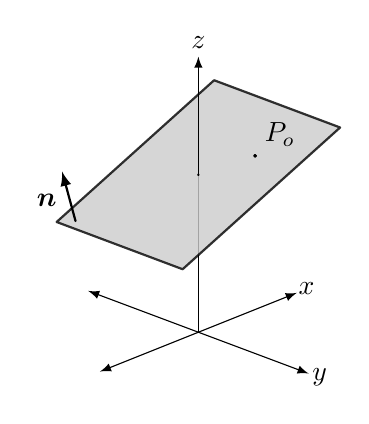
\begin{tikzpicture}[x={(1cm,0.4cm)}, y={(8mm, -3mm)}, z={(0cm,1cm)}, line cap=round, line join=round, scale=0.5]
\def\t{0.9}
\def\s{0.04}
\def\tt{0.3}
\def\ss{0.7}
\def\ttt{0.5}
\def\sss{0.5}
	%Coordinates
	%Plane Vertex Points
	\coordinate (x1) at (-2,2,3);
	\coordinate (x2) at (2,2,5);
	\coordinate (x3) at (2,-2,5);
	\coordinate (x4) at (-2,-2,3);
	%Vectors Parallel to Plane
	\coordinate (n1) at ($(x2) - (x1)$);
	\coordinate (n2) at ($(x2) - (x3)$); 
	%Points on Plane
	\coordinate (x5) at ($(x1) + \s*(n1) - \t*(n2)$);
	\node[outer sep = 1pt, inner sep = 1pt] (x6) at ($(x1) + \ss*(n1) - \tt*(n2)$) {};
	\coordinate (x7) at ($(x1) + \sss*(n1) - \ttt*(n2)$);
	%Beginning of Axis
	\coordinate (O) at (0,0,0);
	%Random Point
	\node[outer sep = 1pt, inner sep = 1pt] (P) at (2.5,1,5.5) {};
	
	%Axis 	
	\draw[latex-latex] (-2.5,0,0) -- (2.5,0,0) node[pos = 1.05] {$x$};
	\draw[latex-latex] (0,-3.5,0) -- (0,3.5,0) node[pos = 1.05] {$y$};
	\draw[-latex] (0,0,0) -- (0,0,7) node[pos = 1.05] {$z$};
	%\draw[draw=black, fill=black] (O) circle (1pt) node[below] {${O}$};
	
	%Point on Plane
	%\draw[-latex, thick] (O) -- (x6) node[pos=0.45, shift={(0.1,0.3)}] {$\vb{r_o}$};
	%Plane
	\path[draw=black, fill=black!20, thick, opacity = 0.8] (x1) -- (x2) -- (x3) -- (x4) -- (x1);
	%\node[shift={(-0.45,0.6)}] at (x3) {$P$};
	%Perpendicular Vector
	\draw[-latex, thick] (x5) -- ($(x5)!0.07!(-8,0,24)$) node[pos=0.5, shift={(-0.2,-0.1)}] {$\bm{n}$};
	%Point on Plane	
	\draw[draw=black, fill=black] (x6) circle (1pt) node[above right] {${P_o}$};
	
	%Z-axis Section
	\draw[draw=black, fill=black] (x7) circle (0.5pt);
	\draw (x7) -- (0,0,6.5);
	
%	%Random Point
%	\draw[-latex, thick] (O) -- (P) node[pos=0.45, shift={(0.1,0.3)}] {$\vb{r}$};
%	\draw[draw=black, fill=black] (P) circle (1pt) node[above right] {$\mathrm{P}$};
	
\end{tikzpicture}
	\end{center}

    
    \end{definition}

    
    \begin{theorem}
    The plane $P$ in $\R^3$ determined by a point $P_0 = (x_0, y_0, z_0)$ and a \textbf{normal vector} $\bm{n} = \langle a, b, c \rangle$ is described by the equations:
    
    \begin{align*}
        \textnormal{Vector form:} \qquad & \bm{n} \cdot \langle x, y , z \rangle &= d \\
        \textnormal{Scalar forms:} \qquad &  a(x-x_0) + b(y-y_0) + c(z-z_0) &= 0 \\
         & ax + by + cz &= d
    \end{align*}
    
    Where we set $d = ax_0 + by_0 + cz_0$.
    
    \end{theorem}


\begin{proposition}
    Given a vector $\bm{n} \in \R^n$, the set $$\{\bm{v} \in \R^n \ | \ \bm{v} \cdot \bm{n} = 0\}$$ is a vector subspace of $\R^n$ of dimension $n-1$.
\end{proposition}


From the previous proposition, we can now generalize our examples from $\R^2$ and $\R^3$:

\begin{definition}
Let $\bm{n} \in V$, with $\bm{n} \neq \bm{0}$.  The \textbf{hyperplane} $W$ normal to $\bm{n}$ (passing through the origin) is the subspace $$W = \{ \bm{v} \in V \ | \ \bm{n} \cdot \bm{v}  = 0 \}$$
We say that $\bm{n}$ is a normal vector of $W$.
\end{definition}


Observe that we can also use vector addition to describe arbitrary planes in $\R^n$ - that is, in order to define a plane $P$ in $\R^n$ (not necessarily passing through the origin), we simply need to describe a point on the plane $P$, and two non-parallel vectors.  That is, we are describing planes as two-dimensional objects in the following way:

\begin{definition}
    The plane $\mathscr{P}$ through the point $P = (x_1, \cdots, x_n)$  and determined by two non-parallel vectors $\bm{u}, \bm{v} \in \R^n$, can be described by the vector function $\bm{r}(s,t) : \R^2 \to \R^n$ defined by 
    $$\bm{r}(s,t) = \bm{r_0} + s\bm{u} + t\bm{v}$$
    where $\bm{r_0}$ is the vector $\bm{r_0} = \bm{OP} = \langle x_1, \cdots, x_n\rangle$.
    
    We call $\bm{r}(s,t)$ the \textbf{parametrization of} $\mathscr{P}$.
    
    \end{definition}
    
    That is, the plane is the set of all linear combinations of $\bm{u}$ and $\bm{v}$ that originate from $P$.

    \begin{remark}
    In other words, we are describing a plane as the image of of a linear map, whereas we can also describe the plane as the kernel of a linear map.
    \end{remark}


\begin{motivating}
How can we reconcile these two notions?
\end{motivating}

This leads us to the notion of the cross product of vectors in $\R^3$.




\subsection{Cross product}

We saw previously that two non-zero vectors in $\R^3$ span a plane $P$ in $\R^3$.  Is there a way to determine the normal vector $\bm{n}$ associated to this plane?

\begin{motivating}

In other words, given two vectors $\bm{u}, \bm{v} \in \R^3$, can we construct a vector $\bm{w} \in \R^3$ that is orthogonal to both $\bm{u}$ and $\bm{v}$?
\end{motivating} 

The answer is yes (at least, in $\R^3)$. We will define the cross product of two vectors in $\R^3$ in a few different ways (see definition \ref{crossproddirmag}, definition \ref{crossproddet}, and theorem \ref{crossprodcomponents}).  Each of these ways has its strengths.

We will first define the cross product in terms of direction and magnitude.

It turns out that in order to describe the direction of the cross product, we will need to make an arbitrary choice. This choice is called the right hand rule: 

\begin{definition}
    We say that an ordered list of three orthogonal vectors $\bm{u}$, $\bm{v}$ and $\bm{w}$ in $\R^3$ satisfy the \textbf{Right Hand Rule}\define{Right Hand Rule} if the following is true.
    
    \begin{enumerate}
        \item Point the fingers of your right hand in the direction of $\bm{u}$
        \item Curl your fingers towards $\bm{v}$ (maybe rotating your hand!)
        \item If your thumb points in the direction of $\bm{w}$, then $\bm{u}$, $\bm{v}$ and $\bm{w}$ satisfy the right hand rule.
    \end{enumerate}
    
    \end{definition}

\textbf{Note that the order matters!} If the ordered list $\bm{u}$, $\bm{v}$ and $\bm{w}$ satisfies the right hand rule, then the ordered list $\bm{v}$, $\bm{u}$ and $\bm{w}$ does not satisfy the right hand rule.

\begin{example}
    For example, consider the standard basis vectors of $\R^3$:  $\bm{i} = \langle 1, 0 , 0 \rangle$, $\bm{j}= \langle 0,1 , 0 \rangle$, and $\bm{k}= \langle 0 , 0,1 \rangle$.

    We see that the ordered list $\bm{i}$, $\bm{j}$, and $\bm{k}$ does satisfy the right hand rule, while the ordered list $\bm{i}$, $\bm{k}$, and $\bm{j}$ doesn't.
\end{example}


We can now define the cross product in terms of direction and magnitude.

\begin{definition}[Magnitude and Direction]\label{crossproddirmag}
    Given two vectors $\bm{u}, \bm{v} \in \R^3$, with an angle $\theta$ between them, their \textbf{cross product}\define{cross product} is the \textnormal{unique} vector $\bm{u \times v} \in \R^3$ with the following properties:
    \begin{enumerate}[label=(\roman*)]
        \item $\bm{u \times v}$ is orthogonal to both $\bm{u}$ and $\bm{v}$.
        \item $\bm{u}$, $\bm{v}$, and $\bm{u \times v}$ satisfies the Right Hand Rule. 
        \item $||\bm{u \times v}|| = ||\bm{u}|| \ ||\bm{v}|| \sin(\theta)$
    \end{enumerate}
    
    Geometrically, we can draw the cross product as follows:
    
    \begin{center}
        \begin{tikzpicture}
\draw (0.6,0) arc [start angle=0,end angle=45,radius=0.6]
node[pos=0.7,right]{$\theta$};
\draw[thick,-Latex,UCLAblue](0,0)--(2,0)node[midway,below]{$\bm{u}$};
\draw[thick,-Latex,megreen](0,0)--(1,1)node[midway,above]{$\bm{v}$};
\draw[thick,-Latex,](0,0)--(0,3)node[pos=0.7,left]{$\bm{u \times v}$};
\end{tikzpicture}
    \end{center}
    
    \end{definition}



Note that together, $(i)$ and $(ii)$ specify a unique direction for the cross product - in $\R^3$, the set of vectors orthogonal to both $\bm{u}$ and $\bm{v}$ spans a one-dimensional subspace (a.k.a. a line).  Thus, to specify one out of the two directions in this line, we must make an arbitrary choice via the right hand rule.  Specifying a magnitude via $(3)$ thus gives us a unique vector.  We will discuss later the choice of magnitude later in \ref{crossprodmagnitudeexp}.

\begin{example}
    What is the cross product $\bm{i} \times \bm{j}$?
\end{example}

\begin{example}
    What is the cross product $\bm{j} \times \bm{k}$?
\end{example}

\begin{motivating}
How can we compute the cross product algebraically?  In other words, what are the components of the cross product?
\end{motivating}

We now give a second, algebraic definition of the cross product.  This will lead to a formula for the components of the cross product (theorem \ref{crossprodcomponents}).


\begin{definition}[Algebraic characterization]\label{crossproddet}
    Given two vectors $\bm{u}, \bm{v} \in \R^3$, their \textbf{cross product}\SubIndex{cross product} is the \textnormal{unique} vector $\bm{u \times v} \in \R^3$ defined by the property:
    \begin{equation*}
(\bm{u \times v}) \cdot \bm{w} = \textnormal{det}
\begin{bmatrix}
\bm{u}\\
    \bm{v}  \\
    \bm{w}
\end{bmatrix} \qquad \textnormal{for all } \bm{w} \in \R^3
\end{equation*}
    
    \end{definition}

This is an interesting perspective on defining a vector in $\R^3$: it is determined by how it relates to all other vectors in $\R^3$.  This kind of idea shows up a lot in higher level mathematics!

First of all, using this algebraic perspective, we can prove the following properties of the cross product: 

\begin{theorem}
    
    Given two vectors $\bm{u}, \bm{v} \in \R^3$,
    
    \begin{enumerate}
        \item $\bm{u} \times \bm{v} = - \bm{v} \times \bm{u}$ (anti-commutativity).
        \item $\bm{u} \times \bm{v}$ is orthogonal to $\bm{u}$ and $\bm{v}$.
        \item The cross product $\times : \R^3 \to \R^3 \to \R^3$ is bilinear.
        \item $\bm{u} \times \bm{v} = \bm{0}$ if and only if $\bm{u}$ and $\bm{v}$ are parallel.
    \end{enumerate}
    
    \end{theorem}

Moreover, we can use the algebraic characterization of the cross product to find the components of the cross product.  Recall from proposition \ref{coeffdotprod}, if we consider the standard basis for $\R^3$, $\mathscr{B} = \{ \bm{e_1}, \bm{e_2},\bm{e_3}\}$, we have that 
\begin{align*}
        \bm{u \times v} &=  (\bm{u \times v}\cdot \bm{e_1}) \bm{e_1} + (\bm{u \times v}\cdot \bm{e_2}) \bm{e_2} + \langle(\bm{u \times v}\cdot \bm{e_3}) \rangle \bm{e_3} \\
        &= \textnormal{det}
\begin{bmatrix}
\bm{u}\\
    \bm{v}  \\
    \bm{e_1}
\end{bmatrix}\bm{e_1} + \textnormal{det}
\begin{bmatrix}
\bm{u}\\
    \bm{v}  \\
    \bm{e_2}
\end{bmatrix}\bm{e_2} + \textnormal{det}
\begin{bmatrix}
\bm{u}\\
    \bm{v}  \\
    \bm{e_3}
\end{bmatrix}\bm{e_3} \\
    &= 
    \left\langle\textnormal{det}
\begin{bmatrix}
\bm{u}\\
    \bm{v}  \\
    \bm{e_1}
\end{bmatrix}, \  \textnormal{det}
\begin{bmatrix}
\bm{u}\\
    \bm{v}  \\
    \bm{e_2}
\end{bmatrix}, \ \textnormal{det}
\begin{bmatrix}
\bm{u}\\
    \bm{v}  \\
    \bm{e_3}
\end{bmatrix} \right\rangle
    \end{align*}

Thus, given the components of two vectors two vectors $\bm{u}, \bm{v} \in \R^3$, we can compute the components of the cross product $\bm{u \times v}$.

\begin{theorem}\label{crossprodcomponents}
    
    Given two vectors $\bm{u} = \langle x_1, y_1, z_1 \rangle$ and $\bm{v}= \langle x_2, y_2, z_2 \rangle$, their \textbf{cross product}\SubIndex{cross product} $\bm{u \times v}$ can described as:
    \begin{align*} \bm{u \times v} &= 
\left\langle \  \textnormal{det}\begin{bmatrix}
y_1 & z_1 \\
y_2 & z_2
\end{bmatrix}, \  - \textnormal{det}\begin{bmatrix}
x_1 & z_1 \\
x_2 & z_2
\end{bmatrix}, \ \textnormal{det}\begin{bmatrix}
x_1 & y_1  \\
x_2 & y_2  \\
\end{bmatrix} \ \right\rangle \\
&= 
\langle y_1z_1 - y_2z_1, \ x_2z_1 - x_1z_2, \ x_1y_2-x_2y_1  \rangle \\
\end{align*}
    
\end{theorem}


We saw previously that two non-zero, non-parallel vectors in $\R^3$ (or equivalently, 3 non-collinear points) span a plane $P$ in $\R^3$, and we can now determine the normal vector $\bm{n}$ associated to this plane:

\begin{example}
    Find the equation for the plane $P$ determined by the points $P = (1,0,-1)$, $Q = (2,2,1)$, $R = (4,1,2)$.
    
    Observe that $\bm{PQ} \times \bm{PR}$ is orthogonal to the plane, and we can use any of $P$, $Q$, or $R$ to determine the plane.
\end{example}



\begin{motivating}
How are these two definitions of the cross product related to each other?
\end{motivating}

In other words, (1) what does the right hand rule have to do with determinants?  (2) why did we choose the magnitude of $\bm{u \times v}$ to be $||\bm{u}|| \ ||\bm{v}|| \sin(\theta)$?

More generally, what is the geometry of the determinant?

    \begin{proposition}
        The right hand rule corresponds to having a positive determinant.
    \end{proposition}

\fixthis{explain} (relaxed right-hand rule, adding scalar multiples does not change right-handedness - turn into diagonal matrix).

\begin{example}
    The standard basis $\{\bm{i}, \bm{j}, \bm{k}\}$ satisfies the right hand rule, and $\det\begin{bmatrix}
\bm{e_1}\\
    \bm{e_2}  \\
    \bm{e_3}
\end{bmatrix}$ has positive determinant.
\end{example}


We now turn to question 2: Why did we choose the  magnitude of $\bm{u \times v}$ to be $||\bm{u}|| \ ||\bm{v}|| \sin(\theta)$?

\begin{proposition}\label{crossprodmagnitudeexp}
        Given two vectors $\bm{u}, \bm{v} \in \R^3$, with an angle $\theta$ between them, then $$||\bm{u \times v}|| = ||\bm{u}|| \ ||\bm{v}|| \sin(\theta)$$
    \end{proposition}
    
First, observe that if two non-parallel vectors (say, $\bm{u}, \bm{v} \in \R^3$) start at the same point, then they uniquely determine a triangle, and a  parallelogram.
\begin{center}
            \begin{tikzpicture}scale=0.5]
                \begin{scope}
            \pgfmathsetmacro{\cubex}{2}
            \pgfmathsetmacro{\cubey}{3}


    \draw[fill=rosequartz!30,opacity=0.6] (0,0) -- (\cubex,1) -- (0,\cubey-1) -- cycle;

    \draw[red, thick, -Latex] (0,0) -- (\cubex,1) node[midway,below right] {$\bm{u}$};
    \draw[megreen, thick, -Latex] (0,0) -- (0,\cubey-1) node[midway, left] {$\bm{v}$};
    
    
    \end{scope}
            
            \begin{scope}[xshift=4cm]
            
            \pgfmathsetmacro{\cubex}{2}
            \pgfmathsetmacro{\cubey}{3}
    
    \draw[fill=rosequartz!30,opacity=0.6] (0,0) -- (\cubex,1)  -- (\cubex,\cubey) -- (0,\cubey-1)-- cycle;
    
    \draw[red, thick, -Latex] (0,0) -- (\cubex,1) node[midway,below right] {$\bm{u}$};
    \draw[megreen, thick, -Latex] (0,0) -- (0,\cubey-1) node[midway,left] {$\bm{v}$};
    
            \end{scope}
    
    

    
    \end{tikzpicture}
        \end{center}

\begin{theorem}
    Let $P$ be the parallelogram spanned by $\bm{u}$ and $\bm{v}$, and $T$ be the triangle spanned by $\bm{u}$ and $\bm{v}$. Then
    $$\textnormal{area}(P) =  ||\bm{u \times v}|| \qquad \textnormal{and} \qquad \textnormal{area}(T) = \frac{1}{2}||\bm{u \times v}||$$
\end{theorem}

Observe that by geometry, the area of $P$ is twice the area of the triangle $T$.  Furthermore, if the angle between $\bm{u}$ and $\bm{v}$ is $\theta$, we can calculate the area of the parallelogram as begin base times height, e,g, $$(||\bm{u}||)(||\bm{v}||\sin(\theta)) = ||\bm{u \times v}||$$

However, here's another way to think about this parallelogram: Without loss of generality, we can rotate our vectors so that they lie in the $xy$-plane.  (Equivalently, we can choose a basis $\mathcal{B}$ so that the coordinates of $\bm{u} = \langle a, b, 0 \rangle$, and that $\bm{v} = \langle c, d, 0 \rangle$).

\begin{figure}[H]
    \centering
    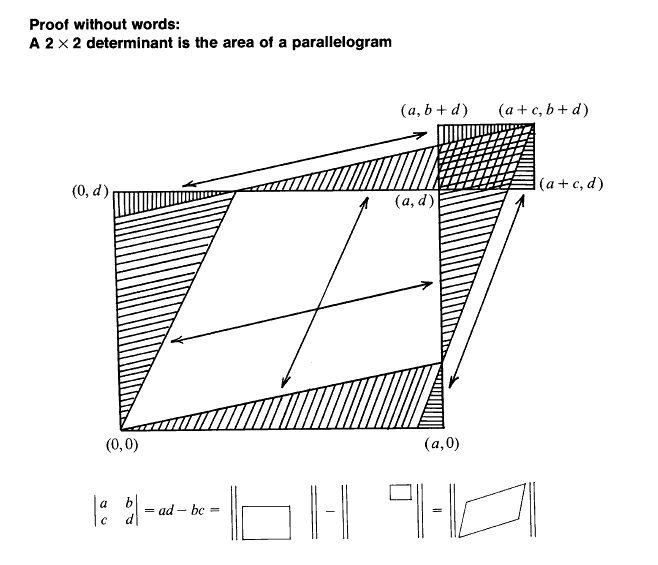
\includegraphics[scale=0.5]{images/2x2detproof.png}
    \caption{A Proof without Words, by Solomon W. Golomb (\href{https://www.tandfonline.com/doi/abs/10.1080/0025570X.1985.11977163}{Mathematics Magazine, March 1985})}
\end{figure}

Observe that the figure above shows that \begin{equation*}
        \Big|\textnormal{det}\begin{bmatrix}
a & b \\
c & d
\end{bmatrix}\Big| = \textnormal{area}(P)
    \end{equation*}
    
       That is, the absolute value of a $2 \times 2$
determinant equals the area of the parallelograms spanned by the rows.  

In other words, the determinant of a $2 \times 2$ matrix $A$ measures the area of the parallelogram spanned by $A\bm{e_1} = \langle a, c \rangle $ and $A\bm{e_2} = \langle b, d \rangle$.   That is, it measures the area of the image of the unit square under the linear transformation $T: \R^2 \to \R^2$ defined by $T(\bm{v}) = A\bm{v}$.

\begin{motivating}
Does this generalize to linear transformations in higher dimensions?
\end{motivating}

\begin{definition}
    
Given three vectors $\bm{u}$, $\bm{v}$, and $\bm{w}$ in $\R^3$, they span a \textbf{parallelpiped}\define{parallelpiped}.  That is, a 3-dimensional solid, such that each face is a parallelogram.

\begin{center}
    
    \begin{tikzpicture}[scale=.7]
    \newcommand{\Depth}{3}
    \newcommand{\Height}{2.5}
    \newcommand{\Width}{4}
    \newcommand{\Skew}{1}

    \coordinate (a) at (0,0,0);
    \coordinate (b) at (\Width,0,0);
    \coordinate (c) at (\Width + \Skew,\Height,\Skew);
    \coordinate (d) at (\Skew,\Height,\Skew);
    \coordinate (e) at (0,0,\Depth);
    \coordinate (f) at (\Width,0,\Depth);
    \coordinate (g) at (\Width + \Skew,\Height,\Depth + \Skew);
    \coordinate (h) at (\Skew,\Height,\Depth + \Skew);

    \coordinate (i) at (\Skew,5,\Depth+ 2.5);

    \draw[fill=rosequartz!30,opacity=0.6] (a) -- (b) -- (c) -- (d) -- (a);
    \draw[fill=rosequartz!30,opacity=0.6] (a) -- (e) -- (f) -- (b) -- (a);
    \draw[fill=rosequartz!30,opacity=0.6] (a) -- (d) -- (h) -- (e) -- (a);
    \draw[fill=rosequartz!30,opacity=0.6] (d) -- (c) -- (g) -- (h) -- (d);
    \draw[fill=rosequartz!30,opacity=0.6] (e) -- (f) -- (g) -- (h) -- (e);
    \draw[fill=rosequartz!30,opacity=0.6] (b) -- (c) -- (g) -- (f) -- (b);
    
    \draw[red, thick, -Latex] (e) -- (h) node[midway,right] {$\bm{u}$};
    \draw[megreen, thick, -Latex] (e) -- (a) node[midway,right] {$\bm{v}$};
    \draw[UCLAblue, thick, -Latex] (e) -- (f) node[midway, below left] {$\bm{w}$};
    
    \draw[dashed, -Latex] (e) -- (i) node[midway, left] {$\bm{v \times w}$};
    
    % \node[place, label=below right:{(4,2,1)}] at (a) {};
    % \node[place, label=right:{(1,7,1)}] at (b) {};
    % \node[place, label=above:{(2,9,7)}] at (c) {};
    % \node[place, label=above:{(5,4,7)}] at (d) {};
    % \node[place, label=below:{(8,1,0)}] at (e) {};
    % \node[place, label=below:{(5,6,0)}] at (f) {};
    % \node[place, label=above left:{(6,8,6)}] at (g) {};
    % \node[place, label=left:{(9,3,6)}]  at (h) {};

\end{tikzpicture}
    
\end{center}
\end{definition}

We can again use geometry to compute the volume of this parallelpiped:

\begin{theorem}
    Let $D$ be the parallelpiped spanned by $\bm{u}$, $\bm{v}$, and $\bm{w}$, and let $\theta$ be the angle between $\bm{u}$ and $\bm{v \times w}$. Then $$\textnormal{volume}(D) = ||\bm{v \times w}|| \ ||\bm{u}|| \ |\cos(\theta)|$$
    \end{theorem}

Observe that we can write this formula in terms of a dot product.

\begin{definition}
        The scalar $\bm{u} \cdot (\bm{v \times w})$ is called the \textbf{scalar triple product}\define{scalar triple product}.
\end{definition}

\begin{example}
Let $D$ be the parallelpiped spanned by $\bm{u} = \langle 1, 3, 2 \rangle$, $\bm{v} = \langle 6, 5, 4 \rangle$, and $\bm{w} = \langle 2, 2, 2 \rangle$.  Compute the volume of $D$.

\end{example}

This computation should seem familiar to you: see example \ref{det3d}

\begin{theorem}
    Let $D$ be the parallelpiped spanned by $\bm{u} = \langle u_1, u_2, u_3 \rangle$, $\bm{v} = \langle v_1, v_2, v_3 \rangle$, and $\bm{w} = \langle w_1, w_2, w_3 \rangle$.  Then
    \begin{equation*}
\textnormal{volume}(D) = |\bm{u} \cdot (\bm{v \times w})| = | \textnormal{det}
\begin{bmatrix}
\bm{u} \\
\bm{v} \\
\bm{w} \\
\end{bmatrix}|
\end{equation*}

    \end{theorem}


\begin{example}
    \begin{definition}
        We say that three vectors $\bm{u}, \bm{v}, \bm{w} \in \R^n$ are \textbf{co-planar}\define{co-planar} if they all lie in the same plane. 
    \end{definition}
    
    Show that if $\bm{u}, \bm{v}, \bm{w} \in \R^3$ are co-planar, then $\textnormal{volume}(D) = 0$.  What is the geometric interpretation of this fact?
\end{example}

Just as we saw in the $2 \times 2$ case, we see again that the determinant of a $3 \times 3$ matrix $A$ measures the volume of the parallelpiped spanned by $A\bm{e_1}$, $A\bm{e_2}$, and $A\bm{e_3}$.  That is, it measures the volume of the image of the unit cube under the linear transformation $T: \R^2 \to \R^2$ defined by $T(\bm{v}) = A\bm{v}$.

This generalizes to $n \times n$ matrices and their associated linear transformations $T:\R^n\to \R^n$.  The determinant will measure the $n$-dimensional volume of the $n$-dimensional parallelpiped spanned by the image of the unit $n$-cube.  In other words, the absolute value of $\textnormal{det}A$ is the factor by which $T$ magnifies volume; and $\textnormal{det}A$ is zero if and only if T is not invertible. 



    \begin{quote}
        ``The determinant is astonishing."       --- Jerry Shurman, \textnormal{Calculus and Analysis in Euclidean Space}.
    \end{quote}








\subsection{Inner products}

\begin{motivating}
How can we generalize the dot product in  $\R^n$ to an arbitrary vector space $V$?  
\end{motivating}

For $\R^n$, we saw that the dot product satisfies the property $\bm{v} \cdot \bm{v} = ||\bm{v}||^2$. Thus, our generalization should allow us to define a notion of \underline{distance} in an abstract vector space.

\begin{definition}
    
    Given two vectors $\bm{u},\bm{v} \in V$, an \textbf{inner product}\define{inner product} on $V$ is a map $\langle - , - \rangle :  V \times V \to \R$ that is:
    \vspace{1em}
    
    \begin{enumerate}
        \item $\langle \bm{u}, \bm{v} \rangle = \langle \bm{v}, \bm{u} \rangle$ (symmetric).
        \item $\langle - , - \rangle$ is bilinear.
        \item $\langle \bm{v}, \bm{v} \rangle \geq 0$, with equality only when $\bm{v} = \bm{0}$. (positive definite).  
    \end{enumerate}
    
    \end{definition}

\begin{definition}
    Given an innner product$\langle - , - \rangle$ on $V$, the \textbf{norm} (or \textbf{modulus}) of a vector $\bm{v} \in V$ is defined as $$||\bm{v}|| = \sqrt{\langle \bm{v}, \bm{v}\rangle}$$
    \end{definition}
    

\begin{example}
    Given two vectors $\bm{u} = \langle u_1, \cdots, u_n \rangle$ and $\bm{v}  = \langle v_1 , \cdots, v_n \rangle$ in $\R^n$, their \textbf{dot product} is an inner product. $$\bm{u} \cdot \bm{v} = \sum u_iv_i$$
    \end{example}

\begin{theorem}[Properties of an inner product]
    
    \begin{enumerate}
        \item Cauchy-Schwarz inequality: $| \langle \bm{u},\bm{v} \rangle | \leq  | \bm{u}| \ | \bm{v} |$
        \item Triangle inequality: $| \bm{u}+ \bm{v} | \leq  | \bm{u}| +| \bm{v} |$
    \end{enumerate}
    
    \end{theorem}





\begin{motivating}
What is the geometric interpretation of the inner product for an arbitrary vector space?
\end{motivating}

\begin{definition}
    A subset $S = \{\bm{v_1}, \bm{v_2}, \cdots, \bm{v_k}\} \subseteq V$ is said to be \textbf{orthogonal} if $\langle \bm{v_i}, \bm{v_j} \rangle = 0$ for all $i \neq j$.
    
    \vspace{1em}
    
    Furthermore, if $|\bm{v_i}| = 1$ for all $1 \leq i \leq k$, we say that the subset $S = \{\bm{v_1}, \bm{v_2}, \cdots, \bm{v_k}\} \subseteq V$ is \textbf{orthonormal}.
\end{definition}
    
    \begin{proposition}
        Equivalently, a set subset $S = \{\bm{v_1}, \bm{v_2}, \cdots, \bm{v_k}\} \subseteq V$ is orthonormal if $$\langle \bm{v_i}, \bm{v_j} \rangle = \delta_{ij}$$ 
        where $\delta_{ij}$ is the \textbf{Kronecker delta}, which is the symbol $$\delta_{ij} = \left\{
		\begin{array}{ll}
			1 & \text{ if } i = j \\
			0 & \text{ if } i \neq j
		\end{array}
		\right.$$
    \end{proposition}


\subsection{Exercises}

\begin{problem}{orthogonal1}
     Find all values of $b$ such that the vectors $\bm{u} = \langle b,3,2\rangle$ and $\bm{v} = \langle 1,b,1\rangle$ are orthogonal.
\end{problem}

\begin{problem}{axiomcalc}
    Given that $||\bm{u}|| = 1$, $||\bm{v}|| = 3$, and $\bm{u} \cdot \bm{v} = 2$, evaluate the expression $2\bm{u} \cdot (3\bm{u} - \bm{v})$.
\end{problem}

\begin{problem}{axiomcalc2}
    Given that $||\bm{u}|| = 2$, $||\bm{v}|| = 3$, and the angle between $\bm{u}$ and $\bm{v}$ is $120^\circ$, calculate $||3\bm{u}-\bm{v}||^2$.
\end{problem}

\begin{problem}{triangle}
    Consider the points $P= (0,8,3)$, $Q= (1,3,0)$, and $R= (1,5,-2)$.   Does the triangle $PQR$ have (A) an obtuse angle (and two acute angles); (B) a right angle (and two acute angles); or (C) three acute angles?
\end{problem}

\begin{problem}{projection}
    Consider the points $P= (0,8,3)$, $Q= (1,3,0)$, and $R= (1,5,-2)$, find the projection of $\bm{PQ}$ in the direction of $\bm{PR}$.
\end{problem}

\begin{problem}{projection2}
    Find the projection of $\bm{u} = \langle 5,7,-4\rangle$ along $\bm{v} = \langle0,0,1\rangle$.
\end{problem}

\begin{problem}{projection3}
    Find the projection of $\bm{u} = \langle a,a,b\rangle$ along $\bm{v} = \bm{i} - \bm{j}$.
\end{problem}

\begin{problem}{projection4}
    Given $\bm{u} = \langle 4, -1, 2 \rangle$, and $\bm{v} = \langle 1, 0, 1 \rangle$
    
    \begin{subproblems}
    \item Find the vectors $\bm{u}_{||\bm{v}}$ and $\bm{u}_{\bot\bm{v}}$
    \item Find the vectors $\bm{v}_{||\bm{u}}$ and $\bm{v}_{\bot\bm{u}}$
    \end{subproblems}
    
\end{problem}


\begin{problem}{plane}
    Write the equation of the plane in $\R^3$ with normal vector $\bm{n} = \langle-1,2,1\rangle$ passing through the point $(4,1,5)$.
\end{problem}

\begin{problem}{plane2}
    Find the equation of the plane in $\R^3$  passing through the points $P = (5,1,1)$, $Q = (1,1,2)$, $R = (2,1,1)$.
\end{problem}

\begin{problem}{plane3}
    Find the equation of the plane in $\R^3$ that contains the lines $$\bm{r_1}(t)= \langle 2 + t, 2 + 3t, 3+ t \rangle$$ $$\bm{r_2}(s)= \langle 5 + s, 15 + 4s, 10 + 2s \rangle$$
\end{problem}

\begin{problem}{plane4}
    Consider the plane $P$ in $\R^3$ given by the equation $3x + 5y-2z = 29$. Find the equation of the plane $R$ that is parallel to $P$ and passes through the point $(3,-1,1)$.
\end{problem}


\begin{definition}
    Let $A$ be a nonempty subset of an inner product space $V$.  The \textbf{orthogonal complement} of $A$ is the subspace
    $$A^\bot := \{\bm{v} \in V \ | \ \langle \bm{a}, \bm{v} \rangle = 0 \ \text{for every } \bm{a} \in A \}$$
    \end{definition}

\begin{problem}{Subspacenk}
    
    
    Prove that $A^\bot$ is a vector subspace.  
    
    
    Let $A = \{\bm{u_1}, \cdots \bm{u_k}\}$ be $k$ linearly independent vectors in a vector space $V$ of dimension $n$. Prove that $A^\bot$ is a subspace of dimension $n-k$.
    
    Describe $A^\bot$ is the intersection of $k$ hyperplanes.
    
\end{problem}

\begin{problem}{crossprodcalc}
    Calculate the cross product of $\bm{u} = \langle 1,1,0\rangle$ and $\bm{v} = \langle 0,1,1\rangle$
\end{problem}

\begin{problem}{parallelogram}
    Consider the points $P= (0,8,3)$, $Q= (1,3,0)$, and $R= (1,5,-2)$, find the area of the parallelogram spanned by   $\bm{PQ}$ and  $\bm{PR}$.
\end{problem}

\begin{problem}{parallelogram2}
    Find the area of the parallelogram determined by the vectors $\langle a, 0, 0\rangle$ and $\langle 0, b, c\rangle$
\end{problem}

\begin{problem}{trianglecross}
    Consider the points $P= (0,8,3)$, $Q= (1,3,0)$, and $R= (1,5,-2)$, find the area of the triangle spanned by   $\bm{PQ}$ and  $\bm{PR}$.
\end{problem}

\begin{problem}{parallelpiped1}
    Consider the points $P= (-1,8,3)$, $Q= (2,3,0)$, $R= (2,5,-2)$, and $S = (3,5,2)$. Find the volume of the parallelpiped that has vertices $P$, $Q$, $R$, and $S$.
    
\end{problem}

\begin{problem}{parallelpiped2}
    Find the volume of the parallelpiped in $\R^3$ spanned by the vectors $\bm{u} =\langle 1, 0,4 \rangle$, $\bm{v} = \langle 1, 3, 1 \rangle$, $\bm{w} = \langle -4, 2, 6 \rangle$.
\end{problem}

\begin{problem}{parallelpiped3}
    Let $P$ be the parallelpiped contained in the first octant (that is, all points in $P$ satisfy $x \geq 0$, $y \geq 0$, $z \geq 0$) determined by the vertices $A= (2,4,1)$, $B= (5,2,5)$, $C= (1,2,4)$, and $D = (1,1,1)$. Find the point $X$ in the parallelpiped $P$ that is \textbf{furthest} from the origin. (\textbf{Hint:} Draw a picture).
\end{problem}

\begin{problem}{lineorplane}
    Do the points $P = (0,1,1)$, $Q = (1,1,2)$, $R = (3,3,3)$ determine a plane or a line?  Find the equation of either the plane or the line.
\end{problem}

\begin{problem}{planesandlines}
    Let $P$ be the plane given by the equation $-3x - 4y+2z = -10$. The plane $P$ intersects the plane $z=0$ at some \textbf{acute} angle $\theta$.  Determine the value of $\cos(\theta)$.
\end{problem}

\begin{problem}{lineplane}
    The intersection of the plane $-3x - 4y+2z = -10$ and the plane $z=0$ is a line $L$.  Find a vector parametrization of the line $L$.
\end{problem}

\begin{problem}{lineintersect}
    The line $\bm{r}(t) = \langle 2, 2, 8 \rangle + t\langle 0,1,2\rangle$ intersects the sphere $x^2 + (y+3)^2 + (z+2)^2 = 9$ in two points.  Find these two points.
\end{problem}

\chapter{Analysis on $\R^n$}
Having studied the vector space structure on $\R^n$, we will now turn to the geometric and topological properties of $\R^n$

\section{Multivariable functions}

\subsection{Vector-valued functions}

$f : \R \mapsto \R^n$

\subsection{Multivariable functions}

$f : \R^m\mapsto \R$

\subsection{General Multivariable functions}

$f : \R^m\mapsto \R^n$

\subsection{Exercises}

We say that two lines $\bm{r_1}(t)$ and $\bm{r_2}(s)$ \textbf{intersect} if there is a point $P$ lying on both curves.  We say that $\bm{r_1}(t)$ and $\bm{r_2}(s)$ \textbf{collide} if there exists some $t_0$ such that $\bm{r_1}(t_0) = \bm{r_2}(t_0)$.


\section{Limits}

\subsection{Limits of sequences}

\subsection{Limits of vector valued functions}

\subsection{Limits of multivariable functions}

\subsection{General Multivariable functions}

$f : \R^m\mapsto \R^n$

\section{Continuity}

\subsection{Vector-valued functions}

\subsection{Multivariable functions}

$f : \R^m\mapsto \R$

\subsection{General Multivariable functions}

$f : \R^m\mapsto \R^n$

\chapter{The Multivariable Derivative}


Now that we have understood the notions of limits and continuity, we can turn to defining the notion of the multivariable derivative.

Let us first recall the notion of the derivative of a single-variable function:


\begin{definition}
    A function $f : D \subset \R \to \R$ is \textbf{differentiable} at a point $x_0 \in D$ if 

    \begin{itemize}
        \item There exists $\delta$ such that $B_\delta(x_0) \subseteq D$
        \item The following limit exists:  $$\lim_{h \to 0} \frac{f(x_0+h) - f(x_0)}{h} = L$$
    \end{itemize}

    If $f$ is differentiable at $x_0$, we say that $L$ is \textbf{the derivative of $f$ at $x_0$}, and we write $$f'(x_0) := L$$
    (sometimes written $\frac{df}{dx}(x_0) = L$)
    \end{definition}

In other words, the derivative depends precisely on the local behavior of $f(x)$ near $x_0$.  That is, we look precisely at the behavior of $f(x)$ in a small neighborhood $B_\varepsilon(x_0)$.

\fixthis{interior point}


The notion of the derivative in single-variable calculus has many interpretations:

\begin{itemize}
    \item The derivative $f'(a)$ tells us the slope of the tangent line to the graph $y=f(x)$ at the point $x=a$.
    \item The derivative $f'(a)$ tells us the instantaneous rate of change of $f(x)$ at the point $x=a$.
    \item The derivative $\frac{d}{dx}$ is an operator, whose input is a differentiable function $f : \R \to \R$, and whose output is a function $f' : \R \to \R$.
    \item The derivative is the linear approximation of $f(x)$ in a small neighborhood $B_\varepsilon(x_0)$.
\end{itemize}

We will see how all of these various notions generalize to the case of multivariable functions.


\section{The Multivariable Derivative}

It takes some thought to come up with the correct definition of the derivative of a multivariable function $f : \R^n \to \R$ at a point $\bm{x_0}$!  

For instance, one might na\"ively define the multivariable derivative as the following limit:
$$f'(\bm{x_0}) \ ``=" \ \lim_{\bm{h} \to \bm{0}} \frac{f(\bm{x_0+h})-f(\bm{x_0})}{||\bm{h}||}$$

However, this definition \textbf{fails} for multiple reasons:

\begin{example}\label{derivfail1}
    Let $f : \R^2 \to \R$ be the function $f(x,y) = x$, and consider the point $\bm{x_0} = (0,0)$.  
    
    We see that $$\lim_{(x,y) \to (0,0) } \frac{f(x,y)-f(0,0)}{||\langle x,y\rangle||}$$
    \textbf{does not exist} by considering the following sequences:

    \begin{itemize}
        \item Along the sequence $\bm{x_n} = \langle \frac{1}{n}, 0 \rangle$, we have that $$\lim_{n\to\infty} \frac{f(\frac{1}{n}, 0)}{||\langle \frac{1}{n}, 0\rangle||} = 1$$
        \item Along the sequence $\bm{y_n} = \langle \frac{1}{n}, 0 \rangle$, we have that $$\lim_{n\to\infty} \frac{f(\frac{-1}{n}, 0)}{||\langle \frac{-1}{n}, 0\rangle||} = -1$$
        \item Along the sequence $\bm{z_n} = \langle 0, \frac{1}{n}\rangle$, we have that $$\lim_{n\to\infty} \frac{f(0, \frac{1}{n})}{||\langle 0, \frac{1}{n}\rangle||} = 0$$
    \end{itemize}
    
\end{example}

Moreover, this definition also fails because it does not correctly generalize the notion of the single variable derivative:

\begin{example}\label{derivfail2}
    Specializing the na\"ive definition to $n=1$, we obtain $\lim_{x \to 0 } \frac{f(x)-f(0)}{|x|}$.

    However, if we consider the function $f: \R \to \R$ defined by $f(x) = |x|$.  We know from single-variable calculus that this function is not differentiable at $x=0$.

    Nevertheless, we see that $$\lim_{x \to 0 } \frac{f(x)-f(0)}{|x|} = 1$$
    
\end{example}

\begin{remark}
    One can correct for the issue in \ref{derivfail2} by instead considering $$\lim_{\bm{h} \to \bm{0}} \frac{|f(\bm{x_0+h})-f(\bm{x_0})|}{||\bm{h}||}$$

    Nevertheless, the issue in \ref{derivfail1} continues to exist for the $f(x,y) = x$ at $(0,0)$ by considering the sequences $\bm{x_n} = \langle \frac{1}{n}, 0 \rangle$ and $\bm{z_n} = \langle 0, \frac{1}{n}\rangle$.
\end{remark}

Thus, we must make a paradigm shift in how we think of the multivariable derivative:


\begin{motivating}
    How should we interpret the multivariable derivative?
\end{motivating}


    The derivative of a single variable function $f(x)$ at a point $x_0$ is the \textbf{approximation} of $f(x)$ by a linear transformation at $x_0$.

\begin{definition}
    A single variable function is \textbf{differentiable at }$x_0$ if there exists a linear transformation $T: \R \to \R$ such that 
    
    $$\lim_{h \to 0} \bigg|\frac{f(x_0+h)-f(x_0)-T(h)}{h}\bigg| = 0$$
    
    Observe that by our characterization of linear transformations $T: \R \to \R$, correspond to scalars $m in \R$ via the correspondence    
    $$T(x) = mx$$  
    We define the derivative of $f$ at $x_0$ to be $m$. That is,    
    $$f'(x_0) := m$$
    \end{definition}

We can generalize this definition as follows:

\begin{definition}
    A multivariable function $f : A \subset R^m \to \R^n$ is \textbf{differentiable at}\define{Multivariable derivative} an interior point $\bm{x_0}$ of $A$  if there exists a linear transformation $T: \R^m \to \R^n$ such that 
    
    $$\lim_{\bm{h} \to \bm{0}} \frac{||f(\bm{x_0+h})-f(\bm{x_0})-T(\bm{h})||}{||\bm{h}||} = 0$$
    
    The \textbf{derivative} of $f$ at $x_0$ is the linear transformation $$Df(\bm{x_0}) := T$$

    By our characterization of linear transformations, $Df(\bm{x_0}) : \R^m \to \R^n$ corresponds to a matrix $[Df(\bm{x_0})] \in M_{n\times m}(\R)$
    \end{definition}

\begin{remark}
    The derivative of a function $f : \R^m \to \R^n$ at a point $x_0$ is the \textbf{approximation} of $f$ by a \textbf{linear transformation} $Df(\bm{x_0})$ at $x_0$.
    \end{remark}

    \begin{proposition}[Uniqueness]
    Suppose $f : A \subset \R^m \to \R^n$ is differentiable at $\bm{x_0}$.
       
    \vspace{1em}
    Then the derivative $Df(\bm{x_0}) : \R^m \to \R^n$ is unique.
    \end{proposition}

    \begin{example}        
The constant map $c: \R^m \to \R^n$ defined by $c(\bm{x}) = \bm{a}$ is differentiable everywhere, and $Dc(\bm{x_0}) = 0$.
    \end{example}

    \begin{example}\label{derivlinearmap}
    A linear map $T: \R^m \to \R^n$ is differentiable everywhere, and $DT(\bm{x_0}) = T$.
    \end{example}

    \begin{proposition}
Suppose that $f, g : A \to \R^n$ are differentiable at $x_0  \in A^\circ$. Then $f+g$ and $\lambda f$ are differentiable at $x_0 \in A^\circ$.
\end{proposition}

    \begin{proposition}[Differentiability implies continuity]
    Suppose $f : A \subset \R^m \to \R^n$ is differentiable at $\bm{x_0}$. 
    
    \vspace{1em}
    Then $f$ is continuous at $\bm{x_0}$.
    \end{proposition}

    \begin{theorem}[The Chain rule]
    Suppose that $g: \R^k \to \R^m$ is differentiable at $x_0 \in \R^k$, and $f : \R^m \to \R^n$ is differentiable at $g(\bm{x_0}) \in \R^m$.  
    
    \vspace{1em}
    
    Then $f \circ g : \R^k \to \R^n$ is differentiable at $x_0 \in \R^k$, and 
    $$D(f \circ g)(\bm{x_0}) = D(f)(g(\bm{x_0})) \circ Dg(\bm{x_0})$$
    
    \end{theorem}


\subsection{The derivative of a vector valued function}

\begin{theorem}
    Let $\bm{r}(t) = \langle x_1(t), \cdots, x_n(t) \rangle$ be a vector-valued function.  
    
    The \textbf{derivative} of $\bm{r}(t) : \R \to \R^n$ at an interior point $\bm{t_0}$ is the linear transformation $T: \R \to \R^n$ given by 
    $$T = 
\begin{bmatrix}
x_1'(t_0) \\
\vdots \\
x_n'(t_0) \\
\end{bmatrix}$$
We sometimes write this derivative as $\bm{r}'(t) : \R \to \R^n$.
\end{theorem}


\begin{theorem}
    A vector-valued function $\bm{r}(t)= \langle x_1(t), \cdots, x_n(t) \rangle$ is differentiable if and only if the functions $x_i(t)$ are differentiable.
     $$\bm{r}'(t) = \langle x_1'(t), \cdots, x_n'(t) \rangle$$
\end{theorem}

    We can think of the derivative $\bm{r}'(t)$ as a tangent vector to the parametric curve of $\bm{r}(t)$.


\begin{definition}
    The \textbf{tangent line} at $\bm{r}(t_0)$ is the line determined by the direction vector $\bm{r}'(t_0)$ and the point $\bm{r}(t_0)$.  That is, the line can be parametrized as 
    $$\bm{L}(t) = \bm{r}(t_0) + t\bm{r}'(t_0)$$
    \end{definition}

\fixthis{picture}

\begin{theorem}[Differentiation Rules]
       Assume that $\bm{r}(t)$ and $\bm{s}(t)$ are differentiable vector-valued functions $\R \to \R^n$..
       
      \begin{enumerate}
        \item $\frac{d}{dt}(\bm{r}(t) + \bm{s}(t)) = \bm{r}'(t) + \bm{s}'(t)$ 
        \item \textbf{Scalar product rule}. For any differentiable scalar-valued function $f(t)$, 
        $$\frac{d}{dt}(f(t)\bm{r}(t)) = f(t)\bm{r}'(t) + f'(t)\bm{r}(t)$$   
        \vspace{-1em}
        \item \textbf{Chain rule}. For any differentiable scalar-valued function $f(t)$, $$\frac{d}{dt}(\bm{r}(f(t))) =  \bm{r}'(f(t))f'(t)$$  
    \end{enumerate}
    \end{theorem}

\begin{theorem}[Dot product rule]
       Assume that $\bm{r}(t)$ and $\bm{s}(t)$ are differentiable vector-valued functions $\R \to \R^n$. Then
       $$\frac{d}{dt}(\bm{r}(t) \cdot \bm{s}(t)) = \bm{r}'(t)\cdot\bm{s}(t) + \bm{r}(t)\cdot\bm{s}'(t)$$ 
    \end{theorem}
    
       
    \begin{theorem}[Cross product rule]
       Assume that $\bm{r}(t)$ and $\bm{s}(t)$ are differentiable vector-valued functions $\R \to \R^3$. Then 
       $$\frac{d}{dt}(\bm{r}(t) \times \bm{s}(t)) = \bm{r}'(t)\times \bm{s}(t) + \bm{r}(t)\times \bm{s}'(t)$$
    \end{theorem}

\subsection{The derivative of multivariable functions}

\begin{motivating}
    How should we think of the derivative of a multivariable function $f: \R^n \to \R$?
    \end{motivating}

Given a function $g: \R^n \to \R$, we can graph it as a surface $x_{n+1} = g(x_1, \cdots, x_n)$ in $\R^{n+1}$, which has points $$(x_1,\cdots, x_n, g(x_1, \cdots, x_n))$$
    
    
    If $T$ is the derivative of a function $f: \R^n \to \R$, then $T : \R^n \to \R$ is a linear map, which corresponds to a $n \times 1$ matrix.
    \begin{equation*}
T(x_1, \cdots, x_n) = A\begin{bmatrix}
x_1 \\
\vdots\\
x_n
\end{bmatrix}
=
\begin{bmatrix}
a_1 & \cdots & a_n
\end{bmatrix}\begin{bmatrix}
x_1 \\
\vdots\\
x_n
\end{bmatrix}
= \sum_i^n a_ix_i
\end{equation*}

\begin{proposition}
The graph of $T : \R^n \to \R$ is the hyperplane $x_{n+1} = \sum_i^n a_ix_i$.
\end{proposition}

\begin{definition}
    The \textbf{$i$-th partial derivative} $D_if$ of a multivariable function $f : A \subset \R^m \to \R$ for $\bm{x_0} \in A^\circ$ is defined as the limit
    $$D_if(\bm{x_0}) =  \lim_{t \to 0} \frac{f(\bm{x_0}+t\bm{e_i})-f(\bm{x_0})}{t}, \qquad i = 1, \cdots, n$$
    if it exists.
    
    \end{definition}

    \begin{example}
        Let $f: \R^2 \to \R$ be defined by $f(x,y) = xe^{xy}$.  Then the partial derivatives of $f$ are
        $$\frac{\partial f}{\partial x} = xye^{xy} + e^{xy} \qquad \frac{\partial f}{\partial y} = x^2e^{xy}$$
    \end{example}
    

\begin{proposition}
    Given a graph of $z = f(x_1, \cdots, x_n)$, the tangent (hyperplane) in $\R^{n+1}$ is spanned by vectors of the form $\bm{e_i} + \frac{\partial f}{\partial x_i}\bm{e_{n+1}}$
    \end{proposition}
    
    \fixthis{picture}
    
    \begin{proposition}
    We can take the normal vector of the tangent hyperplane in $\R^{n+1}$ to the graph of a multivariable function $f : \R^n \to \R$ to be 
    $$\bm{n} = \sum_{i}^n \left(\frac{\partial f}{\partial x_i}\bm{e_i}\right) -\bm{e_{n+1}} = \left\langle \frac{\partial f}{\partial x_1}, \cdots, \frac{\partial f}{\partial x_n}, -1\right\rangle $$
    \end{proposition}

    \begin{theorem}
    Let $\bm{a} = \langle a_1, \cdots, a_n \rangle \in \R^n$.  The equation of the tangent hyperplane in $\R^{n+1}$ to the graph of a multivariable function $f(\bm{a}) : \R^n \to \R$ at a point $$\bm{\overline{a}} = (a_1, \cdots, a_n, f(\bm{a}))$$ is given by 
    
    %\pause
    
    $$\left\langle \frac{\partial f}{\partial x_1}, \cdots, \frac{\partial f}{\partial x_n}, -1 \right\rangle \cdot (\bm{x} - \bm{\overline{a}}) = 0$$

    Equivalently, $$x_{n+1} = f(\bm{a}) + \begin{bmatrix}
D_1f(\bm{a}) & D_2f(\bm{a}) & \cdots & D_nf(\bm{a})
\end{bmatrix} (\bm{x} - \bm{a}) $$
    \end{theorem}

 We can use the multivariable derivative to approximate multivariable functions!

 \begin{theorem}[Linear approximation]
    
    If $f : A \subset \R^m \to \R$ is \underline{differentiable} at a point $\bm{a} = (a_1, \cdots, a_n)$, and $\bm{x}= (x_1, \cdots, x_n)$ is close to $\bm{a}$, then 
    \begin{align*}
     f(\bm{x}) &\approx f(\bm{a}) + \begin{bmatrix}
D_1f(\bm{a}) & D_2f(\bm{a}) & \cdots & D_nf(\bm{a})
\end{bmatrix} (\bm{x} - \bm{a}) \\
    &= f(\bm{a}) + \sum_{i}^n \left(\frac{\partial f}{\partial x_i}(\bm{a})\right)(x_i - a_i)   
    \end{align*}
    
    \end{theorem}

Equivalently, one can say that the change in $f$ near $\bm{a}$ can be approximated by the partial derivatives and the change in $x_i$.
    
    
    $$\Delta f \approx \sum_{i}^n \left(\frac{\partial f}{\partial x_i}(\bm{a})\right)\Delta x_i$$

\subsection{The multivariable derivative in coordinates}

\begin{motivating}
    How do we calculate the linear transformation $Df(\bm{x_0})$ for general multivariable functions $f : A \subset \R^m \to \R^n$?
    \end{motivating}


\begin{definition}
    Let $f : A \subset \R^m \to \R^n$ be a multivariable function defined by $f_i  : A \subset \R^m \to \R$:
    \begin{equation*}
        f(\bm{x}) = \begin{bmatrix}
f^1(\bm{x}) \\
\vdots \\
f^n(\bm{x})
\end{bmatrix}
    \end{equation*}
    
    The \textbf{Jacobian matrix} of $f$ at $\bm{x_0}$ is 
    
    \begin{equation*}
        [J_f(\bm{x_0})] = \begin{bmatrix}
D_1f^1(\bm{x_0}) & D_2f^1(\bm{x_0}) & \cdots & D_mf^1(\bm{x_0}) \\
D_1f^2(\bm{x_0}) & D_2f^2(\bm{x_0}) & \cdots & D_mf^2(\bm{x_0}) \\
\vdots & \vdots & \vdots & \vdots\\
D_1f^n(\bm{x_0}) & D_2f^n(\bm{x_0}) & \cdots & D_mf^n\bm{x_0}) 
\end{bmatrix}
    \end{equation*}
    
    if the partial derivatives exist.
    
    \end{definition}

\begin{theorem}[The derivative in coordinates]
    Let  $f : A \subset \R^m \to \R^n$ be a multivariable function.  If $f$ is \textbf{differentiable at} $\bm{x_0}$, then all the partial derivatives $D_if^j\bm{x_0})$ exist, and the standard matrix of $Df(\bm{x_0})$ is $[J_f(\bm{x_0})]$.  That is,
    $$Df(\bm{x_0})(\bm{h}) = [J_f(\bm{x_0})]\bm{h}$$
    
    \end{theorem}

    \begin{example}
    Consider the transformation from polar coordinates to rectangular coordinates, which is the function $f(r,\theta) : (0, \infty) \times [0, 2\pi) \subset \R^2 \to \R^2$ given by $$f(r, \theta) = \langle r\cos(\theta), r\sin(\theta) \rangle$$

    Then the Jacobian of $f$ is the matrix

\begin{equation*}
        [J_f(r, \theta)] = \begin{bmatrix}
\cos(\theta), -r\sin(\theta) \\
\sin(\theta), r\cos(\theta)  
\end{bmatrix}
    \end{equation*}
    
    \end{example}
    
    
    \begin{remark}
    The converse does not hold - there exists functions $f$ such that all the partial derivatives exist at some point $\bm{x_0}$, but $f$ is \underline{not} differentiable at $\bm{x_0}$.
    \end{remark}    

\begin{example}
    Consider the function $f(x,y) = \left\{
		\begin{array}{ll}
			\frac{xy}{x^2 + y^2} & \text{ if } (x,y) \neq (0,0) \\
			0 & \text{ otherwise } 
		\end{array}
		\right.$

  Then the partial derivatives of $f$ exist at $(0,0)$, but $f$ is not continuous at $(0,0)$!
\end{example}

\fixthis{picture}

    \begin{example}
    Consider the function  $f(x,y) = \left\{
		\begin{array}{ll}
			\frac{2xy(x+y)}{x^2+y^2} & \text{ if } (x,y) \neq (0,0) \\
			0 & \text{ otherwise } 
		\end{array}
		\right.$

    Then the partial derivatives exist at $(0,0)$, but $f$ is not differentiable at $(0,0)$.  You will prove this in the exercises below.
\end{example}

\fixthis{picture}

However, if we strengthen the hypotheses, then we do have the following result:
    
    \begin{theorem}
    Let  $f : A \subset \R^m \to \R^n$ be a multivariable function.  If all the partial derivatives $D_if^j\bm{x_0})$ \underline{exist and are continuous in some open ball} $B_\varepsilon(\bm{x_0})$, then $f$ is differentiable at $\bm{x_0}$.
    \end{theorem}

\subsection{The chain rule}

Let us now revisit the previous theorems, now that we can compute general multivariable derivatives!

\begin{theorem}[The Chain rule]
    Let $f : \R^n \to \R^m$, and let $g: \R^m \to \R^k$ be multivariable functions such that $f$ is differentiable at $\bm{x_0} \in \R^n$, and $g$ is differentiable at $f(\bm{x_0}) \in \R^m$.
    
    \vspace{1em}
    Then $g \circ f : \R^n \to \R^k$ is differentiable at $\bm{x_0} \in \R^n$, and 
    
    $$D(g \circ f)(\bm{x_0}) = Dg(f(\bm{x_0})) \circ Df(\bm{x_0})$$
    
    \end{theorem}

We can prove this using the definition of derivative.

However, since we know that the derivative can be computed in terms of the Jacobian, we equivalently have

    \begin{theorem}[The Chain rule in coordinates]
        Suppose that $f : \R^n \to \R^m$ is differentiable at $\bm{x_0} \in \R^n$, and $g: \R^m \to \R^k$ is differentiable at $f(\bm{x_0}) \in \R^m$.   Then
    $$[J_{g\circ f}(\bm{x_0})] =\left[J_g(f(\bm{x_0}))\right][J_f(\bm{x_0})]$$
    \end{theorem}

We can spell this out in terms of coordinates:

\begin{example}
    Suppose that $f : \R^n \to \R^m$ is differentiable at $\bm{x_0} \in \R^n$, and $g: \R^m \to \R^k$ is differentiable at $f(\bm{x_0}) \in \R^m$. Then
\begin{multline}
        \begin{bmatrix}
D_1(g \circ f)^1(\bm{x_0}) & \cdots & D_n(g \circ f)^1(\bm{x_0}) \\
\vdots & \vdots & \vdots\\
D_1(g \circ f)^k(\bm{x_0}) & \cdots & D_n(g \circ f)^k(\bm{x_0}) \\
\end{bmatrix} = \\
\begin{bmatrix}
D_1g^1(f(\bm{x_0})) & \cdots & D_mg^1(f(\bm{x_0})) \\
\vdots & \vdots & \vdots\\
D_1g^k(f(\bm{x_0}))  & \cdots & D_mg^k(f(\bm{x_0})) 
\end{bmatrix}
\begin{bmatrix}
D_1f^1(\bm{x_0}) & \cdots & D_nf^1(\bm{x_0}) \\
\vdots & \vdots & \vdots\\
D_1f^m(\bm{x_0})  & \cdots & D_nf^m(\bm{x_0}) 
\end{bmatrix}
\end{multline}
    \end{example}
    
\begin{motivating}
    How can we compute $D(g \circ f)(\bm{x_0})$?  Equivalently, what are the entries of the matrix $[J_{g\circ f}(\bm{x_0})]$?
\end{motivating}

To answer this question, let us look at the chain rule for a special case: composites of the form $\R^n \to \R^m \to \R$

\begin{example}
    Suppose that $f : \R^n \to \R^m$ is differentiable at $\bm{x_0} \in \R^n$, and $g: \R^m \to \R$ is differentiable at $f(\bm{x_0}) \in \R^m$. Then
    \begin{multline}
        \begin{bmatrix}
D_1(g \circ f)(\bm{x_0}) & \cdots & D_n(g \circ f)(\bm{x_0}) 
\end{bmatrix} = \\
\begin{bmatrix}
D_1g(f(\bm{x_0})) & \cdots & D_mg(f(\bm{x_0})) 
\end{bmatrix}
\begin{bmatrix}
D_1f^1(\bm{x_0}) & \cdots & D_nf^1(\bm{x_0}) \\
\vdots & \vdots & \vdots\\
D_1f^m(\bm{x_0})  & \cdots & D_nf^m(\bm{x_0}) 
\end{bmatrix}
    \end{multline}
    Therefore,
    $$\D_i(g \circ f) = \sum_k  D_i f^k \ D_k g$$
    \end{example}

\begin{corollary}
    Suppose that $f : \R^n \to \R^m$ is differentiable at $\bm{x_0} \in \R^n$, and $g: \R^m \to \R$ is differentiable at $f(\bm{x_0}) \in \R^m$. Then
$$\left[J_{g\circ f}(\bm{x_0})\right] = \left[D_i(g \circ f)^j\right] = \left[\sum_k  D_i f^k \ D_k g^j\right]$$
\end{corollary} 

\begin{example}
    Let $f(x,y,z) = xy + z$.  Calculate $\frac{\partial f}{\partial s}$, where $x = s^2$, $y = st$, $z = t^2$.
\end{example}


Let us now turn to another specific case of the chain rule:  

\begin{proposition}[Chain rule for paths]
    Let $f(x_1, \cdots x_n) : \R^n \to \R$ be a differentiable function, and let $\bm{r}(t) = \langle x_1(t), \cdots, x_n(t) \rangle : \R \to \R^n$ be a vector-valued function.  Then $f(\bm{r}(t)) : \R \to \R$ is a single variable function, and 
    \begin{align*}
        \frac{d}{dt}f(\bm{r}(t_0)) &= \begin{bmatrix}
\frac{\partial f}{\partial x_1}(\bm{r}(t_0)) & \cdots & \frac{\partial f}{\partial x_n}(\bm{r}(t_0))
\end{bmatrix} \begin{bmatrix}
x_1'(t_0) \\
\vdots \\
x_n'(t_0) \\
\end{bmatrix} \\
&= \sum_{i=1}^n
\left(\frac{\partial f}{\partial x_i}(\bm{r}(t_0)) \right) x_i'(t_0)
    \end{align*}
    \end{proposition}


This measures the rate of change of $f$ along the path $\bm{r}(t)$.

\fixthis{PICTURE}



\begin{example}
    Consider the linear path through $\bm{x_0} \in \R^n$ in the direction of a vector $\bm{v}$, say $$\bm{r}(t) = \bm{x_0} + t\bm{v}$$  Observe that the chain rule depends on the magnitude of $\bm{v}$

\end{example}

Let us make a definition that is independent of $||\bm{V}||$

\begin{definition}
    If $\bm{u} = \langle u_1, \cdots, u_n \rangle$ is a unit vector in $\R^n$, then the \textbf{directional derivative}\define{directional derivative}
    in the direction of $\bm{u}$ at the point $\bm{x_0} \in \R^n$ is defined as
    $$D_{\bm{u}} f(\bm{x_0}) = u_1\frac{\partial f}{\partial x_1}(\bm{x_0}) + \cdots + u_n\frac{\partial f}{\partial x_n}(\bm{x_0})$$
    \end{definition}

The directional derivative measures the rate of change of $f$ in the direction of $\bm{u}$.  That is, $$D_{\bm{u}} f(\bm{x_0}) = \frac{d}{dt}f(\bm{r}(0))$$ for $\bm{r}(t) = \bm{x_0} + t\bm{u}$.

\fixthis{PICTURE}

\begin{example}
    
\end{example}



\subsection{The gradient}


\begin{definition}
    If $f(x_1,\cdots,x_n)$ is a function of $n$ variables, then the \textbf{gradient} of $f$ is the vector-valued function 
    $$\nabla f = \langle \frac{\partial f}{\partial x_1} , \cdots, \frac{\partial f}{\partial x_n} \rangle$$
    That is, $$\nabla f = [Df(\bm{x_0})]^\intercal$$
    where $[A]^\intercal$ indicates the transpose matrix (see definition \ref{transpose}).
    \end{definition}


    
    \begin{proposition}
    The chain rule for paths can be rewritten as
    $$\frac{d}{dt}f(\bm{r}(t_0))= \nabla f(\bm{r}(t_0)) \cdot \bm{r}'(t_0)$$
    
    \end{proposition}

 \begin{corollary}
     If $\bm{u} \in \R^n$ is a unit vector, then the directional derivative
    in the direction of $\bm{u}$ at the point $\bm{P} \in \R^n$ can be computed as
    $$D_{\bm{u}} f(\bm{P}) = \nabla f(\bm{P}) \cdot \bm{u}$$
 \end{corollary}
        
This helps us geometrically interpret the gradient:

\begin{proposition}
    The directional derivative $D_{\bm{u}} f$ is \textbf{maximized} when $\theta = 0$, so when $\bm{u} = \bm{e}_{\nabla f}$.  The maximum value of $D_{\bm{u}} f$ is $||\nabla f||$.

    
    The directional derivative $D_{\bm{u}} f$ is \textbf{minimized} when $\theta = \pi$, so when $\bm{u} = -\bm{e}_{\nabla f}$.  The minimum value of $D_{\bm{u}} f$ is $-||\nabla f||$.
    \end{proposition}
    
    \begin{example}
        Thinking of $z$ as the height of $z = f(x,y)$, the gradient $\nabla f$ points in the direction of \textbf{steepest ascent}.
    
    \vspace{1em}
    
    The opposite of the gradient, $-\nabla f$, points in the direction of \textbf{steepest descent}.
    \end{example}
    
    Furthermore, if $\bm{r}(t)$ parameterizes a level curve $f(x_1, \cdots, x_n) =k$, recall that means that for all $t$, $$f(\bm{r}(t)) = k$$
    
    
    \begin{proposition}
    The gradient $\nabla f$ is \textbf{orthogonal} to the (tangent lines of) the level curves.
    \end{proposition}

\fixthis{PICTURE}






\begin{corollary}
    Let $f(x_1,\cdots,x_n) : \R^n \to \R$ be a differentiable function at a point $\bm{a} = (a_1,\cdots, a_n)$.  Moreover, suppose that $f(a_1,\cdots,a_n) = k$.  
    
    Then $\nabla f = \bm{0}$, or $\nabla f$ is \textbf{orthogonal} to the surface $$f(x_1,\cdots,x_n) = k$$
    \end{corollary}




\begin{corollary}
    The \textbf{tangent hyperplane} to the surface $f(x_1,\cdots,x_n) = k$ in $\R^n$ at the point $\bm{a} = (a_1,\cdots, a_n)$ is given by 
    $$\nabla f(\bm{a}) \cdot (\bm{x - a}) = 0$$
    \end{corollary}

\begin{motivating}
    How does this relate to previous notions of tangent hyperplane?
\end{motivating}
        
    \begin{theorem}
    The graph of a multivariable function $g(x_1, \cdots, x_n) : \R^n \to \R$ can be described as $$x_{n+1} = g(x_1, \cdots, x_n)$$ in $\R^{n+1}$.  The equation of the tangent hyperplane in $\R^{n+1}$ at a point $$\bm{\overline{a}} = (a_1, \cdots, a_n, g(a_1, \cdots, a_n))$$ is given by 
    
    
    $$\left\langle \frac{\partial g}{\partial x_1}, \cdots, \frac{\partial g}{\partial x_n}, -1 \right\rangle \cdot (\bm{\overline{x}} - \bm{\overline{a}}) = 0$$
    \end{theorem}

    Observe that if we set $f(x_1, \cdots, x_{n+1}) = g(x_1, \cdots, x_n) - x_{n+1}$, then $$\nabla f = \left\langle \frac{\partial g}{\partial x_1}, \cdots, \frac{\partial g}{\partial x_n}, -1 \right\rangle$$

\subsection{Exercises}



\begin{problem}{notderivative1}


    Find a function $f(x) : \R \to \R$ that shows that defining the derivative of a multivariable function as 
    $$f'(\bm{x_0}) = \lim_{\bm{h} \to \bm{0}} \frac{f(\bm{x_0+h})-f(\bm{x_0})}{||\bm{h}||}$$ \textbf{does not} generalize the single variable derivative.


    
\end{problem}

\begin{problem}{notderivative2}

    Consider the function $f(x,y) = x$.  Show that  $$\lim_{\bm{h} \to \bm{0}} \frac{f(\bm{x_0+h})-f(\bm{x_0})}{||\bm{h}||}$$ does not exist at $(0,0)$.  (Hence, this is also not a good definition of the multivariable derivative).
    
\end{problem}


\begin{problem}{approx1}
    Use linear approximation to approximate $\frac{8.01}{\sqrt{(1.99)(2.01)}}$.
\end{problem}

\begin{problem}{approx2}
    Use linear approximation to approximate $(2.92)^2\sqrt{4.08}$.
\end{problem}

\begin{problem}{partialnotcontinuous}
    Consider the function $f(x,y) = \left\{
		\begin{array}{ll}
			\frac{xy}{x^2 + y^2} & \text{ if } (x,y) \neq (0,0) \\
			0 & \text{ otherwise } 
		\end{array}
		\right.$  Use the limit definition of the partial derivative to compute $f_x(0,0)$ and $f_y(0,0)$.
\end{problem}

\begin{problem}{partialderiv1}
    Consider the function $f(x,y) = \left\{
		\begin{array}{ll}
			\frac{x^3}{x^2 + y^2} & \text{ if } (x,y) \neq (0,0) \\
			0 & \text{ otherwise } 
		\end{array}
		\right.$
		
		Use the limit definition of the partial derivative to compute $f_x(0,0)$ and $f_y(0,0)$.
\end{problem}

\begin{problem}{partialderiv2}
    Let $f(u,v) = \tan(uv^3)$.  Find the partial derivatives $f_u(u,v)$ and $f_v(u,v)$.
\end{problem}


\begin{problem}{chainrule1}
    Let $f(x,y,z) = xy + z$.  Calculate $\frac{\partial f}{\partial t}$, where $x = s^2$, $y = st$, $z = t^2$.
\end{problem}

\begin{problem}{chainrule2}
    Let $f(x,y) = \tan(xy^2)$, and consider the path $\bm{r}(t) = \langle t, e^t \rangle$.  Compute $\frac{d}{dt}f(\bm{r}(t))$ at the point $(2,e^2)$.
\end{problem}

\begin{problem}{gradient1}
    Calculate the gradient of $g(x,y,z) = x\ln(y+z)$.
\end{problem}


\begin{problem}{gradient2}
    Find the maximum rate of change of $f(x,y) = e^{xy-y^2}$at the point $(1,1)$.
\end{problem}

\begin{problem}{directionalderiv01}
    Let $f(x,y) = e^{xy-y^2}$. Compute the directional derivative in the direction of $\bm{u} = \langle 5, 12 \rangle$ at the point $P = (1,1)$.
\end{problem}

\begin{problem}{directionalderiv1}
    Find the directional derivative of $g(x,y,z) = xy+z^2$ at the point $P = (3,2,-1)$, in the direction pointing to the origin.
\end{problem}

\begin{problem}{directionalderiv2}
    Find the directional derivative of $g(x,y,z) = x\ln(y+z)$ in the direction of the vector $\bm{v} = \langle 2, -1, 1 \rangle$ at the point $P = (2,e,e)$.
\end{problem}


\begin{problem}{tangentplane1}
    Find an equation of the plane tangent to the graph of $f(x,y) = xy^3 + x^2$ at the point $(2,-2,-12)$
\end{problem}

\section{Optimizing Multivariable functions}

Recall that in single-variable calculus, the derivative is also useful in optimising single-variable functions.  That is, finding local maxima and minima, as well as global maxima and minima.  

\begin{definition}
    A function $f: \R \to \R$ has a \textbf{local maximum} at $P \in \R$ if there exists some $r>0$ such that
    $$f(P) \geq f(Q)$$
    for all points $Q \in B_r(P)$.
    \end{definition}

    \begin{definition}
    A function $f: \R \to \R$ has a \textbf{local minimum} at $P \in \R$ if there exists some $r>0$ such that
    $$f(P) \leq f(Q)$$
    for all points $Q \in B_r(P)$.
    \end{definition}

\begin{definition}
    A function $f: D \subset \R \to \R$ has a \textbf{global maximum on $D$} at $P \in \R$ if
    $$f(P) \geq f(Q)$$
    for all points $Q \in D$.
    \end{definition}

    \begin{definition}
    A function $f: D \subset \R \to \R$ has a \textbf{global minimum on $D$} at $P \in \R$ if 
    $$f(P) \leq f(Q)$$
    for all points $Q \in D$.
    \end{definition}

\begin{motivating}
    How can we find and classify local maxima and minima?
\end{motivating}

\begin{definition}
        A point $P \in \R$ in the domain of $f(x)$ is a \textbf{critical point} if
        
        \begin{enumerate}
            \item $f'(P) = 0$, OR
            \item $f'(P)$ does not exist.
        \end{enumerate}
        
    \end{definition}

    \begin{theorem}[The single-variable first derivative test]
        If $f(x)$ has a local maximum or minimum at $P$, then $P$ is a critical point of $f(x)$.
    \end{theorem}

    We can classify the critical points of $f(x)$ using the single-variable second derivative test (theorem \ref{single2ndderiv}).

    We can also find global maxima and minima of $f(x)$ on an interval $D = [a,b]$:

    \begin{theorem}
    The global maxima and minima of $f(x)$ on $[a,b]$ either occur at the critical points of $f$ in $[a,b]$, or on the boundary of $[a,b]$.
    \end{theorem}

    To classify the global maxima and minima, we simply evaluate the function at these critical points.

    In the following sections, we will see how to generalize these ideas to multivariable calculus:

\subsection{Local optimization}

First, let us define the notion of a local extremum for a multivariable function $f: \R^n \to \R$:

\begin{definition}
    A function $f: \R^n \to \R$ has a \textbf{local maximum} at $\bm{P} \in \R^n$ if there exists some $r>0$ such that
    $$f(\bm{P}) \geq f(\bm{Q})$$
    for all points $\bm{Q} \in B_r(\bm{P})$.
    \end{definition}

    \begin{definition}
    A function $f: \R^n \to \R$ has a \textbf{local minimum} at $\bm{P} \in \R^n$ if there exists some $r>0$ such that
    $$f(\bm{P}) \leq f(\bm{Q})$$
    for all points $\bm{Q} \in B_r(\bm{P})$.
    \end{definition}

\fixthis{Note: local extrema only make sense for functions $f: \R^n \to \R$.}

\begin{definition}
    A function $f : A \subset \R^n \to \R$ has a \textbf{global maximum} at $\bm{x_0} \in A$ if
    $$f(\bm{x_0}) \geq f(\bm{x})$$ 
    for all $\bm{x} \in A$.
    \end{definition}
    
    \begin{definition}
    A function $f : A \subset \R^n \to \R$ has a \textbf{global minimum} at $\bm{x_0} \in A$ if
    $$f(\bm{x_0}) \leq f(\bm{x})$$ 
    for all $\bm{x} \in A$.
    \end{definition}

\begin{remark}
    Observe that \textbf{local} maxima/minima are not necessarily \textbf{global} maxima/minima.
    \end{remark}
    
    \begin{center}
        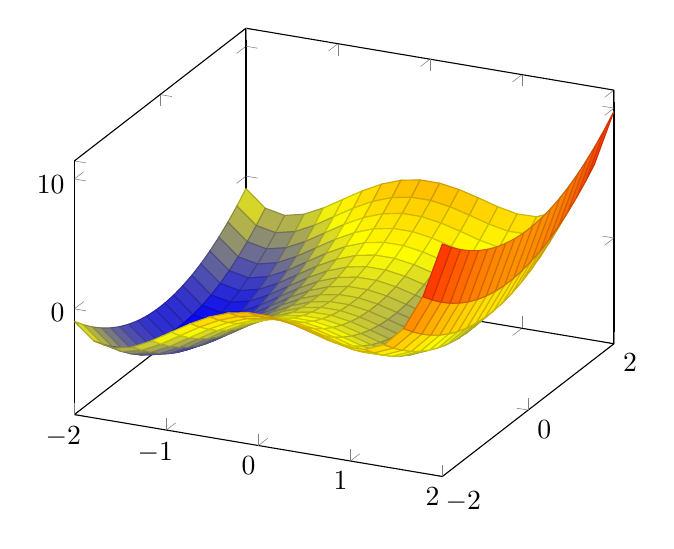
\begin{tikzpicture}
\begin{axis}
 
\addplot3 [
    domain=-2:2,
    domain y = -2:2,
    samples = 20,
    samples y = 20,
    surf] {.9*x^4  + .67*x^3 - 3*x^2 + 2 + y^2 - 4};
 
\end{axis}
 
\end{tikzpicture}
    \end{center}


\begin{motivating}
    What is the multivariable analogue of the first derivative test?
\end{motivating}

\begin{remark}
        Observe that if $\bm{P} \in \R^n$ is a local maxima or minima of $f: \R^n \to \R$, and if $f$ is differentiable at $\bm{P}$, then $Df(\bm{P})$ is the zero linear transformation (equivalently, $\nabla f = \bm{0}$).

        That is, the tangent plane at $\bm{P}$ is parallel to the plane $x_{n+1} = 0$.
    \end{remark}

\begin{definition}
        A point $\bm{P} \in \R^n$ is said to be a \textbf{critical point} of a function $f: \R^n \to \R$ if either

        \begin{enumerate}
            \item $Df(\bm{P}) = 0$, OR
            \item $Df(\bm{P})$ does not exist.
        \end{enumerate}
      
    \end{definition}

\begin{proposition}
     Equivalently, $\bm{P}$ is a critical point of $f: \R^n \to \R$ if
    \begin{enumerate}
            \item $\nabla f(\bm{P}) = \bm{0}$, OR
            \item $\nabla f(\bm{P})$ does not exist.
        \end{enumerate}
\end{proposition}


\begin{theorem}[The multivariable first derivative test]
        If $f: \R^n \to \R$ has a local maximum or minimum at $\bm{P}$, then $\bm{P}$ is a critical point of $f$.
    \end{theorem}


    \begin{remark}
        The converse of the first derivative test does not hold:
        
        If $\bm{P}$ is a critical point of $f$, then $\bm{P}$ is not necessarily a local maximum or minimum.
    \end{remark}

    \begin{example}
        Consider the function $f(x,y) = x^2-y^2$.  Observe that $(0,0)$ is a critical point, but it is neither a local maximum or a minimum.

    \begin{center}
        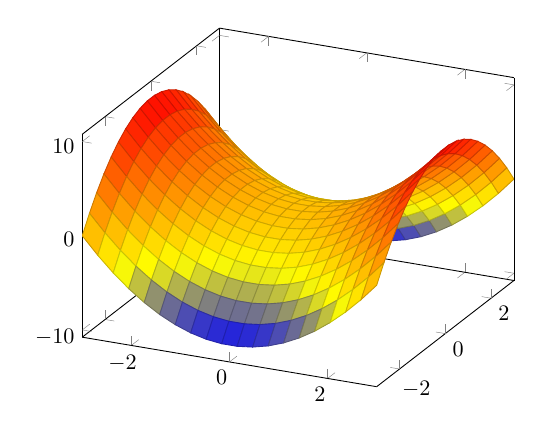
\begin{tikzpicture}[scale=0.8]
 
\begin{axis}
 
\addplot3 [
    domain=-3:3,
    domain y = -3:3,
    samples = 20,
    samples y = 20,
    surf] {x^2 - y^2};
 
\end{axis}
 
\end{tikzpicture}
    \end{center}


    \end{example}

\subsubsection{Classifying local extrema}

\begin{motivating}
    How can we algebraically classify the behavior of critical points?
\end{motivating}

Recall that in single-variable calculus, we can do so using the \textbf{second derivative test}:

\begin{theorem}[The single-variable second derivative test]\label{single2ndderiv}

Let $f : \R \to \R$ be a single variable function.

\begin{enumerate}
    \item If $f'(P) = 0$ and $f''(P) > 0$, then there is a \textbf{local minimum} at $x=P$. 
    \item If $f'(P) = 0$ and $f''(P) < 0$, then there is a \textbf{local maximum} at $x=P$. 
    \item If $f'(P) = 0$ and $f''(P) = 0$, then the test is \textbf{inconclusive}.
\end{enumerate}

If $f''(P)$ does not exist, then the test is \textbf{inconclusive}.

\end{theorem}

\begin{motivating}
    What is the multivariable analogue of the second derivative test?
\end{motivating}

First, we need to figure out what we mean by the second derivative of a multivariable function.

Recall from example \ref{derivlinearmap} that the derivative of a linear transformation $T$ is $T$ itself. That is, 
$$DT(\bm{x_0}) = T$$
Thus, we cannot na\"ively define the second derifative of $f$ as $D(Df(\bm{x_0})$.

\begin{remark}
    We have defined the derivative $Df(\bm{x_0})$ to be the linear approximation of $f$ \textnormal{at a point} $\bm{x_0} \in \R^n$.
    
    This is analogous to finding the slope of the tangent line of a single variable function \textnormal{at a point} $x \in \R$.
    
    \end{remark}

Therefore, we wish to find the derivative of $Df$, not of $Df(\bm{x_0})$, where 
$$Df : \R^n \to M_{1\times n}(\R)$$

However, observe that we have only defined derivatives of functions $f : \R^m \to \R^n$.  We have not defined the derivative of a function that outputs matrices!  However, since we know that $$M_{1\times n}(\R) \cong \R^n$$ via the transpose map $(-)^\intercal$ 
$$M \mapsto M^\intercal$$

We can then consider the map $$(Df)^\intercal : \R^n \cong M_{1\times n}(\R) \to \R^n$$
which sends a vector 
$$\bm{x_0} \mapsto \begin{bmatrix}
D_1f(\bm{x_0}) \\
\vdots \\
D_nf(\bm{x_0})
\end{bmatrix}$$

Observe that $$(Df)^\intercal(\bm{x_0}) =  \nabla f(\bm{x_0})$$  
Thus, we can make the following definition:

\begin{definition}
A multivariable function $f: \R^n \to \R$ is \textbf{twice-differentiable} if $f : \R^n \to \R$ and $\nabla f : \R^n \to \R^n$ are both differentiable.

\vspace{1em}

If $f: \R^n \to \R$ is twice-differentiable, then the \textbf{second derivative of} $f$ \textbf{at} $\bm{x_0}$ is defined as 
$$D^2f(\bm{x_0}) := D(\nabla f)(\bm{x_0})$$
\end{definition}

\begin{definition}
Let $f: \R^n \to \R$ be a twice-differentiable function. Then the standard matrix of $D^2f(\bm{x_0})$ is called the \textbf{Hessian matrix}, 
$$\left[H_f(\bm{x_0})\right]$$
\end{definition}

\begin{proposition}
    The \textbf{Hessian matrix} of $f:\R^n \to \R$ at $\bm{x_0}$ is 
    
    \begin{equation*}
        [H_f(\bm{x_0})] = \begin{bmatrix}
D_1D_1f(\bm{x_0}) & D_2D_1f(\bm{x_0}) & \cdots & D_nD_1f(\bm{x_0}) \\
D_1D_2f(\bm{x_0}) & D_2D_2f(\bm{x_0}) & \cdots & D_nD_2f(\bm{x_0}) \\
\vdots & \vdots & \vdots & \vdots\\
D_1D_nf(\bm{x_0}) & D_2D_nf(\bm{x_0}) & \cdots & D_nD_nf(\bm{x_0}) 
\end{bmatrix}
    \end{equation*}
\end{proposition}

In other words, the Hessian matrix is the $n \times n$ matrix of all second-order partial derivatives of $f$,
    $$f_{x_jx_i} = D_iD_j f = \frac{\partial}{\partial x_i}\left(\frac{\partial f}{\partial x_j}\right)$$


\begin{example}
    Let $f : \R^2 \to \R$ be defined by $f(x,y)= xe^{xy}$.  Compute the partial derivatives, the Jacobian matrix, $\nabla f$, and the Hessian matrix of $f$ at $(1,1)$.
\end{example}

\begin{definition}
        A function $f : U \subset \R^n \to \R$ is said to be of class $C^2$ (writing $f \in C^2(U)$) if all second-order partial derivatives exist and are continuous on $U$.
    \end{definition}


    \begin{definition}
        A function $f : U \subset \R^n \to \R$ is said to be of class $C^k$ (writing $f \in C^k(U)$) if all $k$th-order partial derivatives exist and are continuous on $U$.
    \end{definition}


    \begin{definition}
        A function $f : U \subset \R^n \to \R$ is said to be of class $C^\infty$ (writing $f \in C^\infty(U)$) if \underline{all} partial derivatives exist and are continuous on $U$.
    \end{definition}

\begin{theorem}[Clairaut's theorem]
    
    Let $f: \R^n \to \R$.  Suppose that $D_if$, $D_jf$, and $D_iD_jf$ exist and are continuous on an open disk $D \subset \R^n$.  Then $D_jD_if$ exists on $D$, and moreover
    $$D_iD_j = D_jD_i\ \textnormal{on the disk} \ D$$
    
    \end{theorem}

    Clairaut's theorem is more commonly stated (and easily proved) as the following corollary:
    \begin{corollary}
       Let $f \in C^2(U)$.  Then  $$D_iD_j = D_jD_i\ \textnormal{on the region} \ U$$
    \end{corollary}

\begin{example}
    We can use Clairaut's theorem to compute the partial derivative $g_{zzwx}$ for $$g(x,y,w,z) = x^2w^2z^2 + \sin\left(\frac{xy}{z^2}\right)$$

    Note that as long as $z \neq 0$, we have that all partial derivatives of $g$ exist. Thus, $g_{zzwx} = g_{wxzz}$ as long as $z \neq 0$.  
    
    Observe that $g_w = 2x^2wz^2$.  Thus, $g_{zzwx} = g_{wxzz} = 8wx$, as long as $z\neq 0$
\end{example}

\begin{corollary}
    If $f \in C^2(U)$, then $$\left[H_f(\bm{x_0})\right]^\intercal = \left[H_f(\bm{x_0})\right]$$
\end{corollary}

With the second derivative defined, we can now state the two-variable second derivative test:

\begin{theorem}[The two-variable second derivative test]

Let $\bm{x_0} \subset U$ be a critical point of $f(x,y) : U \to \R$, and suppose that $f \in C^2(U)$.  Let us write $D = \textnormal{det}[H_f(\bm{x_0})]$.

\begin{enumerate}
    \item If $D > 0$ and $f_{xx}(\bm{x_0}) > 0$, then there is a \textbf{local minimum} at $\bm{x_0}$.
    \item If $D > 0$ and $f_{xx}(\bm{x_0}) < 0$, then there is a \textbf{local maximum} at $\bm{x_0}$. 
    \item If $D < 0$, then $f$ has a \textbf{saddle point} at $\bm{x_0}$. 
    \item If $D = 0$, then the test is \textbf{inconclusive}. 
\end{enumerate}

If $D$ does not exist, then the test is \textbf{inconclusive}.
\end{theorem}

\begin{remark}
    At a critical point $P = (a,b)$, we can apply the single-variable second derivative test to
    
    \begin{itemize}
        \item the trace $f(a,y) = g(y)$ in the plane $x=a$
        \item the trace $f(x,b) = h(x)$ in the plane $y=b$
    \end{itemize}

    For the former, observe that 
    
    $$f_{yy}(a,b) = g''(b) \text{ is } \left\{
    \begin{array}{ll}
			> 0  & \text{ if } f(a,y) = g(y) \text{ has a local min at } b \\
			< 0  & \text{ if } f(a,y) = g(y) \text{ has a local max at } b
		\end{array}
		\right.$$

  For the latter, observe that
	$$f_{xx}(a,b) = h''(a) \text{ is } \left\{
		\begin{array}{ll}
			> 0  & \text{ if } f(x,b) = h(x) \text{ has a local min at } a \\
			< 0  & \text{ if } f(x,b) = h(x) \text{ has a local max at } a
		\end{array}
		\right.$$

    \end{remark}



\begin{motivating}
        How does this generalize to multiple variables?
    \end{motivating}

\begin{theorem}[Second order Taylor approximation]
    
    If $f : U \subset \R^n \to \R$ is \underline{differentiable} at a point $\bm{a} \in \R^n$, and $\bm{x}$ is close to $\bm{a}$, then 
    $$f(\bm{x}) \approx f(\bm{a}) + [Df(\bm{a})](\bm{x-a}) + \frac{1}{2}\left([H_f(\bm{a})](\bm{x-a})\right) \cdot (\bm{x-a}) $$
    
    \end{theorem}

\begin{definition}
    Let $A \in M_{n \times n}(\R)$ be a symmetric matrix (that is, $A^\intercal = A$). Then $A$ is said to be
    
    \begin{enumerate}
        \item \textbf{positive definite} , if for all $\bm{x} \neq \bm{0}$, then $(A\bm{x}) \cdot \bm{x} > 0$,
        \item \textbf{negative definite} if for all $\bm{x} \neq \bm{0}$, then $(A\bm{x}) \cdot \bm{x} < 0$,
        \item \textbf{indefinite} otherwise.
    \end{enumerate}
    
    \end{definition}

\begin{theorem}[The multivariable second derivative test]

Let $\bm{x_0} \in U \subset \R^n$ be a critical point of a function $f : U \subset \R^n \to \R$. 

\vspace{.5em}
Suppose that $f \in C^2(U)$, and that the Hessian $[H_f(\bm{x_0})]$ is invertible.

\begin{enumerate}
    \item If $[H_f(\bm{x_0})]$ is positive definite, then there is a \textbf{local minimum} at $\bm{x_0}$.
    \item If $[H_f(\bm{x_0})]$ is negative definite, then there is a \textbf{local maximum} at $\bm{x_0}$. 
    \item If $[H_f(\bm{x_0})]$ is indefinite, then $f$ has a \textbf{saddle point} at $\bm{x_0}$. 
\end{enumerate}

\end{theorem}


\subsection{Global Optimization}

We saw from the previous section that the gradient and the second derivative test allow us to find and classify \textbf{local} maxima and minima.
    
    \begin{motivating}
    (On a given domain), how can we find \textbf{global} maxima and minima?
    \end{motivating}

In single-variable calculus, we have the following theorem:

\begin{theorem}[Single-variable global minima and maxima]
    If $f(x)$ is continuous on a closed and bounded interval $[a,b]$, then $f$ has a global maximum and a minimum on $[a,b]$.
    
    \vspace{1em}
    
    That is, there exists an $M \in [a,b]$ and an $m \in [a,b]$ such that $f(m) \leq f(x) \leq f(M)$ for all $x \in [a,b]$.
    \end{theorem}
    
    
    \begin{theorem}
    The global maxima and minima of $f(x)$ on $[a,b]$ either occur at the critical points of $f$ in $[a,b]$, or on the boundary of $[a,b]$.
    \end{theorem}

    \begin{remark}
    Observe that if $A \subset \R$ is not closed, or not bounded, then global maxima/minima are not guaranteed to exist.
    \end{remark}

    \begin{example}
    The interval $A = [0,1)$ is bounded, but not closed.  
    
    The function $f(x) = x$ has no global maximum in $A$, but has a global minimum at $x=0$.

    The function $f(x) = -x$ has a global maximum at $x=0$, but no global minimum in $A$.
    \end{example}

    \begin{example}
     The interval $A = \{x \ | \ x \geq 0 \}$ is closed, but not bounded.   
        
    The function $f(x) = x$ has no global maximum in $A$, but has a global minimum at $x=0$.

    The function $f(x) = -x$ has a global maximum at $x=0$, but no global minimum in $A$.
    \end{example}

    
    \begin{example}
     The interval $A = \{x \ | \ x > 0 \}$ is neither closed nor bounded.   
        
    The function $f(x) = x$ has no global maximum or minimum in $A$.

    The function $f(x) = \sin(x)$ has (infinitely many) global maxima and minima in $A$.
    \end{example}

Thus, we have a few questions to consider:

    \begin{motivating}
How do we generalize the notion of a bounded and closed interval $[a,b] \subset \R$ to a subset $A \subset \R^n$?
\end{motivating}

\begin{motivating}
    Can we find the possible points where global maxima/minima occur?
\end{motivating}

To answer the first question, we will need to define the notions of bounded and closed sets in $\R^n$.

\begin{definition}
A subset $D \subset \R^n$ is \textbf{bounded}\define{bounded set} if there exists some $r > 0$ such that $D \subset B_r(\bm{0})$.
\end{definition}

\begin{definition}
A point $\bm{x_0} \in \R^n$ is a \textbf{boundary point}\define{boundary point} of $D \subset \R^n$ if: for all $\varepsilon > 0$,

\begin{enumerate}
    \item $B_\varepsilon(\bm{x_0}) \cap D$ is non-empty, \textbf{and}
    \item $B_\varepsilon(\bm{x_0}) \cap D^{c}$ is non-empty.
\end{enumerate}

\end{definition}

\begin{definition}
    A subset $D \subset \R^n$ is \textbf{closed}\define{closed set} if it contains all of its boundary points.
        
    \end{definition}

\begin{example}
    Consider the set $$D = \{(x,y) \in \R^2 \ | \ x \geq 0, y \geq 0\}$$   
    
    The boundary of $D$ is the set $$\{(x,0) \in \R^2 \ | \ x \geq 0\} \ \bigcup \ \{(0,y) \in \R^2 \ | \ y \geq 0\}$$
    $D$ is closed, but not bounded.
\end{example}

\begin{example}
    Consider the set $$D = \{(x,y) \in \R^2 \ | \ 1 < (x-a)^2 + (y-b)^2  \leq 3 \}$$ is bounded, but not closed.
    
    The boundary of $D$ is the set $$\{(x,y) \in \R^2 \ | \  (x-a)^2 + (y-b)^2 =1 \} \ \bigcup \ \{(x,y) \in \R^2 \ | \ (x-a)^2 + (y-b)^2 = 3 \}$$
    $D$ is bounded, but not closed.
\end{example}

If a region $D$ is closed and bounded, then we can guarantee the existence of global maxima and minima for a continuous function on $D$:

\begin{theorem}[Multivariable global minima and maxima]
    If $D$ is a closed and bounded subset of $\R^n$, and $f$ is a continuous function on $D$, then $f$ 
    has a global maximum and a global minimum in $D$.
    
    \vspace{1em}
    
    That is, there exists an $\bm{M} \in D$ and an $\bm{m} \in D$ such that $f(\bm{m}) \leq f(\bm{x}) \leq f(\bm{M})$ for all $\bm{x} \in D$.
    \end{theorem}

    \begin{theorem}
    The global maxima and minima of $f$ on $D$ either occur at the critical points of $f$ in $D$, or on the boundary of $D$.
    \end{theorem}

    We know how to use the gradient and the second derivative test allow us to find and classify \textbf{local} maxima and minima.  The question we turn to now is how to find maxima and minima on the boundary of a region $D$:

\subsection{Constrained optimization}

    \begin{motivating}
        Given a region $D$, how can we find the maxima and minima on $D$?
    \end{motivating}

\begin{remark}
    The boundary of $D \subset \R^2$ can be thought of as:
    
    \begin{itemize}
        \item the parametric curve corresponding to $\bm{r}(t) = \langle x(t),y(t) \rangle$.
        \item The $z=0$ trace of a graph $z = g(x,y)$
    \end{itemize}
    
    \end{remark}

    To find local maxima and minima of $f(x,y)$ on the boundary of $D$, we are trying to find the local maxima and minima of $f(x,y)$ subject to the condition $g(x,y) = 0$.  
    In other words, we are trying to optimize $f(x,y)$ given the constraint $g(x,y) = 0$.  We can do so using the method of Lagrange multipliers:
    
    \begin{theorem}[The method of Lagrange Multipliers]
    Assume that $f(x,y)$ and $g(x,y)$ are differentiable functions.  If 
    \begin{enumerate}
        \item  $f(x,y)$ has a local maximum or minimum subject to the constraint $g(x,y)=0$ at a point $(a,b)$, \textbf{AND}
        \item if $\nabla g(a,b) \neq 0$
    \end{enumerate}
    
    then there is a scalar $\lambda$ such that 
    $$\nabla f(a,b) = \lambda \nabla g(a,b)$$
    \end{theorem}

    \begin{corollary}
    We can use the \textbf{Lagrange equations} 
    $$f_x(a,b) = \lambda g_x(a,b) \qquad \textnormal{and} \qquad f_y(a,b) = \lambda g_y(a,b)$$
    to determine the critical points on the boundary.
    \end{corollary}
    
    \begin{definition}
    Points $P = (a,b)$ that satisfy the Lagrange equations for the optimization problem of $f(x,y)$ with constraint $g(x,y) = 0$ are called \textbf{critical points for optimization with constraint}.
    \end{definition}

    \begin{remark}
    A constrained critical point is not necessarily a local max or a local min.
    \end{remark}

    \begin{example}
    Maximize the area of a rectangular fence subject to the constraint that the perimeter is equal to 20.
    \end{example}

    \begin{example}
    Maximize $f(x,y) = xy$ subject to the constraint $4x^2 + 9y^2 = 32$.    
    \end{example}

    \subsubsection{Classifying constrained extrema}

    \begin{motivating}
    How can we tell if the Lagrange multiplier method give us a local max? a local min?    
    \end{motivating}


    We need an analogue of the second-derivative test for constrained optimization:

    \begin{definition}
    Assume that $f, g : \R^2 \to \R$ are differentiable functions.  Suppose that we are trying to optimize $f(x,y)$ subject to the constraint $g(x,y) = 0$.

    Then the \textbf{Lagrange function} is a function $\Lambda : \R^3 \to \R$ defined as 
    $$\Lambda(x, y, \lambda) := f(x,y) + \lambda g(x,y)$$
    
    \end{definition}

    \begin{definition}
    The \textbf{bordered Hessian matrix} $[H_\Lambda]$ is the Hessian matrix of the Lagrange function $\Lambda(x, y, \lambda)= f(x,y) + \lambda g(x,y)$:

    \begin{align*}
        [H_\Lambda] &= \begin{bmatrix}
D_xD_x \Lambda & D_yD_x \Lambda  & D_\lambda D_x \Lambda \\
D_xD_y \Lambda & D_yD_y \Lambda  & D_\lambda D_y \Lambda \\
D_xD_\lambda  \Lambda & D_yD_\lambda  \Lambda & D_\lambda D_\lambda \Lambda 
\end{bmatrix} \\ 
&= \left[\begin{array}{@{}cc|c@{}}
f_{xx} + \lambda g_{xx} & f_{xy} + \lambda g_{xy}  & g_x \\
f_{yx} + \lambda g_{yx} & f_{yy} + \lambda g_{yy}  & g_y \\
\hline
g_x & g_y  & 0
\end{array}\right] \\
&= \left[\begin{array}{@{}c|c@{}}
 H_{\Lambda(x,y)}  & [J_{g(x,y)}]^\intercal \\
\hline
J_{g(x,y)} & 0 
\end{array}\right]
    \end{align*}
    
\end{definition}

\begin{theorem}
    Assume that $f, g : \R^2 \to \R$ are differentiable functions.  Suppose that we are trying to optimize $f(x,y)$ subject to the constraint $g(x,y) = 0$.

    Let $\bm{x_0}$ be a constrained critical point, with associated Lagrange multiplier $\lambda_0$.  Let us write $|\overline{H}| = \textnormal{det}[H_\Lambda(\bm{x_0}, \lambda_0)]$.

    \begin{enumerate}
    \item If $|\overline{H}| > 0$ then there is a \textbf{local maximum} at $\bm{x_0}$.
    \item If $|\overline{H}| < 0$, then $f$ has a \textbf{local minimum} at $\bm{x_0}$. 
    \item If $|\overline{H}| = 0$, then the test is \textbf{inconclusive}. 
\end{enumerate}
    \end{theorem}


\subsection{Exercises}


\begin{problem}{clairaut1}
    Consider the function $$f(x,y,z,w) = \frac{3x^2 + e^yz + x}{3y^2+2e^{w^2}}$$ 

Compute the fourth order partial derivative $f_{wyzx}$.
\end{problem}

\begin{problem}{opt1}
    Consider the function $$f(x,y) = x^3 - xy +  y^3 $$
    
    Find the critical points of $f$, and use the second derivative test to classify the critical points of $f$.
\end{problem}

\begin{problem}{opt2}
    Consider the function $$f(x,y) = x^2 + y^3 - 2x - 6y$$
    
    Find the critical points of $f$, and use the second derivative test to classify the critical points of $f$.
\end{problem}

\begin{problem}{opt3}
    Consider the function $$f(x,y) = \ln(x) + 2\ln(y) -x - 4y$$
    
    Find the critical points of $f$, and use the second derivative test to classify the critical points of $f$.
\end{problem}

\begin{problem}{closedbounded1}
    Is the set $$D = \{(x,y) \in \R^2 \ | \ 0 \leq x + y \leq 1 \}$$ closed? bounded? What is it's boundary?
\end{problem}

\begin{problem}{closedbounded2}
    Is the set $A = \{(x,y) \ | \ -1 < x \leq 1, -1 \leq y < 1\}$ closed? bounded? What is it's boundary?
\end{problem}


\begin{problem}{constrainedopt1}
    Find the critical points of $f(x,y) = x^4 + y^4$ subject to the constraint $x^2+y^2=1$.  
\end{problem}

\begin{problem}{global1}
    Determine the coordinates of the global maxima and minima of $f(x,y) = x^4 + y^4$ on the disk $D = \{ (x,y) \ | \ x^2 + y^2 \leq 1\}$.
\end{problem}

\begin{problem}{constrainedopt2}
    Find the critical points of $f(x,y) = -x^2+2y^2+6x$ subject to the constraint $x^2+y^2=1$.  
\end{problem}

\begin{problem}{global2}
    Determine the coordinates of the global maxima and minima of $f(x,y) = -x^2+2y^2+6x$ on the disk $D = \{ (x,y) \ | \ x^2 + y^2 \leq 1\}$.
\end{problem}

\begin{problem}{constrainedsquare}
    Let $f(x,y) = (x^3 - 3x) + (y^3-3y)$.  Find the constrained critical points of $f(x,y)$ on the boundary of the region $S = \{(x,y) \ | -1 \leq x \leq 1, -1 \leq y \leq 1\}$
\end{problem}

\begin{problem}{globalsquare}
    Let $f(x,y) = (x^3 - 3x) + (y^3-3y)$.  Find the global maxima and minima of $f(x,y)$ on the region $S = \{(x,y) \ | -1 \leq x \leq 1, -1 \leq y \leq 1\}$
\end{problem}

\begin{problem}{noglobalmax}
    Find a continuous function that does not have a global maximum on the domain $$D = \{(x,y) \in \R^2 \ | \ 0 \leq x + y \leq 1 \}$$
\end{problem}


\begin{problem}{constrainedopt3}
    Find the critical points of $f(x,y) = 4x^2+9y^2$ subject to the constraint $xy=4$.  
\end{problem}

\begin{problem}{closesttoline}

Find the point $(a,b)$ on the line $4x+9y=12$ that is closest to the origin.
   
\end{problem}

\begin{problem}{closesttoplane}

Find the point $\bm{x_0}=(x_0,y_0,z_0)$ on the plane $ax + by + cz = d$ that is closest to the origin.  What is the distance from $\bm{x_0}=(x_0,y_0,z_0)$ to the origin?
   
\end{problem}

\chapter{Integration on $\R^n$}

 \begin{motivating}
    What is the definition of the integral in single variable calculus? 
    \end{motivating}
    

\section{Defining the integral}

\begin{motivating}
    What is the definition of the integral in single variable calculus? 
\end{motivating}

PICTURE

    \begin{enumerate}
        \item Can we define the integral such that we can deal with both  $\int_\infty^\infty f(x) \ dx$ and $\int_a^b f(x) \ dx$?
        \item Can we define the integral in a way that easily generalizes to multivariable functions $f: \R^n \to \R$?
        \item What kinds of functions can we integrate? 
    \end{enumerate}

In these lecture notes, we'll be dealing with proper/definite integrals.  That is, we will want our integrals to have finite values.\footnote{It takes some care to define non-proper integrals in multivariable calculus!}

That is, we'll be working with functions that are \textbf{bounded} with \textbf{bounded support}.

\begin{definition}
A subset $D \subset \R^n$ is \textbf{bounded} if there exists some $r > 0$ such that $D \subset B_r(\bm{0})$.
\end{definition}

\fixthis{recall}
    
    
    \begin{definition}
    A function $f: A \subset \R^n \to \R$ is \textbf{bounded}\define{bounded function} if its image $$\{f(\bm{x}) \ | \ \bm{x} \in A \}$$ is a bounded subset of $\R$.
    \end{definition}

\fixthis{recall}

\begin{definition}
A point $\bm{x} \in \R^n$ is a \textbf{boundary point} of $D \subset \R^n$ if: for all $\varepsilon > 0$,

\begin{enumerate}
    \item $B_\varepsilon(\bm{x}) \cap D$ is non-empty, \textbf{and}
    \item $B_\varepsilon(\bm{x}) \cap D^{c}$ is non-empty.
\end{enumerate}
\end{definition}
    
    \begin{definition}
    The \textbf{closure} of a set $D \subset \R^n$ is the union of $D$ and the boundary of $D$.  That is, the closure is the set $$\overline{D} = \{\bm{x} \in \R^n \ | \ B_r(\bm{x}) \cap D \neq \varnothing \textnormal{ for all } r\in\R \}$$  
    \end{definition}

\begin{proposition}
    A set $D$ is closed (\fixthis{recall}) if and only if $$D = \overline{D}$$
\end{proposition}

\begin{definition}
    The \textbf{set of non-zero values of a function} $f : A \subset \R^n$ is the set $$\{\bm{x} \in A \ | \ f(\bm{x}) \neq 0\}$$
\end{definition}

\begin{definition}
    The \textbf{support}\define{support of a function} of a function $f : A \subset \R^n \to \R$ is the \textbf{closure} of the set of non-zero values of a function:
    $$\textnormal{supp}(f) := \overline{\{\bm{x} \in A \ | \ f(\bm{x}) \neq 0\}}$$

\begin{center}
    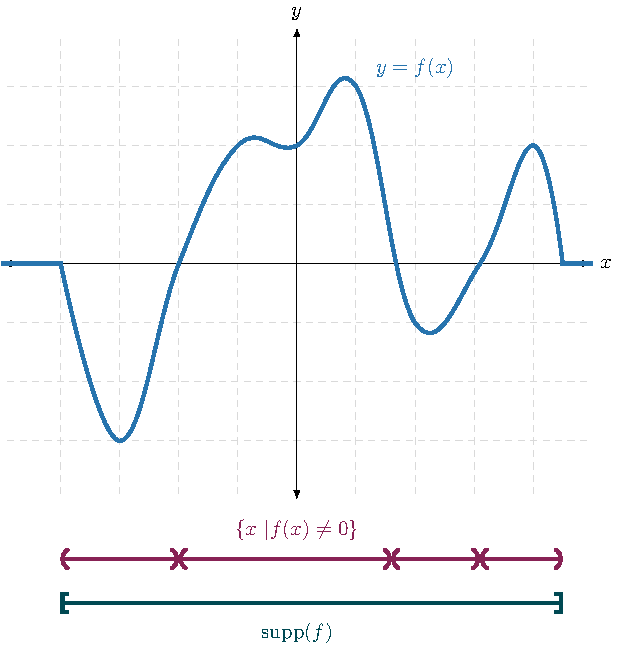
\includegraphics{chapters/4-IntegrationRn/figures/figures-supportpic.pdf}
\end{center}

\end{definition}

\begin{definition}
    A function has \textbf{bounded support}\define{bounded support} if its support is bounded.  

    Equivalently, there exists $R>0$ such that $f(\bm{x}) = 0$ for all $||\bm{x}|| > R$.
    \end{definition}

\begin{example}
    The function $f(x) = \sin(x)$ does not have bounded support.  In fact, the set of non-zero points of $\sin(x)$ is the set
    $$\{x \in \R \ | \ x \neq n\pi \}$$
    This set is already unbounded, and when we take the closure, $\textnormal{supp}(f) = \R$.  
    
    However, the function $$g(x) = \left\{
		\begin{array}{ll}
			\sin(x) & \text{ if } -\pi \leq x \leq \pi \\
			0 & \text{ otherwise}
		\end{array}
		\right.$$
  has bounded support.  The set of non-zero points of $g(x)$ is the set
    $$(-\pi,0) \cup (0,\pi)$$
  When we take the closure, $\textnormal{supp}(f) = [-\pi,\pi]$, which is bounded.  
    

  
\end{example}

We can now define the notion of multivariable integral for bounded functions with bounded support.  


\subsection{Integration over $\R^n$}

The main idea of integrating a function $f: \R^n \to \R$ is not so difficult: 

\begin{enumerate}
    \item We chop up our region into pieces.
    \item We sample $f$ on each of the pieces, and sum over the pieces.
    \item We take the limit of the sum as the size of the pieces shrinks.
\end{enumerate}

However, \textbf{we will need to be careful}, as we will encounter some technical difficulties in making these ideas rigorous.


We will begin with chopping up the domain of $f$ (e.g. $\R^n$) into pieces.  In technical terms, we will construct a \textbf{partition} of $\R^n$.

\begin{definition}
    A \textbf{partition} of a set $X$ is a collection of non-empty subsets $X_\alpha \subset X$ such that every elemnent of $x \in X$ is in \textbf{exactly one} $X_\alpha$.
\end{definition}

\begin{definition}
    Given a vector $\bm{k} = \langle k_1, \cdots, k_n\rangle \in \Z^n \subset \R^n$ (that is, $k_i \in \Z$ for all $i$), we can define the \textbf{dyadic cube} $C_{\bm{k},N}$ in $\R^n$ as
    $$C_{\bm{k},N} := \left\{ \bm{x} = \langle x_1, \cdots, x_n\rangle \in \R^n \ | \ \frac{k_i}{2^N} \leq x_i < \frac{k_i+1}{2^N}\right\}$$
    
    \end{definition}

\begin{example}

        What is the dyadic cube $C_{1,1}$ in $\R^1$?
        
        What is the dyadic cube $C_{1,2}$ in $\R^1$?
    

\fixthis{picture}
    
        What is the dyadic cube $C_{\langle1,1\rangle,1}$ in $\R^2$?

\end{example}





\begin{proposition}
    The volume of a dyadic cube $C_{\bm{k},N}$ in $\R^n$ is $\frac{1}{2^{Nn}}$.
    \end{proposition}

\begin{proposition}
    For a fixed $N$, the collection of all dyadic cubes $$D_N(\bm{\R^n}) := \left\{C_{\bm{k},N} \ | \ \textnormal{for all} \ \bm{k} \in \Z^n \right\}$$ partitions $\R^n$. We call $D_N(\bm{\R^n})$ the $N$\textbf{-th dyadic partition of} $\R^n$.
    \end{proposition}





The dyadic partition is a convenient choice of \textbf{partition} of $\R^n$. We have chosen this particular partition as it is systematic and easy to define.

There are many other ways to partition $\R^n$, and they each lead to an equivalent definition of the multivariable integral.  For example, it turns out that the partitions do not need to be uniform (e.g. we could take rectangles with differing widths).  Moreover, we could take partitions depending on the range of the function (this leads to the notion of the Lebesgue integral).

 


Given our dyadic cube partition, we now turn to sampling points from the partition:

\fixthis{lower left corner, midpoint, etc.}

\begin{definition}\label{def:riemannsum}
    Given a choice of $\bm{x_{k,N}} \in C_{\bm{k},N}$ for every cube, the $N$-th \textbf{Riemann sum}\define{Riemann sum} is defined as 
    $$R_N(f) := \sum_{C \in D_N(\R^n)} f(\bm{x_{k,N}}) \ \textnormal{vol(C)}$$
    \end{definition}

We have many choices for sampling points, and it is a priori unclear that these various sampling methods should produce the same value for our integral when we take the limit as $N$ goes to $\infty$.

Thus, we will use Darboux sums to define the multivariable integral - this will guarantee that if the limit as $N$ goes to $\infty$ exists, then any sampling method will produce the same value\footnote{See proposition \ref{prop:riemannisintegrable} and exercise \ref{problem:riemannintegrabletodarboux}}.

 \begin{definition}
    Let $X \subset \R$.  A number $M \in \R$ is an \textbf{upper bound of $X$}\define{upper bound} if for every $x \in X$, we have that $x \leq M$.  
 
    \end{definition}

\begin{definition}   
    Let $q$ be an upper bound of $X$. We say $q$ is the \textbf{supremum of $X$}\define{supremum} (or \textbf{least upper bound of $X$}\define{least upper bound}) if for all upper bounds $M$ of $X$, we have that $q \leq M$.
    
    We write $q := \sup(X)$.  If $X$ is not bounded above, we write $\sup(X) = \infty$.
    
    \end{definition}

\begin{definition}
    Let $X \subset \R$.  A number $m \in \R$ is an \textbf{lower bound of $X$}\define{lower bound} if for every $x \in X$, we have that $m \leq x$.  
 
    \end{definition}

\begin{definition}
    Let $p$ be a lower bound of $X$. We say $p$ is the \textbf{infimum of $X$}\define{infimum} (or \textbf{greatest lower bound of $X$}\define{greatest lower  bound} ) if for all lower bounds $m$ of $X$, we have that $m \leq p$.
    
    We write $p := \inf(X)$.  If $X$ is not bounded below, we write $\inf(X) = -\infty$.
    
    \end{definition}

    
    \begin{example}
        Consider the set $X = \{\frac{1}{n} \ | \ n \in \N \}$.  What is $\sup(X)$ and  $\inf(X)$?
    \end{example}

    We would often like to describe the largest and smallest element of a subset of $\R$.  However, if we consider sets like $X = \{1-\frac{1}{n} \ | \ n \in \N \}$ and $Y = \{\frac{1}{n} \ | \ n \in \N \}$, we see immediately that there is no largest elemnt in $X$, and that there is no smallest in $Y$.  Thus, we need to use the notions of the supremum and infimum, instead.


    

    \begin{theorem}[Completeness of $\R$]\label{thm:completness}
    Every nonempty subset $X \subset \R$ has a supremum and infimum. Moreover, $\sup(X)$ and $\inf(X)$ are unique.
    \end{theorem}



    \begin{definition}
    Let $f: \R^n \to \R$ be a function, and $D \subset \R^n$ an arbitrary subset. We will consider the following quantities:
    $$M_D(f) := \sup(\{f(\bm{x}) \ | \ \bm{x} \in D\}) \qquad m_D(f) := \inf(\{f(\bm{x}) \ | \ \bm{x} \in D\})$$
    
    \end{definition}

    \begin{example}
        Consider the subset $C_{1,2}$ in $\R^1$, and let $f(x) = \frac{1}{x}$.  
        
        Calculate $M_{C_{1,2}}(f)$ and $m_{C_{1,2}}(f)$.
    \end{example}


    
    \begin{definition}
    Let $f: \R^n \to \R$ be a bounded function with bounded support. The $N$\textbf{-th upper Darboux sum} and $N$\textbf{-th lower Darboux sum} $f$ are defined as 
    $$U_N(f) := \sum_{C \in D_N(\R^n)} M_C(f)\textnormal{vol(C)} \qquad L_N(f) := \sum_{C \in D_N(\R^n)} m_C(f)\textnormal{vol(C)}$$
    
    \end{definition}

    \begin{center}
        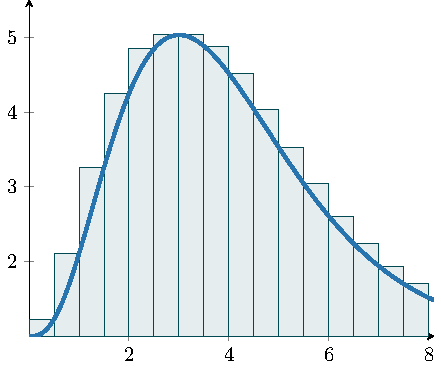
\includegraphics{chapters/4-IntegrationRn/figures/figures-upperdarboux.pdf}
        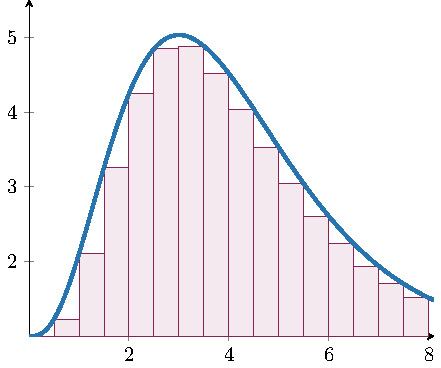
\includegraphics{chapters/4-IntegrationRn/figures/figures-lowerdarboux.pdf}
    \end{center}

    \begin{proposition}
    $$U_N(f) := \frac{1}{2^{Nn}} \sum_{C \in D_N(\R^n)} M_C(f)  \qquad L_N(f) := \frac{1}{2^{Nn}}\sum_{C \in D_N(\R^n)} m_C(f)$$
    \end{proposition}
    
    \begin{proposition}\label{darbouxmonotone}
    As $N$ increases, $U_N(f)$ decreases and $L_N(f)$ increases.
    \end{proposition}

    \begin{center}
        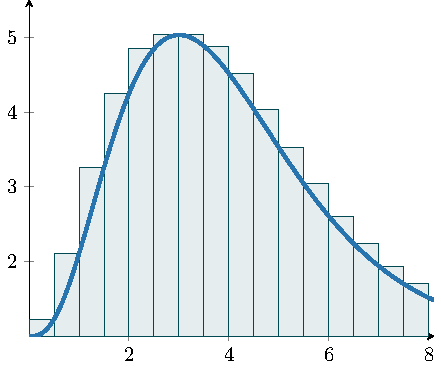
\includegraphics{chapters/4-IntegrationRn/figures/figures-upperdarboux.pdf}
        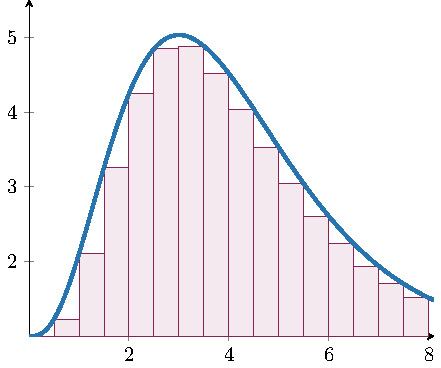
\includegraphics{chapters/4-IntegrationRn/figures/figures-lowerdarboux.pdf}
    \end{center}

    \begin{center}
        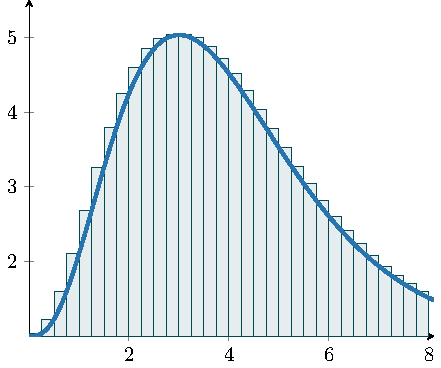
\includegraphics{chapters/4-IntegrationRn/figures/figures-upper2.pdf}
        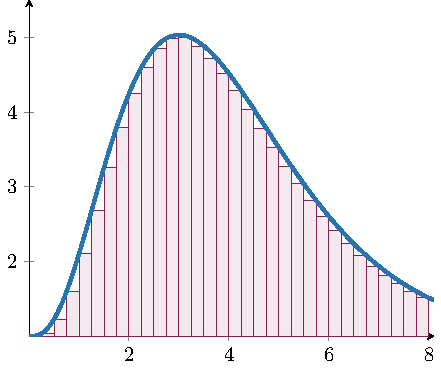
\includegraphics{chapters/4-IntegrationRn/figures/figures-lower2.pdf}
    \end{center}
    
    
    \begin{definition}
    Let $f: \R^n \to \R$ be a bounded function with bounded support.  The \textbf{upper Darboux integral} and \textbf{lower Darboux integral} of $f$ are defined as
    $$U(f) := \lim_{N \to \infty} U_N(f)   \qquad L(f) := \lim_{N \to \infty} L_N(f)$$
    \end{definition}

    \begin{remark}
        \fixthis{limits exist}
    \end{remark}

\begin{definition}\label{def:integrable}
    Let $f: \R^n \to \R$ be a bounded function with bounded support.
    We say that $f$ is \textbf{integrable}\define{integrable} if $U(f) = L(f)$.
    
    The \textbf{integral} of $f$ is $$\int_{\R^n} f(\bm{x}) \ dV := U(f) = L(f)$$

    By proposition \ref{epsilonenough}, this equivalent to asking that for any $\varepsilon > 0$,
    there exists $N$ such that $|U_N(f) - L_N(f)| < \varepsilon$
    \end{definition}

    

    
    \begin{corollary}
    If $f$ is integrable, we can use $U_N(f)$ or $L_N(f)$ to estimate $\int_{\R^n} f(\bm{x}) \ dV$. 
    \end{corollary}


\begin{motivating}
    How should we interpret our definition of the integral?
\end{motivating}

\begin{remark}
    If $f(\bm{x})$ is positive, then the integral is the $n$-dimensional volume under the graph of $f(\bm{x})$.  Otherwise, we can think of the integral as being the \textbf{signed} volume under the graph of $f(\bm{x})$.

    \begin{center}
        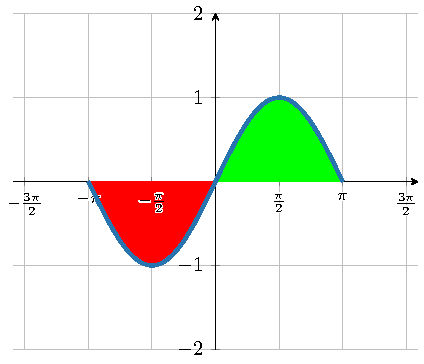
\includegraphics{chapters/4-IntegrationRn/figures/figures-signedvolume.pdf}
    \end{center}
\end{remark}

\begin{motivating}
    What functions are integrable?
\end{motivating}

    \begin{example}
    \begin{theorem}
     If $f : \R^n \to \R$ is a continuous function that is bounded with bounded support, then $f$ is integrable.   
    \end{theorem}

    \fixthis{PICTURE}
    \end{example}

    
However, there are some functions that are ``obviously" integrable, yet are not continuous:

\begin{example}
    Consider the unit square $A = [0,1] \times [0,1] \subset \R^2$.   We can define an indicator function to be the function $1_A  :\R^n \to \R$ is the function 
    $$1_A(\bm{x}) := \left\{
		\begin{array}{ll}
			1 & \text{ if } \bm{x} \in A \\
			0 & \text{ if } \bm{x} \notin A
		\end{array}
		\right.$$

  We expect the integral of $1_A(\bm{x})$ to give us the area of $A$.  However, this function is not continuous.
\end{example}
    
    In section \ref{sec:integrability}, we will discuss criteria for a function $f$ to be integrable.  For now, whenever we say integrable, you should think of continuous functions that are bounded with bounded support.



\begin{remark}
Note that if the integral $\int_{\R^n} f \ dV$ exists, then these two boundedness conditions($f$ is bounded and $f$ has bounded support) guarantee that the integral is finite.    
\end{remark}



\begin{remark}
    Using the Darboux formulation, it follows that if $f$ is integrable, then any choice of sampling  \fixthis{will result in the same value for the integral}
\end{remark}

\begin{definition}
    Recall that given a choice of $\bm{x_{k,N}} \in C_{\bm{k},N}$ for every cube, the $N$-th \textbf{Riemann sum}\define{Riemann sum} is defined as 
    $$R_N(f) := \sum_{C \in D_N(\R^n)} f(\bm{x_{k,N}}) \ \textnormal{vol(C)}$$
    This yields the \textbf{Riemann integral}
    $$\lim_{N \to \infty} R_N(f) = \int_{\R^n} f(\bm{x}) \ dV$$
\end{definition}


    \begin{example}
        For example, we can choose the \textbf{midpoint rule} by choosing $$\bm{x_{k,N}} = \langle \frac{2k_1 + 1}{2^{N+1}}, \cdots, \frac{2k_n + 1}{2^{N+1}} \rangle $$

        \begin{center}
            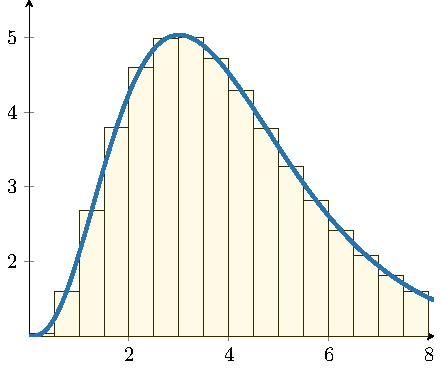
\includegraphics{chapters/4-IntegrationRn/figures/figures-riemannmidpoint.pdf}
        \end{center}
    \end{example}


    
    \begin{example}
     \textbf{Warning!} This only works if you know $f$ is integrable.  The Riemann sum may converge even if the function is not integrable.  Consider the function: $$f(x) := \left\{
		\begin{array}{ll}
			1 & \text{ if } x \in [0,1] \text{ and }  x \notin \Q \\
			0 & \text{ otherwise}
		\end{array}
		\right.$$   
    \end{example}

\begin{proposition}\label{prop:riemannisintegrable}
    If $f: \R^n \to \R$ is integrable, then the integral is the limit of the Riemann sum.  
    \end{proposition}

    \begin{proof}
        Observe that for all cubes $C$, $$M_C(f) \geq f(\bm{x_{k,N}}) \geq m_C(f)$$
        Thus, $$U_N(f) \geq R_N(f) \geq L_N(f)$$
        If $f: \R^n \to \R$ is integrable, by the squeeze theorem, $\lim_{N \to \infty} R_N(f) = \int_{\R^n} f(\bm{x}) \ dV$
    \end{proof}

\subsection{Integration over subsets of $\R^n$}

Observe that we have defined the analogue of $\int_{-\infty}^\infty f(x) \ dx$ in single variable calculus.

    \begin{motivating}
        How can we define the analogue of $\int_a^b f(x) \ dx$?  
    \end{motivating}

    In other words, how do we integrate over sub-regions of $\R^n$?

    Suppose that $B \subset \R^n$ is a region in $\R^n$.  We have two potential ways to define the integral of $f$ over $B$ (denoted $\int_B f \ dV$).  We can either:

    \begin{enumerate}
        \item incorporate $B$ into the definition of the integral $\int_B f \ dV$.        
    In other words, given any subset $B$, we would need to partition $B$ into smaller subsets, and take a limit.
        \item or we can treat $B$ as part of the \textbf{input} of the integral.
        That is, we can use the partition of $\R^n$ that we constructed previously to yield a partition of $B$.
        
    \end{enumerate}

    We will take the second perspective, and define the integral of $f$ over $B$ in terms of some integral $\int_{\R^n} g \ dV$.  We can do so using \textbf{indicator functions}:

    \begin{definition}
    Let $B \subset \R^n$ be a subset.  The \textbf{indicator function} $1_B  :\R^n \to \R$ is the function 
    $$1_B(\bm{x}) := \left\{
		\begin{array}{ll}
			1 & \text{ if } \bm{x} \in B \\
			0 & \text{ if } \bm{x} \notin B
		\end{array}
		\right.$$
    
    \end{definition}

    Observe that given a function $f: \R^n \to \R$, then the function $f(\bm{x})1_B(\bm{x})$ is the piecewise function
    $$f(\bm{x})1_B(\bm{x}) := \left\{
		\begin{array}{ll}
			f(\bm{x}) & \text{ if } \bm{x} \in B \\
			0 & \text{ if } \bm{x} \notin B
		\end{array}
		\right.$$

    This construction restricts the support of $f$ to the region $B$.  Thus, to integrate a function $f: \R^n \to \R$ over $B$, it is equivalent to integrate the function $f(\bm{x})1_B(\bm{x})$ instead.

    \begin{definition}
     Let $B \subset \R^n$, and let $f : \R^n \to \R$ be an integrable function.  Then we can define the \textbf{integral of $f$ over the region $B$} (denoted $\int_B f(\bm{x}) \ dV$ )   as

    $$\int_B f(\bm{x}) \ dV := \int_{\R^n} f(\bm{x})1_B(\bm{x}) \ dV$$
     
    \end{definition}
    
    \fixthis{picture}

    \begin{definition}
    Let $A \subset \R^n$.  If $1_A : \R^n \to \R$ is integrable, then the $n$\textbf{-dimensional volume}\define{n-dimensional volume} of $A$ is $$\textnormal{vol}_n(A) := \int_{\R^n} 1_A \ dV$$
    \end{definition}

    \begin{example}
        Let $A = [0,1] \times [0,1]$ be the unit square  in $\R^2$.  Then the 2-dimensional volume of $A$ (a.k.a the area of $A$) is 1.
    \end{example}

    \begin{example}
        Recall definition \ref{def:graph}, which defines the \textbf{graph of $f : \R^n \to \R$} to be the following subset of $\R^{n+1}$:        
$$\Gamma_f := \{(x_1,\cdots, x_n,f(x_1, \cdots, x_n)) \} \subset \R^{n+1}$$ 
In other words, the graph is given by the equation $$x_{n+1} = f(x_1, \cdots, x_n)$$ in $\R^{n+1}$.

\begin{theorem}\label{thm:graphvolume0}
If $X \subset \R^n$ is a closed and bounded (compact) region, and $f : X \to \R$ be a continuous function, then the ($n+1$)-dimensional volume of the graph $\Gamma_f$ is 0.
\end{theorem}

\begin{center}
    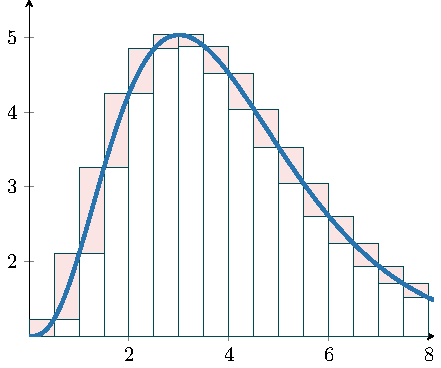
\includegraphics{chapters/4-IntegrationRn/figures/figures-integraloscillation.pdf}
    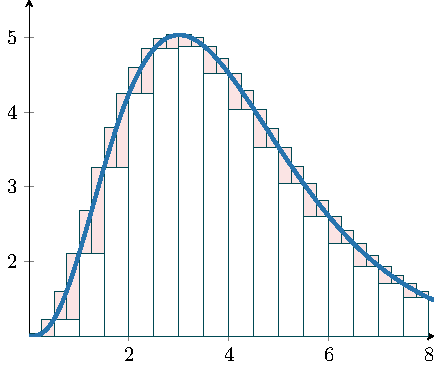
\includegraphics{chapters/4-IntegrationRn/figures/figures-integraloscillation2.pdf}
\end{center}

    \end{example}


    Moreover, we can also use indicator functions to integrate functions that are not defined on all of $\R^n$!  

    \begin{example}
        $f(x) = e^{-\frac{1}{\sqrt{1-x^2}}}$
    \end{example}

    \begin{example}
        Consider the function $f(x) = \frac{1}{\sqrt{1-x^2}}$, which is only defined on $(-1,1)$.

        \begin{center}
            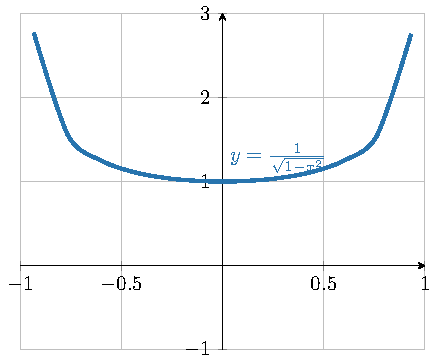
\includegraphics{chapters/4-IntegrationRn/figures/figures-undefinedonr.pdf}
        \end{center}
        Recall that $\int_{-1}^1 \frac{1}{\sqrt{1-x^2}} \ dx = \left[\arcsin{x}\right] \bigg|_{-1}^1 = \pi$.
    \end{example}

Thinking of the integral as the signed volume under the graph, we should expect $$\int_\R \frac{1}{\sqrt{1-x^2}} \ dx = \int_{-1}^1 \frac{1}{\sqrt{1-x^2}} \ dx = \pi$$

    We can make this precise using indicator functions!  

    \begin{definition}
     Let $A \subset \R^n$, and let $f : A \to \R$ be a function. We can extend $f$ to a function $\Tilde{f}(\bm{x}) : \R^n \to \R$ by defining
    $$\Tilde{f}(\bm{x}) := \left\{
		\begin{array}{ll}
			f(\bm{x}) & \text{ if } \bm{x} \in A \\
			0 & \text{ if } \bm{x} \notin A
		\end{array}
		\right.$$
        
    We will often use the following abusive notation when we want to indicate the domain $A$:
    $$f(\bm{x})1_A(\bm{x}) := \Tilde{f}(\bm{x})$$   
    \end{definition}

    

    \begin{definition}
    A function $f: A \subset \R^n \to \R$ is \textbf{integrable} if the function $f(\bm{x})1_A(\bm{x})$ is integrable, and we can define the integral of $f$ (denoted $\int_A f(\bm{x}) \ dV$) as

    $$\int_A f(\bm{x}) \ dV := \int_{\R^n} f(\bm{x})1_A(\bm{x}) \ dV$$
    
    \end{definition}

\begin{example}
    Let $f: (-1,1) \to \R$ be the function defined by $f(x) = \frac{1}{\sqrt{1-x^2}}$.  We can extend it to the function $\Tilde{f}(x) : \R \to \R$ by defining
    $$\Tilde{f}(x) := \left\{
		\begin{array}{ll}
			\frac{1}{\sqrt{1-x^2}} & \text{ if } \bm{x} \in (-1,1) \\
			0 & \text{else}
		\end{array}
		\right.$$
       
    \end{example}

    We can combine these two notions as well to define integrals of integrable functions $f : A \subset \R^n \to \R$ over regions $B \subset \R^n$.

    \begin{definition}
        Let $B \subset \R^n$, and let $f : A \subset \R^n \to \R$ be an integrable function. Then we can define the integral $\int_B f(\bm{x}) \ dV$ as

        $$\int_B f(\bm{x}) \ dV := \int_{\R^n} f(\bm{x})1_A(\bm{x})1_B(\bm{x}) \ dV$$
        
        By construction,

        \begin{align*}
        \int_B f(\bm{x}) \ dV &= \int_B \Tilde{f}(\bm{x}) \ dV \\
        &= \int_{\R^n} \Tilde{f}(\bm{x})1_B(\bm{x}) \ dV \\
        &= \int_{\R^n} f(\bm{x})1_A(\bm{x})1_B(\bm{x}) \ dV
    \end{align*}
    \end{definition}

\subsection{Properties of the integral}

In this section, we will prove some properties about the multivariable integral.  Recall that when you see integrability, you should think about continuous functions that are bounded with bounded support.

\begin{theorem}
    
    Let $f, g : \R^n \to \R$ be two integrable functions.  Then
    
    \begin{enumerate}
        \item $f+g$ is also integrable, and
        $$\int_{\R^n} f+g \ dV = \int_{\R^n} f \ dV + \int_{\R^n} g \ dV$$
        \item If $\lambda \in \R$, then $\lambda f$ is integrable, and 
        $$\int_{\R^n} \lambda f \ dV = \lambda \int_{\R^n} f \ dV$$
        \item If $f(\bm{x}) \leq g(\bm{x})$ for all $\bm{x} \in \R^n$, then $$\int_{\R^n} f \ dV \leq \int_{\R^n} g \ dV$$
        \item $|f|(\bm{x}) := |f(\bm{x})|$ is integrable, and $$\left|\int_{\R^n} f \ dV\right| \leq \int_{\R^n} |f| \ dV$$
    \end{enumerate}
    
    \end{theorem}

    Note that these properties follow immediately from the properties of limits.

    \begin{corollary}
    We can reduce to studying integrals of non-negative functions.
    \end{corollary}
    
    \begin{definition}
    Given a function $f : \R^n \to \R$, we define two auxillary \textbf{non-negative functions}, $f^+$ and $f^-$.
    $$f^+(\bm{x}) := \left\{
		\begin{array}{ll}
			f(\bm{x}) & \text{ if } f(\bm{x}) \geq 0 \\
			0 & \text{ otherwise}
		\end{array}
		\right. \qquad f^-(\bm{x}) := \left\{
		\begin{array}{ll}
			-f(\bm{x}) & \text{ if } f(\bm{x}) \leq 0 \\
			0 & \text{ otherwise}
		\end{array}
		\right.$$
    
    \end{definition}

    \begin{example}
        Let $f(x) = x$. Then $$f^+(x) := \left\{
		\begin{array}{ll}
			x & \text{ if } x \geq 0 \\
			0 & \text{ otherwise}
		\end{array}
		\right. \qquad f^-(x) := \left\{
		\begin{array}{ll}
			-x & \text{ if } x \leq 0 \\
			0 & \text{ otherwise}
		\end{array}
		\right.
  $$

\begin{center}
      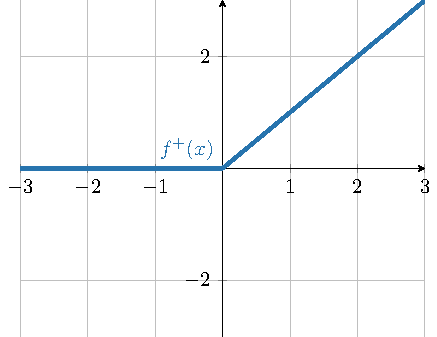
\includegraphics[scale=.8]{chapters/4-IntegrationRn/figures/figures-fplus.pdf}
      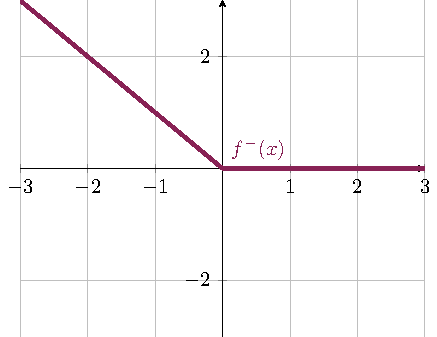
\includegraphics[scale=.8]{chapters/4-IntegrationRn/figures/figures-fminus.pdf}
\end{center}
    \end{example}
    
    \begin{proposition}
    $f(\bm{x}) = f^+(\bm{x}) - f^-(\bm{x})$.
    \end{proposition}


    \begin{proposition}
    Suppose that $f(\bm{x})$ is integrable on $\R^n$, and $g(\bm{y})$ is integrable on $\R^m$.  Then $h(\bm{x},\bm{y}) = f(\bm{x})g(\bm{y})$ is integrable on $\R^{n+m}$, and 
    $$\int_{\R^{n+m}} h \ dV \ dW = \int_{\R^n} f \ dV \int_{\R^n} g \ dW$$
    \end{proposition}
    
    \begin{remark}
        \textbf{Warning:} Note that $\bm{x}$ and $\bm{y}$ are necessarily different variables.  Furthermore, $$\int_{\R^{n}} f(\bm{x})g(\bm{x}) \ dV \neq \int_{\R^n} f(\bm{x}) \ dV \int_{\R^n} g(\bm{x}) \ dV$$
    \end{remark}

    \begin{example}
        Consider the functions $f(x) = x^2$, $g(x) = x$, and the region $A = [0,1] \subset \R$.  Observe that $$\int_0^1 f(x)g(x) \ dx = \int_0^1 x^3 \ dx \neq \left(\int_0^1 x^2 \ dx\right)\left(\int_0^1 x \ dx\right)$$
        The correct interpretation of the right hand side should be 
        $$\int_{A \times A} x^2y \ dA$$
        We will see how to calculate this in the next section.
    \end{example}
    
\subsection{Exercises}

\begin{problem}{examplesboundedboundedsupport}
Come up with examples of
       \begin{enumerate}
           \item a multivariable function that is not bounded.
           \item a multivariable function that does not have bounded support.
           \item A multivariable function that is neither bounded nor has bounded support.
       \end{enumerate}
\end{problem}

\begin{problem}{supportnoninterval}
    Come up with an example of a function $f(x) : \R \to \R$ with bounded support, but $\textnormal{supp}(f)$ is not an interval $[a.b]$.
\end{problem}

\begin{problem}{boundedboundedsupportvspace}
    Prove that if $f$ and $g$ are functions that are bounded with bounded support, then $f+g$ and $\lambda f$ are also functions that are bounded with bounded support.
\end{problem}

\begin{problem}{cube1}
    Explicitly describe and sketch the dyadic cube $C_{\langle1,1\rangle,2}$ in $\R^2$.
\end{problem}

\begin{problem}{cube2}
    Explicitly describe and sketch the dyadic cube $C_{\langle1,1,1\rangle,1}$ in $\R^3$.
\end{problem}

\begin{problem}{estimate}
    Consider the subset $C_{\langle1,1\rangle,2}$ in $\R^2$, and let $f(x,y) = x^2 + y^2$.  Calculate $M_{C_{\langle1,1\rangle,2}}(f)$ and $m_{C_{\langle1,1\rangle,2}}(f)$.
\end{problem}

\begin{problem}{estimate2}

Consider the subset $C_{\langle1,1\rangle,2}$ in $\R^2$, and let $f(x,y) = \frac{1}{x^2 + y^2}$.  Calculate $M_{C_{\langle1,1\rangle,2}}(f)$ and $m_{C_{\langle1,1\rangle,2}}(f)$.
    
\end{problem}


\begin{problem}{sup1}
     Consider the subset $C_{0,2}$ in $\R^1$, and let $f(x) = x^2$.  Calculate $M_{C_{0,2}}(f)$ and $m_{C_{0,2}}(f)$.
\end{problem}

\begin{problem}{sup2}
     Consider the subset $C_{0,2}$ in $\R^1$, and let $f(x) = \frac{1}{x}$.  Calculate $M_{C_{0,2}}(f)$ and $m_{C_{0,2}}(f)$.
\end{problem}

\begin{problem}{supnoinequality}
    Show that if $f(x) < g(x)$ for all $x$, then it is not necessarily the case that $\sup(f(x)) < \sup(g(x))$ for all $x$. (\textbf{Hint}: consider the function $f(x) := \left\{
		\begin{array}{ll}
			x & \text{ if } 0 \leq x < 1 \\
			0 & \text{ otherwise}
		\end{array}
		\right.$)
\end{problem}

\begin{problem}{supinfsum}
    Let $A, B \subset \R$ be nonempty sets.  Define the subset $A+ B$ by 
    $$A + B := \{ z \in \R \ | \ \text{there exist } x\in X, y \in Y \text{ such that } z = x+y\}$$

    \begin{subproblems}
        \item Show that $\sup(A+B) = \sup(A) + \sup(B)$.
        \item Show that $\inf(A+B) = \inf(A) + \inf(B)$.
    \end{subproblems}

\end{problem}

\begin{problem}{supinfdiff}
    Let $A, B \subset \R$ be nonempty sets.  Define the subset $A- B$ by 
    $$A + B := \{ z \in \R \ | \ \text{there exist } x\in X, y \in Y \text{ such that } z = x-y\}$$


    \begin{subproblems}
        \item Show that $\sup(A-B) = \sup(A) - \inf(B)$.
        \item Show that $\inf(A-B) = \inf(A) - \sup(B)$.
    \end{subproblems}

    
\end{problem}


\begin{problem}{supincomplete}

    Consider the set $A = \{x \in \Q \ | \ x^2 < 2 \}$.  
    
    \begin{subproblems}
        \item Do $\text{max}(A)$ or $\text{min}(A)$ exist?
        \item Find $\sup(A)$ and $\inf(A)$.  
    \end{subproblems}
    
    
    
\end{problem}

\begin{problem}{supinfexample}

    Consider the set $A = \{ \frac{n}{n+1} \ | \ n \in \N \}$.  

    
    \begin{subproblems}
        \item Do $\text{max}(A)$ or $\text{min}(A)$ exist?
        \item Find $\sup(A)$ and $\inf(A)$.  
    \end{subproblems}
\end{problem}


\begin{problem}{boundsdarboux}
    Prove that $U_N(f) \geq L_N(f)$.
\end{problem}

\begin{problem}{upperdarbouxexist}
    Let $f: \R^n \to \R$ be a continuous function that is bounded with bounded support. Prove that $U(f) := \lim_{N \to \infty} U_N(f)$ exists.  (You will need to use exercise \ref{problem:boundedincreasing}).
    
    \fixthis{reference problem}
\end{problem}

\begin{problem}{lowerdarbouxexist}
    Let $f: \R^n \to \R$ be a continuous function that is bounded with bounded support. Prove that $L(f) := \lim_{N \to \infty} L_N(f)$ exists. (You will need to use exercise \ref{problem:boundeddecreasing}).
\end{problem}

\begin{problem}{riemannintegrabletodarboux}
    Let $\bm{R_{k,N}} \in C_{\bm{k},N}$ be an arbitrary sampling of the dyadic partition, and define 
    $$R_N(f) := \sum_{C \in D_N(\R^n)} f(\bm{R_{k,N}}) \textnormal{vol(C)}$$
    
    Prove that if $f$ is integrable, then
    $$\lim_{N\to\infty} R_N(f) = \int_{\R^n}f \ dV $$

    (\textbf{Hint:} use the squeeze theorem!)
\end{problem}


\begin{problem}{strictineq}
    Give an example of an integrable function $f$ such that $$\left|\int_{\R^n} f \ dV\right| < \int_{\R^n} |f| \ dV$$
    (that is, an example of strict inequality)
\end{problem}

\begin{problem}{supfg}
    Let $f,g : \R^n \to \R$ be integrable functions, and consider the function $\sup(f,g)$ defined by $$\sup(f,g)(\bm{x}) := \sup(f(\bm{x}),g(\bm{x}))$$ Show that $\sup(f,g)$ is integrable.
    (\textbf{Hint:} Write $\sup(f,g)$ in terms of $f^+,f^-,g^+,g^-$).
\end{problem}

\begin{problem}{inffg}
    Let $f,g : \R^n \to \R$ be integrable functions, and consider the function $\inf(f,g)$ defined by $$\inf(f,g)(\bm{x}) := \inf(f(\bm{x}),g(\bm{x}))$$ Show that $\inf(f,g)$ is integrable.
    (\textbf{Hint:} Write $\inf(f,g)$ in terms of $f^+,f^-,g^+,g^-$).
\end{problem}



\section{Calculating multivariable integrals}

    \begin{motivating}
        Given a region $B \subset \R^n$ and an integrable function $f$, how can we compute $\int_B f(\bm{x}) \ dV$?
    \end{motivating}

    \begin{theorem}[Fubini]
    Let $f(\bm{x}): \R^n \to \R$ be a continuous function that is bounded with bounded support, and let $(i_1, \cdots i_n)$ be a permutation of the set $\{1, \cdots, n\}$. Then 
    
    $$\int_{\R^n} f(\bm{x}) \ dV = \int_{-\infty}^{\infty} \left( \cdots \left(\int_{-\infty}^{\infty} f(\bm{x}) \ dx_{i_1} \right) \cdots \right) \ dx_{i_n}$$

    \end{theorem}

    That is, we can compute an integral $\int_{\R^n} f(\bm{x}) \ dV$ as an iterated integral, in any variable order!

    \begin{example}
        Let $R$ be the region $[0,1] \times [0,1]$.  Compute the integral 
        $$\iint_R xe^{xy} \ dA $$
        By Fubini's theorem, there are two iterated integrals we can use (namely, $\int_0^1\int_0^1 xe^{xy} \ dx \ dy$ or $\int_0^1\int_0^1 xe^{xy} \ dy \ dx$).  

        However, observe that the former requires integration by parts.  However, we can compute 
        \begin{align*}
            \iint_R xe^{xy} \ dA  &= \int_0^1\int_0^1 xe^{xy} \ dy \ dx \\
            &= \int_0^1 [e^{xy}] \bigg|_{y=0}^{y=1} \ dx \\
            &= \int_0^1 e^{x}-1 \ dx \\
            &= e-2
        \end{align*}
        
    \end{example}


    \begin{remark}
        \fixthis{Relationship to Clairaut's theorem} (see corollary \ref{clairautcorollary}).
    \end{remark}

    Typically, the most difficult thing to do in multivariable integration is to visualize the region that you're integrating over.  

    \begin{example}
        Compute the volume of the solid region enclosed between the graph of  $f(x,y) = y$ and the $xy$-plane, over the region below:

        \begin{example}
    \begin{center}
            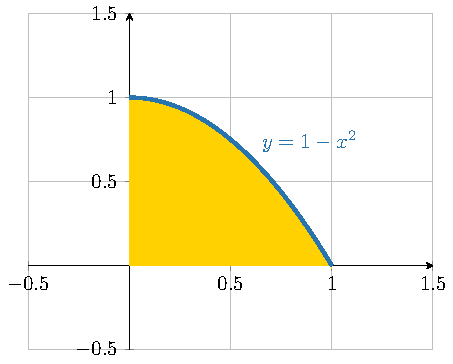
\includegraphics[scale=.7]{chapters/4-IntegrationRn/figures/figures-1-xsquaredregion.pdf}
    \end{center}
        \end{example}
        
    \end{example}

    \begin{example}
    Calculate the integral of $f(x,y,z) = xyz$ over the region $W$ in the first octant (that is, $x, y, z \geq 0$) bounded by $z = 4 - y^2$, $z = 0$, $y = 2x$, and $x= 0$.

    We can sketch this region as the region between $z=0$ and the parabolic cylinder ($z = 4 - y^2$), sitting above the triangle cut out by $x=0$, $y = 2x$, and $y=2$. We can thus write the region $W$ as 
    $$\{(x,y,z) \ | \ 0 \leq z \leq 4-y^2, 0 \leq x \leq \frac{y}{2}, 0 \leq y \leq 2\}$$
    Thus, we can compute the integral as $$\int_0^2\int_0^\frac{y}{2}\int_0^{4-y^2} xyz \ dz \ dx \ dy = \frac{2}{3}$$

    Alternatively, we can sketch this region as the region between $x=0$ and the plane $x = \frac{y}{2}$, sitting above the parabola cut out by $z = 4 - y^2$, $z=0$, and $y=0$.  We can thus write the region $W$ as 
    $$\{(x,y,z) \ | \ 0 \leq x \leq \frac{y}{2}, 0 \leq z \leq 4-y^2, 0 \leq y \leq 2\}$$
    Thus, we can also compute the integral as $$\int_0^2\int_0^{4-y^2}\int_0^\frac{y}{2} xyz \ dx \ dz \ dy = \frac{2}{3}$$

    As Clairaut's theorem stipulates, we can choose the iterated integral in the order that we want.
    \end{example}

    \begin{example}
        Compute the integral of $f(x,y) = \frac{1}{\ln(x)}$ over the domain $D$ bounded by $x = e^y$ and $x= e^{\sqrt{y}}$.

    \begin{center}
        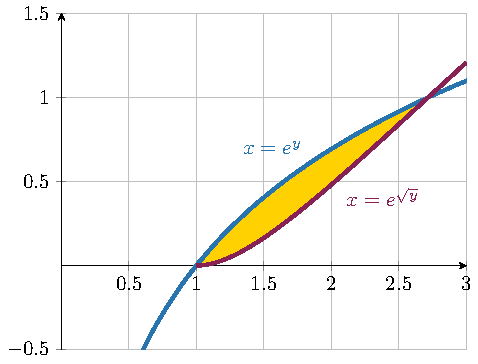
\includegraphics{chapters/4-IntegrationRn/figures/figures-intersectfubini.pdf}
    \end{center}
        
    \end{example}

\begin{theorem}[Decomposition of Domains]
        Let $K$ be a compact (closed and bounded) subset in $\R^n$ such that its boundary $\partial D$ has volume zero.  Furthermore, let $K = K_1 \cup K_2$, such that $K_1$ and $K_2$ are compact, and the intersection $K_1 \cap K_2$ has volume 0\footnote{Typically, $K_1 \cap K_2$ will be an ($n-1$)-dimensional subset (like the graph of a function $f : \R^{n-1} \to \R$, as in theorem \ref{thm:graphvolume0})}. 
    
    
    Let $f : K \to \R$ be a continuous function.  Then $f$ is integrable over $K_1$ and $K_2$, and 
    $$\int_K f(\bm{x}) \ dA = \int_{K_1} f(\bm{x}) \ dA + \int_{K_2} f(\bm{x}) \ dA $$ 
    \end{theorem}

\begin{example}
    Evaluate the double integral of $f(x,y) = 1-2x$ over the region $K$ as drawn below:

    \begin{center}
        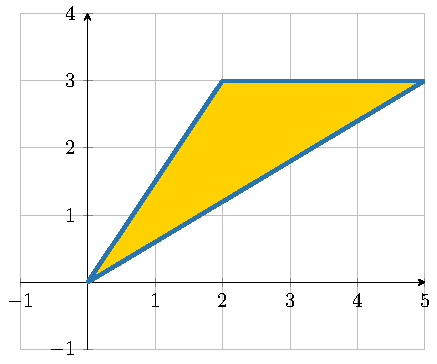
\includegraphics{chapters/4-IntegrationRn/figures/figures-decomposek.pdf}
    \end{center}

    We can decompose $K$ into two regions, $K_1$ and $K_2$ defined as $$K_1 = \{(x,y) \ | \ 0 \leq x \leq 2, \frac{3}{5}x \leq y \leq \frac{3}{2}x\}$$ and 
    $$K_2 = \{(x,y) \ | \ 2 \leq x \leq 5, \frac{3}{5}x \leq y \leq 3 \}$$  
    Note that $K_1$ and $K_2$ are both \textbf{vertically simple} (which simplifies calculating the integral). 

    \begin{center}
        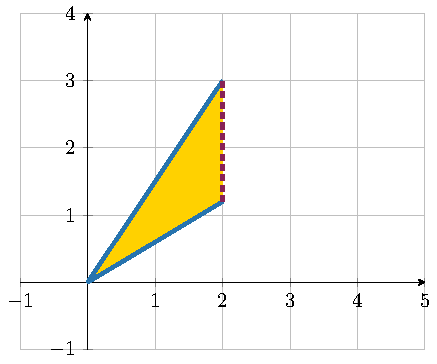
\includegraphics{chapters/4-IntegrationRn/figures/figures-decomposek1.pdf}
        The region $K_1$
        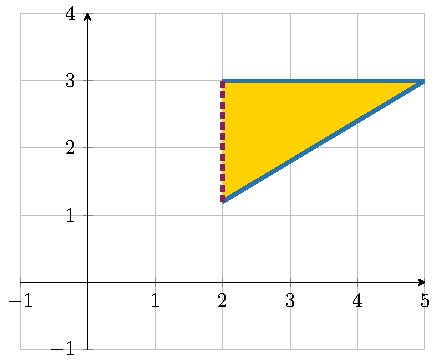
\includegraphics{chapters/4-IntegrationRn/figures/figures-decomposek2.pdf}
        The region $K_2$
    \end{center}

    Observe that $K = K_1 \cup K_2$, and the intersection $K_1 \cap K_2$ is the curve $\{(x,y) \ | \ \frac{6}{5} \leq y \leq 3, x=2 \}$, which has volume 0.
    Therefore, 
    \begin{align*}
        \iint_K 1-2x \ dA &= \iint_{K_1} 1-2x \ dA + \iint_{K_2} 1-2x \ dA\\
        &= \int_0^2\int_{\frac{3}{5}x}^{\frac{3}{2}x} 1-2x \ dy \ dx + \int_2^5\int_{\frac{3}{5}x}^{3} 1-2x \ dy \ dx \\
        &= \int_0^2 (1-2x)(\frac{3}{2}x-\frac{3}{5}x) \ dx + \int_2^5 (1-2x)(3-\frac{3}{5}x) \ dx \\
        &= -3 + -13.5 = -16.5        
    \end{align*}
    
    
    
\end{example}




\begin{definition}
    A subset $D \subset \R^2$ is \textbf{vertically simple}\define{vertically simple} if it is the region between graphs of two continuous functions $y = g_1(x)$ and $y = g_2(x)$ over a fixed interval of $x$-values $[a,b]$.
\end{definition}

\begin{example}
   The regions $K_1 = \{(x,y) \ | \ 0 \leq x \leq 2, \frac{3}{5}x \leq y \leq \frac{3}{2}x\}$ and $K_2 = \{(x,y) \ | \ 2 \leq x \leq 5, \frac{3}{5}x \leq y \leq 3 \}$ are both \textbf{vertically simple}. 
\end{example}

\begin{definition}
    A subset $D \subset \R^2$ is \textbf{horizontally simple}\define{horizontally simple} if it is the region between graphs of two continuous functions $x = h_1(y)$ and $x = h_2(y)$  over a fixed interval of $y$-values $[c,d]$.
\end{definition}

\begin{example}
    The region $K = \{(x,y) \ | \ \frac{2}{3}y \leq x \leq \frac{5}{3}y, 0 \leq y \leq 3\}$ is horizontally simple.  \textbf{Warning:} Be careful about the inequalities!

    We could therefore have instead computed 
    \begin{align*}
        \iint_K 1-2x \ dA &= \int_0^3\int_{\frac{2}{3}y}^{\frac{5}{3}y} 1-2x \ dx \ dy \\
        &= \int_0^3 [x-x^2] \bigg|_{\frac{2}{3}y}^{\frac{5}{3}y} \ dy\\
        &= \int_0^3 \frac{5}{3}y - (\frac{5}{3}y)^2 - \frac{2}{3}y + (\frac{2}{3}y)^2 \ dx \\
        &= -16.5        
    \end{align*}
\end{example}

\subsection{Exercises}

\begin{problem}{int1}
    Let $R$ be the region $[1,2] \times [2,4]$.  Compute the integral 
        $$\iint_R e^{3x-y} \ dA = \int_1^2\int_2^4 e^{3x-y} \ dy \ dx$$
\end{problem}

\begin{problem}{fub1}
    Let $R$ be the region $[0,1] \times [0,1]$.  Compute the integral 
        $$\iint_R xe^{xy} \ dA $$
\end{problem}

\begin{problem}{int3}
    Compute the integral $\iint_R x^2\tan(y) \ dA$ for $R$ the rectangle $[0,2] \times [0, \frac{\pi}{3}]$
\end{problem}

\begin{problem}{int4}
    Compute the integral $\iint_R \frac{x}{1+xy} \ dA$ for $R$ the rectangle $[0,1] \times [0, 1]$
\end{problem}

\begin{problem}{int5}
    Find the volume of the solid region enclosed between the graph of  $f(x,y) = \frac{1}{\sqrt{x+y}}$ and the $xy$-plane, over the rectangle $[0,4] \times [0,5]$.	
\end{problem}

\begin{problem}{fub2}
    Compute the integral of $f(x,y) = \frac{1}{\ln(x)}$ over the domain $D$ bounded by $x = e^{4y}$ and $x= e^{2\sqrt{y}}$.
\end{problem}

\begin{problem}{int6}
    Find the volume of the region bounded by $y = 1-x^2$, $z = 1$, $y = 0$, and $z+y=2$.
\end{problem}

\begin{problem}{symmetry}
    The volume contained in a sphere of radius 2 in $\R^3$ is $\frac{32\pi}{3}$.  What is the value of the following integral?  $$\int_{-2}^0\int^{0}_{-\sqrt{4-x^2}}\int_{0}^{\sqrt{4-x^2-y^2}} 1 \ dz \ dy \ dx$$
    
\end{problem}

\begin{problem}{3dint1}
    Integrate $f(x,y,z) = x$ over the region $W$ bounded above by $z = 4-x^2-y^2$ and below by $z=x^2+3y^2$ in the octant $x \geq 0$, $y \geq 0$, $z \geq 0$.
\end{problem}

\begin{problem}{3dint2}
    Find the volume between the intersection of the surfaces $z = x^2 + y^2$ and $z = 10 - x^2 - y^2$.
\end{problem}

\begin{problem}{3dint3}
    Compute $\iiint_W x \ dV$, where $W$ is the region in the first octant below the planes $z = 1-x$ and $z = 3 - x- y$.
\end{problem}










\section{Integrability}\label{sec:integrability}

In the previous sections, we have defined the notion of integrability, which we will restate below:

\begin{definition}
    Let $f: \R^n \to \R$ be a bounded function with bounded support.
    We say that $f$ is \textbf{integrable} if $U(f) = L(f)$.
    
    The \textbf{integral} of $f$ is $$\int_{\R^n} f(\bm{x}) \ dV := U(f) = L(f)$$
    \end{definition}

\begin{proposition}
    Let $f: \R^n \to \R$ be a bounded function with bounded support.  Then the following are equivalent:

    \begin{enumerate}
        \item $f$ is integrable.
        \item For any $\varepsilon > 0$, there exists $N$ such that for all $n > N$, $$U_n(f) - L_n(f) < \varepsilon$$
        \item For any $\varepsilon > 0$, there exists $N$ such that, $$U_N(f) - L_N(f) < \varepsilon$$
    \end{enumerate}
    
\end{proposition}

    \begin{proof}
        To see that (1) is equivalent to (2), we expand out the definitions.  That is, $f$ is integrable if and only if $$\lim_{N \to \infty} \left(U_N(f) - L_N(f)\right) = 0$$  
        However, this is equivalent to (2) by proposition \ref{epsilonenough} and exercise \ref{problem:boundsdarboux} (which tells us that $U_N(f) - L_N(f) \geq 0$).

        To see that (2) is equivalent to (3), observe from proposition \ref{darbouxmonotone} that $U_N(f) - L_N(f) \leq U_{N+1}(f) - L_{N+1}(f)$
    \end{proof}



The examples we've had so far are the following:
        
    \begin{theorem}
     If $f : \R^n \to \R$ is a continuous function that is bounded with bounded support, then $f$ is integrable.   
    \end{theorem}


    \begin{definition}
    Let $f: \R^n \to \R$ be a function, and let $A \subset \R^n$.  The \textbf{oscillation}\define{oscillation} of $f$ over $A$ is defined as $$\text{osc}_A(f) := M_A(f) - m_A(f)$$
    \end{definition}

    \begin{center}
        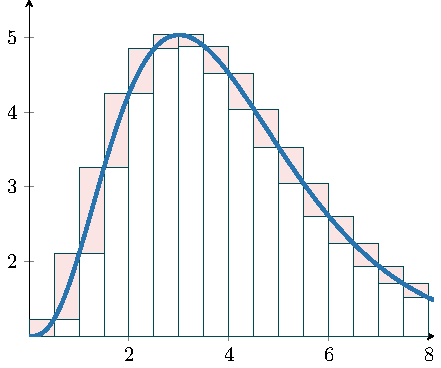
\includegraphics{chapters/4-IntegrationRn/figures/figures-integraloscillation.pdf}
    \end{center}
    
    \begin{theorem}
    A function $f: \R^n \to \R$ is integrable if and only if
    \begin{enumerate}
        \item $f$ is bounded with bounded support
        \item For all $\varepsilon > 0$, there exists $N$ such that $$\sum_{\{C \in D_N \ | \ \text{osc}_C(f) > \varepsilon \}} \textnormal{vol}_n C < \varepsilon$$
    \end{enumerate}
    \end{theorem}

\begin{proof}
    fixthis
\end{proof}

\begin{proposition}
        If $f: \R^n \to \R$ has bounded support, then there are finitely many cubes $C_{\bm{k},N}$ where $\textnormal{osc}_{C_{\bm{k},N}}(f) \neq 0$.
    \end{proposition}

\begin{example}
    \begin{theorem}
        If $f: \R^n \to \R$ is a continuous function that is bounded with bounded support, then $f$ is integrable.
    \end{theorem}

\begin{proof}
    Let $\varepsilon > 0$.  For a fixed vector $\bm{k}$, we can always find $M_{\bm{k}}$ such that for $m > M_{\bm{k}}$, 
    $$\textnormal{osc}_{C_{\bm{k},m}}(f) < \varepsilon$$
    since $f$ is continuous.

    There are finitely many cubes to consider, so we can take $M = \textnormal{max}\{M_{\bm{k}}\}$. So

    $$\sum_{C \in D_M(\R^n)} \textnormal{osc}_C(f) \textnormal{vol}(C) < \sum_{C \in D_M(\R^n)} \varepsilon \frac{1}{2^{Mn}}$$
\end{proof}

    That is, there are \textbf{no cubes} where $\textnormal{osc}_C(f) > \varepsilon$.
\end{example}

\begin{example}

    \begin{proposition}
        The function: $g(x) := \left\{
		\begin{array}{ll}
			1 & \text{ if } x \in [0,1] \text{ and }  x \notin \Q \\
			0 & \text{ otherwise}
		\end{array}
		\right.$ is \textbf{not} integrable.
    \end{proposition}

    \begin{proof}
    For all $m$, $\textnormal{osc}_{C_{\bm{k,m}}}(g) = 1$ for \textbf{every cube} contained in the region $[0,1]$.  Thus, $$\sum_{C \subset [0,1]} \textnormal{osc}_C(g) \textnormal{vol(C)} = \sum_{C \subset [0,1]} \textnormal{vol(C)} = 1$$
    
    But $$\sum_{C \subset [0,1]} \textnormal{osc}_C(g) \textnormal{vol(C)} < \sum_{C \in D_m(\R)} \textnormal{osc}_C(g) \textnormal{vol(C)}$$
    So $f$ is \textbf{not integrable}.        
    \end{proof}

\end{example}

From these examples, it is tempting to conclude if you cannot bound the oscillation of a function $f$, then $f$ is not integrable. However, this is not the case (see theorem \ref{IntegrabilityI}).

\begin{example}

    \begin{proposition}
      Consider the function: $$h(x) := \left\{
		\begin{array}{ll}
			\sin(\frac{1}{x}) & \text{ if } x \neq 0 \\
			0 & \text{ otherwise}
		\end{array}
		\right.$$

    \begin{center}
        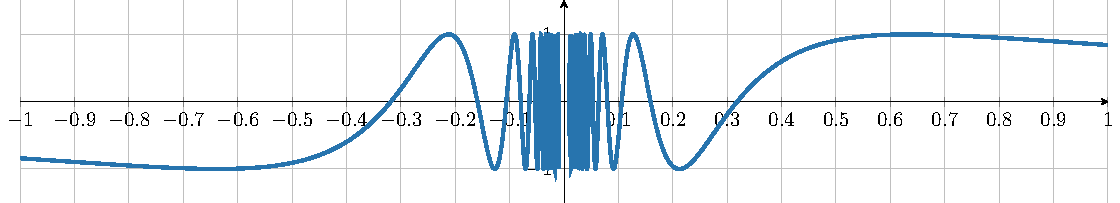
\includegraphics[scale=.7]{chapters/4-IntegrationRn/figures/figures-sin1x.pdf}
    \end{center}

    Observe that as $x$ approaches 0, $h(x)$ oscillates between $-1$ and $1$.  However, $h(x)$ \textbf{IS} integrable on any interval $[a,b] \subset \R^n$.  
    \end{proposition}
    
    \begin{proof}
     Observe that $h(x) := \left\{
		\begin{array}{ll}
			\sin(\frac{1}{x}) & \text{ if } x \neq 0 \\
			0 & \text{ otherwise}
		\end{array}
		\right.$  
is continuous everywhere except at $x=0$.  

    \begin{center}
        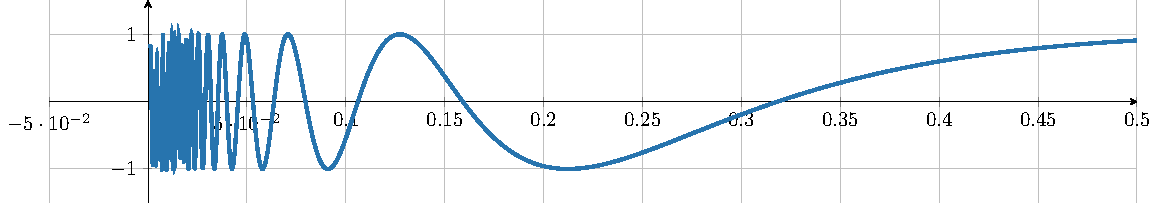
\includegraphics[scale=.7]{chapters/4-IntegrationRn/figures/figures-sin1xzoom.pdf}
    \end{center}

    Thus, if $D = C_{0,N}$ or $D=C_{-1,N}$, then $\textnormal{osc}_D(f) = 2$.

    However, for all other $C_{k,N}$, we can choose $M$ large enough so that $\textnormal{osc}_C(f) < \varepsilon$ for all $C$.  So
    \begin{align*}
    \sum_{C \in D_M(\R^n)} \textnormal{osc}_C(f) \textnormal{vol}(C) &= 4\textnormal{vol}(C) + \sum_{\substack{C \in D_M(\R^n) \\ C \neq D}} \textnormal{osc}_C(f) \textnormal{vol}(C)\\
    &= \frac{4}{2^{Mn}} + \sum_{\substack{C \in D_M(\R^n) \\ C \neq D}} \varepsilon \frac{1}{2^{Mn}}
    \end{align*}

    \end{proof}

\end{example}

The correct statement is as follows: a bounded function with bounded support $f: \R^n \to \R$ is integrable if you can bound the volumes of the cubes where $f$ oscillates too much.

\begin{theorem}[Integrability Criterion I]\label{IntegrabilityI}
    A function $f: \R^n \to \R$ is integrable if and only if
    \begin{enumerate}
        \item $f$ is bounded with bounded support
        \item For all $\varepsilon > 0$, there exists $N$ such that $$\sum_{\{C \in D_N(\R^n) \ | \ \text{osc}_C(f) > \varepsilon \}} \textnormal{vol}_n C < \varepsilon$$
    \end{enumerate}
    \end{theorem}

This is a useful theorem to have, but it is difficult to use in practice.  Here is another integrability theorem:

\begin{theorem}[Integrability Criterion II]\label{IntegrabilityII}
    Let $f: \R^n \to \R$ be a bounded function with bounded support.  If $f$ is continuous except on a set of volume zero, then $f$ is integrable.  
\end{theorem}

\begin{remark}
This is \textbf{not} an if and only if statement! We will see an example of a function that is integrable, but is discontinuous on a set whose volume is not defined\footnote{see example \ref{Thomae}}.

We will refine this integrability theorem to an if and only if statement in theorem \ref{integrabilityIII}
\end{remark}

\begin{proposition}
    A bounded set $X \subset \R^n$ has $n$-dimensional volume 0 if and only if for every $\varepsilon > 0$, there exists $M$ such that
    $$\sum_{\substack{C \in D_M(\R^n) \\ C \cap X \neq \varnothing}} \textnormal{vol}_n(C) < \varepsilon$$
\end{proposition}

\begin{example}
If $X \subset \R^n$ is a closed and bounded (compact) region, and $f : X \to \R$ is a continuous function, then $$\textnormal{vol}_{n+1}(\Gamma_f) = 0$$ \fixthis{ref}
\end{example}

\begin{example}
    The unit circle in $\R^2$, $S := \{(x,y) \ | \ x^2 + y^2 = 1\}$ has 2-dimensional volume 0.
\end{example}

\begin{example}
        Let $D$ be the unit disk in $\R^2$.  That is, $D := \{(x,y) \ | \ x^2 + y^2 \leq 1\}$.

        Then the indicator function $1_D(\bm{x}) : \R^2 \to \R$ is integrable by theorem \ref{IntegrabilityII}, as it not continuous on a subset of 2-dimensional volume 0.
    \end{example}

\begin{corollary}
        Let $f: \R^n \to \R$ be integrable, and let $g : \R^n \to \R$ be a bounded function.  If $f=g$ except on a set of volume 0, then $g$ is integrable, and
        $$\int_{\R^n} f \ dV = \int_{\R^n} g \ dV$$
\end{corollary}


Let us now turn to some pathological functions:

We first describe a set that does not have $n$-dimensional volume.

\begin{example}\label{nonintegable}
    Consider the set $A \subset \R$ defined by 
    $$A := \{ x \in \R \ | \ x \in (0,1) \text{ and }  x \in \Q \}$$
    $A$ does not have volume, since the indicator function $1_A(x) : \R \to \R$ is not integrable \fixthis{example}
    
    ($\text{osc}(1_A) = 1$ on the interval $(0,1)$)
 
\end{example}


    \begin{example}\label{Thomae}
    Consider Thomae's function, which is defined as the function $$g(x) := \left\{
		\begin{array}{ll}
			\frac{1}{q} & \text{ if } x \in (0,1) \text{ and }  x =\frac{p}{q} \text{ is rational, written in lowest terms, with } p \in \Z, q \in \N \\
			0 & \text{ otherwise}
		\end{array}
		\right.$$


\begin{center}
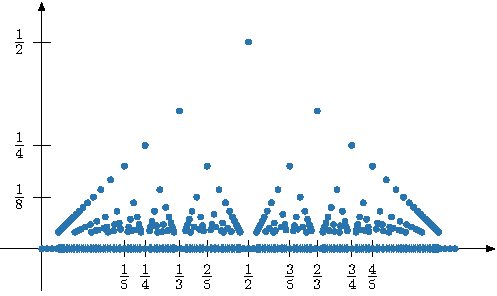
\includegraphics{chapters/4-IntegrationRn/figures/figures-thomaesfunction.pdf}
\end{center}
  

    We see that $f$ is discontinuous precisely on the set $A := \{ x \in \R \ | \ x \in (0,1) \text{ and }  x \in \Q \}$

    However, by theorem \ref{IntegrabilityI}, we see that we can bound the volumes of the cubes where $f$ oscillates too much, and hence Thomae's function is integrable.
    
    \end{example}

So let us now turn to generalzing theorem \ref{IntegrabilityII}.

\begin{definition}
        An open ball $B \subset \R^n$ of radius $\delta > 0$, centered on $\bm{x}$, is the set
        $$B = \left\{ \bm{v} \in \R^n \ | \ ||\bm{x} - \bm{v}|| < \delta \right\}$$
    \end{definition}

\begin{definition}
        A set $X \subset \R^n$ has \textbf{measure zero}\define{meaure zero} if for every $\varepsilon > 0$, there exists an infinite sequence of open balls $B_i$ such that 
    $$X \subset \bigcup B_i \qquad \textnormal{and} \qquad \sum \text{vol}_n(B_i) < \varepsilon$$
    \end{definition}

\begin{proposition}
    A set of volume $0$ has measure zero.
    \end{proposition}

    \begin{remark}
    On the other hand, it is possible that $X$ has measure zero, but $\text{vol}(X)$ is undefined.
    \end{remark}

\begin{example}
        The set $$A = \Q \cap [0,1]$$ that is, the set of rational numbers in the interval $[0,1]$, has undefined volume\footnote{see example \ref{nonintegable}}.  However, the set $$A = \Q \cap [0,1]$$ has measure zero!

        We can enumerate the elements of $A$ as $$\{F_n\} := \{0,1, \frac{1}{2}, \frac{1}{3}, \frac{2}{3}, \frac{1}{4}, \frac{2}{4}, \frac{3}{4}, \frac{1}{5} \cdots \}$$

        To each element in the sequence, we can associate $B_n$ as the open ball of radius $\frac{1}{2^{n+1}}$, centered at $F_n$.

        We can then see that $$A \subset \bigcup B_n \qquad \textnormal{and} \qquad \sum \text{vol}_n(B_n) < \varepsilon$$
    \end{example}

\begin{theorem}[Integrability Criterion III]\label{integrabilityIII}
    A function $f: \R^n \to \R$ is integrable if and only if
    \begin{enumerate}
        \item $f$ is bounded with bounded support
        \item $f$ is continuous except on a set of measure 0.
    \end{enumerate}
    \end{theorem}

    \begin{example}
        Thomae's function is bounded with bounded support, and is continuous except on a set of measure 0.
    \end{example}
    











\subsection{Exercises}

\begin{problem}{integrabilitycounterexamples1}
Come up with (and prove) an example of a multivariable function that is not integrable.
\end{problem}

\begin{problem}{integrabilitycounterexamples2}
Come up with (and prove) an example of a function where $|f|$ is integrable, but $f$ is not integrable.
\end{problem}

\section{Change of variables}

\begin{motivating}
    Consider the unit ball (that is, the solid region bounded by the unit sphere) in $\R^3$, denoted
    $$B := \{(x,y,z) \ | x^2 + y^2 + z^2 \leq 1\}$$
    
    Observe that it is difficult to compute $\int_B 1 \ dV$ as an iterated integral.  
\end{motivating}

In this section, we will see that changing coordinate systems will make integration easier.

\subsection{Polar coordinates}

Recall that we've studied vectors in $\R^2$ primarily in terms of their components.  However, we have seen that it is equivalent to describe a position vector in terms of its magnitude and direction.  Polar coordinates is a way to describe vectors in $\R^2$ using this perspective:

\begin{definition}
Given a point $(x,y)$ in rectangular coordinates, we can convert it to a point $(r,\theta)$ in polar coordinates by setting 
    $$r = \sqrt{x^2 + y^2} \qquad \textnormal{and} \qquad \tan(\theta) = \frac{y}{x} \ (\textnormal{assuming} \ x \neq 0)$$
\end{definition}

We can also convert from polar coordinates back to the standard rectangular coordinates:     
\begin{definition}
Given a point $(r,\theta)$ in polar coordinates, we can convert it to a point $(x,y)$ in rectangular coordinates by setting 
    $$x = r\cos(\theta) \qquad \textnormal{and} \qquad y = r\sin(\theta)$$
\end{definition}

    \begin{center}
        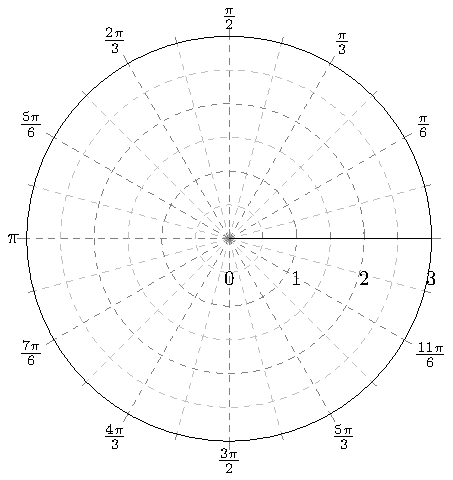
\includegraphics{chapters/4-IntegrationRn/figures/figures-polaraxes.pdf}
    \end{center}

\begin{example}
    The line $y=mx$ corresponds to the polar equation $$\theta = \tan^{-1}(m)$$  \fixthis{explain more}
\end{example}

\begin{example}
    The disk of radius $R$, centered at the origin, can be described in polar coordinates as the set of points $$\{(r,\theta) \ | \ r \leq R\}$$
\end{example}

Moreover, polar coordinates allows us to describe certain curves in $\R^2$ much more easily than in rectangular coordinates, such as the three-petaled rose described by $r = \cos(3\theta)$.

% \begin{center}
%     \begin{tikzpicture}[scale=.7]
%   \begin{polaraxis}[  xtick distance = deg(pi/4),
%   xtick = {0,0,deg((pi)/4),deg((pi)/2),deg((3*pi)/4),deg(pi),deg((5*pi)/4), deg((3*pi)/2), deg((7*pi)/4)},
%   xticklabels={,0,$\frac{\pi}{4}$,$\frac{\pi}{2}$,$\frac{3\pi}{4}$,$\pi$,$\frac{5\pi}{4}$, $\frac{3\pi}{2}$, $\frac{7\pi}{4}$,}
%  ]
% \addplot+ [
% color=UCLAdark,
% mark=none,
% domain=0:360,
% samples=600,
% ]
% {cos(3*x)};
% % equivalent to (x,{sin(..)cos(..)}), i.e.
% % the expression is the RADIUS
%   \end{polaraxis}

%   \end{tikzpicture}
%   \begin{tikzpicture}[scale=.65, >=latex]

% % Draw the lines at multiples of pi/12
% \foreach \ang in {0,...,31} {
%   \draw [lightgray] (0,0) -- (\ang * 180 / 16:4);
% }

% % Concentric circles and radius labels
% \foreach \s in {0, 1, 2, 3} {
%   \draw [lightgray] (0,0) circle (\s + 0.5);
%   \draw (0,0) circle (\s);
%   \node [fill=white] at (\s, 0) [below] {\scriptsize $\s$};
% }

% % Add the labels at multiples of pi/4
% \foreach \ang/\lab/\dir in {
%   0/0/right,
%   1/{\pi/4}/{above right},
%   2/{\pi/2}/above,
%   3/{3\pi/4}/{above left},
%   4/{\pi}/left,
%   5/{5\pi/4}/{below left},
%   7/{7\pi/4}/{below right},
%   6/{3\pi/2}/below} {
%   \draw (0,0) -- (\ang * 180 / 4:4.1);
%   \node [fill=white] at (\ang * 180 / 4:4.2) [\dir] {\scriptsize $\lab$};
% }

% % The double-lined circle around the whole diagram

% \fill [fill=red!50!black, opacity=0.5] plot [domain=0:2*pi]
%   (xy polar cs:angle=\x r, radius= {1});
% \draw [thick, color=red, domain=0:2*pi, samples=200, smooth]
%   plot (xy polar cs:angle=\x r, radius={1});
% \node [fill=white] at (2,1) {$r\leq 1$};

% \end{tikzpicture} 
% \end{center}

Polar coordinates are convenient when the domain of integration $R$ is an angular sector, or a \textbf{polar rectangle}.  That is, if we can describe $R$ in the form: 
    $$R = \{ (r, \theta) \ | \ {\theta_1} \leq \theta \leq {\theta_2}, r_1 \leq r \leq r_2\}$$
    

    
\begin{center}
        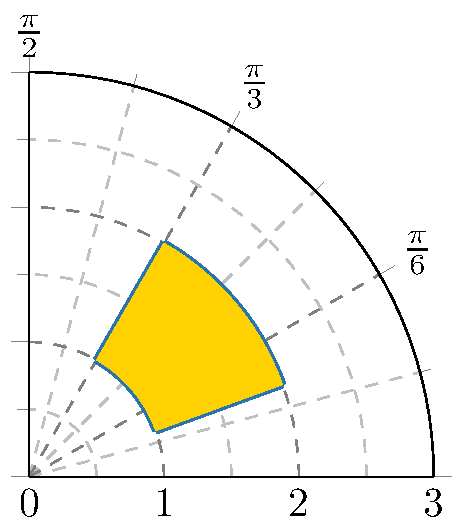
\includegraphics{chapters/4-IntegrationRn/figures/figures-polarrectangle.pdf}
    \end{center}

\begin{definition}
A region $R$ is called \textbf{radially simple} if it is the region between graphs of two continuous functions $r_1(\theta)$ and $r_2(\theta)$ over a fixed interval of $\theta$-values.  That is, 
$$R = \{ (r, \theta) \ | \ \alpha \leq \theta \leq \beta, r_1(\theta) \leq r \leq r_2(\theta)\}$$
\end{definition}

\begin{example}
\begin{center}
        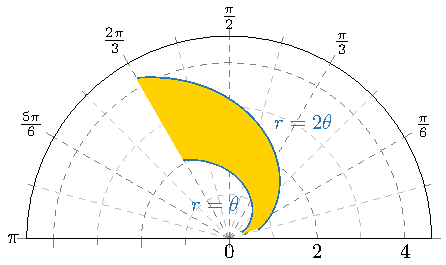
\includegraphics{chapters/4-IntegrationRn/figures/figures-radiallysimple.pdf}
\end{center}
\end{example}

\begin{theorem}[Double integral in polar coordinates]
If $f(x,y)$ is a continuous function on a radially simple domain $R$, then $$\iint_R f(x,y) \ dA = \int_\alpha^\beta \int_{r= r_1(\theta)}^{r= r_2(\theta)} f(r\cos(\theta), r\sin(\theta)) \ r \ dr \ d\theta$$
\end{theorem}

\begin{remark}
    Observe that there is an extra $r$ term in the integral - we will see why when we consider the general change of variables formula.
\end{remark}

\begin{example}
    Find the area of the region enclosed by the cardioid $r = 2 - 2\sin(\theta)$.

\begin{center}
        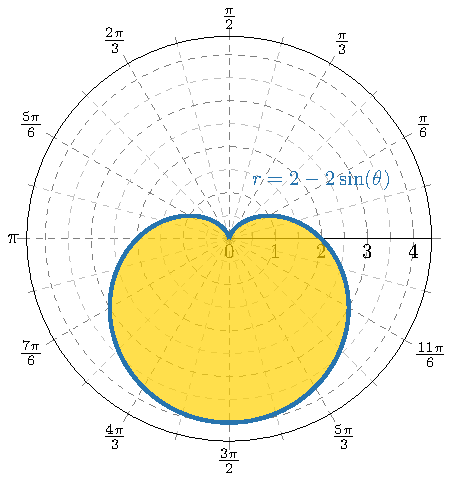
\includegraphics{chapters/4-IntegrationRn/figures/figures-cardioid.pdf}
    \end{center}
\end{example}

\subsection{Cylindrical coordinates}

We can extend polar coordinates in $\R^2$ to cylindrical coordinates in $\R^3$ in the following way:

\begin{definition}
Given a point $(x,y,z)$ in Euclidean coordinates, we can convert it to a point $(r,\theta,z)$ in cylindrical coordinates by setting 
    $$z = z \qquad \textnormal{and} \qquad r = \sqrt{x^2 + y^2} \qquad \textnormal{and} \qquad \tan(\theta) = \frac{y}{x} \ (\textnormal{assuming} \ x \neq 0)$$
\end{definition}

We can also convert from cylindrical coordinates back to the standard Euclidean coordinates:     
\begin{definition}
Given a point $(r,\theta,z)$ in polar coordinates, we can convert it to a point $(x,y,z)$ in rectangular coordinates by setting 
    $$x = r\cos(\theta) \qquad \textnormal{and} \qquad y = r\sin(\theta)\qquad \textnormal{and} \qquad z=z$$
\end{definition}

\begin{example}
    Let $B$ denote the unit ball (that is, the solid region bounded by the unit sphere) in $\R^3$.  Write $\int_B 1 \ dV$ as an iterated integral in cylindrical coordinates.
\end{example}

\subsection{Spherical coordinates}

Another coordinate system for $\R^3$ can be defined in terms of spherical coordinates:

    \begin{center}
        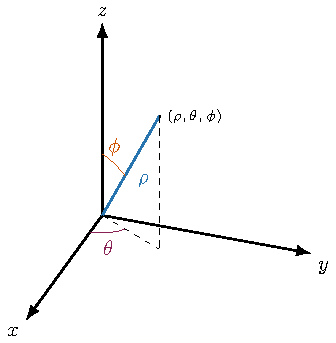
\includegraphics{chapters/4-IntegrationRn/figures/figures-spherical.pdf}
    \end{center}
    
\begin{proposition}
    Given a point $(\rho,\theta,\phi)$ in spherical coordinates, we can convert it to the standard Euclidean coordinates by setting 
    $$x = \rho\sin(\phi)\cos(\theta) \qquad y = \rho\sin(\phi)\sin(\theta) \qquad z=\rho\cos(\phi)$$
    \end{proposition}
    
    \begin{proposition}
    Given a point $(x,y,z)$ in standard Euclidean coordinates, we can convert it to spherical coordinates by setting 
    $$\rho = \sqrt{x^2 + y^2 +z^2} \qquad \tan(\theta) = \frac{y}{x} \qquad \cos(\phi) = \frac{z}{\rho}$$
    \end{proposition}

\begin{definition}
A solid region $R \subset \R^3$ is called \textbf{centrally simple} if $R$ is of the form
$$R = \{ (\rho, \theta, \phi) \ | \ \theta_1 \leq \theta \leq \theta_2, \phi_1 \leq \phi \leq \phi_2, \rho_1(\theta,\phi) \leq \rho \leq \rho_2(\theta,\phi)\}$$
\end{definition}

\begin{example}
    PICTURE
\end{example}

\begin{theorem}[Triple integrals in spherical coordinates]
Let $f(x,y,z)$ be a continuous function on a centrally simple region $R$. Write $$f(\rho\sin(\phi)\cos(\theta),\rho\sin(\phi)\sin(\theta),\rho\cos(\phi)) = g(\theta, \phi, \rho)$$  Then $\iiint_R f(x,y,z) \ dV$ equals
$$\int_{\theta_1}^{\theta_2} \int_{\phi_1}^{\phi_2}\int_{\rho = \rho_1(\theta,\phi)}^{\rho = \rho_2(\theta,\phi)} g(\theta, \phi, \rho) \ \rho^2 \sin(\phi) \ d\rho \ d\phi \ d\theta$$
\end{theorem}

\begin{remark}
    Observe that there is an extra $\rho^2 \sin(\phi)$ term in the integral - we will see why when we consider the general change of variables formula.
\end{remark}

\begin{example}
    Let $B$ denote the unit ball (that is, the solid region bounded by the unit sphere) in $\R^3$.  Write $\int_B 1 \ dV$ as an iterated integral in spherical coordinates. 
\end{example}




\subsection{General Change of Variables}

\begin{motivating}
    Why do we need to add extra terms when changing coordinates?
\end{motivating}

\subsubsection{Linear change of variables}

We will first study what happens for linear change of variable maps:

\fixthis{references}

\begin{proposition}
     A function $T : \R^n \to \R^m$ is a \textbf{linear map} if  for all $\bm{u}, \bm{v} \in \R^n$ and for all $\lambda \in \R$,
     
     \begin{itemize}
        \item $T(\bm{u} + \bm{v}) = T(\bm{u}) + T(\bm{v})$.
        \item $T(\lambda \bm{u}) = \lambda T(\bm{u}))$.
    \end{itemize}
    \end{proposition}

\begin{theorem}
    A map $T: \R^n \to \R^m$ is linear if and only if there is a matrix $A \in M_{m \times n}(\R)$ such that $$T(\bm{x}) = A\bm{x}$$  
    We call $A$ the \textbf{standard matrix} of $T$.
    \end{theorem}
    
\begin{definition}
    The \textbf{standard matrix} $A$ of a linear map $T: \R^n \to \R^m$ is given by
    \begin{equation*}
A = 
\begin{bmatrix}
\vert & \vert & & \vert \\
    T(\bm{e_1})   & T(\bm{e_2}) & \cdots & T(\bm{e_n})  \\
    \vert & \vert & & \vert
\end{bmatrix} \in M_{m \times n}(\R)
\end{equation*}
\end{definition}

% \begin{center}\begin{tikzpicture}[scale=.65]

% \begin{scope}
% \clip (-3,-3) rectangle (3,3);
 
% %grid
% \draw[step=0.5cm, gray!20!white, very thin] (-3,-3) grid (3,3);
% \draw[step=1cm, gray!60!white, thin] (-3,-3) grid (3,3);
% % Axes
%     \draw [latex-latex] (-3,0) -- (3,0) node [below left] {$x$};
%     \draw [latex-latex] (0,-3) -- (0,3) node [below right] {$y$};
% \draw[color=UCLAdark, line width=1.10pt, -Latex] (0, 0) -- (1,0);
% \draw[color=red!80!black, line width=1.10pt, -Latex] (0, 0) -- (0,1);

% \end{scope}

% \begin{scope}[xshift=9cm]
% %all you need to change are the entries in the matrix using the following 4 macros
% \pgfmathsetmacro{\entrya}{2}
% \pgfmathsetmacro{\entryb}{1}
% \pgfmathsetmacro{\entryc}{1}
% \pgfmathsetmacro{\entryd}{1.5}


% \clip (-3,-3) rectangle (3,3);
% %grid
% \draw[step=0.5cm, gray!20!white, very thin] (-3,-3) grid (3,3);
% \draw[step=1cm, gray!60!white, thin] (-3,-3) grid (3,3);
% % Axes
%     \draw [latex-latex] (-3,0) -- (3,0) node [below left] {$x$};
%     \draw [latex-latex] (0,-3) -- (0,3) node [below right] {$y$};
% \foreach \x in {-5,...,5} {
% \draw[domain=-3:3,smooth,variable=\t,color=UCLAblue!60!white, thick]plot (\entrya*\t+\x*\entryb,\entryc*\t+\x*\entryd);
% }

% \foreach \y in {-5,...,5} {
% \draw[domain=-3:3,smooth,variable=\t,color=mered!60!white, thick]plot (\entryb*\t+\y*\entrya,\entryd*\t+\y*\entryc);
% }


% \draw[color=UCLAdark, line width=1.10pt, -Latex] (0, 0) -- (\entrya, \entryc);
% \draw[color=red!80!black, line width=1.10pt, -Latex] (0, 0) -- (\entryb, \entryd);
% \end{scope}



% \draw[thick,-latex] (4,0) to[out=60,in=120] node[midway,font=\scriptsize,above] {$T_B$} (5,0);

% \end{tikzpicture}
%     \end{center}


\begin{example}
    Consider the linear map $T(x,y) = (Ax + By, Cx + Dy)$.  What is the image of the unit square $R = [0,1] \times [0,1]$ under $G$?
    \end{example}

\begin{proposition}
    Let $P$ be the parallelogram spanned by $\bm{u} = \langle A, B \rangle$ and $\bm{v} = \langle C, D \rangle$ in $\R^2$.
    \begin{equation*}
        \Big|\textnormal{det}\begin{bmatrix}
A & B \\
C & D
\end{bmatrix}\Big| = \textnormal{area}(P)
    \end{equation*}
    
       That is, the absolute value of a $2 \times 2$
determinant equals the area of the parallelograms spanned by the rows.
    \end{proposition}


\begin{theorem}[Expansion along the $i$-th row]
    Let $A$ be an $n \times n$ matrix, and let $A_{ij}$ denote the $(n-1) \times (n-1)$ matrix obtained by deleting row $i$ and column $j$ from $A$.
    $$\textnormal{det}(A) = (-1)^{i+1}a_{i,1}\textnormal{det}(A_{i1}) + \cdots +  (-1)^{i+n}a_{i,n}\textnormal{det}(A_{in})$$
    
    \end{theorem}
    
    \begin{example}
    The \textbf{determinant} of a $3 \times 3$ matrix is denoted and defined as follows:
\begin{equation*}
\textnormal{det} 
\begin{bmatrix}
a_1 & b_1 & c_1 \\
a_2 & b_2 & c_2 \\
a_3 & b_3 & c_3 \\
\end{bmatrix} = a_1\begin{vmatrix}
b_2 & c_2 \\
b_3 & c_3
\end{vmatrix} - b_1\begin{vmatrix}
a_2 &  c_2 \\
a_3 &  c_3
\end{vmatrix} + c_1\begin{vmatrix}
a_2 & b_2 \\
a_3 & b_3 \\
\end{vmatrix}
\end{equation*}

    \end{example}


\begin{theorem}
    Let $D$ be the parallelpiped spanned by $\bm{u}$, $\bm{v}$, and $\bm{w}$ in $\R^3$.  Then
    \begin{equation*}
\textnormal{volume}(D) = |\bm{u} \cdot (\bm{v \times w})| = | \textnormal{det}
\begin{bmatrix}
\bm{u} \\
\bm{v} \\
\bm{w} \\
\end{bmatrix}|
\end{equation*}

    
    \end{theorem}

\begin{theorem}
    Let $D$ be the parallelpiped spanned by $\bm{v_1}, \bm{v_2}, \cdots \bm{v_n}$ in $\R^n$.  Then
    \begin{equation*}
\textnormal{vol}_n(D) = | \textnormal{det}
\begin{bmatrix}
\bm{v_1} \\
\vdots \\
\bm{v_n} \\
\end{bmatrix}|
\end{equation*}

    
    \end{theorem}

\begin{corollary}
Let $T(\bm{x}) = A\bm{x}$ be a linear transformation from $\R^n \to \R^n$.  Then the volume of the image of the unit cube in $\R^n$ is $|\textnormal{det}A|$.


\end{corollary}
    
    \begin{theorem}
    The $n$-dimensional volume of a region $D \subset \R^n$ under a linear transformation $T(\bm{x}) = A\bm{x}$ is given by 
    $$\textnormal{vol}_n(T(D)) = |\textnormal{det}A|\textnormal{vol}_n(D)$$
    \end{theorem}



\subsubsection{Nonlinear change of variables}

\begin{motivating}
     What happens if $G : \R^n \to \R^n$ is a \textbf{non-linear} change of coordinates map?
\end{motivating}

If $G$ is differentiable, we can approximate $G$ with its \textbf{derivative} (aka its linear approximation).

\begin{definition}
    Let $f : A \subset \R^m \to \R^n$ be a multivariable function defined by $f_i  : A \subset \R^m \to \R$:
    \begin{equation*}
        f(\bm{x}) = \begin{bmatrix}
f^1(\bm{x}) \\
\vdots \\
f^n(\bm{x})
\end{bmatrix}
    \end{equation*}
    
    The \textbf{Jacobian matrix} of $f$ at $\bm{x_0}$ is 
    
    \begin{equation*}
        [J_f(\bm{x_0})] = \begin{bmatrix}
D_1f^1(\bm{x_0}) & D_2f^1(\bm{x_0}) & \cdots & D_mf^1(\bm{x_0}) \\
D_1f^2(\bm{x_0}) & D_2f^2(\bm{x_0}) & \cdots & D_mf^2(\bm{x_0}) \\
\vdots & \vdots & \vdots & \vdots\\
D_1f^n(\bm{x_0}) & D_2f^n(\bm{x_0}) & \cdots & D_mf^n\bm{x_0}) 
\end{bmatrix}
    \end{equation*}
    
    if the partial derivatives exist.
    
    \end{definition}

    \begin{theorem}[The derivative in coordinates]
    Let  $f : A \subset \R^m \to \R^n$ be a multivariable function.  If $f$ is \textbf{differentiable at} $\bm{x_0}$, then all the partial derivatives $D_if^j\bm{x_0})$ exist, and the standard matrix of $Df(\bm{x_0})$ is $[J_f(\bm{x_0})]$.  That is,
    $$Df(\bm{x_0})(\bm{h}) = [J_f(\bm{x_0})]\bm{h}$$
    
    \end{theorem}
    
    
    
    \begin{remark}
    The derivative of a function $f : \R^m \to \R^n$ at a point $x_0$ is the \textbf{approximation} of $f$ by a \textbf{linear transformation} at $x_0$.
    \end{remark}


    \begin{example}
    Given a differentiable map $G(u,v) = \left(x(u,v), y(u,v)\right)$, we can define its \textbf{Jacobian matrix}, $[J_G]$, as the matrix of partial derivatives:
    
    \begin{equation*}
        [J_G] = \begin{bmatrix}
\frac{\partial x}{\partial u} & \frac{\partial x}{\partial v} \\[1em]
\frac{\partial y}{\partial u} & \frac{\partial y}{\partial v}
\end{bmatrix}
    \end{equation*}
    
    The determinant of the Jacobian matrix is denoted $\textnormal{Jac}(G)$.
    $$\det([J_G]) = \textnormal{Jac}(G) = \frac{\partial x}{\partial u} \frac{\partial y}{\partial v} - \frac{\partial x}{\partial v}\frac{\partial y}{\partial u}$$
       
    \end{example}


\begin{proposition}
    Let $D \subset \R^n$ be a region such that $\textnormal{vol}_n(D)$ is small, and let $p \in D$.  Let $G: \R^n \to \R^n$ be differentiable map. Then

    $$\textnormal{vol}_n(G(D)) \approx |\det([J_G](\bm{p}))|\textnormal{vol}_n(D)$$

    That is, the the $n$-dimensional volume of $G(D)$ can be approximated by the $n$-dimensional volume of $[J_G](\bm{p})(D)$.
    \end{proposition}

\begin{motivating}
    When is $\textnormal{vol}_n(G(D)) = \textnormal{vol}_n(D)$?
\end{motivating}

There are a few problems that can occur:

    \begin{enumerate}
        \item $G$ might not be differentiable
        \item $\det([J_G](\bm{p})) = 0$.  That is, $J_G$ is not invertible.
        \item $G : \R^n \to \R^n$ is \textbf{not injective} on $D$.  That is, there exist points $\bm{x} \neq \bm{y} \in 
        D$ such that $G(\bm{x}) = G(\bm{y})$
    \end{enumerate}


\begin{example}
    Consider the linear map $T: \R^2 \to \R^2$ defined by $$T(x,y) = (x+y, 2x+2y)$$

    Note that $\textnormal{det} 
\begin{bmatrix}
1 & 1 \\
2 & 2 \\
\end{bmatrix} = 0$.

    
    
%         \begin{center}\begin{tikzpicture}[scale=.65]

% \begin{scope}
% \clip (-3,-3) rectangle (3,3);
 
% %grid
% \draw[step=0.5cm, gray!20!white, very thin] (-3,-3) grid (3,3);
% \draw[step=1cm, gray!60!white, thin] (-3,-3) grid (3,3);
% % Axes
%     \draw [latex-latex] (-3,0) -- (3,0) node [below left] {$x$};
%     \draw [latex-latex] (0,-3) -- (0,3) node [below right] {$y$};
% \draw[color=UCLAdark, line width=1.10pt, -Latex] (0, 0) -- (1,0);
% \draw[color=red!80!black, line width=1.10pt, -Latex] (0, 0) -- (0,1);

% \end{scope}

% \begin{scope}[xshift=9cm]
% %all you need to change are the entries in the matrix using the following 4 macros
% \pgfmathsetmacro{\entrya}{1}
% \pgfmathsetmacro{\entryb}{1}
% \pgfmathsetmacro{\entryc}{2}
% \pgfmathsetmacro{\entryd}{2}


% \clip (-3,-3) rectangle (3,3);
% %grid
% \draw[step=0.5cm, gray!20!white, very thin] (-3,-3) grid (3,3);
% \draw[step=1cm, gray!60!white, thin] (-3,-3) grid (3,3);
% % Axes
%     \draw [latex-latex] (-3,0) -- (3,0) node [below left] {$x$};
%     \draw [latex-latex] (0,-3) -- (0,3) node [below right] {$y$};
% \foreach \x in {-5,...,5} {
% \draw[domain=-3:3,smooth,variable=\t,color=UCLAblue!60!white, thick]plot (\entrya*\t+\x*\entryb,\entryc*\t+\x*\entryd);
% }

% \foreach \y in {-5,...,5} {
% \draw[domain=-3:3,smooth,variable=\t,color=mered!60!white, thick]plot (\entryb*\t+\y*\entrya,\entryd*\t+\y*\entryc);
% }


% \draw[color=UCLAdark, line width=1.10pt, -Latex] (0, 0) -- (\entrya, \entryc);
% \draw[color=red!80!black, line width=1.10pt, -Latex] (0, 0) -- (\entryb, \entryd);
% \end{scope}



% \draw[thick,-latex] (4,0) to[out=60,in=120] node[midway,font=\scriptsize,above] {$T$} (5,0);

% \end{tikzpicture}
%     \end{center}

\end{example}



\begin{example}
     Consider the polar coordinates map defined by $$G(r,\theta) = (r\cos(\theta), r\sin(\theta))$$

    $G$ is \textbf{not injective} on the region 
    $$R = \{ (r, \theta) \ | \ 0 \leq \theta \leq 3\pi, 0 \leq r \leq 2\}$$

    \fixthis{PICTURE}

    \end{example}

    \begin{example}
     Consider the polar coordinates map defined by $$G(r,\theta) = (r\cos(\theta), r\sin(\theta))$$

    $G$ \textbf{IS injective} on the region 
    $$R = \{ (r, \theta) \ | \ 0 < \theta < 2\pi, 0 < r < 2\}$$

    \end{example}


\begin{theorem}[Change of variables for volume]
    Let $K \subset \R^n$ be a compact set such that $\text{vol}_n(\partial K) = 0$.  Let $U \subset \R^n$ be an open set containing $K$. Let $$G : U \to \R^n$$ be a map such that 
    \begin{enumerate}
        \item $G$ is differentiable.
        \item $G$ is injective on the interior of $K$.  
        \item $\det [J_G] \neq 0$ on the interior of $K$.  
    \end{enumerate}
    Then
    $$\int_{G(K)} 1 \  dV = \int_K |\det [J_G]| \ dV$$
    \end{theorem}

\begin{theorem}[Change of variables]
    Let $K \subset \R^n$ be a compact set such that $\text{vol}_n(\partial K) = 0$.  Let $U \subset \R^n$ be an open set containing $K$. Let $$G : U \to \R^n$$ be a map such that 
    \begin{enumerate}
        \item $G$ is differentiable.
        \item $G$ is injective on the interior of $K$.  
        \item $\det [J_G] \neq 0$ on the interior of $K$.  
    \end{enumerate}
   
    Then if $f: G(K) \to \R$ is a continuous function, then 
    $$\int_{G(K)} f \  dV = \int_K (f \circ G) \ |\det [J_G]| \ dV$$
    \end{theorem}

    \begin{example}
    Consider the polar coordinates map defined by $$G(r,\theta) = (r\cos(\theta), r\sin(\theta))$$

    \begin{corollary}[Double integral in polar coordinates]
If $f(x,y)$ is a continuous function on a polar rectangle $G(R)$, then $$\iint_{G(R)} f(x,y) \ dA = \int_{\theta_1}^{\theta_2} \int_{r= r_1}^{r= r_2} f(r\cos(\theta), r\sin(\theta)) \ r \ dr \ d\theta$$
\end{corollary}
    \end{example}

    \begin{example}
        Let $D$ be the region in the first quadrant defined by $$D = \{ (x,y) \ | \ 1 \leq xy \leq 4, 1 \leq y/x \leq 4 \}$$
    Compute $\iint_D (x^2 + y^2) \ dx \ dy$.
    \end{example}

\begin{remark}
    Sometimes, it is easier to find a map going in the \textit{wrong direction}, $$F(x,y) = (u(x,y),v(x,y))$$
    Then $G = F^{-1}$.
    \end{remark}
    
    %     \begin{figure}
    %     \centering
    %     \includegraphics[scale=0.45]{pictures/map.png}
    % \end{figure}
    
    \begin{theorem}
    If $G = F^{-1}$, and $\det [J_F] \neq 0$, then $\det [J_G] = \frac{1}{\det [J_F]}$
    \end{theorem}





    \subsection{Exercises}

    \begin{problem}{polargraph1}
    Sketch a graph of and find the area enclosed by the polar equation $r = \sin(2\theta)$.
    \end{problem}

    \begin{problem}{polargraph2}
    Sketch a graph of and find the area enclosed by the polar equation $r = 4\cos(\theta)$.
    \end{problem}

    \begin{problem}{polargraph3}
    Sketch a graph of and find the area enclosed by the polar equation $r = 1+\sin(\theta)$.
    \end{problem}

    \begin{problem}{polargraph4}
    Sketch a graph of and find the area enclosed by the polar equation $r = 2\cos(\theta) -1$.
    \end{problem}

    \begin{problem}{spherical}
        The volume of a sphere of radius 2 is $\frac{32\pi}{3}$.  What is the value of the following integral?$$\int_{-\frac{\pi}{4}}^{\frac{\pi}{4}}\int_0^\pi\int_0^2 \rho^2 \sin(\phi) \ d\rho \ d\phi \ d\theta$$
    \end{problem}

    \begin{problem}{polar1}
    Compute the integral $$\int_0^3\int_0^{\sqrt{9-y^2}}\int_0^1 z\sqrt{x^2 + y^2} \ dz \ dx \ dy$$
\end{problem}

\begin{problem}{change1}
    Let $D$ be the region in the first quadrant defined by $$D = \{ (x,y) \ | \ 1 \leq xy \leq 4, 1 \leq y/x \leq 4 \}$$
    Compute $\iint_D (x^2 + y^2) \ dx \ dy$.
\end{problem}

\begin{problem}{change2}
 Consider the parallelogram $P$ with vertices $A = (0,0)$, $B = (3,1)$, $C = (2,3)$, $D = (5,4)$.  
    \begin{subproblems}
    \item Find a change of variables $G(u,v) = (x(u,v), y(u,v))$ that transforms the unit square to $P$.  Compute the determinant of the Jacobian of $G$.
    \item Use your work from the previous problem to compute the integral $$\iint_P e^{3x-y} \ dA$$.
    \end{subproblems}
    
\end{problem}

\begin{problem}{change3}
    Consider the change of variables $G(u,v) = (uv^{-1}, uv)$ that transforms the square $[1,2]\times[1,2]$ to the region $D$ in the first quadrant bounded by $1 \leq xy \leq 4$ and $1 \leq \frac{y}{x} \leq 4$. Use this to compute the integral $$\iint_D x^2+y^2 \ dA$$.
\end{problem}

\chapter{Integration on manifolds}

\section{Integrals on curves and surfaces}

\begin{motivating}
How do you calculate the length of this curve?
\end{motivating}

\fixthis{PICTURE}

\begin{motivating}
How do you calculate the surface area of a sphere?
\end{motivating}

\fixthis{PICTURE}

Observe that these sets have $3$-dim volume 0.  To calculate arclength or surface area, we will need to \fixthis{integrate over the appropriate region. }

\subsection{Integrals on curves}

\fixthis{recall}


\begin{definition}
    A \textbf{vector-valued function} is a function $\bm{r}(t): \R \to \R^n$, given by
    $$\bm{r}(t) = \langle x_1(t),x_2(t), \cdots x_n(t) \rangle$$
    
    where all of the $x_i(t) : \R \to \R$ are single-variable functions.
    
    $\bm{r}(t)$ is also called a \textbf{parametrization} (with \textbf{parameter} $t$).
    \end{definition}


    We should think of a vector-valued function $\bm{r}(t)$ as describing the motion of a particle in $\R^n$. 

    \begin{definition}
    The path traced out by a parametrization is called a \textbf{parametric curve}.
    \end{definition}

\begin{center}
        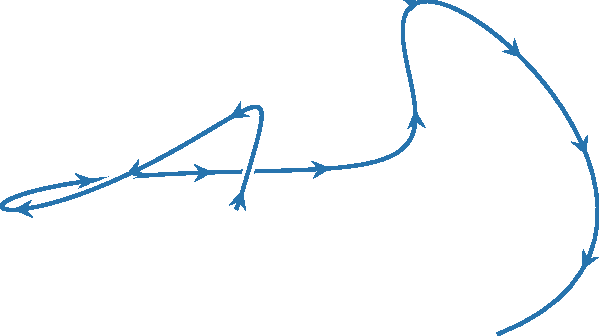
\includegraphics{chapters/5-IntegrationManifolds/figures/figures-paramcurve.pdf}
\end{center}

If a vector valued function $\bm{r}(t)$ describes the motion of an object in $\R^n$, how can we find the \textbf{distance} traveled by that object (from $t=a$ to $t=b$)?

\begin{definition}
    If $\bm{r}(t)$ models the motion of the object, the distance $D$ traveled (from $t=a$ to $t=b$) is given by the integral of the speed. That is, 
    $$D = \int_a^b ||\bm{r}'(t)|| \ dt$$ 
    \end{definition}

\begin{example}
Let $\bm{r}(t) = \langle \cos(t), \sin(t), 2 \rangle$ model the motion of a particle in $\R^3$. 
    
    Sketch the vector valued function, and find the distance traveled from $t=0$ to $t = 4\pi$.
\end{example}

How are your answers related to the parametric curve of $\bm{r}(t)$, and the length of the parametric curve?

\begin{definition}[]
    A \textbf{strict parametrization} of a curve $\mathcal{C} \subset \R^n$ is a vector-valued function $\bm{r}(t) : (a,b) \subset \R \to \mathcal{C}$ satisfying the following conditions:
    \begin{enumerate}    
        \item $\bm{r}(t)$ surjects onto $\mathcal{C}$.
        \item $\bm{r}(t)$ is injective for all $t \in (a,b)$.
        \item $\bm{r}(t)$ is differentiable.
        \item $\bm{r}'(t) \neq \bm{0}$ for all $t \in (a,b)$.    
    \end{enumerate}
    
    \end{definition}

     \begin{definition}[Arclength]
    Let $\mathcal{C}$ be a curve in $\R^n$, and let $\bm{r}(t) : (a,b) \to \R^n$ be a (strict) parametrization of $\mathcal{C}$.  
    
    Then the \textbf{arclength of $\mathcal{C}$} is defined to be the integral 
    
    $$\int_a^b ||\bm{r}'(t)|| \ dt$$
    
    \end{definition}

    \begin{example}
        Find the arc length of the vector-valued function $\bm{h}(t) = \langle -\sin(t), \cos(t), t \rangle$ from $t=0$ to $t=2\pi$.
    \end{example}

    \begin{definition}[Scalar line integral]
    Let $f : \R^n \to \R$ be a function of $n$ variables, and let $\mathcal{C}$ be a curve in $\R^n$.

    Let $\bm{r}(t) : (a,b) \to \R^n$ be a (strict) parametrization of $\mathcal{C}$.  Then the \textbf{scalar line integral  of $f$ over $\mathcal{C}$} is denoted $\int_\mathcal{C} f \ ds$, and is defined as the integral

    $$\int_\mathcal{C} f \ ds := \int_a^b f(\bm{r}(t)) \ ||\bm{r}'(t)|| \ dt$$
    
    \end{definition}

    \begin{center}
        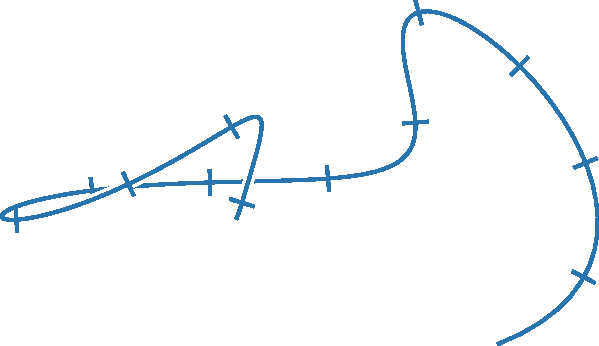
\includegraphics{chapters/5-IntegrationManifolds/figures/figures-partitioncurve.pdf}
    \end{center}

    \begin{example}
        Let $C$ be the helix, parametrized by $\bm{h}(t) = \langle -\sin(t), \cos(t), t \rangle$ for $0 \leq t \leq 3\pi$.  Calculate
    $$\int_C (x + y + z) \ ds$$
    \end{example}

    \begin{example}
     Find the total mass of a wire in the shape of a parabola $y = x^2$ for $1 \leq x \leq 4$ (in centimeters), with mass density given by $$\rho(x,y) = \frac{y}{x} \  \textnormal{grams/cm}$$   
    \end{example}

    \begin{motivating}
        Can you find a strict parametrization of the circle $x^2+y^2=1$ in $\R^2$?
    \end{motivating}

    Nope!

    \fixthis{recall}

    
    \begin{definition}
        Let $A \subset \R^n$.  We say that $A$ is an\textbf{ open subset of $\R^n$} if $A$ does not contain any of its boundary points.  That is, $$A \cap \partial A = \varnothing$$
    \end{definition}

     \begin{example}
        The interval $(a,b)$ is open in $\R$.  The sets $[a,b)$ and $[a,b]$ are \textbf{not open}.
    \end{example}

    \begin{example}
        The set $B_r(\bm{0}) := \{ \bm{v} \in \R^n \ | \ ||\bm{v}|| < 1\} $ is open in $\R^n$.  
    \end{example}

\begin{definition}[Parametrization]
    Let $\mathcal{C}$ be a curve in $\R^n$.  Let $A \subset \R$ be a subset such that $\textnormal{vol}_1(\partial A) = 0$.  Let $X \subset A$ be a subset such that $A - X$ is open.  Then  $\gamma : A \to \R^n$ is a \textbf{parametrization of} $\mathcal{C}$ if 
    
    \begin{enumerate}
        
        \item $\mathcal{C} \subset \gamma(A)$ (that is, $\gamma$ surjects onto $\mathcal{C}$).
        \item $\gamma(A - X) \subset \mathcal{C}$, and $\gamma : A - X \to \mathcal{C}$ is injective. 
        \item $\gamma(t)$ is differentiable for all $t \in A - X$.
        \item $\gamma'(t) \neq \bm{0}$ for all $t \in A - X$. 
        \item $\text{vol}_1(X) = 0$.
    \end{enumerate}
    
    \end{definition}

\begin{remark}
If $\gamma$ is a parametrization of $\mathcal{C}$, then $\gamma: (A-X) \to \mathcal{C} - \gamma(X)$ is a strict parametrization.
\end{remark}
    
\begin{example}
    Let $S^1$ be the circle $x^2+y^2=1$ in $\R^2$.
    
    Let $A = [0,2\pi] \subset \R$, and let $X = \{0, 2\pi\}$.  Then $A-X = (0,2\pi)$ is open, and $\text{vol}_1(X) = 0$.

    Let $\gamma(t) = \langle \cos(t) , \sin(t) \rangle$.


        \begin{enumerate}
        
        \item $S^1 = \gamma([0,2\pi])$.
        \item $\gamma(0,2\pi) \subset S^1$, and $\gamma : (0,2\pi) \to S^1$ is injective. 
        
        \item $\gamma'(t) = \langle -\sin(t), \cos(t) \rangle$.
        \item $\gamma'(t) \neq \bm{0}$ for all $t \in (0,2\pi)$.
    \end{enumerate}

    
    Therefore, $\gamma(t) = \langle \cos(t), \sin(t) \rangle$ parametrizes $S^1$:
    \end{example}

    \begin{definition}[Scalar line integral]
    Let $f : \R^n \to \R$ be a function of $n$ variables, and let $\mathcal{C}$ be a curve in $\R^n$.

    Let $\bm{r}(t) : (a,b) \to \R^n$ be a parametrization of $\mathcal{C}$.  Then the \textbf{scalar line integral  of $f$ over $\mathcal{C}$} is denoted $\int_\mathcal{C} f \ ds$, and is defined as the integral

    $$\int_\mathcal{C} f \ ds := \int_a^b f(\bm{r}(t)) \ ||\bm{r}'(t)|| \ dt$$
    \end{definition}


\subsection{Integrals on Surfaces in $\R^3$}

\begin{motivating}
    How do you calculate the surface area of a sphere?
\end{motivating}

\fixthis{picture}

\begin{definition}[]
    A \textbf{strict parametrization} of a surface $\mathcal{S} \subset \R^3$ is a multivariable function $G(u,v) : U \subset \R^2 \to \mathcal{S}$ satisfying the following conditions:
    \begin{enumerate}
        \item $U$ is an open set.
         
        \item $G(u,v)$ surjects onto $\mathcal{S}$.
        \item $G(u,v)$ is injective for all $\bm{u} \in U$.
     
        \item $G(u,v)$ is differentiable for all $\bm{u} \in U$ (that is, $\frac{\partial G}{\partial u}$ and $\frac{\partial G}{\partial v}$ exist).

        \item $[J_G(u,v)]$ is injective for all $\bm{u} \in U$.
    \end{enumerate}
    
    \end{definition}


\begin{theorem}
    The following statements are equivalent about a linear transformation $T : \R^n \to \R^m$ with standard matrix $A$:
    
    \begin{enumerate}
        \item $T$ is injective.
        \item The only solution to the equation $A\bm{x} = \bm{0}$ is $\bm{x} = \bm{0}$.
        \item If the equation $A\bm{x} = \bm{b}$ has a solution, it is unique.
        \item The columns of $A$ are linearly independent.
    \end{enumerate}
    
    \end{theorem}

\begin{example}
        Consider the surface $\mathcal{S}$ defined by $$\{(x,y,z) \ | \ x^2 + y^2 < 1, z=0\}$$ \fixthis{turn into polar rectangle}
        
        Let $U = \{(r,\theta) \ | \ 0 < r < 1, \ 0 < \theta < 2\pi\} \subset \R^2$, and let $$G(r,\theta) = \langle r\cos(\theta), r\sin(\theta), 0 \rangle$$

\begin{enumerate}               
        \item $G(u,v)$ surjects onto $\mathcal{S}$.
        \item $G(u,v)$ is injective for all $\bm{u} \in U$.
        
        \item $G(u,v)$ is differentiable for all $\bm{u} \in U$.

        \item $[J_G(u,v)]$ is injective for all $\bm{u} \in U$.
    \end{enumerate}

    So $G(r,\theta)$ is a strict parametrization of $\mathcal{S}$.
        
    \end{example}

    \begin{example}
        Consider the surface $\mathcal{S}$ defined by $$\{(x,y,z) \ | \ z= f(x,y), a < x < b, c < y < d\}$$

        Parametrize the surface $\mathcal{S}$.
    \end{example}


\begin{remark}
    Let $\mathcal{S}$ be a surface (strictly) parametrized by $G(u,v)$, and consider a point $P = G(u_0,v_0)$ on $S$.
    
    \vspace{1em}
    
    Observe that the functions $G(u,v_0)$ and $G(u_0,v)$ are curves on the surface $\mathcal{S}$ that intersect at $P$.
    \end{remark}
    
%    \begin{center}
%        \includegraphics[scale=0.4]{pictures/surfacetangent.png}
%    \end{center}

\begin{theorem}
    The tangent plane to $\mathcal{S}$ at a point $G(u_0,v_0)$ is spanned by the vectors $$\frac{\partial G}{\partial u}(u_0,v_0) = \left\langle \frac{\partial x}{\partial u}(u_0,v_0), \frac{\partial y}{\partial u}(u_0,v_0), \frac{\partial z}{\partial u}(u_0,v_0) \right\rangle$$
    $$\frac{\partial G}{\partial v}(u_0,v_0) = \left\langle \frac{\partial x}{\partial v}(u_0,v_0), \frac{\partial y}{\partial v}(u_0,v_0), \frac{\partial z}{\partial v}(u_0,v_0) \right\rangle$$
    \end{theorem}
    
    \begin{motivating}
        What is an equation for the tangent plane to $\mathcal{S}$ at a point $G(u_0,v_0)$?
    \end{motivating}
    
    \fixthis{recall}
\begin{theorem}
    Let $D$ be the parallelogram in $\R^3$ spanned by $\bm{u}$ and $\bm{v}$. Then
    $$\textnormal{area}(D) = ||\bm{u \times v}||$$
    \end{theorem}

\begin{theorem}
    Let $\mathcal{S}$ be a surface (strictly) parametrized by a function $\bm{\gamma} :  U \subset \R^{2} \to \R^3$.  Then the area of a parallelogram at a point $\gamma(\bm{u}) \in S$ is given by $$\textnormal{area}(D) = \left|\left|\frac{\partial \gamma}{\partial u}(\bm{u}) \times \frac{\partial \gamma}{\partial v}(\bm{u})\right|\right|$$ 
    \end{theorem}

\begin{definition}
    Let $\mathcal{S}$ be a surface (strictly) parametrized by a function $\bm{\gamma} :  U \subset \R^{2} \to \R^3$.  Then the \textbf{surface area of $\mathcal{S}$} is denoted by $\int_\mathcal{S} \ dA$, and defined to be
    $$\int_\mathcal{S} \ dS := \int_U \left|\left|\frac{\partial \gamma}{\partial u} \times \frac{\partial \gamma}{\partial v}\right|\right| \ dA$$
    \end{definition}

\begin{motivating}
    Can you find a strict parametrization of the sphere $x^2+y^2+z^2=1$ in $\R^3$?
\end{motivating}

\begin{definition}[Parametrization]
    Let $\mathcal{S} \subset \R^3$ be a surface.  Let $A \subset \R^2$ be a subset such that $\textnormal{vol}_2(\partial A) = 0$.  Let $X \subset A$ be a subset such that $A - X$ is open.  Then a map $\gamma : A \to \R^3$ parametrizes $\mathcal{S}$ if 
    
    \begin{enumerate}
        \item $\mathcal{S} \subset \gamma(A)$ (that is, $\gamma$ surjects onto $\mathcal{S}$).
        \item $\gamma(A - X) \subset \mathcal{S}$, and $\gamma : A - X \to \mathcal{S}$ is injective. 

        \item $\gamma$ is differentiable for all $\bm{u} \in A-X$   
        \item $[J_\gamma(\bm{u})]$ is injective for all $\bm{u} \in A - X$. 
        
        \item $\text{vol}_2(X) = 0$ and for any compact subset $C \subset \mathcal{S}$, $\text{vol}_2(\gamma(X) \cap C) = 0$.
    \end{enumerate}
    
    \end{definition}

\begin{definition}
    Let $X \subset \R^n$ be a bounded subset.  We say that $X$ has $k$\textbf{-dimensional volume 0} ($\textnormal{vol}_k(X) = 0$) if
    $$\lim_{N \to \infty} \sum_{\substack{C \in D_N(\R^n) \\ C \cap X \neq \varnothing}} \left(\frac{1}{2^N}\right)^k = 0$$
    
    \end{definition}
    

    
    \begin{definition}
    Let $X \subset \R^n$ be an arbitrary subset.  We say that $X$ has $k$\textbf{-dimensional volume 0} ($\textnormal{vol}_k(X) = 0$) if for all $R > 0$, $B_R(\bm{0}) \cap X$ has volume 0.
    
    \end{definition}

    \begin{example}
    Let $S^2$ be the sphere $x^2+y^2+z^2=1$ in $\R^3$.

\vspace{1em}

    Let $A = \{(\theta, \phi) \ | \ 0 \leq \theta \leq  2\pi, \ 0 \leq \phi \leq  \pi\} \subset \R^2$, and let $X = \partial A$.  Then $A-X$ is open, and $\text{vol}_2(X) = 0$.

    Let $\gamma(\theta, \phi) = \langle \cos(\theta)\sin(\phi), \sin(\theta)\sin(\phi), \cos(\phi) \rangle$.

    
        \begin{enumerate}
        
        \item $S^2 = \gamma(A)$.
        \item $\gamma(A-X) \subset S^2$, and $\gamma : (A-X) \to S^2$ is injective. 
        
        \item $[J_\gamma(\theta, \phi)] = 
\begin{bmatrix}
-\sin(\theta)\sin(\phi) & \cos(\theta)\cos(\phi) \\
\cos(\theta)\sin(\phi) & \sin(\theta)\cos(\phi) \\
0 & -\sin(\phi)
\end{bmatrix}$
    \end{enumerate}

    
    Therefore, $\gamma(\theta, \phi)$ parametrizes $S^2$.
    \end{example}

\begin{example}
    Calculate the surface area of sphere $S^2 \subset \R^3$.
\end{example}



\subsection{Exercises}

\begin{problem}{arclengthinR2}
    Let $f: \R \to \R$ be a differentiable function.  Find a formula for the arclength of the graph of $y = f(x)$ from $x=a$ to $x=b$.
\end{problem}

\begin{problem}{arclengthinpolar}
    Let $\langle r(t), \theta(t)\rangle$ be a parametrization of a curve in polar coordinates.  Find a formula for the arclength of the curve from $t=a$ to $t=b$.  (\textbf{Hint}: convert to rectangular coordinates).
\end{problem}

\begin{problem}{Bernoulli}
    The Bernoulli spiral has parametrization $\bm{r}(t) = \langle e^t\cos(4t), e^t\sin(4t) \rangle$.  Find the arclength of the Bernoulli spiral from the point $(1,0)$ to the point $(e^{\frac{\pi}{2}}, 0)$.
\end{problem}


\begin{problem}{helix1}
Let $C$ be the helix, parametrized by $\bm{r}(t) = \langle \cos(t), \sin(t), t \rangle$ for $0 \leq t \leq 3\pi$.  Calculate
    $$\int_C (x + y + z) \ ds$$
\end{problem}

\begin{problem}{line1}
Let $f(x,y,z) = ye^{z^2}$.  Compute $\int_C f \ ds$ for the piecewise linear path from $(0,0,1)$ to $(2,0,0)$ to $(1,1,1)$
\end{problem}

\begin{problem}{line2}
Let $C$ be the line segment from $(0,0,0)$ to $(6,2,2)$. Calculate $$\int_C x+yz \ ds$$
\end{problem}


\begin{problem}{paramcurve}
    Parametrize the curve $C$ in $\mathbb{R}^3$ formed by intersecting the cylinder $x^2 + y^2 = 1$ and the plane $x + y + z = 1$ in $\mathbb{R}^3$
\end{problem}

\begin{problem}{paramfunction}
    Find a parametrization of the graph of $f(x) = x^{\frac{1}{3}}$.
\end{problem}

\begin{problem}{paramreverse}
    Let $\bm{r}(t) : (a,b) \to \R^n$ be a parametrization of $\mathcal{C}$ from $\bm{r}(a) = P$ to $\bm{r}(b) = Q$.  Find a parametrization $\bm{s}(u)$ of $\mathcal{C}$ that starts at $Q$ and ends at $P$.

    \begin{subproblems}
    \item Can you use $\bm{s}(u)$ to calculate $\int_\mathcal{C} f \ ds$?
    \end{subproblems}
\end{problem}


\begin{problem}{param1}
 Find a compact region $D$ and a parametrization $\Phi : D \to \R^3$ that parametrizes the surface $S$ given as the set $\{(x,y,z) \ | \ z = x+y^2, \ 0 < x < y, \ 0 < y < 1 \}$.  Verify that $\Phi$ is a parametrization.
\end{problem}

\begin{problem}{surfaceint1}
    Let $S$ be the surface $\{(x,y,z) \ | \ z = x+y^2, \ 0 < x < y, \ 0 < y < 1 \}$.
    Compute the surface integral $\int_S (z-x) \ dA$.
\end{problem}

\begin{problem}{tangentplane}
    Let $S$ be a surface (strictly) parametrized by $G(u,v) = (u,v, f(u,v))$.  Find an equation for the tangent plane to $S$ at $P = G(u_0,v_0)$.
\end{problem}

\begin{problem}{surfaceareaplane}
    Find a parametrization of the plane $2x+y-z=2$, and find the area of the plane that lies below the triangle with vertices $(0,0,0)$, $(0,1,0)$, $(1,0,0)$.
    
\end{problem}

\begin{problem}{paramcone}
     Consider the cone defined by $M = \{(x,y,z) \ | \ x^2 + y^2 - z^2 = 0, \ 0 < z < 1\}$.  Find the regions $A$ and $X$ in $\R^2$ such that the map $\gamma(r,\theta) = \langle r\cos(\theta), r\sin(\theta), r$ is a parametrization of the cone.
\end{problem}

\begin{problem}{surfaceint2}
    Calculate the surface area of the cone defined by $M = \{(x,y,z) \ | \ x^2 + y^2 - z^2 = 0, \ 0 < z < 1\}$.
\end{problem}


\begin{problem}{paramsurface3}
     Show that $\gamma(u,v) = \langle u^2, uv, v^2 \rangle$ parametrizes the surface $M$ given by $xz-y^2 = 0$. 
\end{problem}

\begin{problem}
    Calculate $\int_S (z-x) \ dS$, where $S$ is the portion of the graph of $z = x + y^2$, where $0 \leq x \leq y$, $0 \leq y \leq 1$.
\end{problem}

\begin{problem}{sphereint}
    Let $S$ be the surface that is the portion of the sphere $x^2 + y^2 + z^2 = 4$ where $1 \leq y^2 + z^2 \leq 3$, $y \geq 0$, and $x \geq 0$. Compute the surface integral $$\int_S \frac{1}{x} \ dS$$
\end{problem}


\section{Manifolds}

    \begin{motivating}
    How do we calculate the $2$-dimensional volume of a surface in $\R^n$?
    \end{motivating}

    \begin{motivating}
    If curves are 1-dimensional objects, and surfaces are 2-dimensional objects, how do we generalize to $k$-dimensional objects?
    \end{motivating}

    \begin{motivating}
    How do we calculate the $k$-dimensional volume of a $k$-dimensional manifold in $\R^n$?
    \end{motivating}


\begin{definition}
    A subset $M \subset \R^n$ is a \textbf{differentiable $k$-dimensional manifold embedded in $\R^n$}  if:
    
    for all $\bm{x} \in M$, there exists an open neighborhood $U \subset \R^n$ such that $M \cap U$ is the graph of a $C^1$ mapping $f: \R^k \to \R^{n-k}$.
    
    \end{definition}

Often, we will simply say $M$ is a differentiable $k$-dimensional manifold, forgetting the embedding of $M$ in $\R^n$.  Indeed, manifolds are independent of this embedding (which is called a choice of coordinates).  See \Cref{mfdindependence} for more details.

\begin{example}
    The graph of a $C^1$ vector-valued function $\bm{r}(t) : \R \to \R^{n-1}$  is a differentiable curve in $\R^n$.
    \end{example}

\fixthis{PICTURE}

\begin{example}
    The graph of a $C^1$ function $f : \R^n \to \R$  is a differentiable $n$-manifold in $\R^{n+1}$.
    \end{example}

\begin{example}
    The circle $S^1 = \{(x,y) \ | \ x^2 + y^2 = 1\}$ is a differentiable 1-manifold in $\R^2$.
    \end{example}    

\begin{example}
    The sphere $S^2= \{(x,y,z) \ | \ x^2 + y^2 + z^2 = 1\}$ is a differentiable surface in $\R^3$.
    \end{example}

\begin{example}
    The open unit disk $D = \{(x,y) \ | \ x^2 + y^2 < 1 \}$ is a 2-manifold in $\R^2$. \textbf{What is the map?}
    \end{example}


\begin{example}
        If $m \neq k$, the graph of a differentiable function $f : \R^m  \to \R^{n}$  is \textbf{not} a differentiable $k$-dimensional manifold.
    \end{example}

\begin{example}
    The closed unit disk $D = \{(x,y) \ | \ x^2 + y^2 \leq 1 \}$ is \textbf{not} a manifold.
    \end{example}


    \begin{example}
    The graph of $f(x) = |x|$ in $\R^2$ is not a manifold.  
    \end{example}

    \begin{example}
   The grpah of the vector-valued function $\bm{r}(t) : \R \to \R^2$ defined by $$\bm{r}(t) =  \langle 2\cos(t), \frac{4}{3}\sin(2t) \rangle$$ is \textbf{not} a curve.
    \end{example}


\begin{motivating}
    How can we describe manifolds?  
\end{motivating}

\begin{definition}[Parametrization]
    Let $\mathcal{M} \subset \R^n$ be a $k$-dimensional manifold embedded in $\R^n$.  Let $A \subset \R^k$ be a subset such that $\textnormal{vol}_k(\partial A) = 0$.  Let $X \subset A$ be a subset such that $A - X$ is open.  Then a map $\gamma : A \to \R^n$ parametrizes $\mathcal{M}$ if 
    
    \begin{enumerate}
        \item $\mathcal{M} \subset \gamma(A)$ (that is, $\gamma$ surjects onto $\mathcal{M}$).
        \item $\gamma(A - X) \subset \mathcal{M}$, and $\gamma : A - X \to \mathcal{M}$ is injective. 

        \item $\gamma$ is differentiable for all $\bm{u} \in A-X$   
        \item $[J_\gamma(\bm{u})]$ is injective for all $\bm{u} \in A - X$. 
        
        \item $\text{vol}_k(X) = 0$ and for any compact subset $C \subset \mathcal{M}$, $\text{vol}_k(\gamma(X) \cap C) = 0$.
    \end{enumerate}
    \end{definition}

\begin{remark}
    Parametrizations make it easy to find points on and sketch manifolds, but it is hard to check if a given point is on the manifold.
    
    $$\bm{r}(t) =  \langle \cos^3(t) - 3\sin(t)\cos(t), t^2-t^5 \rangle$$
    \end{remark}




\subsection{Integration on Manifolds}

\begin{remark}
    If $M \subset \R^n$ is a differentiable $k$-manifold, then locally, $M$ looks like $\R^k$.  In other words, we can locally approximate $M$ by the graph of a linear map (e.g. a hyperplane).  
    \end{remark}
    
    
    
    
    \begin{remark}
    Thus, the volume of a differentiable $k$-manifold can be approximated by the volume of $k$-dimensional parallelpipeds in $\R^n$.
    \end{remark}

\begin{definition}

Recall that given an $T = [T_{i,j}] \in M_{n \times m}(\R)$, the \textbf{transpose matrix} $T^\top \subset  M_{m \times n}(\R)$ is given by $$T^\top = [T_{j,i}]$$
\end{definition}

\begin{theorem}
    Let $D$ be the $k$-dimesional parallelpiped spanned by $\bm{v_1}, \cdots, \bm{v_k}$ in $\R^k$.  Consider the $k \times k$ matrix $T$ given by 
        \begin{equation*}
T := \begin{bmatrix}
\bm{v_1} \cdots \bm{v_k}
\end{bmatrix}
\end{equation*}
    
    Then $$\textnormal{volume}(D) = | \textnormal{det} T | = 
     \sqrt{\det(T^\top T)}$$

    \end{theorem}

\begin{remark}
    Recall that the determinant is only defined on square matrices.  
    
    If we have $k$ vectors $\bm{v_1}, \cdots, \bm{v_k}$ in $\R^n$, then the matrix 
    \begin{equation*}
T := \begin{bmatrix}
\bm{v_1} \cdots \bm{v_k}
\end{bmatrix}
\end{equation*}
    
    is a  $k \times n$ matrix.  Thus $\det(T)$ is meaningless.  However, we can still calculate $\det(T^\top T)$!
    
    \end{remark}
    
    \begin{definition}
    Let $D$ be the $k$-dimesional parallelpiped spanned by $\bm{v_1}, \cdots, \bm{v_k}$ in $\R^n$.  Then $$\textnormal{volume}(D) = \sqrt{\det(T^\top T)}$$
    \end{definition}


    \begin{definition}[$k$-dimensional volume of a manifold]
Let $M \subset \R^n$ be a differentiable $k$-dimensional manifold, let $A \subset \R^k$ be a set with well-defined volume, and let $\gamma : A \to \R^n$ be a parametrization of $M$ (recall this includes $X \subset A$). 


Then we define the integral $\int_{\gamma(A-X)} dV$ to be the \textbf{$k$-dimensional volume of $M$}.
$$\int_{\gamma(A-X)} dV := \int_{A-X} \sqrt{\det([D\gamma(\bm{u})]^\top [D\gamma(\bm{u})])} \ dV$$

\end{definition}

\begin{definition}
Let $M \subset \R^n$ be a differentiable $k$-dimensional manifold, let $A \subset \R^k$ be a set with well-defined volume, and let $\gamma : A \to \R^n$ be a parametrization of $M$. 


Let $f : \R^n \to \R$ be a function.  We say $f$ is integrable over $M$ if the integral on the right hand side exists:
$$\int_{M} f \ dV := \int_{A-X} f (\gamma(u)) \ \sqrt{\det([D\gamma(\bm{u})]^\top [D\gamma(\bm{u})])} \ dV$$

\end{definition}

\begin{example}
    Let $R > r > 0$. Compute the surface area of a torus (obtained by taking a circle of radius $r$  in the $xz$-plane, centered at $(R,0,0)$ and revolving it about the $z$-axis.
\end{example}

















\subsection{Identifying manifolds}

\begin{motivating}
    How can we recognize manifolds?
\end{motivating}

It is difficult to prove that a particular set $X$ is a manifold using \Cref{mfddefn} - for every point in $X$, you must produce an open set $U$ and a $C^1$-map $f$ (such data is called an atlas).  In this class, we are most interested in when the set of solutions to a given equation is a manifold.  In this case, we can use multivariable calculus to identify manifolds!
    
    \begin{definition}
    Let $f : X \subset \R^n \to \R^m$ be a function. The \textbf{vanishing locus of $f$} (sometimes called the locus, or the zero locus) is the set of points $V(f)$ where $f$ vanishes.  That is, $$V(f) = \{\bm{x} \in X \ | f(\bm{x}) = 0 \} $$
    \end{definition}


   Parametrizations make it easy to find points on and sketch manifolds, but it is hard to check if a given point is on the manifold.  On the other hand, given a vanishing locus, it is easy to check if a given point is on the manifold, but it is difficult to find points on the manifold.  

    \begin{example}
        The unit circle $S^1 :=\{(x,y) \ | \ x^2 + y^2 = 1\}$ is a vanishing locus, and requires 4 open neighborhoods $U$ in $\R^2$ to show that it is a 1-dimensional manifold.
    \end{example}


    It turns out that we can use multivariable calculus to determine when a vanishing locus is a manifold!  Using a powerful theorem from analysis called the implicit function theorem, it turns out that locally (e.g. in a neighborhood $U$), we can identify a differentiable $k$-dimensional manifold embedded in $\R^n$ as the vanishing locus of a $C^1$-mapping $F : U \to \R^{n-k}$.  The key hypothesis that we need is that the derivative of $F$, $[J_F(\bm{z})]$ must be surjective.

    \begin{definition}
    A map $f : X \to Y$ is \textbf{surjective} if for every $y \in Y$, there exists an $x \in X$ such that $f(x) = y$.
    \end{definition}

    \begin{theorem}\label{surjectivity}
    The following statements are equivalent about a linear transformation $T : \R^n \to \R^m$ with standard matrix $A$:

    \begin{enumerate}
        \item $T$ is surjective.
        \item The columns of $A$ span $\R^m$.
        \item For every $\bm{b} \in \R^m$, there exists $\bm{x} \in \R^n$ such that $A\bm{x} = \bm{b}$.
        \item The rows of $A$ are linearly independent.
    \end{enumerate}
    \end{theorem}

    With this, we can now state local and global theorems that allow us to identify when a subset of $\R^n$ is a manifold:
    
    
    \begin{theorem}[Locally showing a vanishing locus is a differentiable manifold] \label{implicitlocal}
     Let $M$ be a subset of $\R^n$. Let $U \subset \R^n$ be open, and let $F : U \to \R^{n-k}$ be a $C^1$-mapping such that
    $$M \cap U = \{\bm{z} \in U \ | \ F(\bm{z}) = \bm{0} \}$$
    
    If the derivative $[J_F(\bm{z})]$ is a surjective map for every $\bm{z} \in M \cap U$, then $X \cap U$ is a differentiable $k$-dimensional manifold embedded in $\R^n$.  
    \end{theorem}


    
    \begin{theorem}[Showing a vanishing locus is a differentiable manifold] \label{implicitglobal}
    Let $M$ be a subset of $\R^n$.  If for every $\bm{z} \in M$, there exists an open set $U  \subset \R^n$ containing $\bm{z}$, and a $C^1$-mapping $F : U \subset \R^n \to \R^{n-k}$ such that 
    $$M \cap U = \{\bm{z} \in U \ | \ F(\bm{z}) = \bm{0} \}$$
    and $[J_F(\bm{z})]$ is surjective for every $\bm{z} \in M$, then $M$ is a differentiable $k$-dimensional manifold.
    \end{theorem}

    \begin{example}
        Unit circle
    \end{example}

One might be interested in the converse statement - can a differentiable manifold always be realized as a vanishing locus?  The answer is that this is always true locally (though not necessarily globally).

    \begin{theorem}[A differentiable manifold is locally a vanishing locus] \label{manifoldimplicit}
    Let $M \subset \R^n$ be differentiable $k$-dimensional manifold.  Then every point $\bm{z} \in M$ has a neighborhood $U \subset \R^n$ such that there exists a $C^1$-mapping $F : U \to \R^{n-k}$ such that $[J_F(\bm{z})]$ is surjective, and
    $$M \cap U = \{\bm{z} \in U \ | \ F(\bm{z}) = \bm{0} \}$$
    
    \end{theorem}
    
    \begin{remark}
    The $F$ in \Cref{manifoldimplicit} is not unique.  Therefore, we cannot use \Cref{implicitlocal} and \Cref{manifoldimplicit} to show that the locus defined by $F(\bm{z}) = \bm{0}$ is \textbf{not} a differentiable $k$-dimensional manifold.  In other words, the locus defined by $F(\bm{z}) = \bm{0}$ can be a differentiable manifold, even if $[J_F(\bm{z})]$ is \textbf{not} surjective. 
    \end{remark}

    \begin{example}
        Consider the function $F(x,y) = (x^2 + y^2 - 1)^2$.  
    \end{example}


This is a special case of the following theorem:

\begin{theorem}[Inverse image of a manifold]
Let $M \subset \R^m$ be a differentiable $k$-dimensional manifold embedded in $\R^m$.   Let $U \subset \R^n$ be open, and let $f : U \to \R^{m}$ be a $C^1$-mapping.
Let $f^{-1}(M)$ be the inverse image of $M$, 
$$f^{-1}(M) := \{\bm{x} \in \R^n \ | \ f(\bm{x}) \in M \}$$

If the derivative $[J_f(\bm{x})]$ is a surjective map for every $\bm{x} \in f^{-1}(M) \subset \R^n$, then $f^{-1}(M)$ is a differentiable $k + n - m$-dimensional manifold embedded in $\R^n$.
\end{theorem}

In our definition of a manifold, we had to explicitly choose coordinates by identifying which variables in $\R^n$ were the independent variables, and which were the dependent variables.  Thus our choices depended on the basis of $\R^n$.  In particular, it's not obvious that rotations of differentiable manifolds are still differentiable manifolds.

However, the choice of coordinates turns out to be unnecessary, and indeed, manifolds can be defined without referring to coordinates at all.

\begin{corollary}[Independence of coordinates]\label{mfdindependence}
Let $g : \R^n \to \R^n$ be a mapping of the form $$g(\bm{x}) = A\bm{x} + \bm{c}$$
where $A \in M_{n \times n}(\R)$ is an invertible $n \times n$ matrix.  If $M$ is a differentiable $k$-dimensional manifold, then $g(M)$ is also a differentiable $k$-dimensional manifold.
\end{corollary}









\subsection{Exercises}

\begin{problem}{nondiffcurve}
    Show that the graph of $f(x) = x^{\frac{1}{3}}$ is a differentiable 1-manifold (e.g. curve).
\end{problem}

\begin{problem}{params3}
    Find a parametrization of unit $3$-sphere in $\R^{4}$.  That is, $S^3 := \{(x,y,z,w) \in \R^4 \ | \ x^2+y^2 + z^2 + w^2 = 1\}$. (\textbf{Hint:} Generalize spherical coordinates!) 
\end{problem}

\begin{problem}{s3integral}
   Calculate $\int_{S^3} \ dS$ (that is, the 3-dimensional volume of $S^3$). 
\end{problem}

\begin{problem}{nsphere}
    Show that the $n$-sphere (defined by $\sum_{i=1}^n x_i^2 = 1$) is a differentiable $n-1$ manifold.
\end{problem}

\begin{problem}{vanishinglocussquared}
    Suppose that there exists a $C^1$-mapping $F : U \to \R^{n-k}$ such that $F(\bm{z}) = \bm{0}$ defines a manifold.  
\begin{enumerate}[label=(\alph*)]
    \item Show that $(F(\bm{z}))^2 = \bm{0}$ defines the same manifold.
    \item Show that $[J_F(\bm{z})]$ is never surjective.
\end{enumerate}
\end{problem}

\begin{problem}{vanishing locus manifold}
    For what values of $c$ is the locus of the equation $x^4+y^4+x^2-y^2 =c$ a differentiable manifold?
\end{problem}

\begin{problem}{tangentspacecircle}
    Use the three ways we saw in class to describe the tangent space of the unit circle.
\end{problem}

\begin{problem}{tangentspacesphere}
    Use the three ways we saw in class to describe the tangent space of the unit sphere.
\end{problem}

\begin{problem}{sl2}
    Consider $M_{2 \times 2}(\R)$, the set of $2 \times 2$ matrices with real entries.  Recall that $M_{2 \times 2}(\R) \cong \R^4$.

    Show that the set $$SL_2(\R) := \{ M \in M_{2 \times 2}(\R) \ | \ \textnormal{det}(M) = 1  \}$$ is a differentiable manifold in $\R^4$.  What is its dimension?
\end{problem}

\begin{problem}{gl2}
    Show that the set $$GL_2(\R) := \{ M \in M_{2 \times 2}(\R) \ | \ \textnormal{det}(M) \neq 0  \}$$ is a differentiable manifold in $\R^4$.  What is its dimension? (\textbf{Hint:} Use the inverse image of a manifold theorem).
\end{problem}

\begin{problem}{sinlines}
    For what values of $c$ is the vanishing locus of $f(x,y) = \sin(x+y) - c$ a differentiable manifold? 
    Describe and draw the vanishing locus of $f(x,y) = \sin(x+y) - 1$. 
\end{problem}

\chapter{Divergence theorem}
In the past few weeks, we learned how to integrate functions $f : \R^n \to \R$ on curves, surfaces, and manifolds.
    
    \vspace{.5em}
    
    Now, we will learn how to integrate functions of the form $F: \R^n \to \R^n$ (also known as \textbf{vector fields}).  The resulting integrals are called \textbf{flow} and \textbf{flux} integrals.

\section{Vector fields}

\begin{definition}
    A vector field in $\R^n$ is a function $\bm{F} : \R^n \to \R^n$.  $\bm{F}$ assigns a vector $\bm{F}(\bm{P}) \in \R^n$ to every point $\bm{P}\in \R^n$.

\end{definition}

\begin{example}

    If $n=2$, then $$\bm{F}(x,y) = \langle F_1(x,y), F_2(x,y)\rangle$$
    
    If $n=3$, then $$\bm{F}(x,y,z) = \langle F_1(x,y,z), F_2(x,y,z), F_3(x,y,z)\rangle$$
    
\end{example}

\begin{example}[Constant vector field]
    
    Consider the vector field $\bm{F}(x,y) = \langle \frac{1}{2}, \frac{1}{2}\rangle$

    \begin{center}
        \begin{tikzpicture}[scale=0.75]
\begin{axis}[view={0}{90},domain=-2:2]
\addplot3 [UCLAblue,-latex,samples=8,
        quiver={
            u={1/2},
            v={1/2},
        },
    ] { 1}; % use pow(x^2 + y^2,1/2) if you choose to have a real 3D plot
\end{axis}
\end{tikzpicture}
    \end{center}

\end{example}

\begin{example}
    $$\bm{F} = \bm{i} + x\bm{j}$$

\begin{center}
    \begin{tikzpicture}
\begin{axis}[view={0}{90},domain=-4:4]
\addplot3 [UCLAblue,-latex,samples=10,
        quiver={
            u={1},
            v={x},
            scale arrows=0.3,
        },
    ] { 1};
\end{axis}
\end{tikzpicture}
    \end{center}
    
\end{example}

\begin{example}
    $$\bm{G} = \langle -y, x \rangle$$

\begin{center}
    \begin{tikzpicture}
\begin{axis}[view={0}{90},domain=-4:4]
\addplot3 [UCLAblue,-latex,samples=10,
        quiver={
            u={-y},
            v={x},
            scale arrows=0.3,
        },
    ] { 1};
\end{axis}
\end{tikzpicture}
    \end{center}
    
\end{example}

\begin{definition}
        A \textbf{unit vector field} is a vector field $\bm{F}$ such that $||\bm{F}(\bm{P})|| = 1$ for all $\bm{P} \in \R^n$.
    \end{definition}

\begin{definition}
    A \textbf{radial vector field} is a vector field $\bm{F}$ if for all $\bm{P}\in \R^n$, 
    \begin{enumerate}
        \item $\bm{F}(\bm{P})$ is parallel to the position vector $\bm{OP}$, AND
        \item $||\bm{F}(\bm{P})||$ depends only on $||\bm{OP}||$.
    \end{enumerate}
\end{definition}

\begin{example}
    \begin{center}
        \begin{tikzpicture}
\begin{axis}[view={0}{90},domain=-4:4]
\addplot3 [UCLAblue,-latex,samples=16,
        quiver={
            u={2*x/pow(x^2 + y^2,1/2)},
            v={2*y/pow(x^2 + y^2,1/2)},
            scale arrows=0.2,
        },
    ] { 1}; % use pow(x^2 + y^2,1/2) if you choose to have a real 3D plot
\end{axis}
\end{tikzpicture}
    \end{center}
\end{example}

\begin{example}
    \begin{center}
        \begin{tikzpicture}
  \begin{axis}[
    domain=-1:1,
    samples=10,
    xmin=-1,xmax=1,
    ymin=-1,ymax=1,
    zmin=-1,zmax=1,
    ]
    \pgfplotsinvokeforeach{-1,-.5,0,.5,1}{
      \addplot3[UCLAblue,-latex,
      point meta={sqrt((x)^2+(y)^2+(z)^2)},
      quiver={
        u={x/sqrt((x)^2+(y)^2+(z)^2)},
        v={y/sqrt((x)^2+(y)^2+(z)^2)},
        w={z/sqrt((x)^2+(y)^2+(z)^2)},
        scale arrows=.2}]
      (x,y,#1);
    }
  \end{axis}
\end{tikzpicture}
    \end{center}
\end{example}

\subsection{Operations on vector fields}

An important class of examples of vector fields in $\R^n$ are conservative vector fields, which come from smooth (though we technically only need $C^1$) functions $f: \R^n \to \R$.  Recall that the gradient of a multivariable function is denoted $\nabla$ (and is also sometimes called the del operator)

\begin{definition}
    Let $f: \R^n \to \R$ be a differentiable function.  Consider the gradient operator $\nabla$ defined by
    $$\nabla f (\bm{u}) = \langle \frac{\partial f}{\partial x_1}(\bm{u}), \cdots , \frac{\partial f}{\partial x_n}(\bm{u}) \rangle$$
    
    Observe that $\nabla$ turns a scalar function $f: \R^n \to \R$ into a vector field $F: \R^n \to \R^n$.
    \end{definition}

\begin{definition}
    A vector field $\bm{F} : \R^n \to \R^n$ is called \textbf{conservative} if there is a differentiable function $f(x_1,\cdots, x_n)$ such that $$\bm{F} = \nabla f = \langle \frac{\partial f}{\partial x_1}, \cdots , \frac{\partial f}{\partial x_n} \rangle$$
    $f$ is called a \textbf{potential function} for $\bm{F}$.
    \end{definition}








\begin{definition}
    Given a vector field $\bm{F} : \R^n \to \R^n$ defined by $$\bm{F}(\bm{u}) = \langle F_1(\bm{u}),\cdots, F_n(\bm{u}) \rangle$$ the \textbf{divergence of} $\bm{F}$ is the scalar-valued function $f : \R^n \to \R$ defined by     
    $$\textnormal{div} \bm{F}(\bm{u}) = \frac{\partial F_1}{\partial x_1}(\bm{u}) + \cdots + \frac{\partial F_n}{\partial x_n}(\bm{u})$$
    \end{definition}

Observe that we can abuse notation by writing $$\textnormal{div} \bm{F} = \nabla \cdot \bm{F} = \langle\frac{\partial}{\partial x}, \frac{\partial}{\partial y}, \frac{\partial}{\partial z}  \rangle \cdot \bm{F} $$
    
    Of course, $\nabla = \langle\frac{\partial}{\partial x}, \frac{\partial}{\partial y}, \frac{\partial}{\partial z}  \rangle$ is an operator, \underline{not} a vector, and so it doesn't literally make sense to take the dot product with $\nabla$. 


\begin{example}
    Calculate the divergence of $\bm{F} = \langle e^{xy}, xy, z^4 \rangle$ at the point $P = (1,0,2)$.
\end{example}






\begin{remark}
    The divergence of a vector field at a point $P$ measures the flux of $\bm{F}$ through a sphere of radius $\varepsilon$ around $P$. 
    
    \begin{enumerate}
        \item If $\textnormal{div} \bm{F} > 0$, then $P$ is a source.
        \item If $\textnormal{div} \bm{F} < 0$, then $P$ is a sink.
        \item If $\textnormal{div} \bm{F} = 0$, then $P$ is said to be incompressible.
    \end{enumerate}
    \end{remark}
    
%\begin{center}
%        % RADIAL OUTWARD
%\begin{tikzpicture}
%  \fill[red] (0,0) circle (\r);
%  \foreach \i [evaluate={\ang=\i*360/\N;}] in {0,...,\N}{
%    \draw[vector] (\ang:0.1*\D) --++ (\ang:\D);
%  }
%  \node at (0,-1.35*\D) {$\textnormal{div} \bm{F} > 0$};
%\end{tikzpicture}
%% RADIAL INWARD
%\begin{tikzpicture}
%  \fill[red] (0,0) circle (\r);
%  \foreach \i [evaluate={\ang=\i*360/\N;}] in {0,...,\N}{
%    \draw[vector] (\ang:1.1*\D) -- (\ang:0.1*\D);
%  }
%  \node at (0,-1.35*\D) {$\textnormal{div} \bm{F} < 0$};
%\end{tikzpicture}
%% ZERO
%\begin{tikzpicture}
%  \def\ang{60}
%  \fill[red] (0,0) circle (\r);
%  \foreach \x/\y in {-1/0,-1/1,0/1,1/1,1/0,-1/-1,0/-1,1/-1}{
%    \draw[vector] (\x*0.5*\D,\y*0.5*\D) ++ (\ang-180:\D/2) --++ (\ang:\D);
%  }
%  \node at (0,-1.35*\D) {$\textnormal{div} \bm{F} = 0$};
%\end{tikzpicture}
%\end{center}


\begin{definition}
    Given a vector field in $\R^3$, $\bm{F} = \langle F_1, F_2, F_3 \rangle$, the \textbf{curl of} $\bm{F}$ is the vector field defined by 
    
    $$\textnormal{curl} \bm{F} = \langle \frac{\partial F_3}{\partial y} - \frac{\partial F_2}{\partial z}, \frac{\partial F_1}{\partial z} - \frac{\partial F_3}{\partial x}, \frac{\partial F_2}{\partial x} - \frac{\partial F_1}{\partial y} \rangle $$
    \end{definition}

Observe that we can abuse notation by writing $$\textnormal{curl} \bm{F} = \nabla \times \bm{F} = \langle\frac{\partial}{\partial x}, \frac{\partial}{\partial y}, \frac{\partial}{\partial z}  \rangle \times \bm{F} $$
    
    Of course, this also doesn't make literal sense. 

\begin{example}
    Calculate the curl of $\bm{F} = \langle xy, e^x,y+z \rangle$  at the point $P = (1,0,2)$.
\end{example}





\begin{example}
    
    Consider the vector field $\bm{F}(x,y,z) = \langle -y, x, 0 \rangle$ pictured on the left, with curl $\bm{F}$ on the right)
    
    \begin{center}
    \begin{tikzpicture}[scale=0.75]
  \begin{axis}[
    domain=-1:1,
    samples=7,
    xmin=-1,xmax=1,
    ymin=-1,ymax=1,
    zmin=-1,zmax=1,
    ]
    \pgfplotsinvokeforeach{-1,-.5,0,.5,1}{
      \addplot3[UCLAblue,quiver,-stealth,
      quiver={
        u={-y},
        v={x},
        w={0},
        scale arrows=.2}]
      (x,y,#1);
    }
  \end{axis}
\end{tikzpicture}
\begin{tikzpicture}[scale=0.75]
  \begin{axis}[
    domain=-1:1,
    samples=5,
    xmin=-1,xmax=1,
    ymin=-1,ymax=1,
    zmin=-1,zmax=1,
    ]
    \pgfplotsinvokeforeach{-1,-.5,0,.5,1}{
      \addplot3[UCLAblue,quiver,-stealth,
      quiver={
        u={0},
        v={0},
        w={2},
        scale arrows=.2}]
      (x,y,#1);
    }
  \end{axis}
\end{tikzpicture}
    \end{center}
    \end{example}

The geometric interpretation of the curl is as follows:  Imagine a ball is fixed at a point $P$ in a vector field $\bm{F}$.  Then if the vector field causes the ball to rotate, then the vector $\textnormal{curl}\bm{F}(P)$ points in the direction of the axis of counterclockwise rotation.   
    Moreover, the angular speed of rotation is directly proportional to the magnitude of $\textnormal{curl}\bm{F}(P)$.







\subsection{Exercises}


\section{Vector line integrals}


\begin{motivating}
    How can we set up for the fundamental theorem of calculus?
\end{motivating}


\begin{remark}
        Observe that in single variable calculus, there is a relationship between
        $$\int_a^b f(x) \ dx \qquad \textnormal{and} \qquad \int_b^a f(x) \ dx$$

From our setup of integration, the latter is meaningless - the set $\{x \in \R \ | \ b  \leq x \leq a\}$ is the empty set.
    
    \vspace{.5em}
    
    However, we have an intuitive idea of what $[b,a]$ should mean - it should mean going from $b$ to $a$, or equivalently, travelling along $[a,b]$ in the negative (or opposite) direction.  To make this precise, we need the idea of \textbf{orientations}.

        \end{remark}

In $\R$, there is a natural choice of orientation by choosing the positive real numbers to be the positive direction, and the negative numbers to be the negative direction.

\begin{definition}
    Given a curve $C$, a continuous choice of tangent vector on $C$ is called an \textbf{orientation}.
    
    \vspace{.5em}
    
    A curve with a chosen orientation is called an \textbf{oriented curve}.
    
    
    
    \vspace{.5em}
    
    Going along the choice of direction is called the \textbf{positive direction along} $C$, and going against the choice of orientation is called the \textbf{negative direction} (along $C$).
    \end{definition}







\subsection{Vector flow line integrals}


\begin{motivating}
    How do we integrate vector fields over curves?
\end{motivating}

\begin{definition}
    Given an oriented curve $C$, let $\bm{T}(p)$ denote the unit tangent vector of $C$ at the point $p$, pointing in the positive direction.  
    
    \vspace{.5em}
    
    Let $\bm{F}$ be a vector field.  The \textbf{tangential component} of $\bm{F}$ at $p$ is the dot product 
    $$\bm{T}(p) \cdot \bm{F}(p)$$
    
    \end{definition}

\begin{definition}
        The \textbf{line integral of a vector field} $\bm{F}$ along an oriented curve $C$ is denoted $\int_C \bm{F} \cdot d\bm{r}$.  We define it as the integral of the tangential component of $\bm{F}$ over $C$.
        
    $$\int_C \bm{F} \cdot d\bm{r} := \int_C (\bm{F} \cdot \bm{T}) \ ds $$
    \end{definition}

\begin{example}
    The work $W$ performed \textbf{by} a vector field $F$ on an object moving along a curve $C$ is given by $$W = \int_C \bm{F} \cdot d\bm{r}$$
    \end{example}



    \begin{example}
    The work $W$ performed \textbf{against} a vector field $F$ by moving an object along a curve $C$ is given by $$W = - \int_C \bm{F} \cdot d\bm{r}$$
    \end{example}

\begin{theorem}
    Let $\bm{r}(t)$ be a positively oriented regular parametrization of an oriented curve $C$ for $a \leq t \leq b$.  Then
    $$\int_C \bm{F} \cdot d\bm{r} = \int_a^b \bm{F}(\bm{r}(t)) \cdot \bm{r}'(t) \ dt$$
    
    \end{theorem}
    
\begin{proof}
\end{proof}

    
    \begin{remark} If $\bm{F} = \langle F_1, F_2, F_3 \rangle$, then another common notation for line integrals is 
    $$\int_C \bm{F} \cdot d\bm{r} = \int_C F_1 \ dx + F_2 \ dy + F_3 \ dz$$
    
    \end{remark}

\begin{example}
    Consider the vortex field $\bm{F} = \langle \frac{-y}{x^2 + y^2}, \frac{x}{x^2 + y^2} \rangle$. Compute $$\int_C \bm{F} \cdot d\bm{r}$$ for $C$ is the circle of radius $R$ centered at the origin, oriented counterclockwise.


\begin{center}
        \begin{tikzpicture}
\begin{axis}[view={0}{90},domain=-4:4]
\addplot3 [UCLAblue,-latex,samples=16,
        quiver={
            u={-2*y/(x^2 + y^2)},
            v={2*x/(x^2 + y^2)},
            scale arrows=0.5,
        },
    ] { 1}; % use pow(x^2 + y^2,1/2) if you choose to have a real 3D plot
\end{axis}
\end{tikzpicture}
    \end{center}
\end{example}


\begin{theorem}[Properties of Vector Line Integrals]
    Let $C$ be a smooth oriented curve, and let $\bm{F}$ and $\bm{G}$ be vector fields.
    
    \begin{enumerate}
        \item \textbf{Linearity:} $$\int_C \bm{F+G} \cdot d\bm{r} = \int_C \bm{F} \cdot d\bm{r} + \int_C \bm{G} \cdot d\bm{r}$$

        $$\lambda \int_C \bm{F} \cdot d\bm{r} = \int_C \lambda\bm{F} \cdot d\bm{r} $$
        \item \textbf{Additivity}:  If $C$ is the union of smooth curves $C_1 \cup \cdots \cup C_n$, then 
        $$\int_C \bm{F} \cdot d\bm{r} = \int_{C_1} \bm{F} \cdot d\bm{r} + \cdots + \int_{C_n} \bm{F} \cdot d\bm{r}$$
        
        \item \textbf{Reversing orientation}:  $$\int_{-C} \bm{F} \cdot d\bm{r} =  -\int_C \bm{F} \cdot d\bm{r}$$
        
    \end{enumerate}
    
    \end{theorem}


\subsubsection{Integrating Conservative Vector Fields}

\begin{definition}
    A vector field $\bm{F} : D \subset \R^n \to \R^n$ is called \textbf{conservative} if there is a differentiable function $f(x_1,\cdots, x_n) : D \to \R$ such that $$\bm{F} = \nabla f = \langle \frac{\partial f}{\partial x_1}, \cdots , \frac{\partial f}{\partial x_n} \rangle$$
    $f$ is called a \textbf{(scalar) potential function} for $\bm{F}$.
    \end{definition}
    
    \begin{theorem}[Uniqueness of potential functions]\label{uniquenesspotential}
    If $\bm{F}$ is a conservative vector field on an open, connected domain $U$, then any two potential functions of $\bm{F}$ differ by a constant.
    \end{theorem}

    You will see in lecture how this can help us integrate conservative vector fields over curves! You should think of this theorem as a generalization of the following theorem from single variable calculus: 

    \begin{theorem}
    If $f: \R \to \R$ is a function on an open interval $(a,b)$, then any two antiderivatives of $f$ differ by a constant.
    \end{theorem}

\begin{theorem}[Fundamental Theorem for Conservative Vector Fields]
    Let $\bm{F} = \nabla f$ be a conservative vector field on a domain $D$. If $\bm{r}$ is a path along a curve $C$ from $P$ to $Q$ in $D$, then $$\int_C \bm{F} \cdot d\bm{r} = f(Q) - f(P)$$
    In particular, $\bm{F}$ is path-independent.
    \end{theorem}


\begin{example}
    Let $\bm{F}(x,y,z) = \langle 2xy + z, x^2, x \rangle$.  Compute $$\int_C \bm{F} \cdot d\bm{r}$$ for $C$ the straight line from $(1,-1,2)$ to $(2,2,3)$
\end{example}

\begin{corollary}
    Let $\bm{F} = \nabla f$ be a conservative vector field on a domain $D$. If $\bm{r}$ is a path along a \textbf{closed curve} $C$ in $D$, then the circulation is zero:
    $$\oint_C \bm{F} \cdot d\bm{r} = 0$$
    \end{corollary}

\begin{example}
    Let $\bm{F}(x,y,z) = \langle y\sin(yz), xyz\cos(yz) + x\sin(yz), xy^2\cos(yz) \rangle$.  Compute $$\oint_C \bm{F} \cdot d\bm{r}$$ for $C$ the curve below:
    
%    \begin{figure}
%        \centering
%        \includegraphics[scale=0.3]{pictures/conservativecurve.png}
%    \end{figure}
\end{example}

\begin{motivating}
    How can we identify conservative vector fields?
\end{motivating}

\begin{theorem}
    If $\bm{F} = \nabla f$ is a conservative vector field, then $\textnormal{curl} (\nabla f) = \bm{0}$.
\end{theorem}



\begin{theorem}
    Let $\bm{F}$ be a vector field on a \textbf{simply-connected} domain $D$. If $\bm{F}$ satisfies the cross-partials condition, then $\bm{F}$ is conservative.
    \end{theorem}

\begin{example}
     The vortex field $\bm{F} = \langle \frac{-y}{x^2 + y^2}, \frac{x}{x^2 + y^2} \rangle$, defined on $\R^2 - \{(0,0)\}$, satisfies the cross partials condition, but is not conservative on $\R^2 - \{(0,0)\}$.

     \begin{center}
        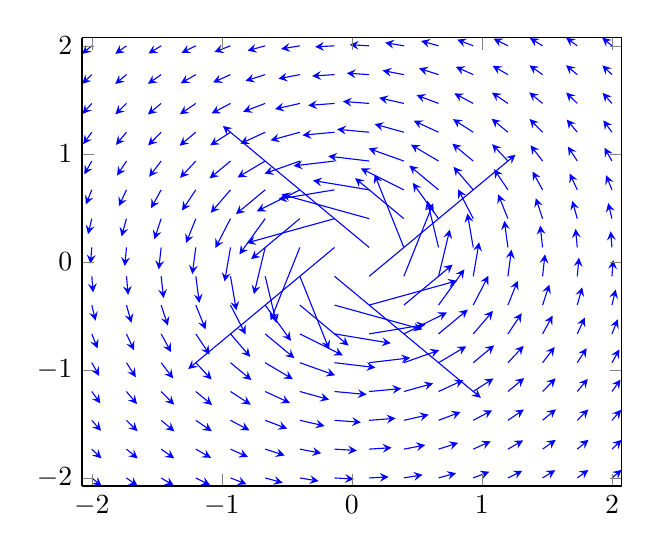
\begin{tikzpicture}
\begin{axis}[view={0}{90},domain=-2:2]
\addplot3 [blue,-stealth,samples=16,
        quiver={
            u={-1*y/(x^2 + y^2)},
            v={x/(x^2 + y^2)},
            scale arrows=0.3,
        },
    ] { 1}; % use pow(x^2 + y^2,1/2) if you choose to have a real 3D plot
\end{axis}
\end{tikzpicture}
    \end{center}
\end{example}

\begin{example}
    However, the vortex field $\bm{F} = \langle \frac{-y}{x^2 + y^2}, \frac{x}{x^2 + y^2} \rangle$ \textbf{is conservative} on $\{(x,y) \ | \ x > 0\}$.
\end{example}


\begin{definition}
    A vector field $\bm{F}$ on a domain $D$ is \textbf{path-independent} if for any two points $\bm{P}, \bm{Q} \in D$, then 
    $$\int_{C_1} \bm{F} \cdot d\bm{r} = \int_{C_2} \bm{F} \cdot d\bm{r}$$
    For any two paths $C_1, C_2$ in $D$ that start at $\bm{P}$ and end at $\bm{Q}$.
\end{definition}
    
    \begin{motivating}
        Are there any non-conservative path-independent vector fields?
    \end{motivating}
    
       
    \begin{theorem}
    A vector field $\bm{F}$ in an open, connected domain $D$ is path-independent if and only if it is conservative.
    \end{theorem}

    \begin{proof}
        
    \end{proof}


\subsection{Vector flux line integrals}

\begin{motivating}
    Imagine that $C$ is a cell membrane - how much water flows through $C$?
\end{motivating}

\begin{motivating}
    How do we compute flux line integrals?
\end{motivating}

\begin{definition}
    Given an oriented curve $C$ in $\R^2$, we say that the \textbf{positive direction \textit{across} $C$} is the direction that goes left to right from the perspective of the positive orientation \textit{along $C$}.
        
    %\pause
    
    
    Let $\bm{n}(p)$ denote the unit vector normal to $C$ at the point $p$, pointing in the positive direction across $C$.  
    
    \end{definition}

\begin{definition}
    Let $\bm{F}$ be a vector field.  The \textbf{normal component} of $\bm{F}$ at $p \in C$ is the dot product 
    $$\bm{n}(p) \cdot \bm{F}(p)$$
    
    \end{definition}

\begin{theorem}
    The \textbf{flux integral} of a vector field $\bm{F}$ along an oriented curve $C$ in $\R^2$ is the integral of the normal component of $\bm{F}$:
    $$\int_C \bm{F} \cdot \bm{n} \ ds$$
    
    \end{theorem}

\begin{remark}
    Let $\bm{r}(t) = \langle x(t), y(t)\rangle$ be a positive oriented regular parametrization of an oriented curve $C$. Observe that $\bm{N}(t) = \langle y'(t), -x'(t) \rangle$ is normal to $C$.  Therefore,
    $$\bm{n}(t) = \frac{\bm{N}(t)}{||\bm{N}(t)||}$$
    \end{remark}

\begin{theorem}
    Let $\bm{r}(t) = \langle x(t), y(t)\rangle$ be a positive oriented regular parametrization of an oriented curve $C$ for $a \leq t \leq b$.  Then
    $$\int_C \bm{F} \cdot \bm{n} \ ds = \int_a^b \bm{F}(\bm{r}(t)) \cdot \bm{N}(t) \ dt$$
    
    \end{theorem}

\begin{example}
    Calculate the flux of the velocity vector field $\bm{v} = \langle 3+2y -\frac{y^2}{3}, 0 \rangle$ (in cm/sec) across the quarter ellipse $\bm{r}(t) = \langle 3\cos(t), 6\sin(t) \rangle$ for $0 \leq t \leq \frac{\pi}{2}$.
\end{example}



\subsection{Exercises}

\begin{problem}
    Let $\bm{F}(x,y) = \langle \frac{1}{x}, \frac{-1}{y} \rangle$.  Calculate the work against $F$ required to move an object in from $(1,1)$ to $(2,4)$ along the parabola $y=x^2$, and from $(2,4)$ to $(3,4)$ along a straight line path.
\end{problem}

\begin{problem}
    Consider the unit cube of vertices at the points $(0,0,0)$ and $(1,1,1)$.  Pick any path along the edges of the cube that starts at $(0,0,0)$ and ends at $(1,1,1)$.  Let $\bm{F}(x,y,z) = \langle e^z, e^{x-y}, e^y \rangle$.  Calculate the line integral of $\bm{F}$ along your chosen path.
\end{problem}

\begin{problem}
    Consider the triangle with vertices $A = (2,0,0)$, $B = (0,4,0)$, $C = (0,0,6)$.  Let $\bm{F}(x,y,z) = \langle e^z, e^{x-y}, e^y \rangle$.  Calculate the line integral of $\bm{F}$ along the closed loop $ABCA$.
\end{problem}

\begin{problem}{conservative1}
Let $\bm{F} = \langle 2x+y, x \rangle$, and calculate $\int_C \bm{F} \cdot d\bm{r}$, where $\bm{r}$ is any path from $(1,2)$ to $(5,7)$.
\end{problem}

\begin{problem}{vortexconservative}
    Consider the vortex field $\bm{F} = \langle \frac{-y}{x^2 + y^2}, \frac{x}{x^2 + y^2} \rangle$ on the region $\{(x,y) \ | \ x > 0\}$. Show that $\bm{F}$ is conservative on this region.  (\textbf{Hint:} Consider the function $\tan^{-1}(u)$).
\end{problem}

\begin{problem}{flux1}
     Calculate the flux of the vector field $\bm{F} = \langle -y, x \rangle$ across the upper half of the unit circle centered at the origin, oriented clockwise.
\end{problem}

\begin{problem}{fluxparam2}
    Find a positively oriented parametrization of the parabola $y = x^2$ for $0 \leq x \leq 1$, oriented from left to right (from $(0,0)$ to $(1,1)$). 
\end{problem}

\begin{problem}{flux2}
    Compute the flux of the vector field $\bm{F} = \langle e^y, 2x-1 \rangle$ across the parabola $y = x^2$ for $0 \leq x \leq 1$, oriented from left to right.
\end{problem}

\begin{problem}{fluxparam3}
    Find a positively oriented parametrization of the parabola $y = x^2$ for $0 \leq x \leq 1$, oriented from right to left (from $(1,1)$ to $(0,0)$). 
\end{problem}

\begin{problem}{flux3}
    Compute the flux of the vector field $\bm{F} = \langle e^y, 2x-1 \rangle$ across the parabola $y = x^2$ for $0 \leq x \leq 1$, oriented from right to left.
\end{problem}


\section{Vector surface integrals}

\begin{motivating}
    How do we compute surface integrals of vector fields?
\end{motivating}

\begin{definition}
    Let $S$ be a surface in $\R^3$. An orientation on $S$ is a continuous choice of a unit normal vector $\bm{n}(P)$ at each point $P$ on $S$.  We say that the \textbf{positive orientation \textit{across} $S$} is in the direction of the normal vector $\bm{n}$.
    
    We say that $-\bm{n}$ is the \textbf{opposite orientation} of $S$.
    
    
    We say that a surface with a choice of orientation is an \textbf{oriented surface}.
    
    \end{definition}

\begin{definition}
    Let $\bm{F}$ be a vector field in $\R^3$, and let $P = G(u_0,v_0)$ be a point on an oriented surface $S$.  The \textbf{normal component} of $\bm{F}$ at $p$ is the dot product 
    $$\bm{F}(P) \cdot \bm{n}(P)$$
    \end{definition}

\begin{definition}
    The \textbf{vector surface integral} of $\bm{F}$ over $S$ is defined as
    $$\iint_S \bm{F} \cdot d\bm{S} := \iint_S (\bm{F} \cdot \bm{n}) \ dS$$
    This is also known as the \textbf{flux} of $\bm{F}$ across (or through) $S$.
    \end{definition}

    \begin{definition}
    For a fluid with velocity vector field $\bm{v}$, the flow rate across $S$ (in volume/time) is given by 
    $$\iint_S \bm{v} \cdot d\bm{S}$$
    \end{definition}

\begin{theorem}
    If $-S$ denotes $S$ with the opposite orientation, then $$\iint_{-S} (\bm{F} \cdot \bm{n}) \ dS = -\iint_S (\bm{F} \cdot \bm{n}) \ dS$$
    \end{theorem}

Recall that given a \textbf{regular} parametrization $G(u,v)$ of $S$, then a normal vector at a point $P = G(u_0,v_0)$ on $S$ is determined by 
    $$\bm{N}(P) =  \frac{\partial G}{\partial u}(u_0,v_0) \times \frac{\partial G}{\partial v}(u_0,v_0)$$ 

\begin{definition}
    An \textbf{oriented parametrization} of a surface $S$ is a parametrization $G(u,v)$, with the orientation of $S$ determined by the unit normal vector $$\bm{n}(P) = \frac{\bm{N}(P)}{||\bm{N}(P)||}$$
    
    
    Given an oriented parametrization, we say that the \textbf{positive orientation \textit{of} $S$} is in the direction of the normal vector $\bm{N}$.
    
    \vspace{1em}
    
    $-\bm{N}$ gives the opposite (or negative) orientation of $S$.
    
    \end{definition}

\begin{remark}
    
    \textbf{Warning:} Not every surface is orientable, and not every parametrization is an oriented parametrization!    
    \end{remark}

\begin{center}
%    \begin{tikzpicture}[scale=0.6]
%    \begin{axis}[hide axis,
%    colormap/cool,view={60}{30}, width=15cm, axis equal image]
%        % Draw sphere (example from the pgfplots manual)
%        \addplot3[
%            surf, z buffer=sort, colormap/cool, point meta=-z,
%            samples=20, domain=-1:1, y domain=0:2*pi
%        ]
%        (
%            {(1+ x*cos(deg(y)/2))*cos(deg(y))}, % X coordinate
%            {(1+ x*cos(deg(y)/2))*sin(deg(y))}, % Y coordinate
%            sin(deg(y)/2)                           % Z (vertical) coordinate
%        );
%    \end{axis}
%\end{tikzpicture}
        
    \end{center}

 \begin{theorem}
    Let $G(u,v) : D \to \R^3$ be an oriented parametrization of a surface $S$.  Assume that $G$ is one-to-one and regular, except possibly at points on the boundary of $D$.  Then
    $$\iint_S (\bm{F} \cdot \bm{n}) \ dS = \iint_D \bm{F}(G(u,v)) \cdot \bm{N}(u,v) \ du \ dv$$
    
    \end{theorem}

\begin{example}
    Calculate $\iint_S \bm{F} \cdot d\bm{S}$, where $\bm{F} = \langle 0, 0, x\rangle$, and $S$ is the surface with parametrization $G(u,v) : D \to \R^3$, 
    $$G(u,v) = (u^2,v,u^3-v^2)$$
    for $D = \{(u,v) \ |\  0 \leq u \leq 1, \ 0 \leq v \leq 1\}$, and $S$ is oriented with upward-pointing normal vectors.
\end{example}

\subsection{Exercises}

\begin{problem}{surfaceflux1}
     Find a \textbf{positively oriented} parametrization of the upper hemisphere of the unit sphere, centered at the origin, with outward pointing normal vectors.
\end{problem}

\begin{problem}{surfaceflux2}
     Calculate the flux of $\bm{F} = \langle z, x, 1 \rangle$ across the upper hemisphere of the unit sphere, centered at the origin, with outward pointing normal vectors.
\end{problem}




\section{Green's theorem, Stokes' theorem, and the divergence theorem}

\begin{motivating}
    How can we generalize the fundamental theorem of single variable calculus?
\end{motivating}

\begin{theorem}[Fundamental Theorem for Conservative Vector Fields]
    Let $\bm{F} = \nabla f$ be a conservative vector field on a domain $D$. If $\bm{r}$ is a path along a \textbf{closed curve} $C$ in $D$, then the circulation is zero:
    $$\oint_C \bm{F} \cdot d\bm{r} = 0$$
    \end{theorem}

What if $\bm{F}$ is \textbf{not} conservative?  Can we still calculate $\oint_C \bm{F} \cdot d\bm{r}$?


\subsection{Green's theorem}


\begin{definition}
    A \textbf{simple} closed curve $C$ is a closed curve that does not intersect itself.
\end{definition}

\begin{theorem}[Green's theorem]
    Let $D$ be a region in $\R^2$ such that $\partial D$ is a disjoint union of simple closed curves, with $\partial D$ oriented so that $D$ is always to the left.
    
    \vspace{1em}
    
    
    Suppose $\bm{F} = \langle F_1, F_2 \rangle$ is a smooth vector field on $D$.  Then
    $$\oint_{\partial D} \bm{F} \cdot d\bm{r} = \iint_D \left(\frac{\partial F_2}{\partial x} - \frac{\partial F_1}{\partial y}\right) \ dA$$
    
    \end{theorem}


\begin{remark}
    Green's theorem is a generalization of the fundamental theorem for conservative vector fields.
\end{remark}

\begin{theorem}[Additivity of circulation]
    Let $D$ be a region in $\R^2$ such that $\partial D$ is a simple closed curve, oriented counterclockwise.  If we decomposes a domain $D$ into two domains $D_1$ and $D_2$ who intersect only on their boundaries, $\partial D_1$ and $\partial D_2$, then
    $$\oint_{\partial D} \bm{F} \cdot d\bm{r} = \oint_{\partial D_1} \bm{F} \cdot d\bm{r} + \oint_{\partial D_2} \bm{F} \cdot d\bm{r}$$
    
    \end{theorem}

%    \begin{figure}
%        \centering
%        \includegraphics[scale=0.4]{pictures/greenstheoremboundary.png}
%    \end{figure}
    
\begin{motivating}
How does Green's theorem relate to flux integrals and the divergence of a vector field in $\R^2$?
\end{motivating}


\begin{theorem}
    Let $\bm{r}(t) = \langle x(t), y(t)\rangle$ be a positive oriented regular parametrization of an oriented curve $C$ for $a \leq t \leq b$.  Then
    $$\int_C \bm{F} \cdot \bm{n} \ ds = \int_a^b \bm{F} \cdot \left\langle \frac{y'(t)}{||\bm{r}'(t)||}, \frac{-x'(t)}{||\bm{r}'(t)||} \right\rangle \ ||\bm{r}'(t)||\ dt$$
    Thus
    $$\oint_{\partial D} \bm{F} \cdot \bm{n} \ ds = \oint_{\partial D} F_1 \ dy - F_2 \ dx$$
    \end{theorem}

\begin{theorem}[Green's theorem, flux form]
    Let $D$ be a region in $\R^2$ such that $\partial D$ is a simple closed curve, oriented counterclockwise.  Suppose $\bm{F} = \langle F_1, F_2 \rangle$ is a smooth vector field on $D$.
    Then
    $$\oint_{\partial D} \bm{F} \cdot \bm{n} \ ds = \iint_D \textnormal{div}(\bm{F}) \ dA$$
        \end{theorem}

\begin{corollary}
    Suppose $\bm{F} = \langle F_1, F_2 \rangle$ is a smooth vector field, and let $P$ be a point in $\R^2$.  Let $D = B_\varepsilon(P)$ be a small disk around $P$. 
    
    Then
    $$\oint_{\partial D} \bm{F} \cdot \bm{n} \ ds = \iint_D \textnormal{div}(\bm{F}) \ dA \approx \textnormal{div}(\bm{F})(P) \cdot \textnormal{area}(D)$$

    Thus, $$\textnormal{div}(\bm{F})(P) \approx \frac{1}{\textnormal{area}(D)}\oint_{\partial D} \bm{F} \cdot \bm{n} \ ds$$
    Therefore, the divergence of a 2D vector field $\bm{F}$ measures the \textbf{outward flux} of $\bm{F}$.
    \end{corollary}

\begin{theorem}[Green's theorem, circulation form]
    Let $D$ be a region in $\R^2$ such that $\partial D$ is a simple closed curve, oriented counterclockwise.  Suppose $\bm{F} = \langle F_1, F_2 \rangle$ is a smooth vector field on $D$.
    Then
    $$\oint_{\partial D} \bm{F} \cdot d\bm{r} = \iint_D \textnormal{curl}_z(\bm{F}) \ dA$$
        \end{theorem}

\begin{corollary}
    Suppose $\bm{F} = \langle F_1, F_2 \rangle$ is a smooth vector field, and let $P$ be a point in $\R^2$.  Let $D = B_\varepsilon(P)$ be a small disk around $P$. 
    
    Then
    $$\oint_{\partial D} \bm{F} \cdot d\bm{r} = \iint_D \textnormal{curl}_z(\bm{F}) \ dA \approx \textnormal{curl}_z(\bm{F})(P) \cdot \textnormal{area}(D)$$

    Thus, $$\textnormal{curl}_z(\bm{F})(P) \approx \frac{1}{\textnormal{area}(D)}\oint_{\partial D} \bm{F} \cdot d\bm{r}$$
    Therefore, the curl of a 2D vector field $\bm{F}$ measures the \textbf{circulation} of $\bm{F}$.
    \end{corollary}

\subsection{Stokes' theorem}

\begin{motivating}
    Is there an analogue or generalization of Green's theorem in 3 dimensions?
\end{motivating}

\begin{remark}
    A \textbf{simple} closed curve $C$ in $\R^3$ can be thought of as the boundary of a surface $S$ in $\R^3$.
    \end{remark}

\begin{definition}
    A subset $M \subset \R^n$ is a \textbf{differentiable $k$-dimensional manifold \textit{with boundary}} embedded in $\R^n$  if for all $\bm{z} \in M$, \underline{either}
    
    \begin{enumerate}
        \item  there exists an open neighborhood $U \subset \R^n$ such that there exists a $C^1$-mapping $F : U \to \R^{n-k}$ such that
                \begin{itemize}
            \item $M \cap U = \{\bm{z} \in U \ | \ F(\bm{z}) = \bm{0} \}$
            \item $[DF(\bm{z})]$ is surjective
        \end{itemize}

        \item \underline{OR} there exists an open neighborhood $V \subset \R^n$ such that there exists a $C^1$-mapping $G : V \to \R^{m}$ such that
        \begin{itemize}
            \item $G(\bm{z}) = \bm{0}$
            \item $M \cap V = \{\bm{x} \in V \ | \ G(\bm{x}) \geq \bm{0} \}$
            \item $[DG(\bm{z})]$ is surjective
        \end{itemize}
    \end{enumerate}

    We say that the set of points $\bm{z} \in M$ satisfying the latter condition are the boundary of $M$.  
    \end{definition}

\begin{example}
    The \textbf{upper half-space} $H^k \subset \R^k$ is the (closed) set $$H^k := \{ \bm{x} = \langle x_1, \cdots, x_k \rangle \ | \ x_k \geq 0\}$$
    This is a $k$-dimensional manifold with boundary $$\partial H^k =\{ \langle x_1, \cdots, x_k \rangle \ | \ x_k = 0\} $$
    \end{example}

\begin{example}
     What is the boundary of the hemisphere? $$S_+ = \{(x,y,z) \ | \ x^2 + y^2 + z^2 = 1, z \geq 0\}$$
\end{example}

\begin{example}
    
    What is the boundary of the solid cube in $\R^3$?
\end{example}

\begin{definition}
        If $\bm{z} \in \partial M$ satisfies the latter condition, we say that $\bm{z}$ is a \textbf{corner point of codimension $m$}.
        
        \vspace{1em}
        
        In the special case $m = 1$, then we say that $\bm{z}$ is in the \textbf{smooth boundary} of $M$ (denoted $\partial^s M$).
        
        \vspace{1em}
        
        The set of corner points that is not in $\partial^s M$ is called the \textbf{non-smooth boundary} of $M$.
    \end{definition}

\begin{proposition}
    The smooth boundary $\partial^s M$ is a $k-1$-dimensional manifold.
    \end{proposition}


    \begin{proposition}
    The non-smooth boundary of $M$ has $(k-1)$-dimensional volume 0.
    \end{proposition}

Recall that an orientation of a surface $S$ in $\R^3$ is a (continuous) choice of a unit normal vector $\bm{n}(P)$ at each point $P$ on $S$.  If $S$ is an oriented surface, then we can specify an orientation of the boundary $\partial S$.

\begin{definition}
    
    The \textbf{boundary orientation} of $\partial S$ is chosen so that if your feet are $S$, and your head is where the head of $\bm{n}(P)$ is, then the orientation of $\partial S$ is chosen so that $S$ is always to your left.
    
\end{definition}

\begin{theorem}[Stoke's Theorem]
    Let $G(u,v) : D \to \R^3$ be a positively oriented parametrization of a surface $S$.  Assume that $G$ is one-to-one and regular, except possibly at points on the boundary of $D$.  This determines an orientation on $\partial S$.
    
    \vspace{1em}
    
    Suppose $\bm{F}$ is a smooth vector field on a solid region $W$ containing $S$. Then
    $$\oint_{\partial S} \bm{F} \cdot d\bm{r} = \iint_S \textnormal{curl}(\bm{F}) \cdot dS$$
    
    \end{theorem}

    \begin{example}
    Stoke's theorem is a generalization of Green's theorem.    
    \end{example}

\begin{definition}
        A \textbf{closed surface} is a surface that has no boundary.  That is, $\partial S = \varnothing$.
    \end{definition}

\begin{corollary}
    Let $S$ be a \textbf{closed surface}.  Then $$\iint_S \textnormal{curl}(\bm{F}) \cdot dS = 0$$
    \end{corollary}

\begin{corollary}
    Suppose $\bm{F}$ is a vector field in $\R^3$, and consider a plane through $X \in \R^3$ with unit normal vector $\bm{n}$.  Let $C$ be a small circle of radius $\varepsilon$ in the plane, centered at $P$, which encloses a disk $D$ in the plane. Then
    $$\oint_{\partial D} \bm{F} \cdot d\bm{r} = \iint_D \textnormal{curl}(\bm{F}) \cdot \bm{n} \ dS \approx (\textnormal{curl}(\bm{F})(P) \cdot \bm{n}) \textnormal{area}(D)$$

    Thus, $$(\textnormal{curl}(\bm{F})(P) \cdot \bm{n}) \approx \frac{1}{\textnormal{area}(D)}\oint_{\partial D} \bm{F} \cdot d\bm{r}$$
    Therefore, the \textbf{circulation} of $\bm{F}$ in a given plane $X$ depends on the angle between $\textnormal{curl}(\bm{F})$ and $\bm{n}$.
    \end{corollary}


\begin{definition}Let $\bm{F}$ be a vector field defined on a region $W \subset \R^3$. Suppose $\bm{F} = \textnormal{curl}(\bm{A})$ for some vector field $\bm{A}$.  Then $\bm{A}$ is called a \textbf{vector potential} for $\bm{F}$ on $W$.
    \end{definition}
    
    %\pause
    
    \begin{remark}
    \textbf{Warning:} Vector potential functions are not unique.  
    \end{remark}


\begin{remark}
    If $\bm{A}$ is a vector potential for $\bm{F}$ on $W$, then under the conditions of Stoke's theorem,
    $$\iint_S \bm{F} \cdot dS = \iint_S \textnormal{curl}(\bm{A}) \cdot dS = \oint_{\partial S} \bm{A} \cdot d\bm{r}$$
    %\pause
    In other words, the surface integral of $\bm{F} = \textnormal{curl}(\bm{A})$ is \textbf{surface-independent}.
    \end{remark}


\begin{corollary}
    If $\bm{F}$ has a vector potential $\bm{A}$ on $W$, and $S$ is a closed surface in $W$, then
    $$\iint_S \bm{F} \cdot dS = 0$$
    \end{corollary}

\begin{example}
    Let $\bm{F} = \textnormal{curl}(\bm{A})$, where $\bm{A} = \langle y+z, \sin(xy), e^{xyz} \rangle$.  Let $S$ be the closed surface below, which is made out of two surfaces $S_1$ and $S_2$ with common boundary the unit circle in the $xz$-plane.
%    
%    \begin{figure}
%        \centering
%        \includegraphics[scale=0.35]{pictures/stokessurfaceexample.png}
%    \end{figure}
    Find the outward flux of $\bm{F}$ across $S_1$ and $S_2$.
\end{example}


\subsection{Divergence theorem}

\begin{definition}
    Let $S$ be a closed surface.  Then $S$ encloses a 3-dimensional region $W$.
    
    \vspace{1em}
    We say that $S$ is the \textbf{boundary} of $W$, and write $S = \partial W$.
    \end{definition}

\begin{definition}
    A closed surface $S$ is piecewise-smooth if $S$ consists of finitely many smooth surfaces that have been glued together along their boundaries.
    \end{definition}

\begin{theorem}
    Let $S$ be a closed surface that encloses a region $W \subset \R^3$, such that $S$ is piecewise smooth, and is oriented by normal vectors pointing away from $W$.  If $\bm{F}$ is a smooth vector field defined on an open region containing $W$, then 
    $$\iint_S \bm{F} \cdot d\bm{S} = \iiint_W \text{div}(\bm{F}) \ dV$$
    \end{theorem}

\begin{motivating}
    How does the divergence theorem relate to the divergence of a vector field in $\R^3$?
\end{motivating}

\begin{corollary}
    Recall that $\iint_S \bm{F} \cdot d\bm{S}$ can be intepreted as the \underline{flow rate} across $S$.  Suppose $\bm{F}$ is a vector field in $\R^3$, and consider a small sphere $S$ around the point $P \in \R^3$ with outward-pointing normal. Then
    $$\iint_S \bm{F} \cdot d\bm{S} = \iiint_W \text{div}(\bm{F}) \ dV \approx \text{div}(\bm{F})(P) \textnormal{vol}(W)$$
    
    Thus, $$\text{div}(\bm{F})(P) \approx \frac{1}{\textnormal{vol}(W)}\iint_S \bm{F} \cdot d\bm{S}$$
    Therefore, the \textbf{divergence} of $\bm{F}$ at a point $P$ can be interpreted as the outward flux of $\bm{F}$ near $P$.
    \end{corollary}

     \begin{definition}
    The \textbf{inverse-square vector field} is denoted $\bm{F}_{IS}$, with components
    $$\bm{F}_{IS} = \langle \frac{x}{(x^2+y^2+z^2)^\frac{3}{2}},\frac{y}{(x^2+y^2+z^2)^\frac{3}{2}},\frac{z}{(x^2+y^2+z^2)^\frac{3}{2}}\rangle$$
    which is defined on $\R^3 - \{(0,0,0)\}$.
    \end{definition}
    
    \begin{center}
        \begin{tikzpicture}[scale=0.6]
  \begin{axis}[
    domain=-1:1,
    samples=10,
    xmin=-1,xmax=1,
    ymin=-1,ymax=1,
    zmin=-1,zmax=1,
    ]
    \pgfplotsinvokeforeach{-1,-.5,0,.5,1}{
      \addplot3[UCLAblue,quiver,-stealth,
      point meta={sqrt((x)^2+(y)^2+(z)^2)},
      quiver={
        u={x/pow(x^2 + y^2+z^2,3/2)},
        v={y/pow(x^2 + y^2+z^2,3/2)},
        w={z/pow(x^2 + y^2+z^2,3/2)},
        scale arrows=.2}]
      (x,y,#1);
    }
  \end{axis}
\end{tikzpicture}
    \end{center}

\begin{example}
     Calculate $\text{div}(\bm{F})(P)$ for a point $P$ in $\R^3 - \{(0,0,0)\}$.
\end{example}

\begin{example}
     Compute the flux of $\bm{F}_{IS}$ out of a sphere of radius $R$ centered at the origin.

\begin{remark}
    Observe that the divergence theorem does not apply here, since $\bm{F}_{IS}$ is not smooth on the ball of radius $R$ centered on the origin.
    \end{remark}
     
\end{example}

\begin{theorem}[Flux of the inverse-square field]
    Let $S$ be a closed surface, and let $W$ be the region that it encloses.  Let $\bm{F}_{IS}$ be the inverse-square vector field, defined on $\R^3 - \{(0,0,0)\}$.  Then
    $$\iint_S \bm{F}_{IS} \cdot d\bm{S} = \left\{
		\begin{array}{ll}
			0 & \text{ if } (0,0) \notin W \\
			4\pi & \text{ if } (0,0) \in W
		\end{array}
		\right.$$

    \end{theorem}

\begin{theorem}[Flow around the vortex field]
    Let $C$ be a simple closed curve oriented counterclockwise, and let $D$ be the region that it encloses.  Let $\bm{F} = \langle \frac{-y}{x^2 + y^2}, \frac{x}{x^2 + y^2} \rangle$ be the vortex field, defined on $\R^2 - \{(0,0)\}$.  Then
    $$\oint_C \bm{F} \cdot d\bm{r} = \left\{
		\begin{array}{ll}
			0 & \text{ if } (0,0) \notin D \\
			2\pi & \text{ if } (0,0) \in D
		\end{array}
		\right.$$

    \end{theorem}

\begin{motivating}
    If $\bm{G}$ is a vector field such that $\text{div}(\bm{G}) = \bm{0}$, does $\bm{G}$ have a vector potential?
    That is, can we write $\bm{G} = \textnormal{curl}(\bm{A})$ for some vector field $\bm{A}$?
    \end{motivating}
    
    \begin{theorem}
    Let $\bm{G}$ be a vector field on an open solid domain $W \subset \R^3$.  (intuitively, there are no "holes" in $W$). If $\text{div}(\bm{G}) = \bm{0}$, then $\bm{G}$ has some vector potential on $W$.
    \end{theorem}
    
    \begin{remark}
    Recall that the inverse-square vector field satisfies $\text{div}(\bm{G}) = 0$, but does not have a vector potential on $\R^3-\{(0,0,0)\}$.
    \end{remark}








    
\subsection{Cohomology}



\subsection{Exercises}

\begin{problem}{greensgeneralization}
    How is Green's theorem a generalization of the fundamental theorem for conservative vector fields?
\end{problem}

\begin{problem}{area}
    How can you use Green's Theorem to compute the area of a region $D$?
\end{problem}

\begin{problem}{verifygreen}
    Let $C$ be the unit circle, oriented counterclockwise.  Let $\bm{F} = \langle xy^2, x \rangle$.  Verify Green's theorem for $\bm{F}$ and the unit disk.
\end{problem}

\begin{problem}{stokesgeneralization}
How is Stoke's theorem a generalization of Green's theorem? (\textbf{Hint:} Compare this to the circulation form of Green's theorem.)
\end{problem}

\begin{problem}{stokescurl}
    Use Stoke's theorem to interpret the meaning of curl for vector fields in $\mathbb{R}^3$.
\end{problem}

\begin{problem}{verifystokes}
    Let $S$ be the upper hemisphere of radius $1$ with outward-pointing normal vectors, and let $\bm{F} = \langle -y, 2x, x+z\rangle$.  Verify Stoke's theorem for this surface with boundary.
\end{problem}

\begin{problem}{div1}
    Let $S$ be the closed piecewise smooth surface given by the cylinder of radius 2 and height 5, along with the disks of radius 2 at $z = 0$ and $z=5$, and let $\bm{F} = \langle y, yz, z^2\rangle$.  Compute the flux out of $S$, $$\iint_{S} \bm{F} \cdot d\bm{S}$$
\end{problem}

\begin{problem}{fluxsurf}
    Compute the flux of $$\bm{F} = \langle z^2 + xy^2, \cos(x+z), e^{-y} - zy^2 \rangle$$ outward through an arbitrary surface $S$.
\end{problem}

% \chapter{Definitions, Problems and Theorems}
% \section{Definitions}
% We can define a term like \emph{hamster}\define{hamster}, or say that the term hamster\SubIndex{hamster} appears again later.
% \begin{Verbatim}[frame=leftline]
% \chapter{Definitions, Problems and Theorems}
% \section{Definitions}
% We can define a term like \emph{hamster}\define{hamster}, 
% or say that the term hamster\SubIndex{hamster} appears again later.
% \end{Verbatim}
% Compile, for a book called \verb!filename.tex!, with
% \begin{Verbatim}[frame=leftline]
% 	makeindex filename
% \end{Verbatim}
% We add notation like when we use a variable called \(\omega\),
% we put it in the list of notation.%
% \Notation{omega}{\omega}{A variable called $\omega$}
% \begin{Verbatim}
% We add notation like when we use a variable called \(\omega\),
% we put it in the list of notation.%
% \Notation{omega}{\omega}{A variable called $\omega$}
% \end{Verbatim}
% If you use notation, compile with
% \begin{Verbatim}[frame=leftline]
% 	makeindex -s notation.gst -o not.gls not.glo  
% \end{Verbatim}

% \section{Theorems}
% You have the usual theorem environments, like \texttt{amsthm}.
% \begin{theorem}[Pythagoras]
% In any triangle with sides of lengths \(a,b,c\), \(a^2+b^2=c^2\) just when the angle opposite the side of length \(c\) is a right angle.
% \end{theorem}
% \begin{Verbatim}[frame=leftline]
% \begin{theorem}[Pythagoras]
% In any triangle with sides of lengths \(a,b,c\), 
% \(a^2+b^2=c^2\) just when the angle opposite the 
% side of length \(c\) is a right angle.
% \end{theorem}
% \end{Verbatim}






% \chapter{Citations}
% Our bibliography file looks like
% \VerbatimInput[frame=leftline]{willowtreebook.bib}
% We can cite works from the bibliography, like Homer~\cite{Homer:Iliad}, p. 12.
% \begin{Verbatim}[frame=leftline]
% We can cite works from the bibliography, like Homer~\cite{Homer:Iliad}, p. 12.
% \end{Verbatim}
% Compile with \verb!bibtex!.








% \section{Preambles}
% We can put some \LaTeX{} code before the hints:
% \begin{Verbatim}[frame=leftline]
% \RenewDocumentCommand\hintsPreamble{}{
% \par\noindent{}
% \textit{When you are describing, \\ 
% A shape, or sound, or tint; \\ 
% Don't state the matter plainly, \\ 
% But put it in a hint; \\
% And learn to look at all things, \\ 
% With a sort of mental squint.}
% \par\noindent{}---\ {Lewis Carroll}}
% \end{Verbatim}

% \RenewDocumentCommand\hintsPreamble{}{\par\noindent{}\textit{When you are describing, \\ A shape, or sound, or tint; \\ Don't state the matter plainly, \\ But put it in a hint; \\\ And learn to look at all things, \\ With a sort of mental squint.}\par\noindent{}---\ {Lewis Carroll}}
% or before the bibliography:
% \begin{Verbatim}[frame=leftline]
% \RenewDocumentCommand\bibliographyPreamble{}{
% \par\noindent
% \textit{If those books are in agreement with the Quran, 
% we have no need of them; 
% and if these are opposed to the Quran, 
% destroy them.}
% \par\noindent{}---\ {Omar}}
% \end{Verbatim}
% \RenewDocumentCommand\bibliographyPreamble{}{\par\noindent\textit{If those books are in agreement with the Quran, we have no need of them; and if these are opposed to the Quran, destroy them.}\par\noindent{}---\ {Omar}}
\end{document}